\appendix
%\newgeometry{left=1cm, right=1cm, bottom=1cm, top=1cm}

\chapter{Moduł kontrolera}
\begingroup
\renewcommand{\cleardoublepage}{}
\renewcommand{\clearpage}{}
\begin{figure}[h!]
    \begin{center}
        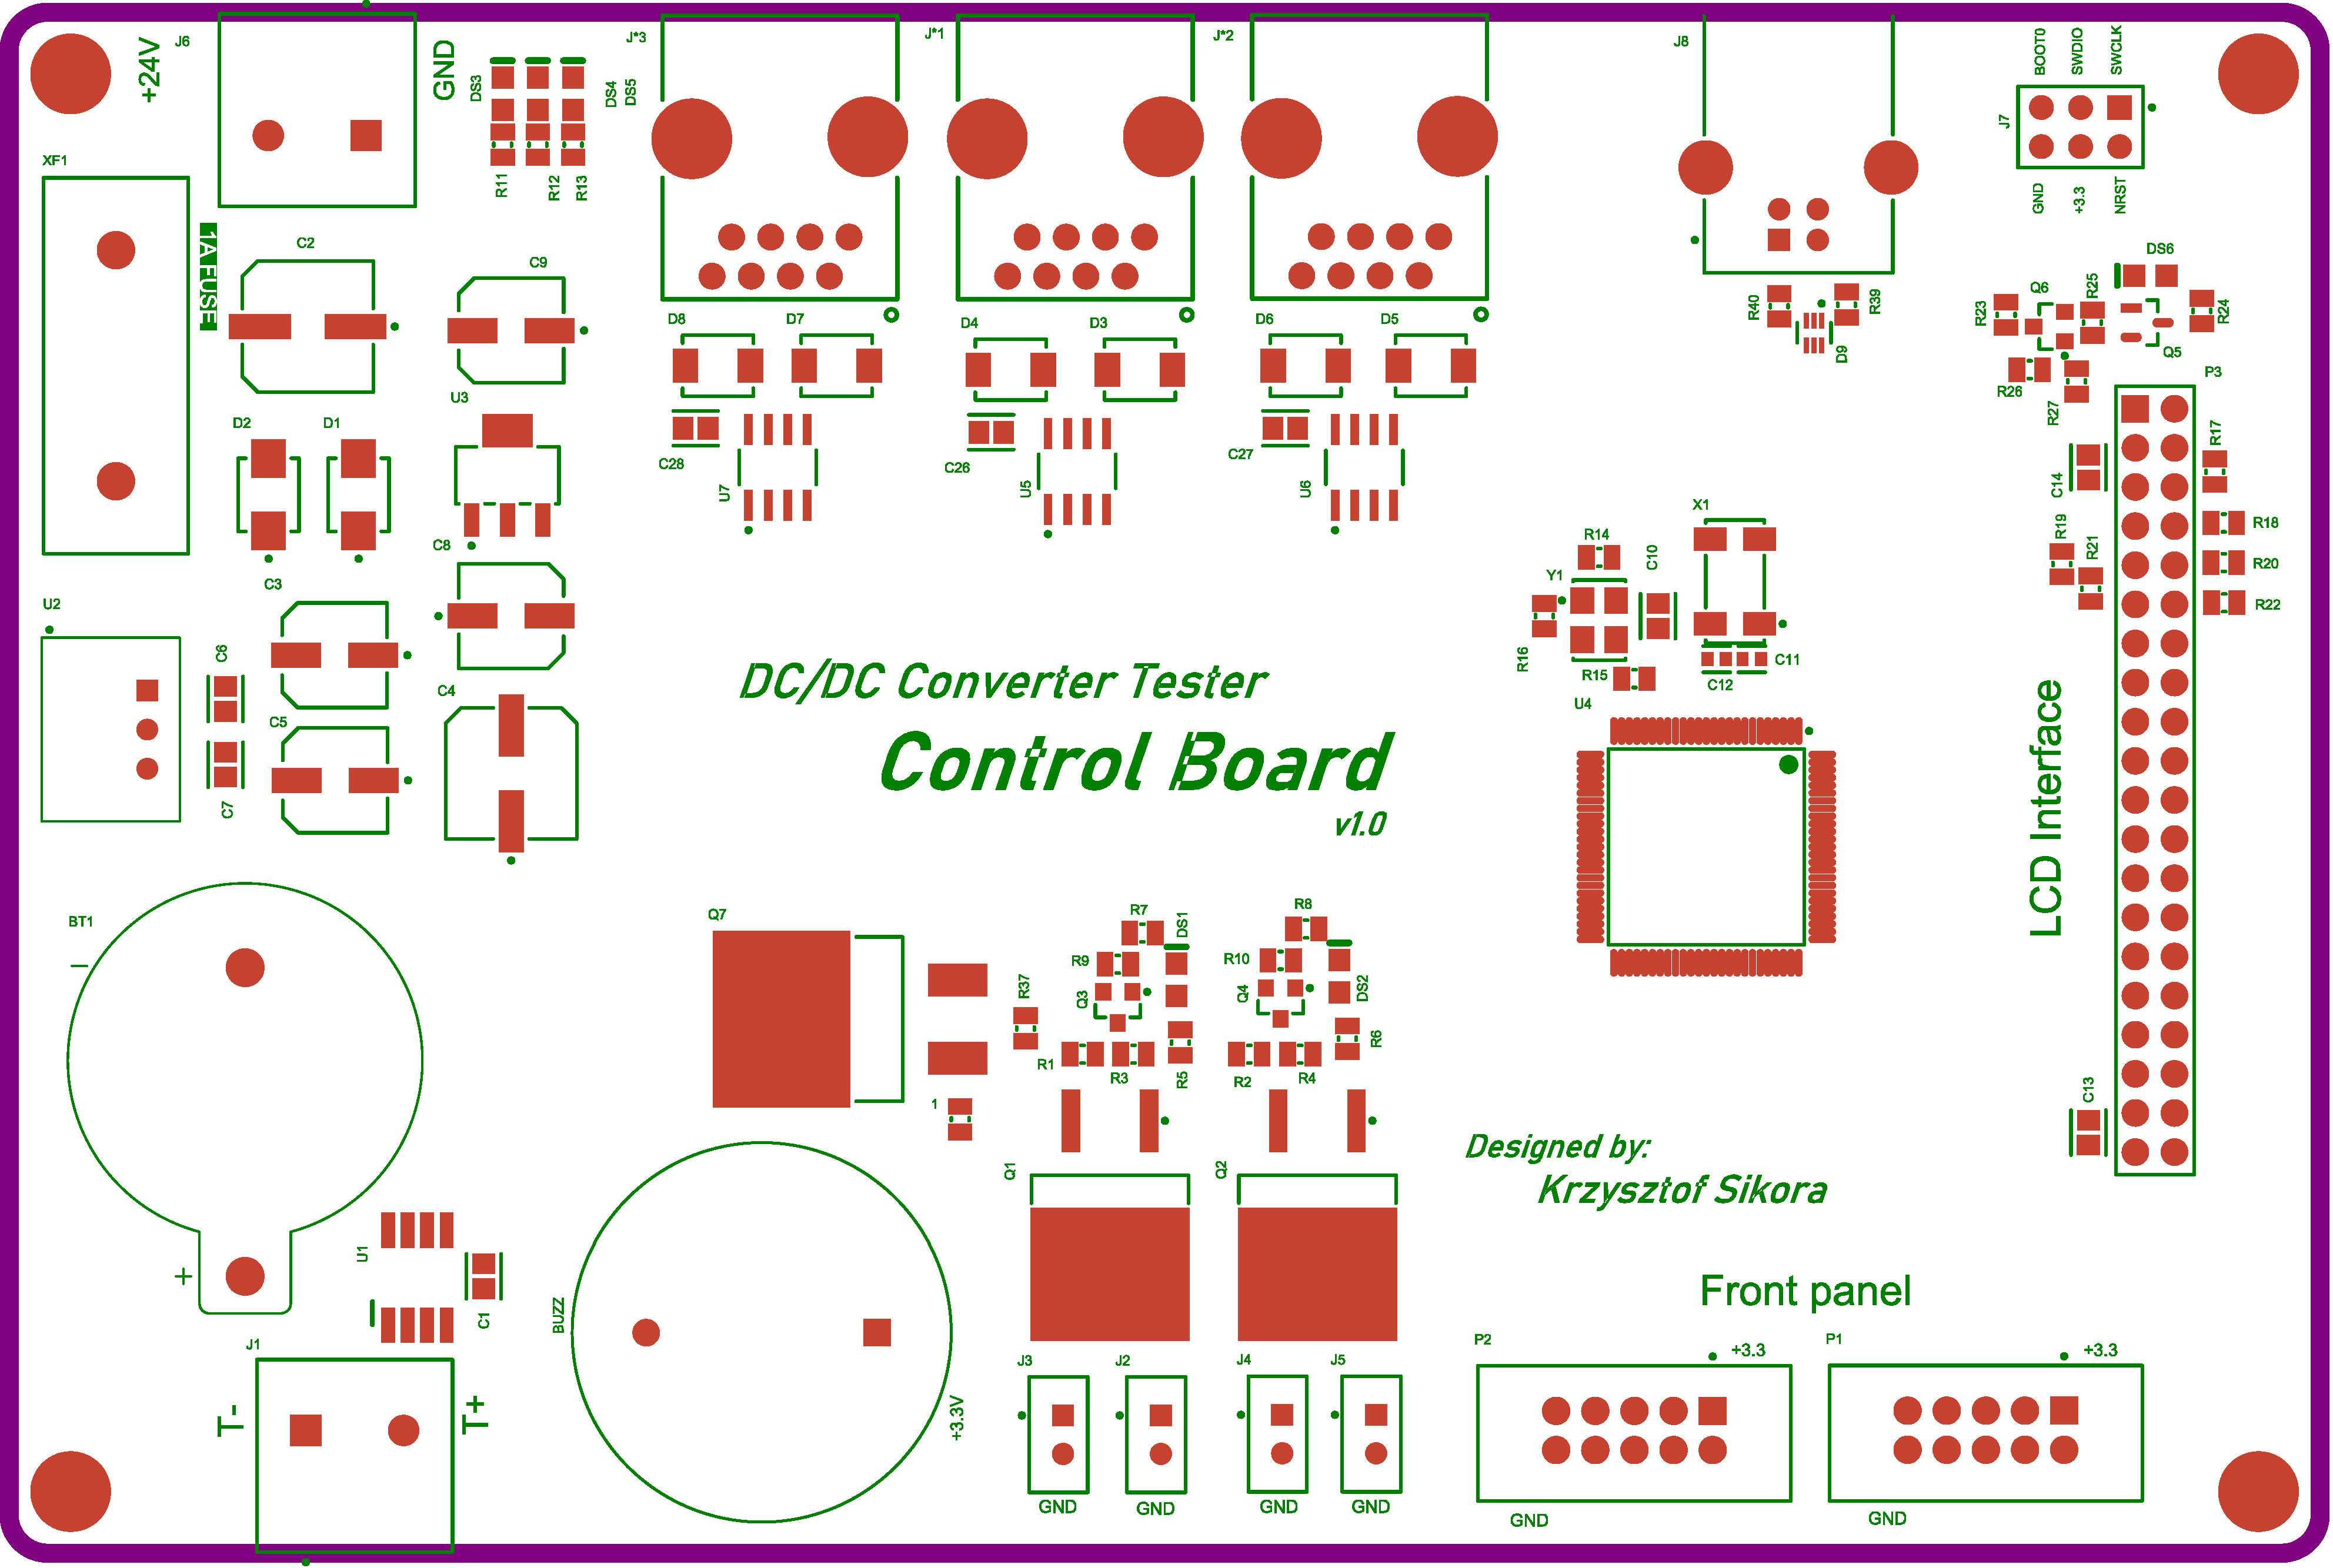
\includegraphics[width = 17cm]{zalaczniki/kontroler/Kontroler_Strona_15.jpg}
        \caption{Widok warstwy opisowej PCB.}
    \end{center}
\end{figure}

\begin{sidewaysfigure}
    \begin{center}
        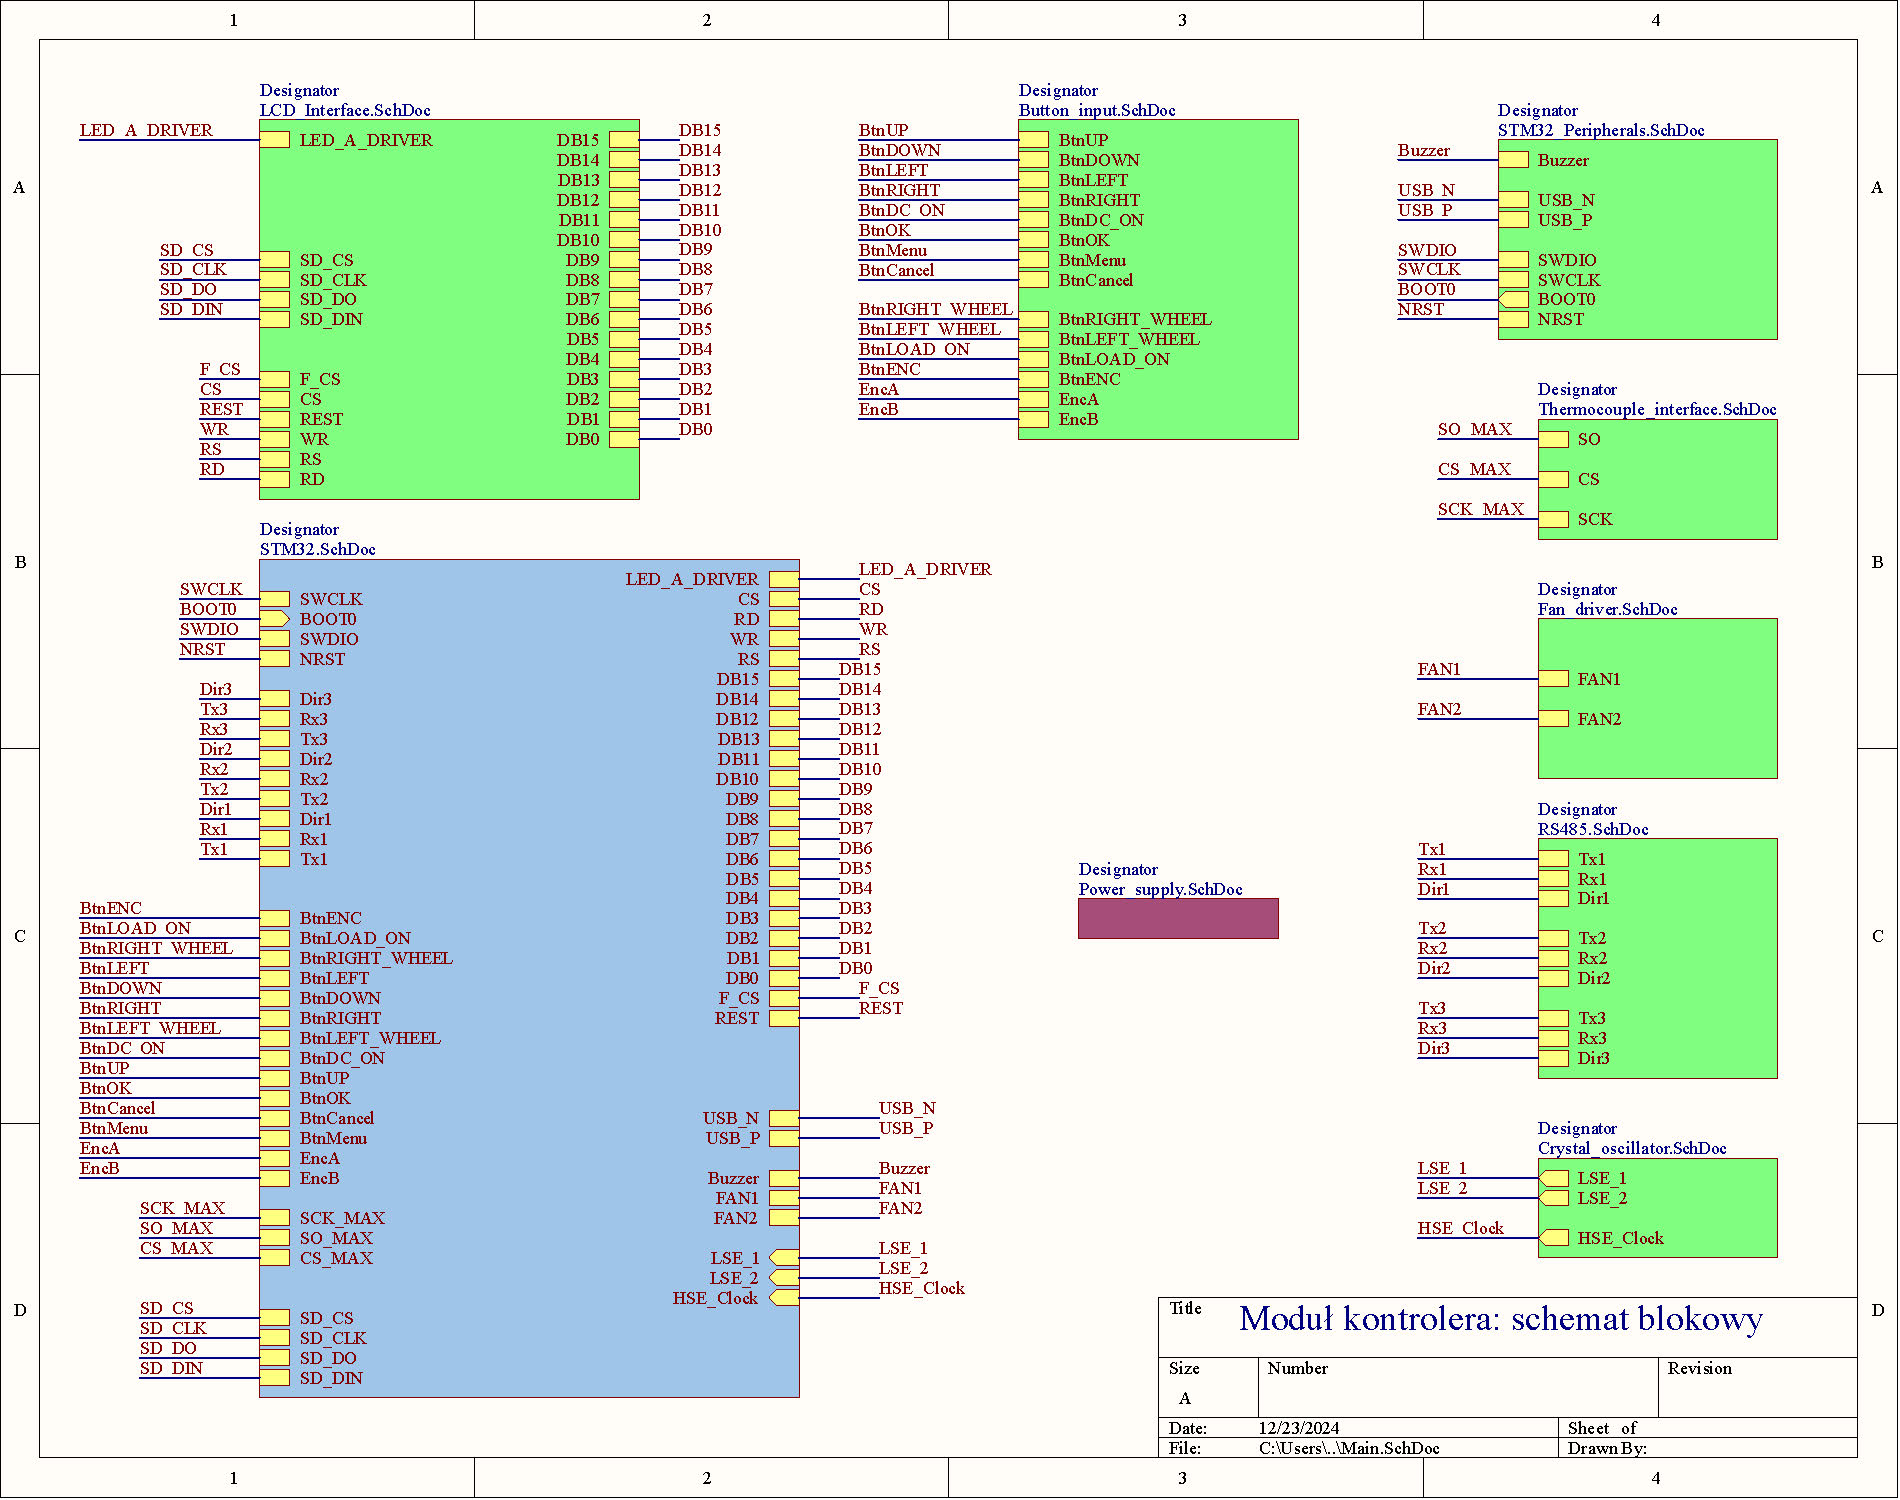
\includegraphics[width = 21cm]{zalaczniki/kontroler/Kontroler_Strona_01.jpg}
        \caption{Schemat blokowy modułu kontrolera.}
    \end{center}
\end{sidewaysfigure}

\begin{sidewaysfigure}
    \begin{center}
        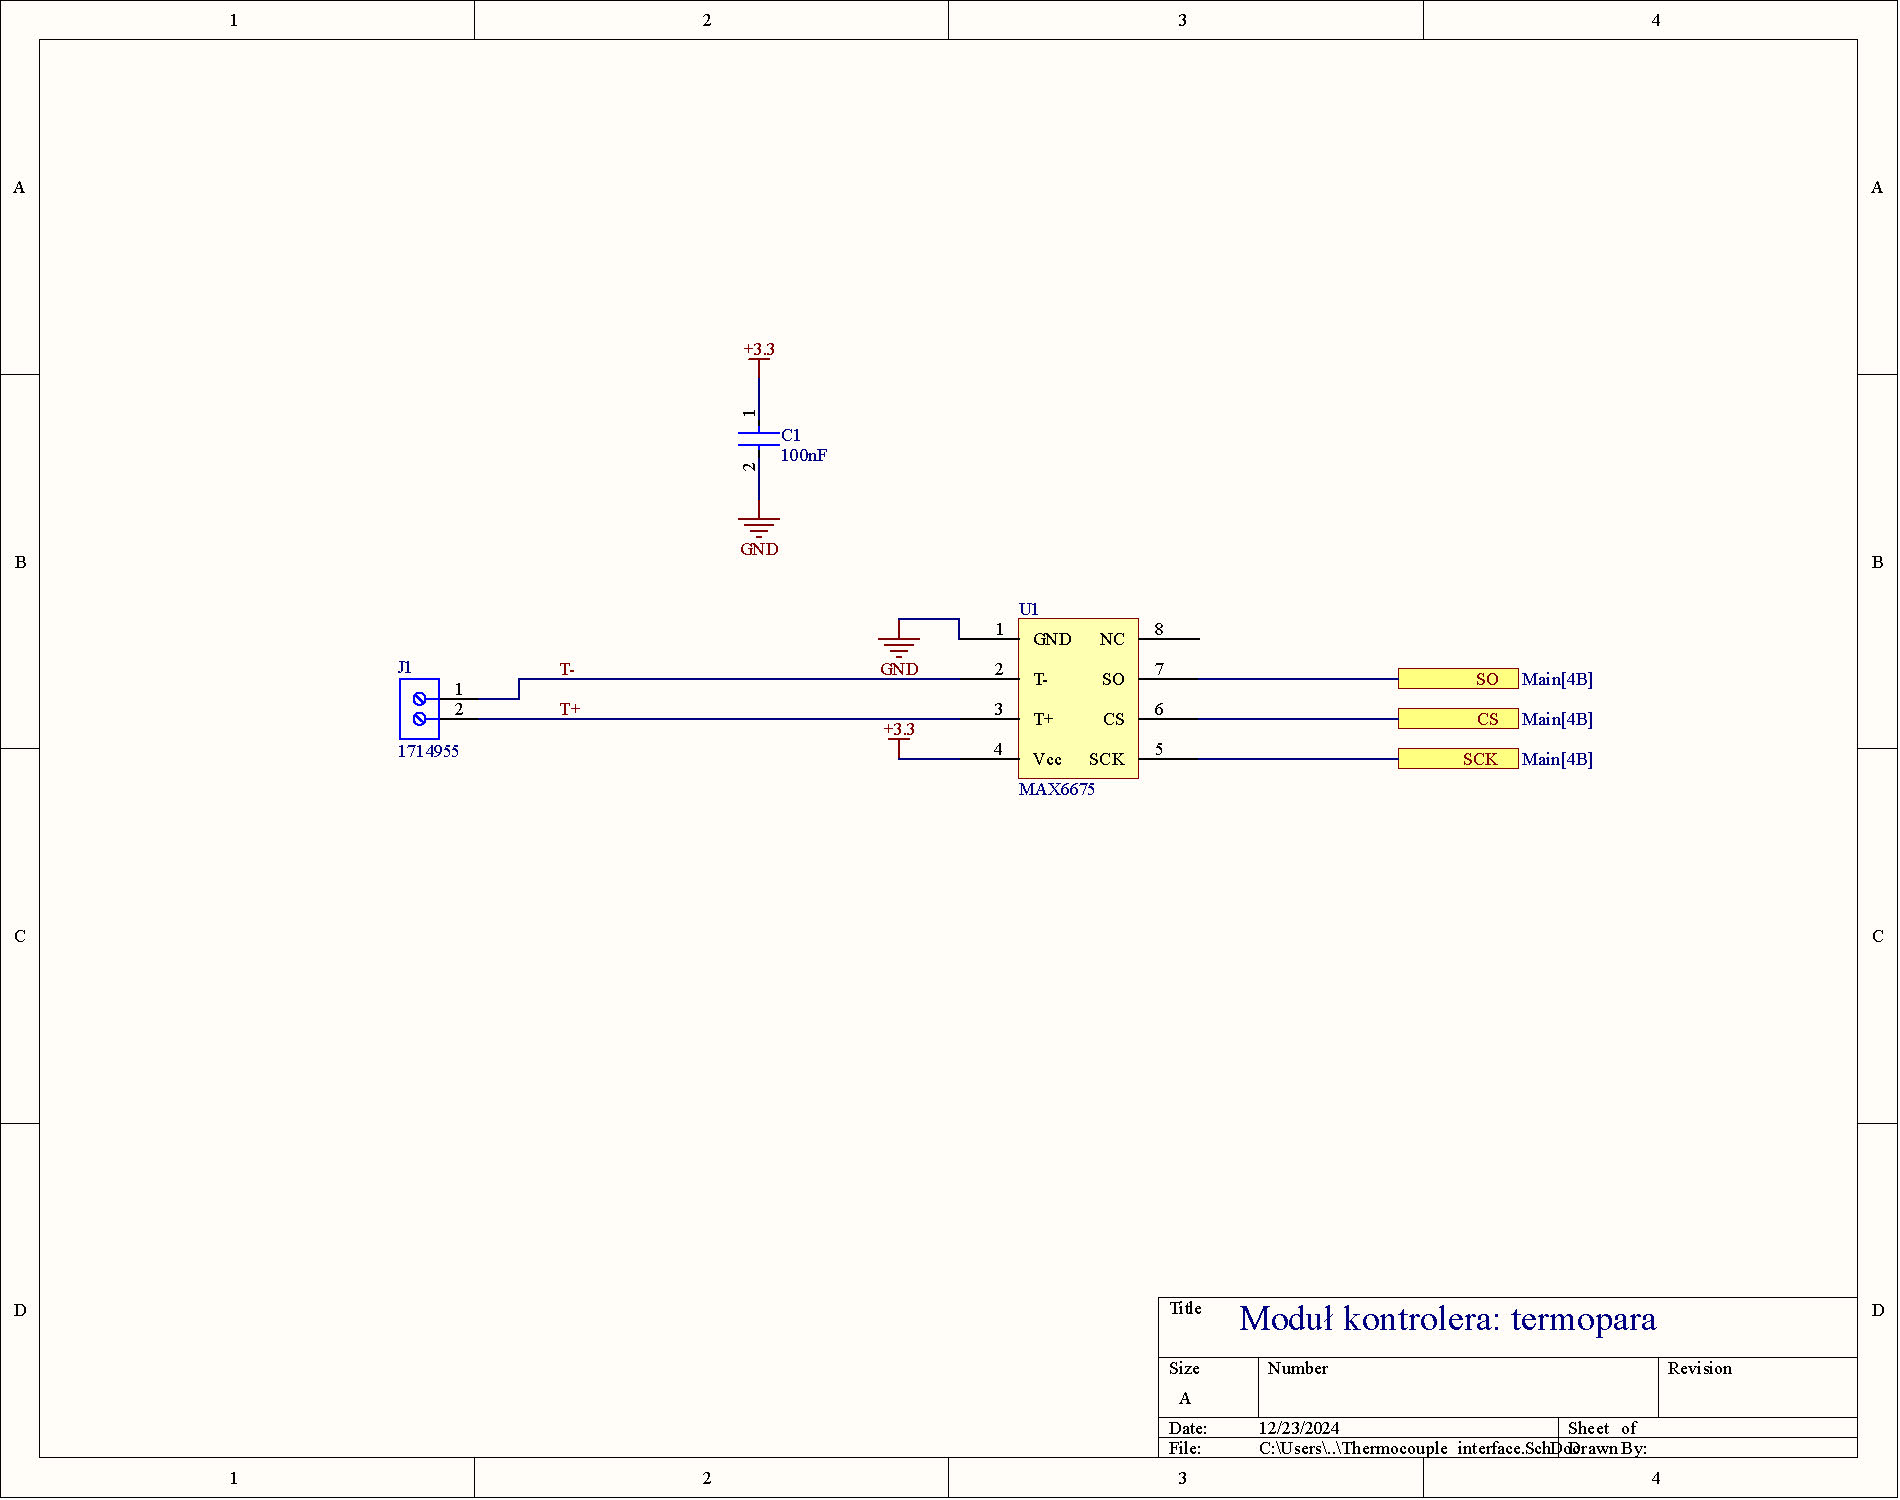
\includegraphics[width = 21cm]{zalaczniki/kontroler/Kontroler_Strona_02.jpg}
        \caption{Schemat układu termopary.}
    \end{center}
\end{sidewaysfigure}

\begin{sidewaysfigure}
    \begin{center}
        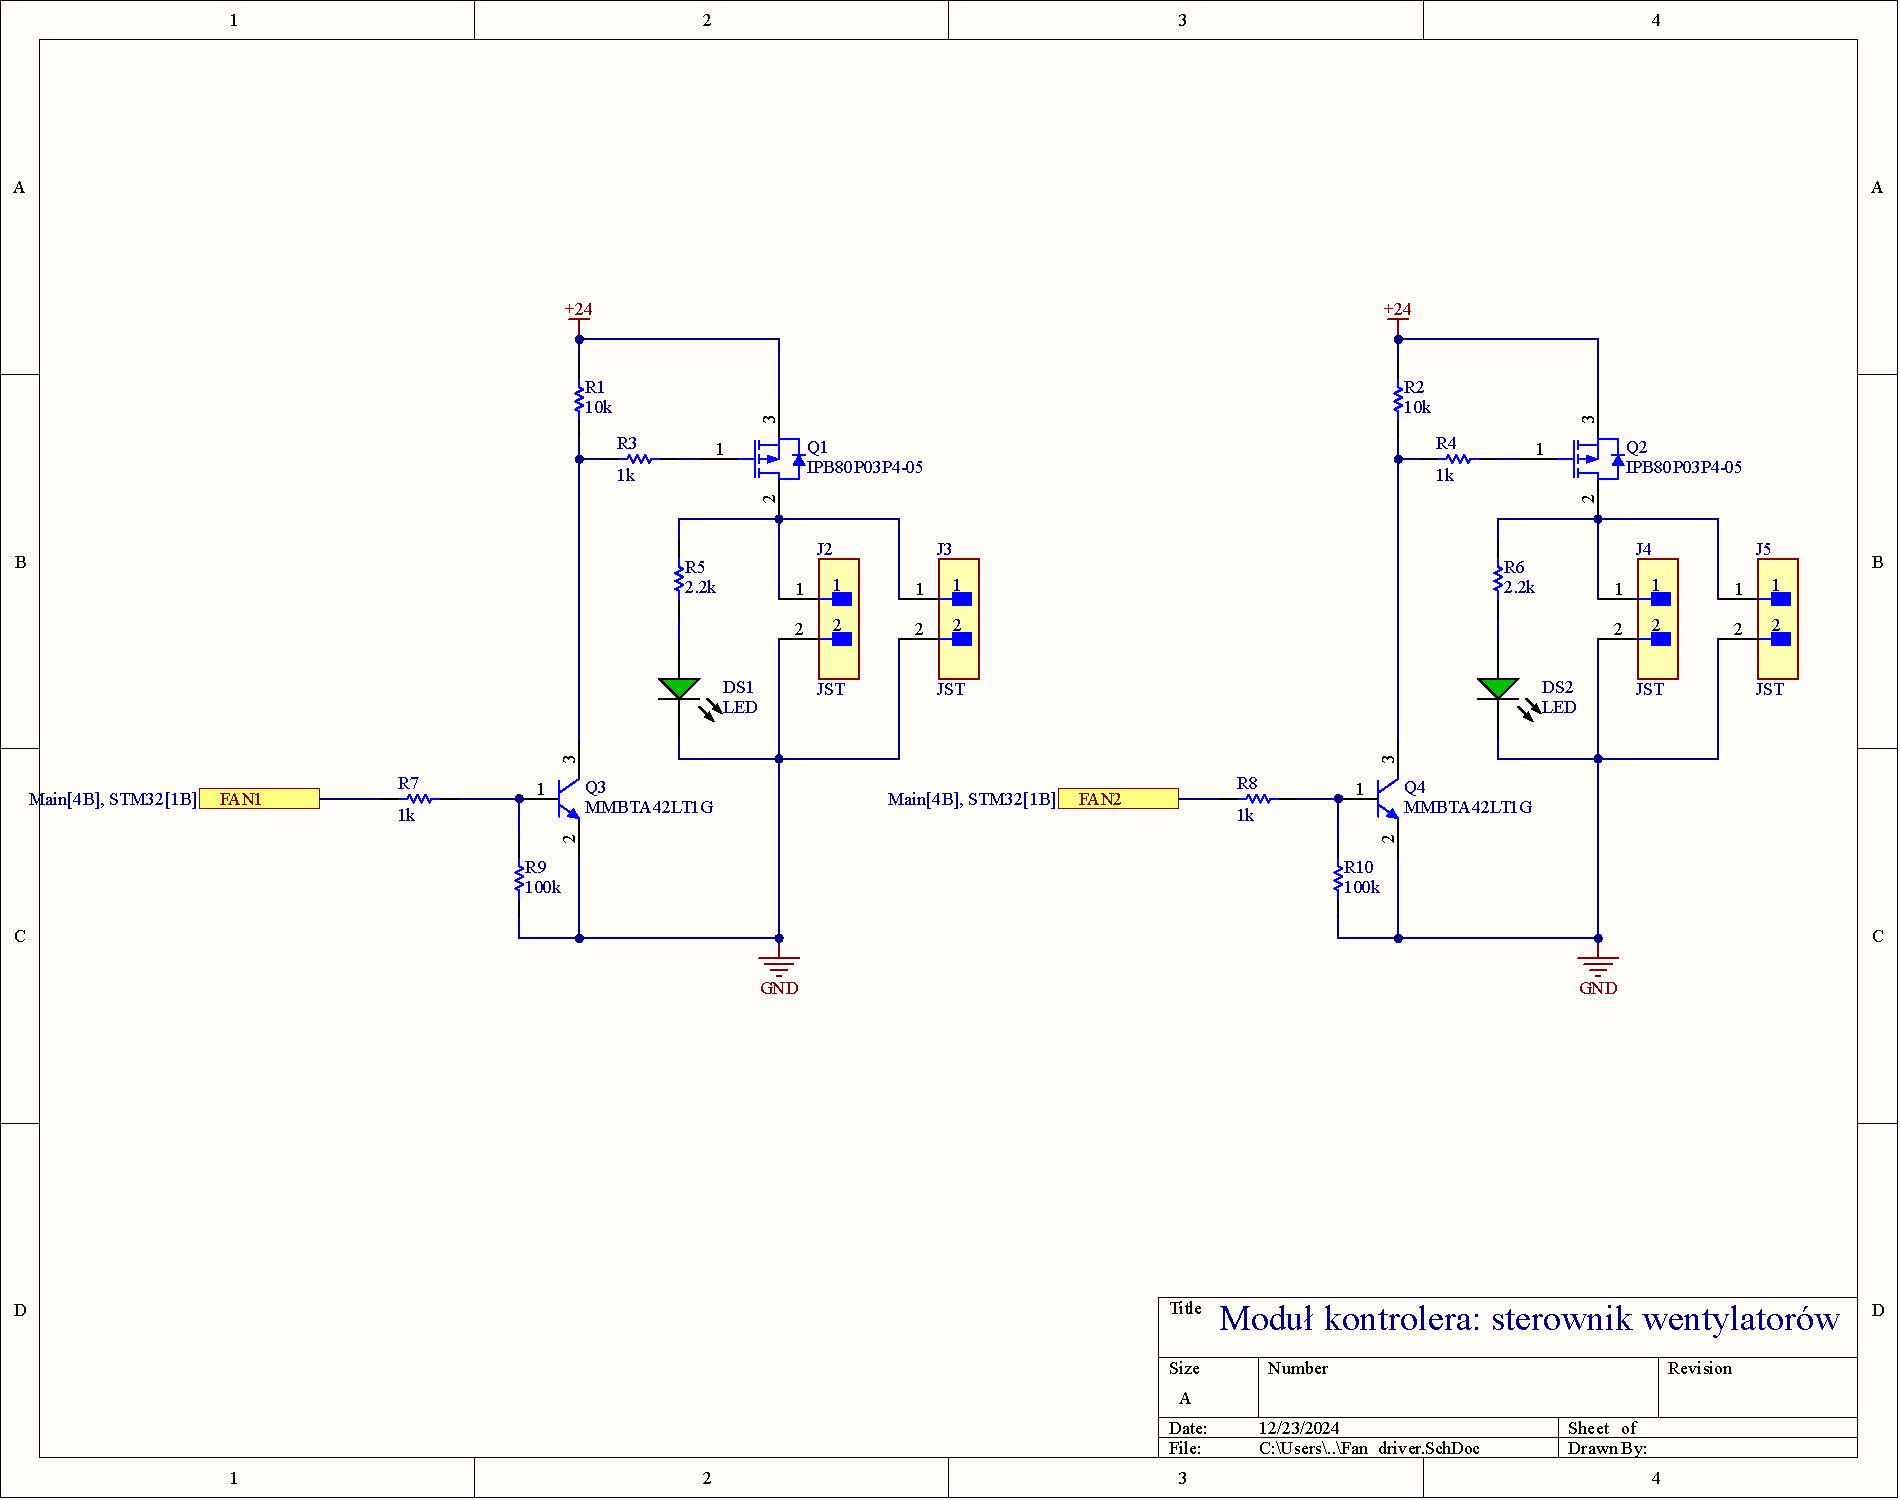
\includegraphics[width = 21cm]{zalaczniki/kontroler/Kontroler_Strona_03.jpg}
        \caption{Schemat kontrolera wentylatorów.}
    \end{center}
\end{sidewaysfigure}

\begin{sidewaysfigure}
    \begin{center}
        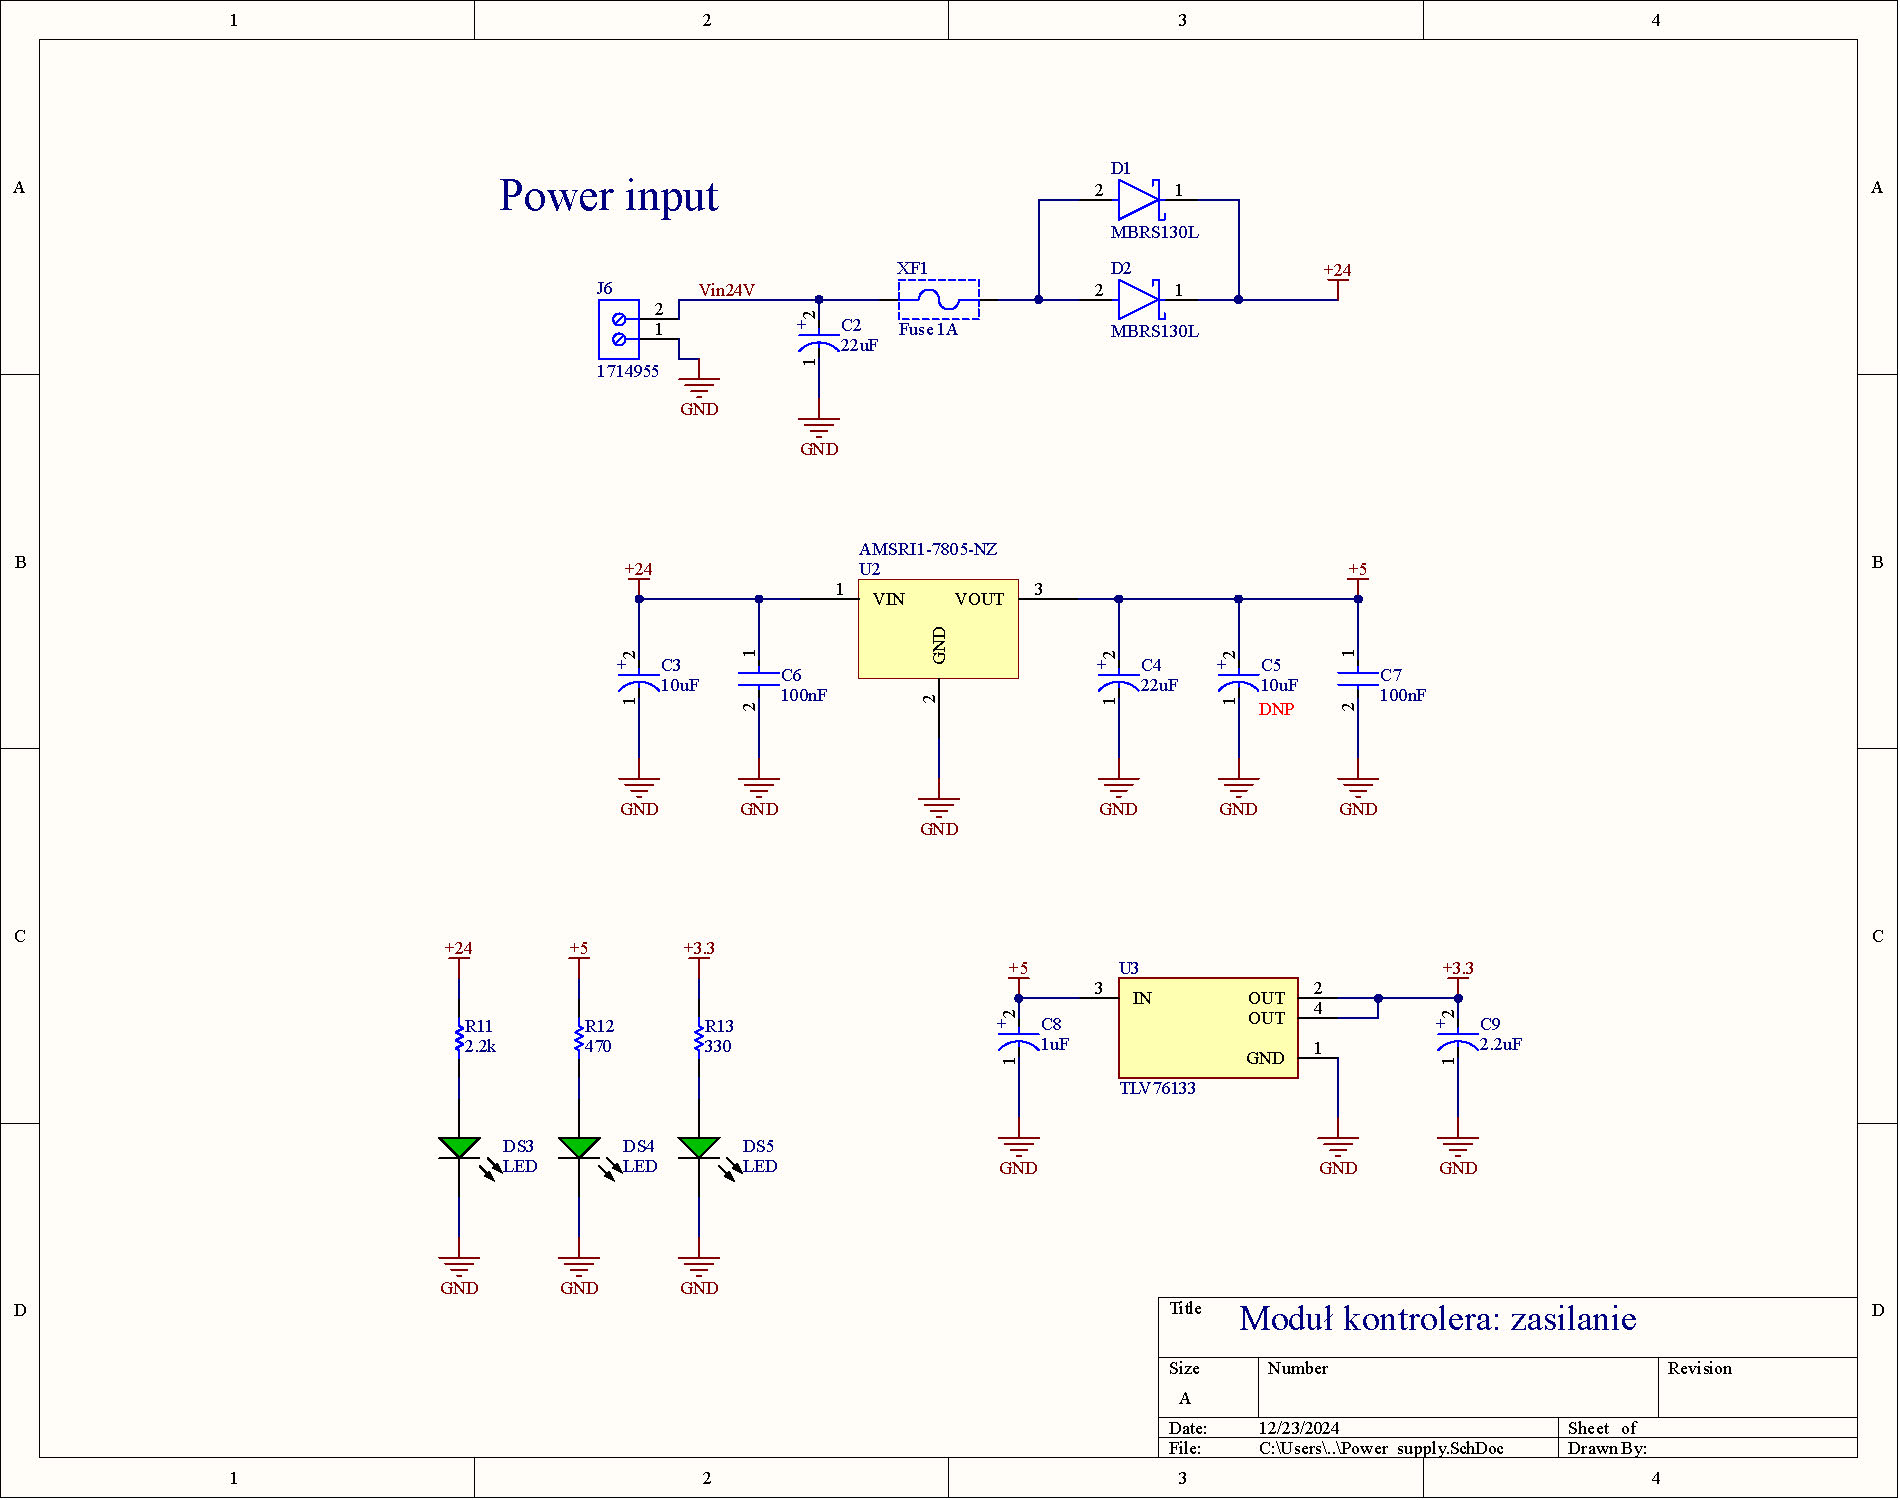
\includegraphics[width = 21cm]{zalaczniki/kontroler/Kontroler_Strona_04.jpg}
        \caption{Schemat sekcji zasilania.}
    \end{center}
\end{sidewaysfigure}

\begin{sidewaysfigure}
    \begin{center}
        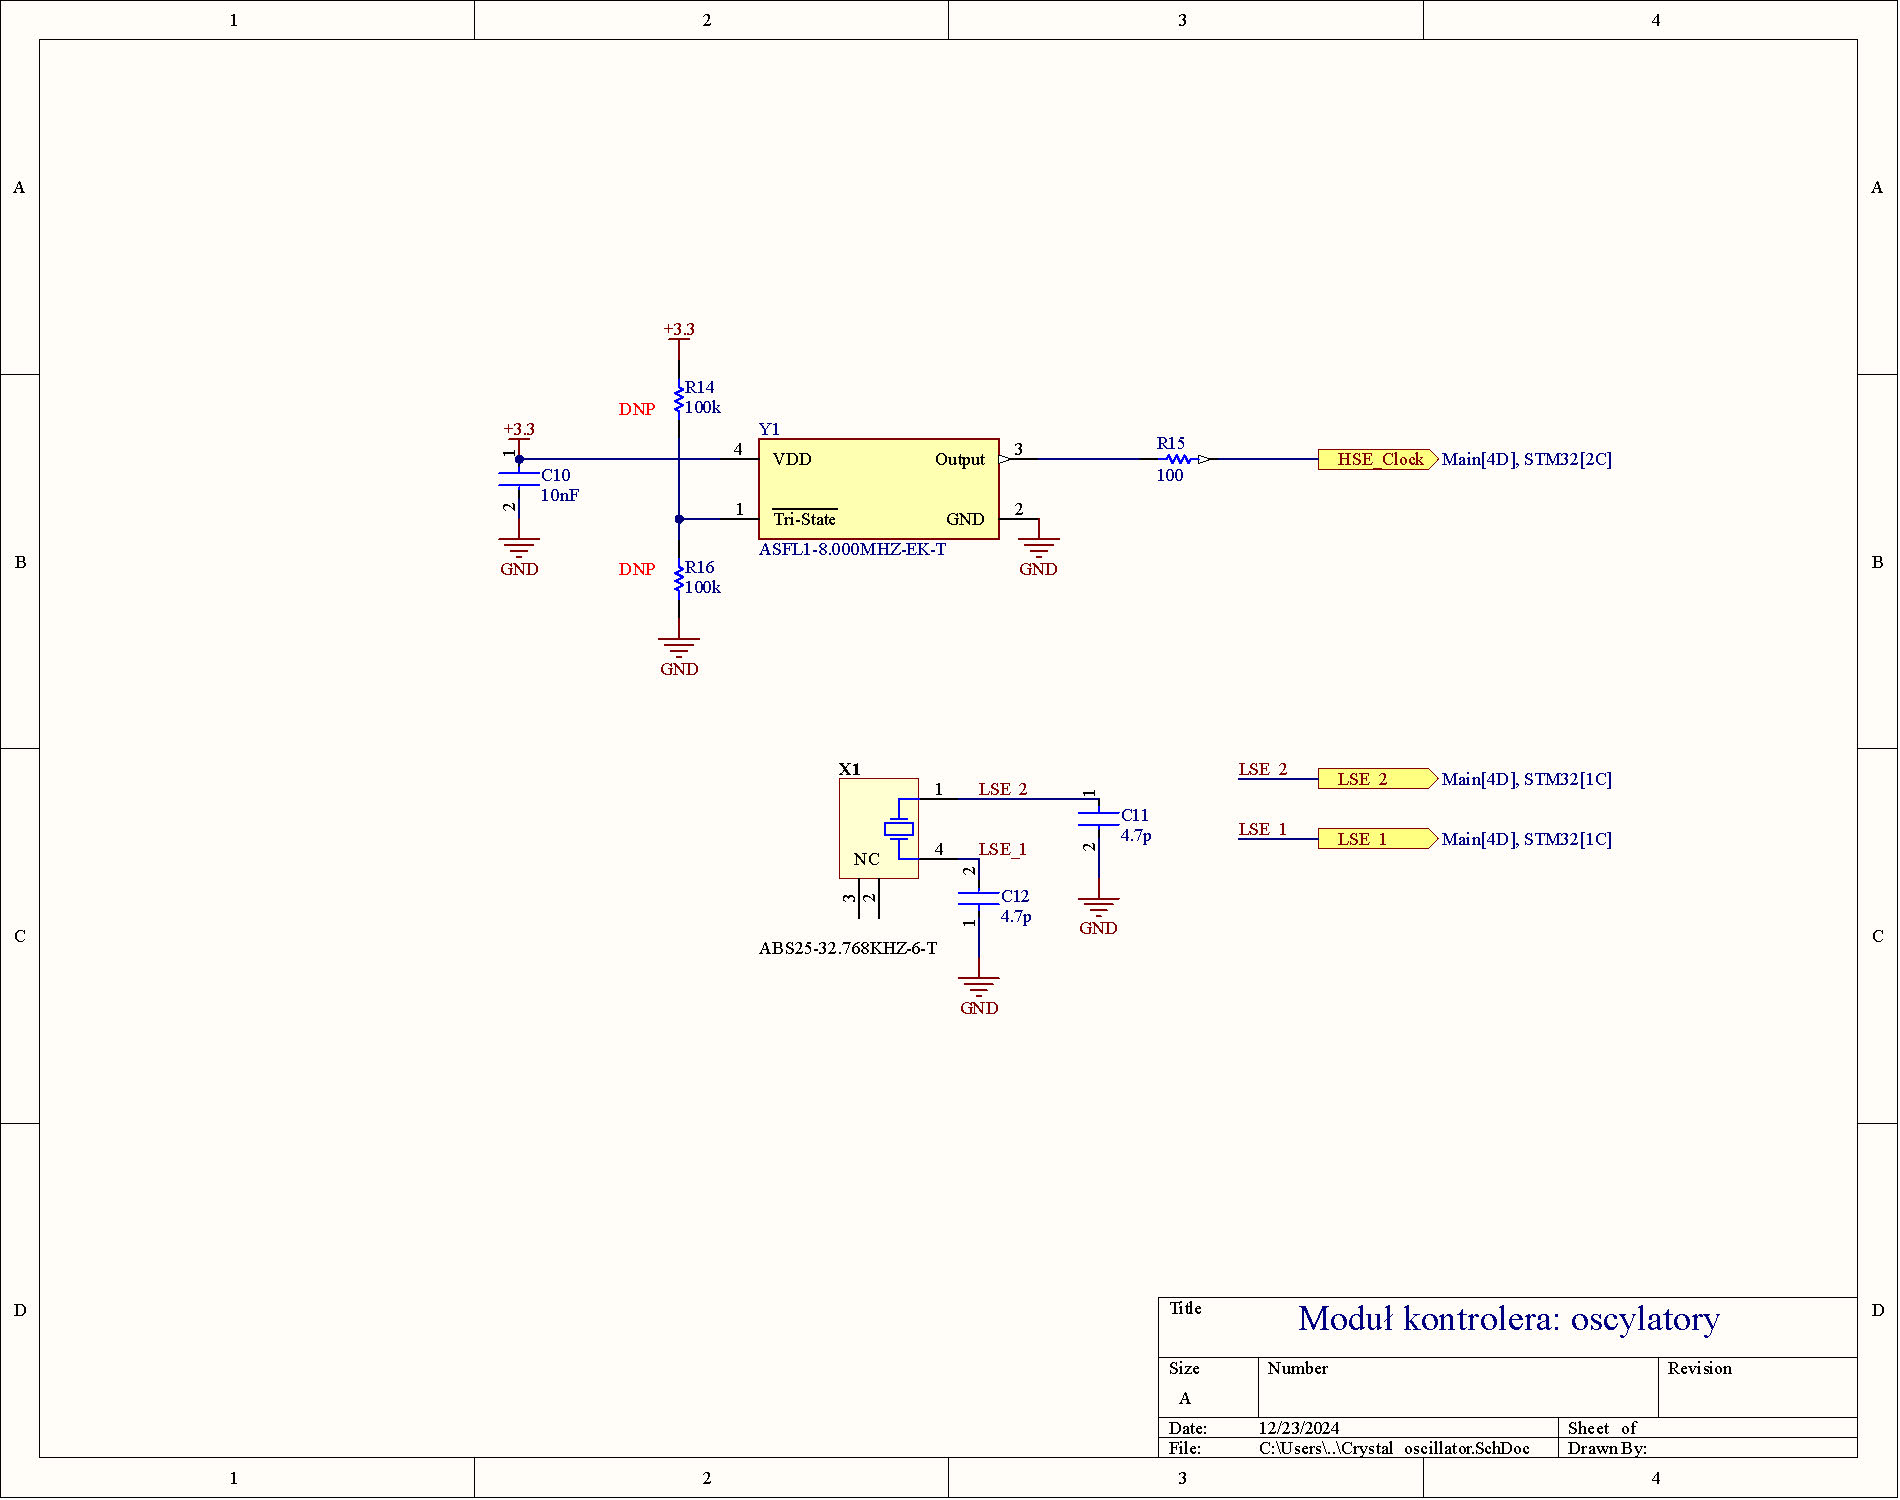
\includegraphics[width = 21cm]{zalaczniki/kontroler/Kontroler_Strona_05.jpg}
        \caption{Schemat układów oscylatorów.}
    \end{center}
\end{sidewaysfigure}

\begin{sidewaysfigure}
    \begin{center}
        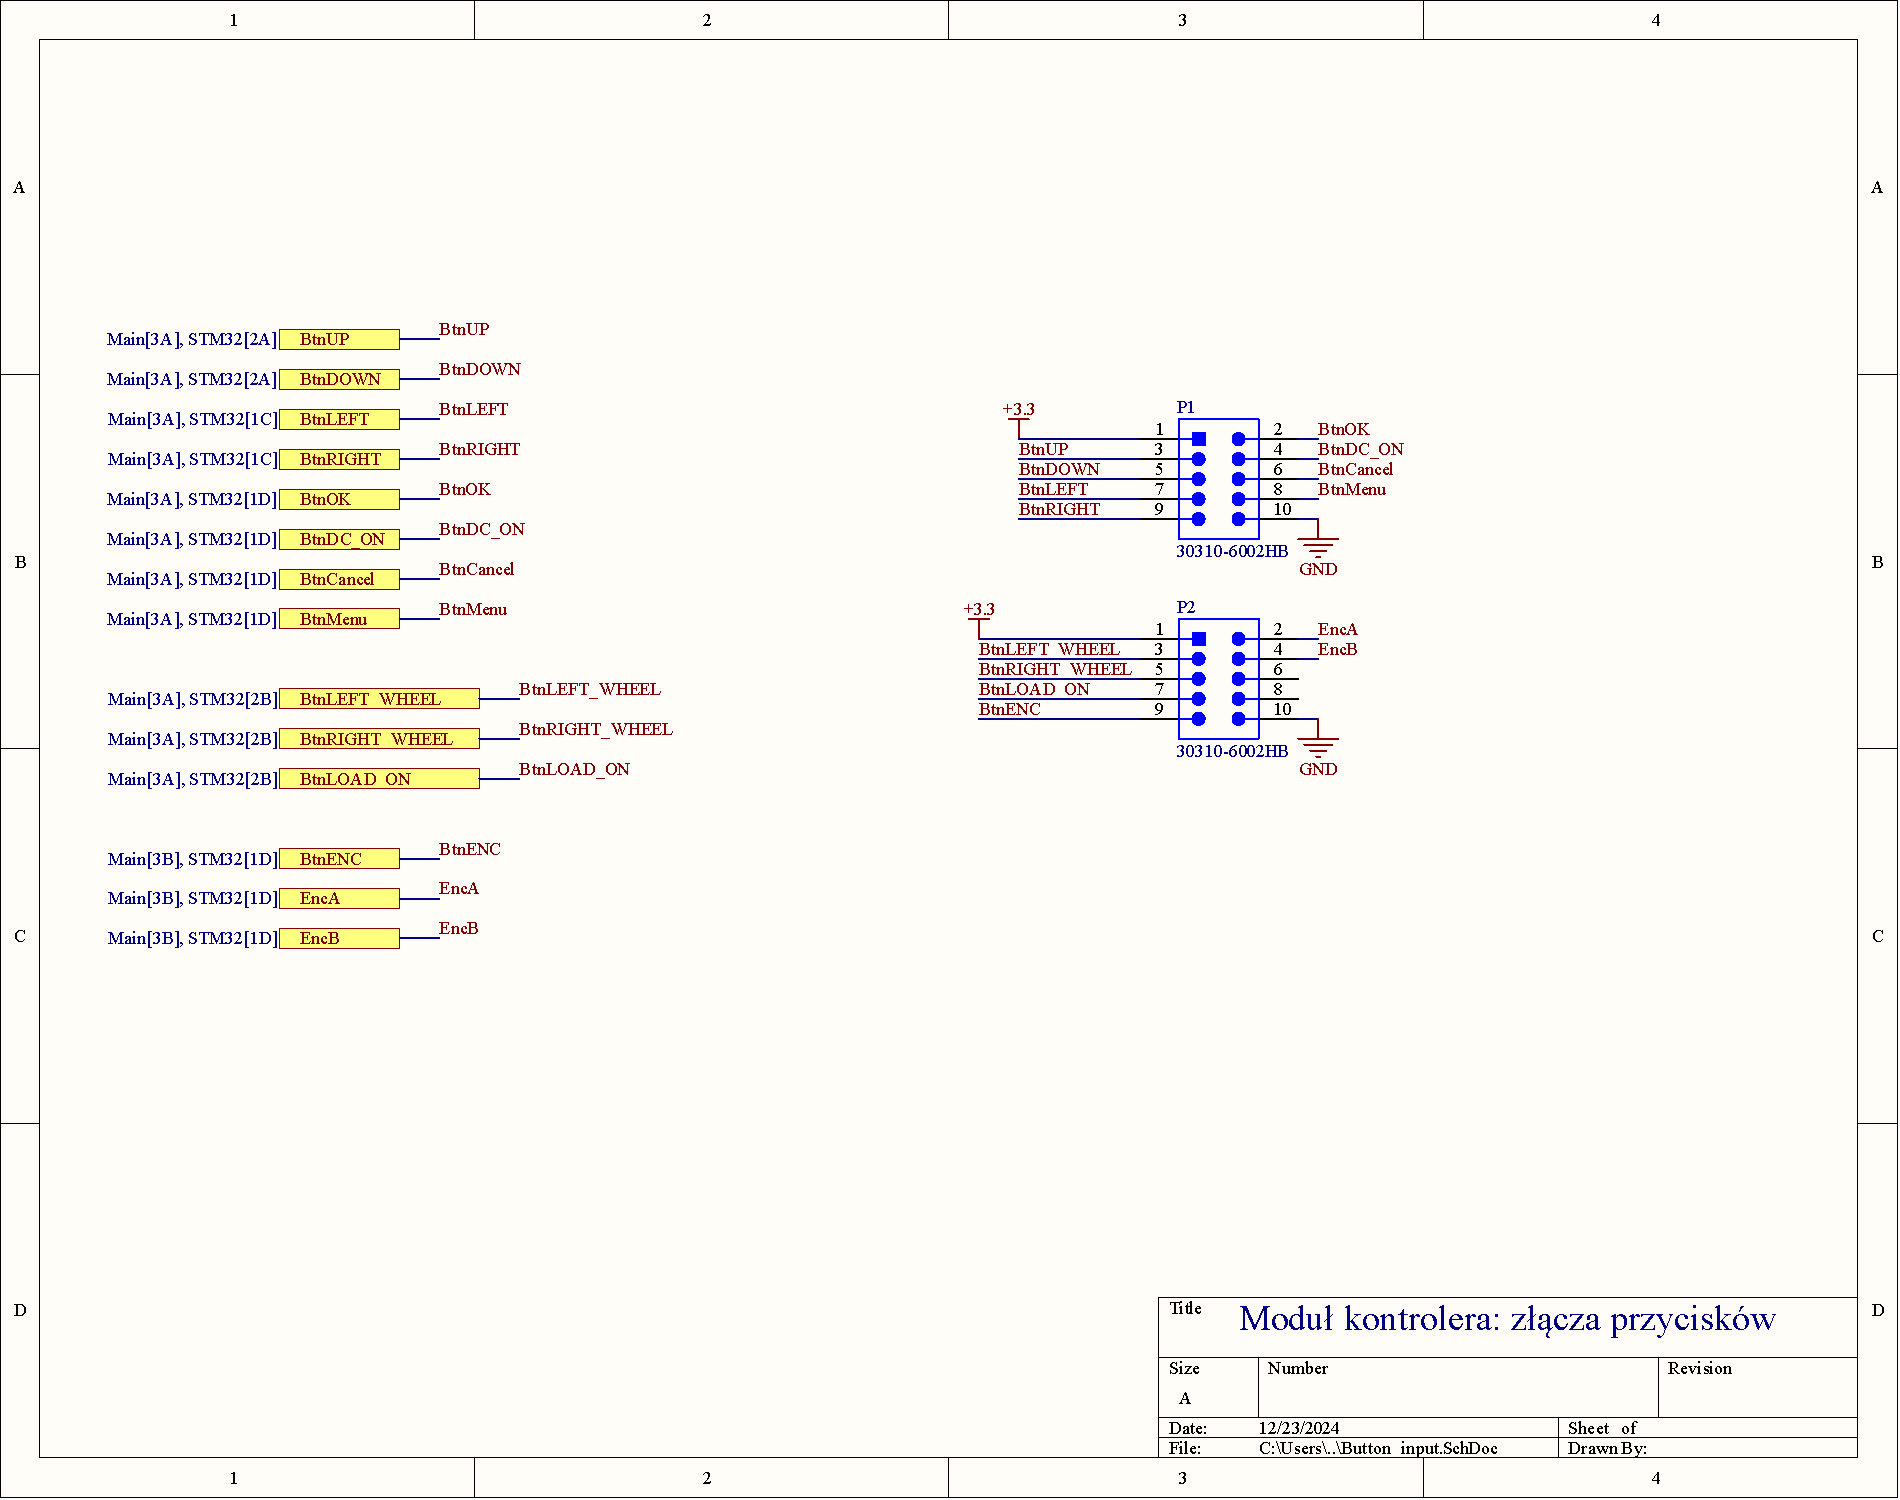
\includegraphics[width = 21cm]{zalaczniki/kontroler/Kontroler_Strona_06.jpg}
        \caption{Schemat wyprowadzeń przycisków.}
    \end{center}
\end{sidewaysfigure}

\begin{sidewaysfigure}
    \begin{center}
        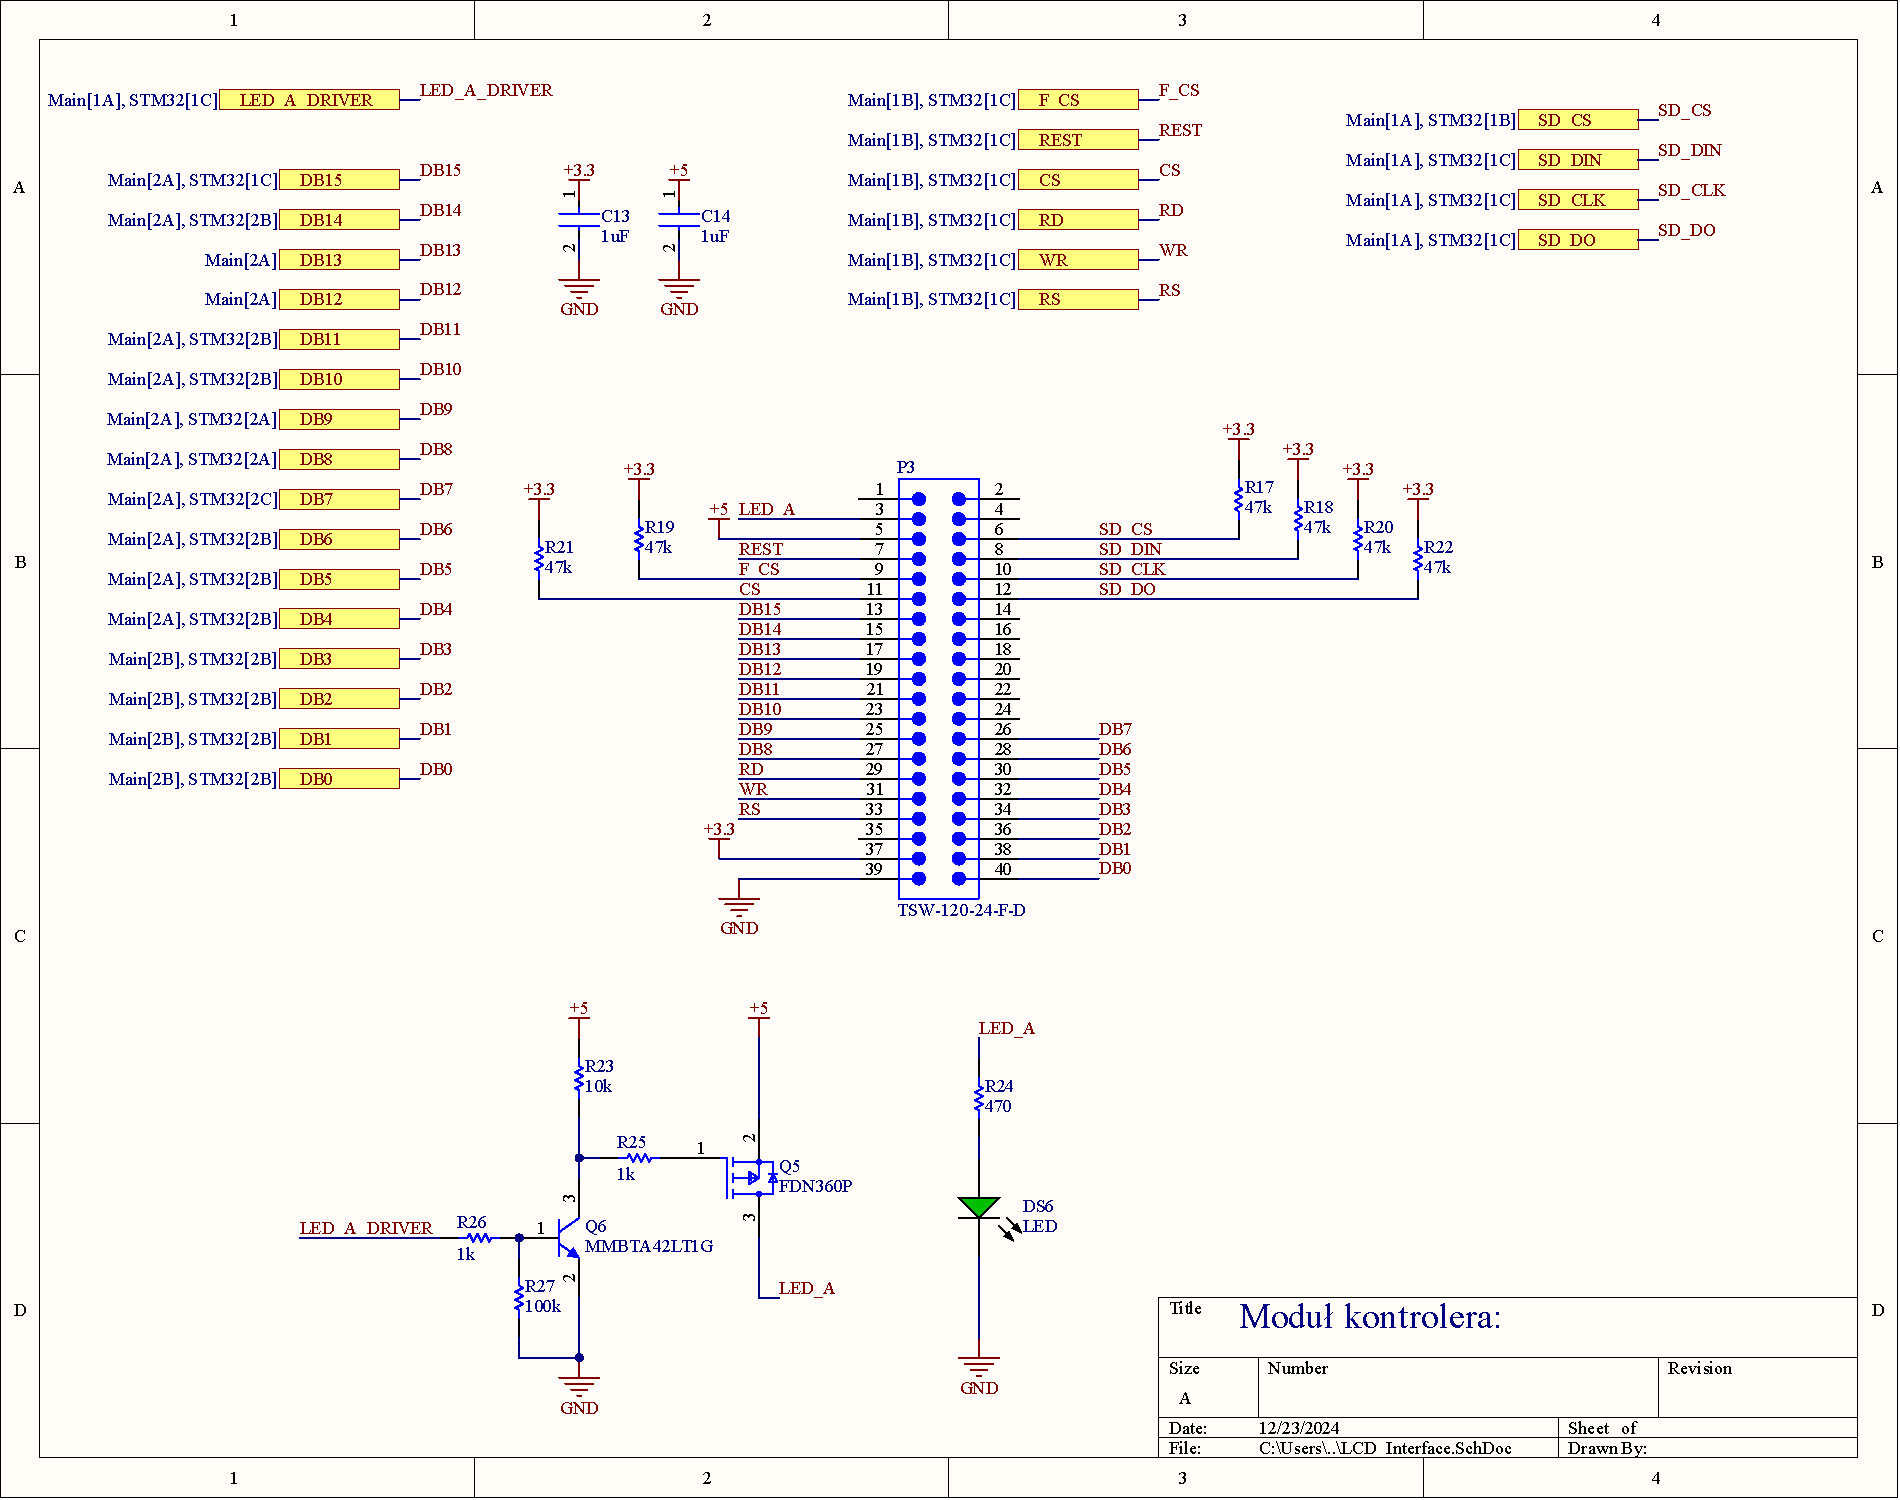
\includegraphics[width = 21cm]{zalaczniki/kontroler/Kontroler_Strona_07.jpg}
        \caption{Schemat wyprowadzania LCD.}
    \end{center}
\end{sidewaysfigure}

\begin{sidewaysfigure}
    \begin{center}
        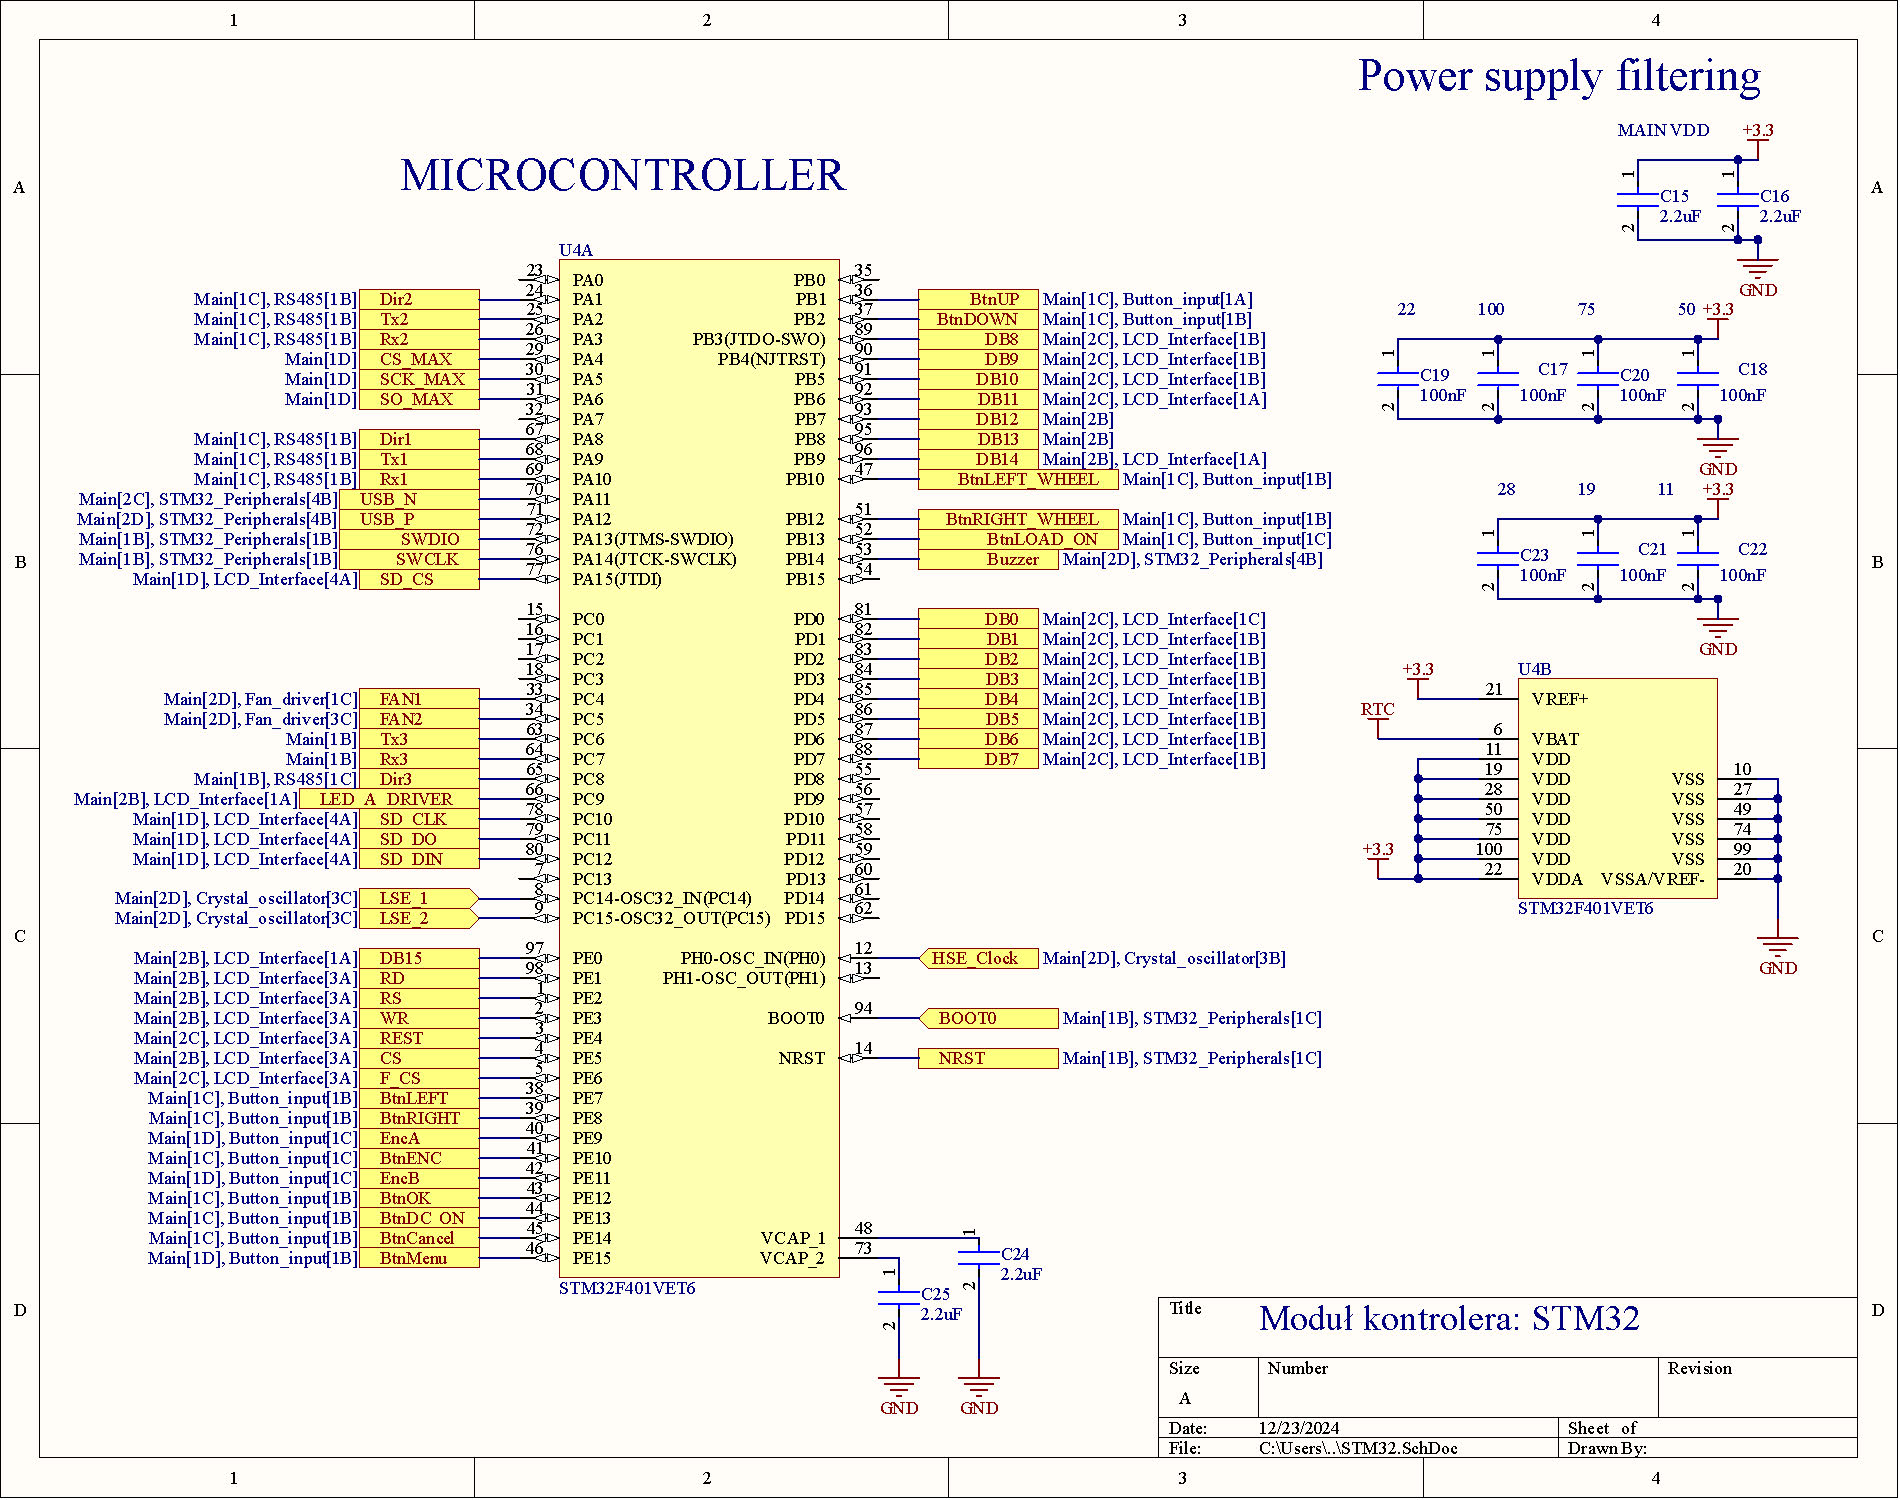
\includegraphics[width = 21cm]{zalaczniki/kontroler/Kontroler_Strona_08.jpg}
        \caption{Schemat mikrokontrolera STM32.}
    \end{center}
\end{sidewaysfigure}

\begin{sidewaysfigure}
    \begin{center}
        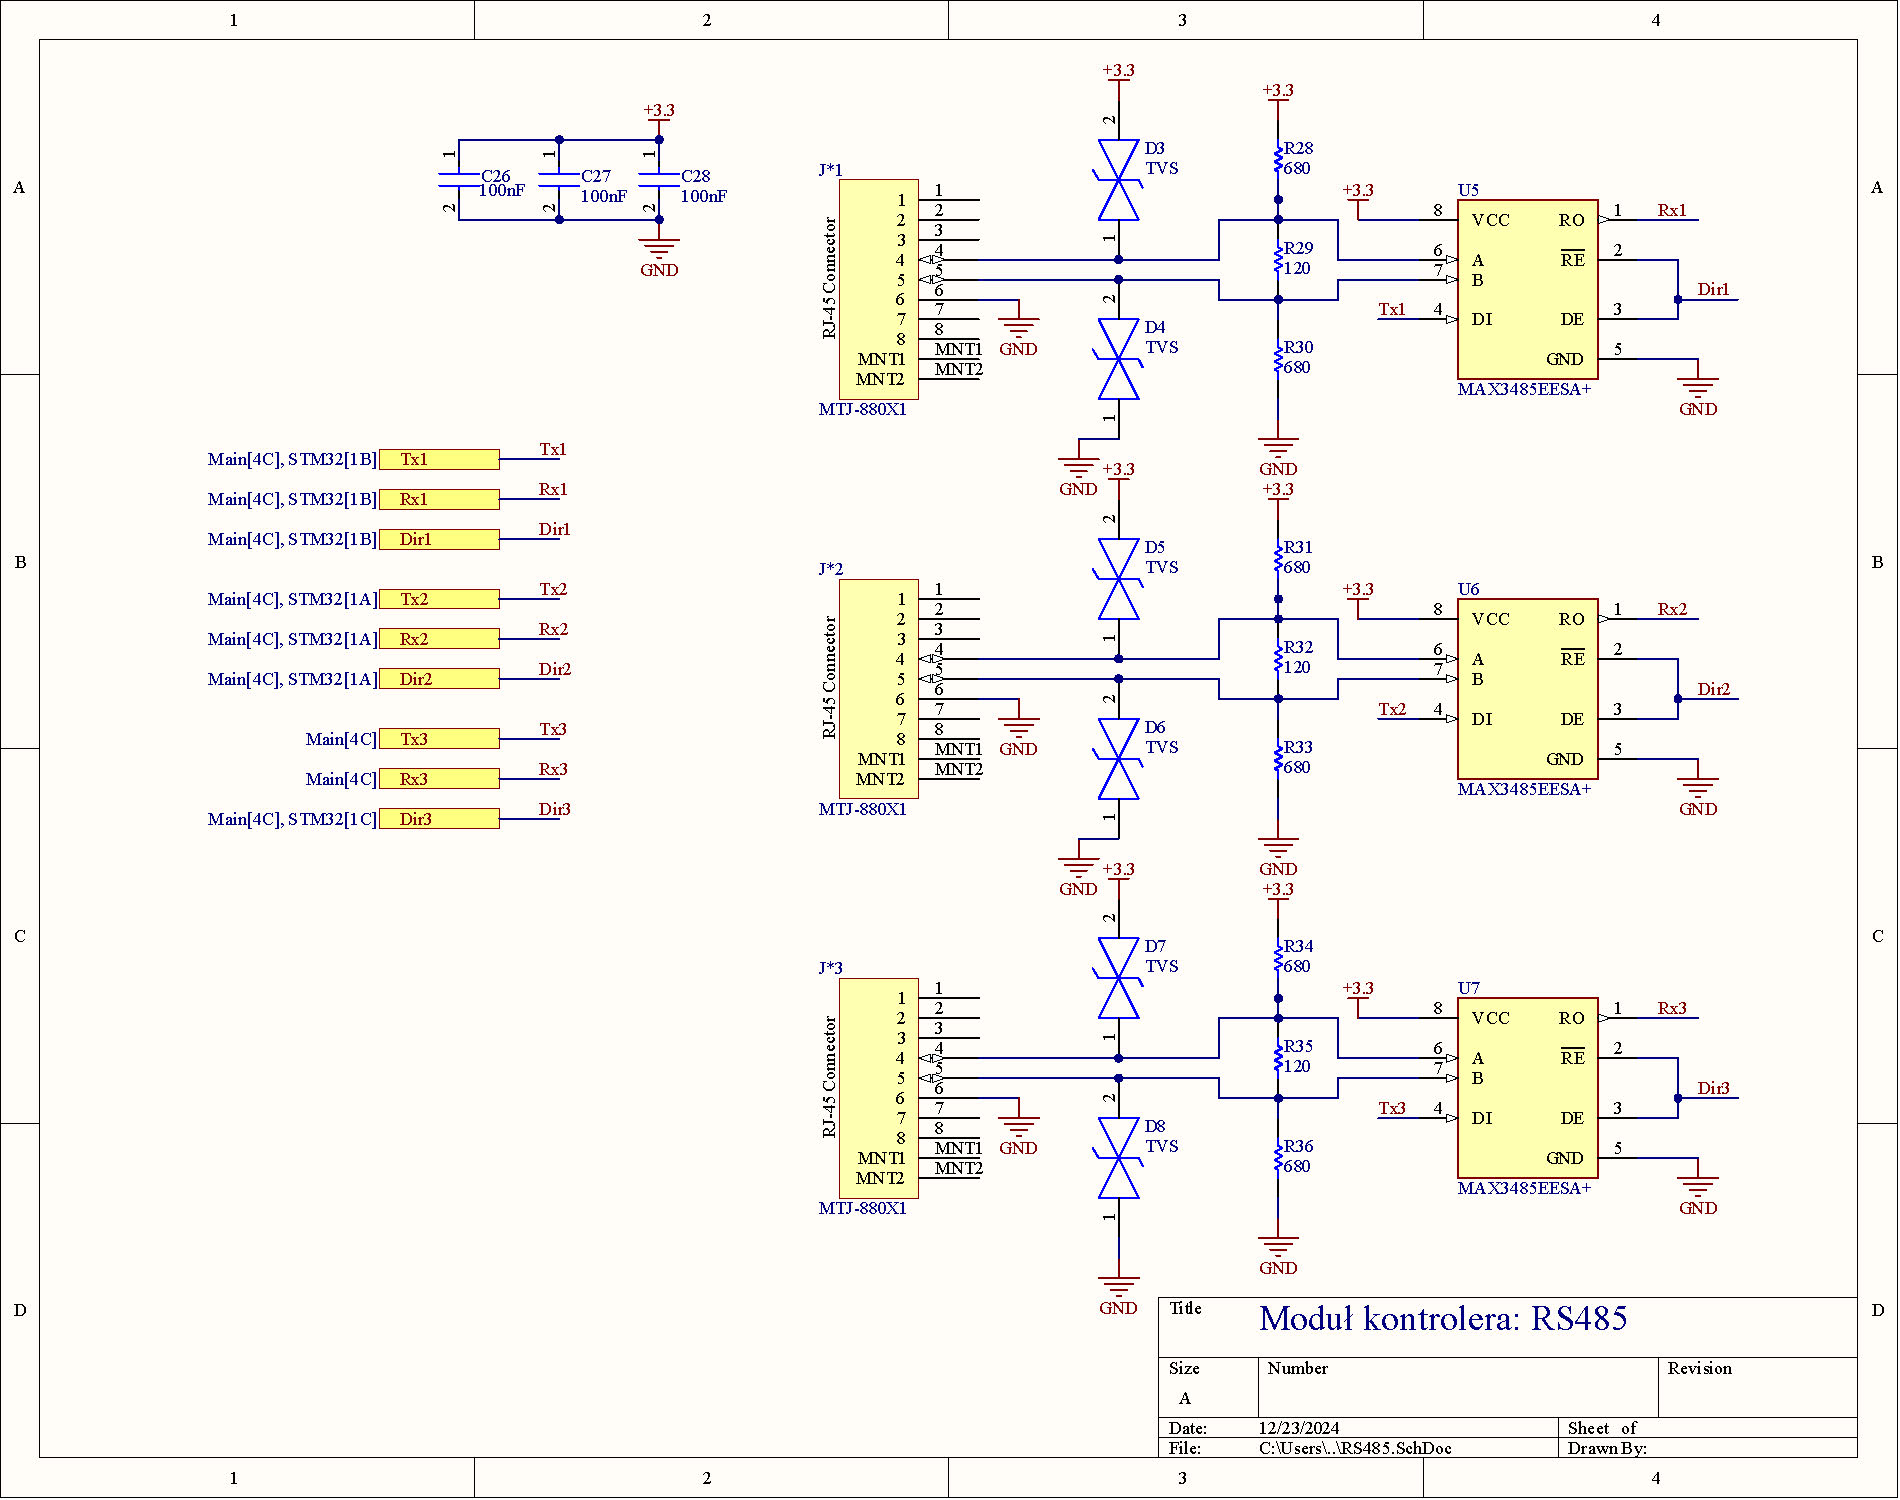
\includegraphics[width = 21cm]{zalaczniki/kontroler/Kontroler_Strona_09.jpg}
        \caption{Schemat RS485.}
    \end{center}
\end{sidewaysfigure}

\begin{sidewaysfigure}
    \begin{center}
        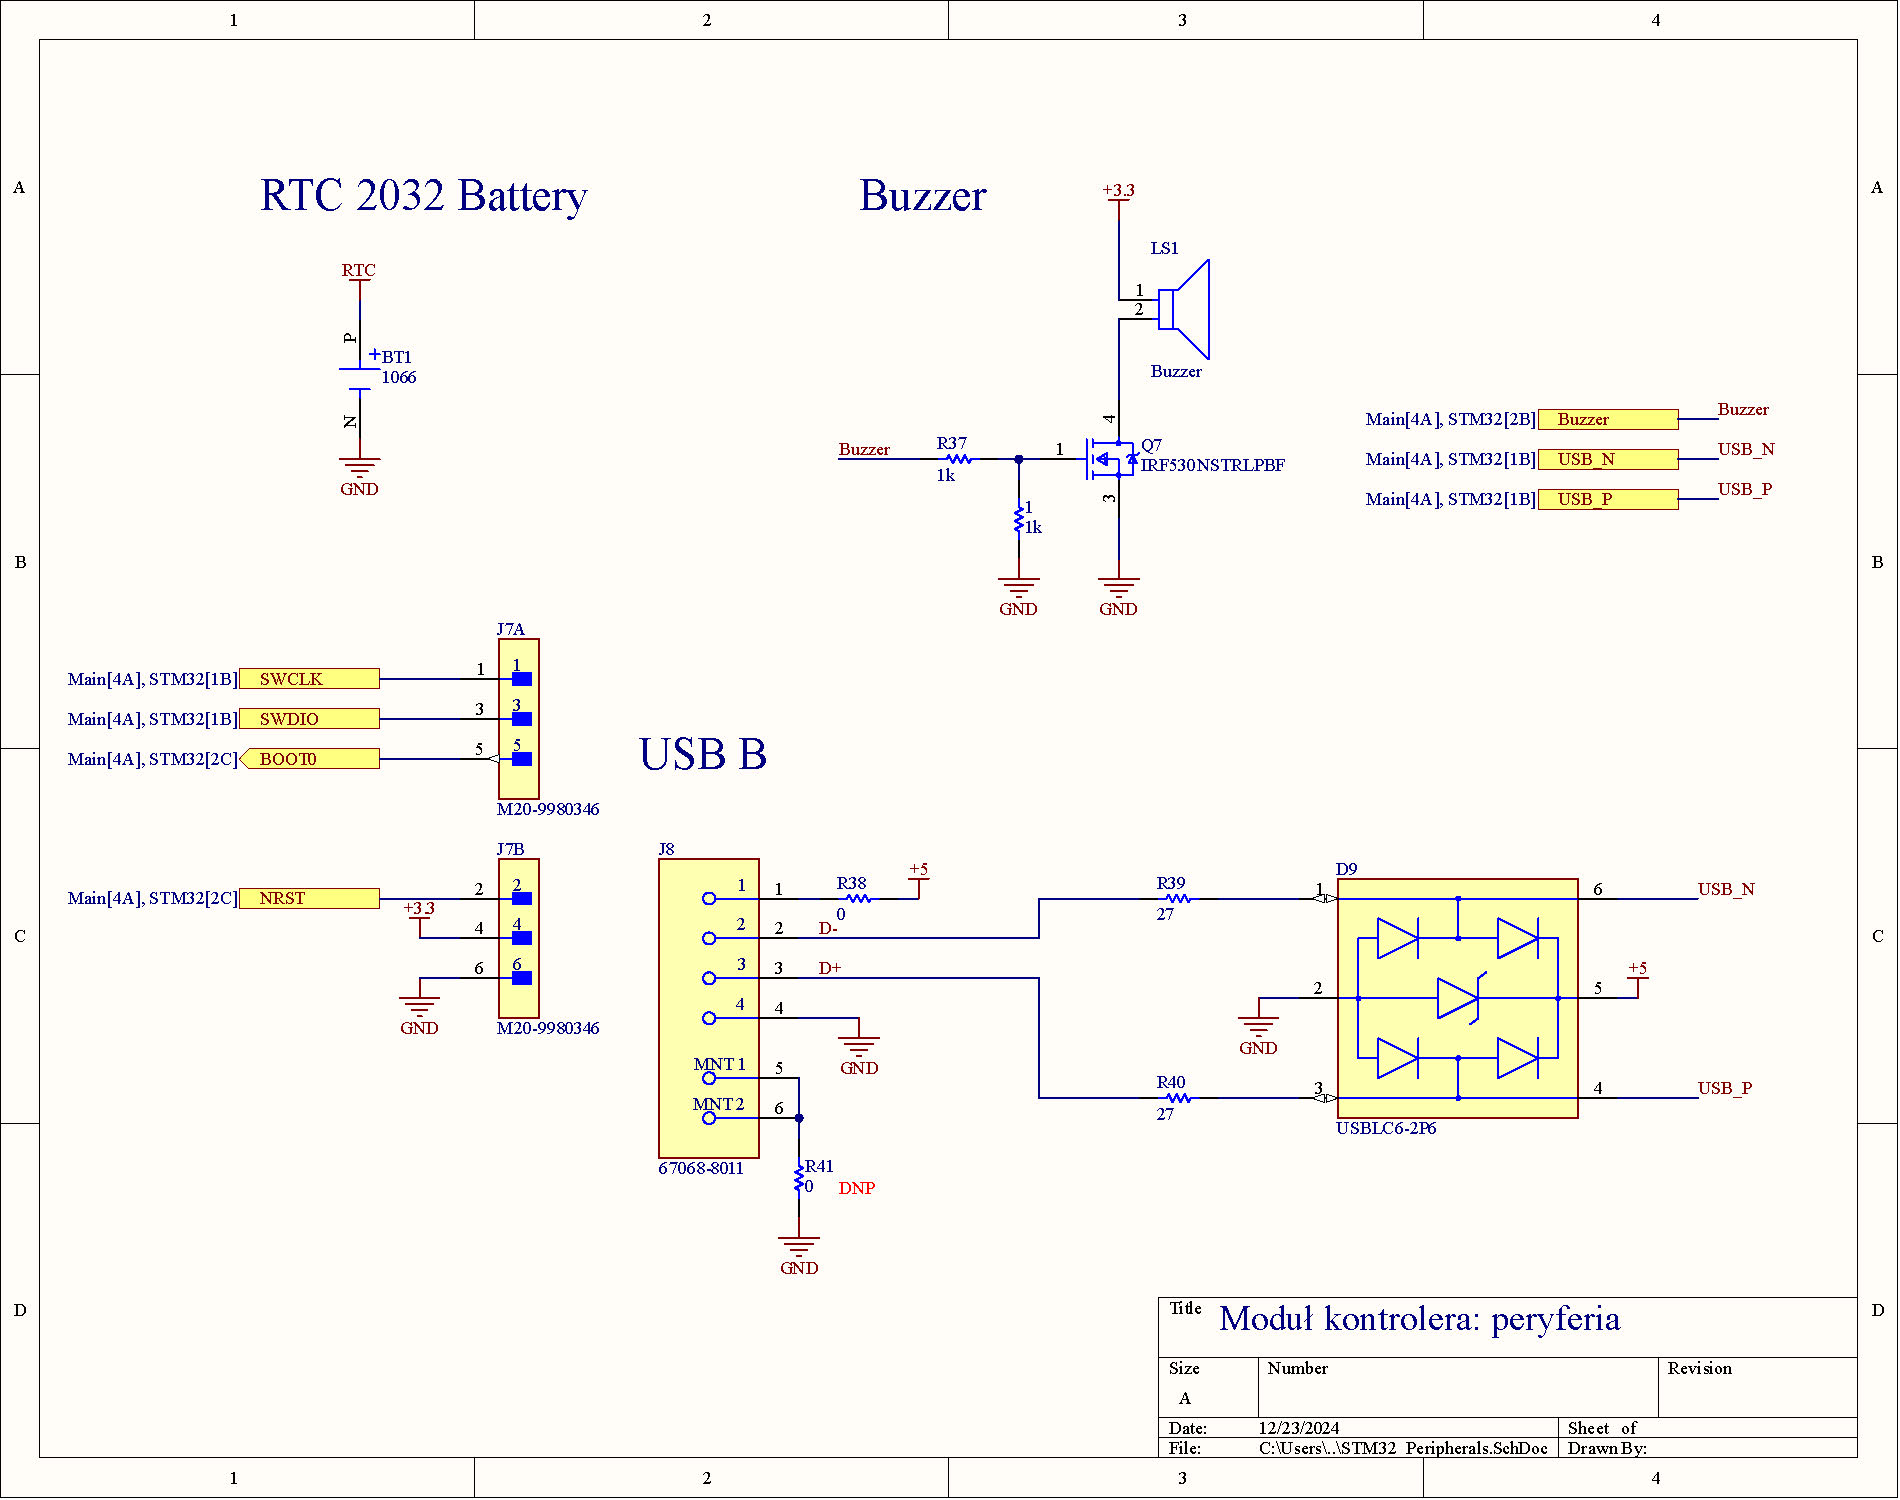
\includegraphics[width = 21cm]{zalaczniki/kontroler/Kontroler_Strona_10.jpg}
        \caption{Schemat układów peryferyjnych.}
    \end{center}
\end{sidewaysfigure}

\begin{figure}
    \begin{center}
        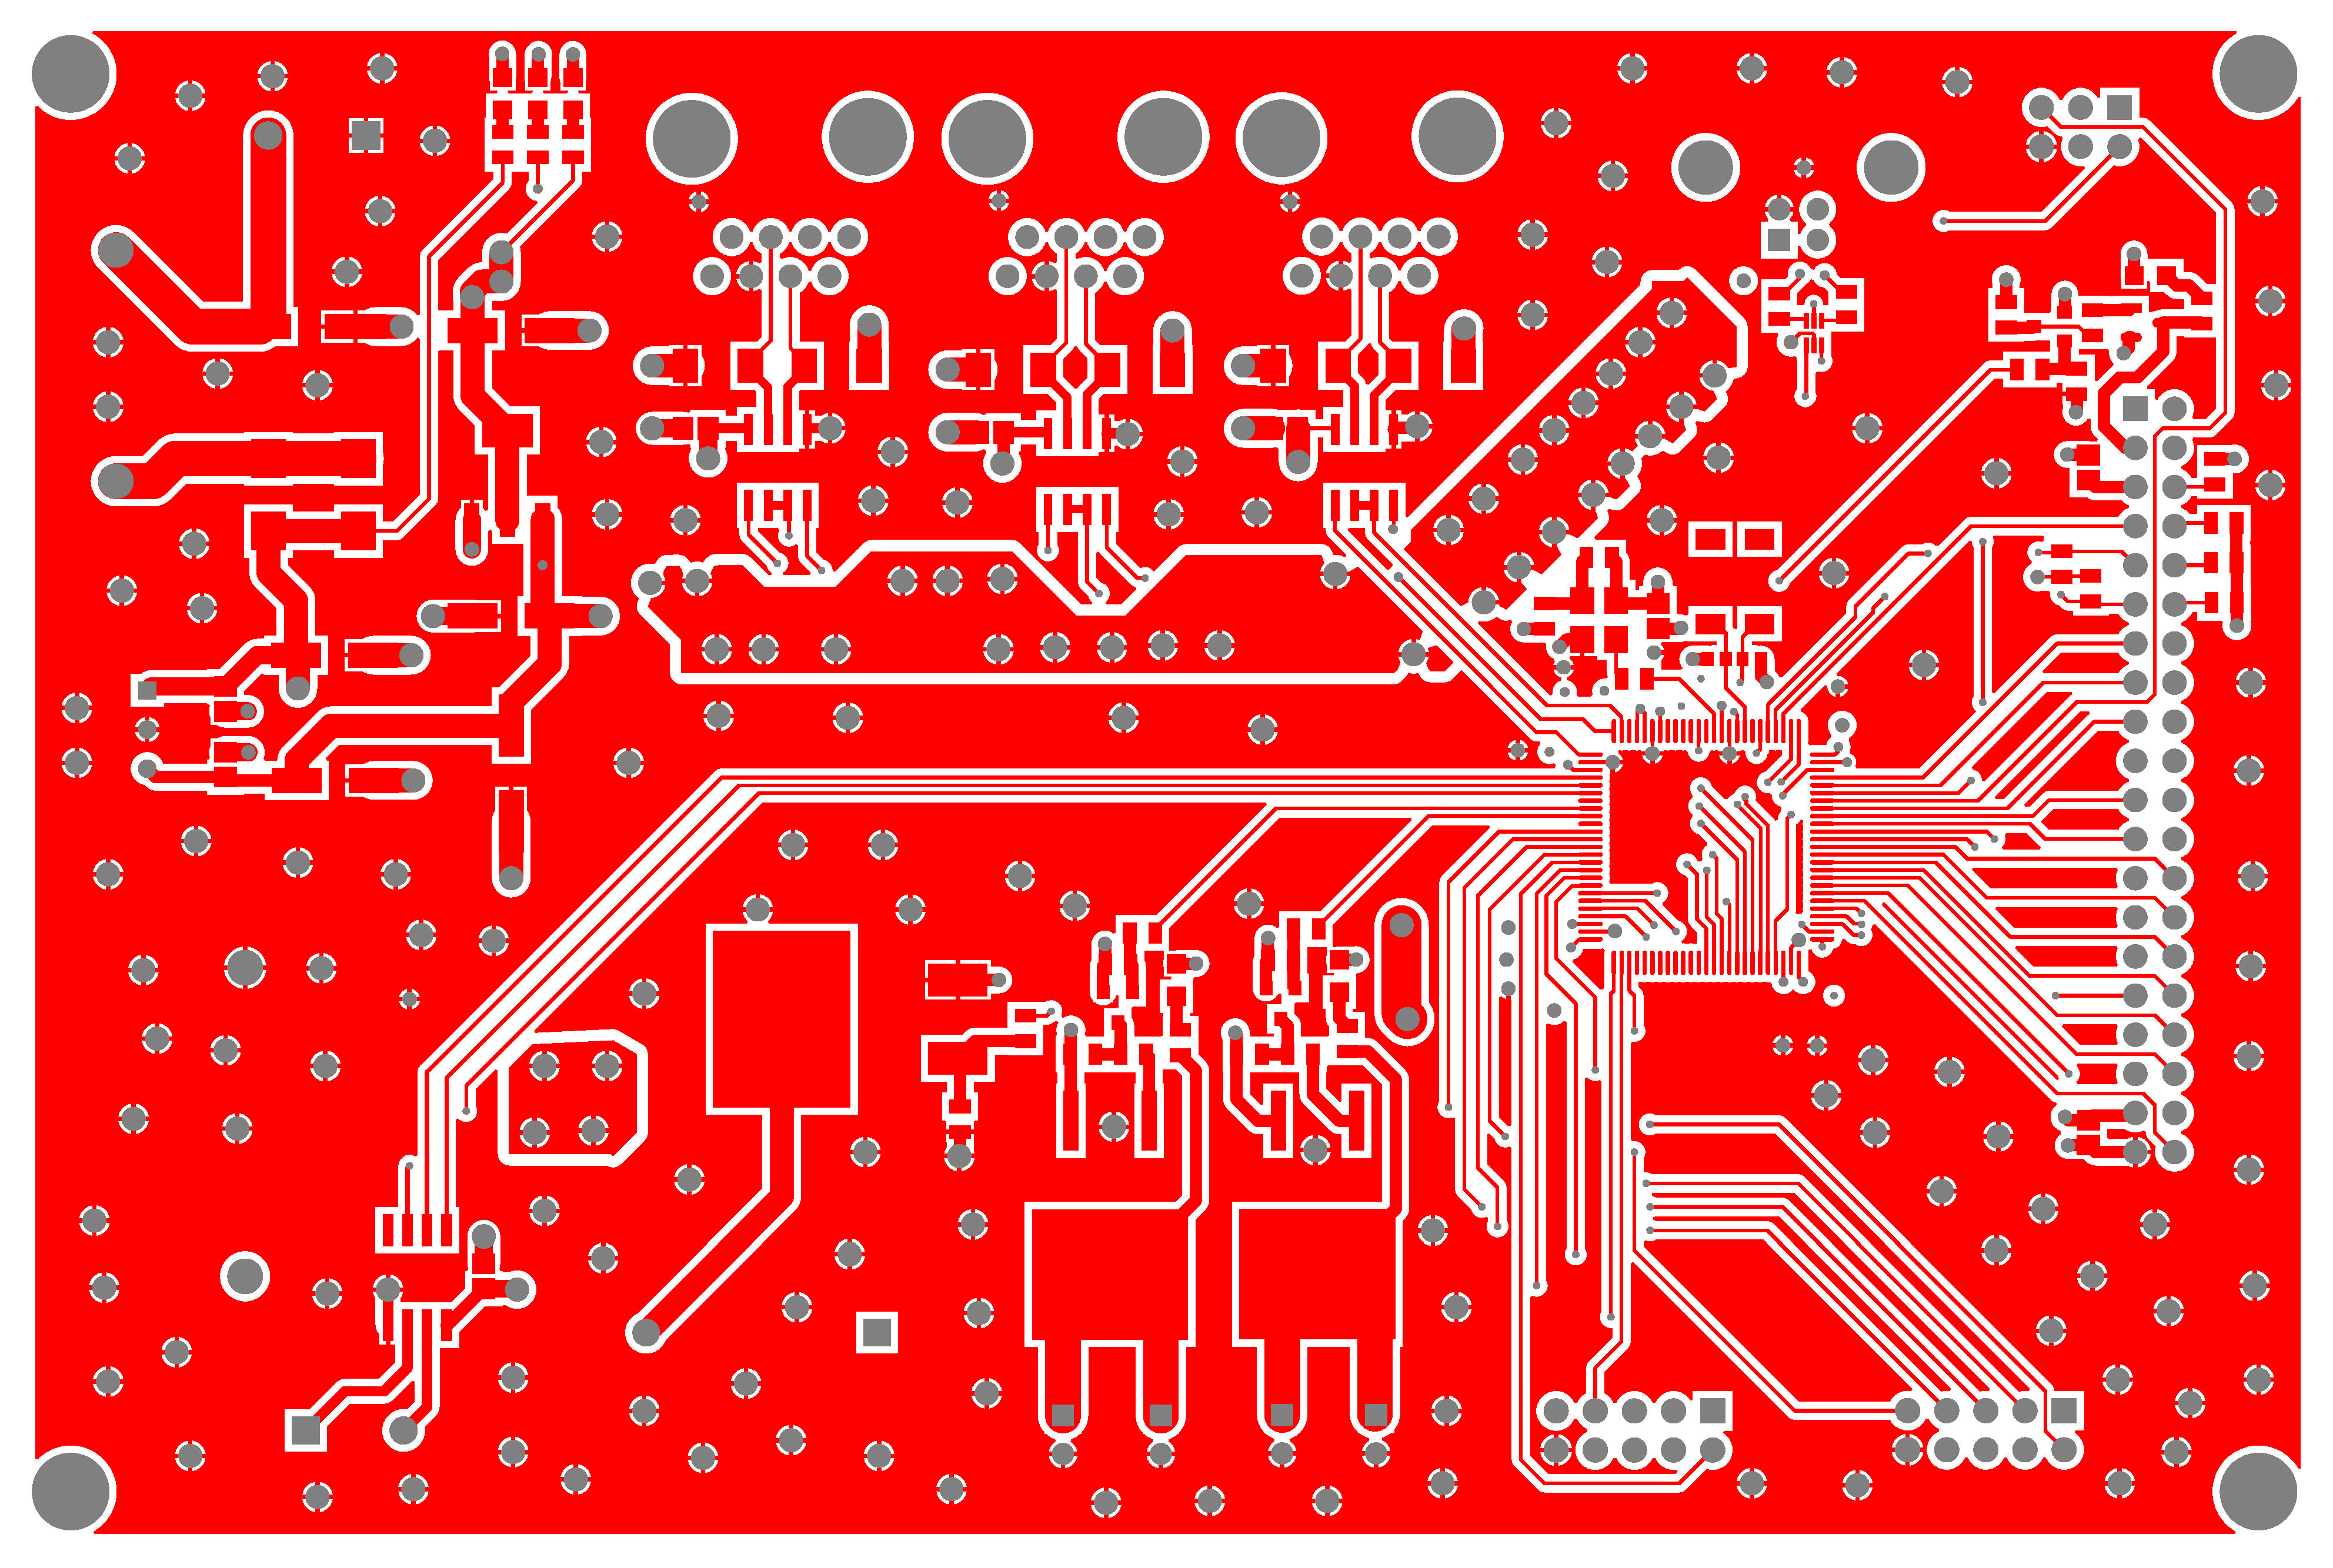
\includegraphics[width = 15cm]{zalaczniki/kontroler/Kontroler_Strona_11.jpg}
        \caption{Warstwa górna PCB.}
    \end{center}
\end{figure}

\begin{figure}
    \begin{center}
        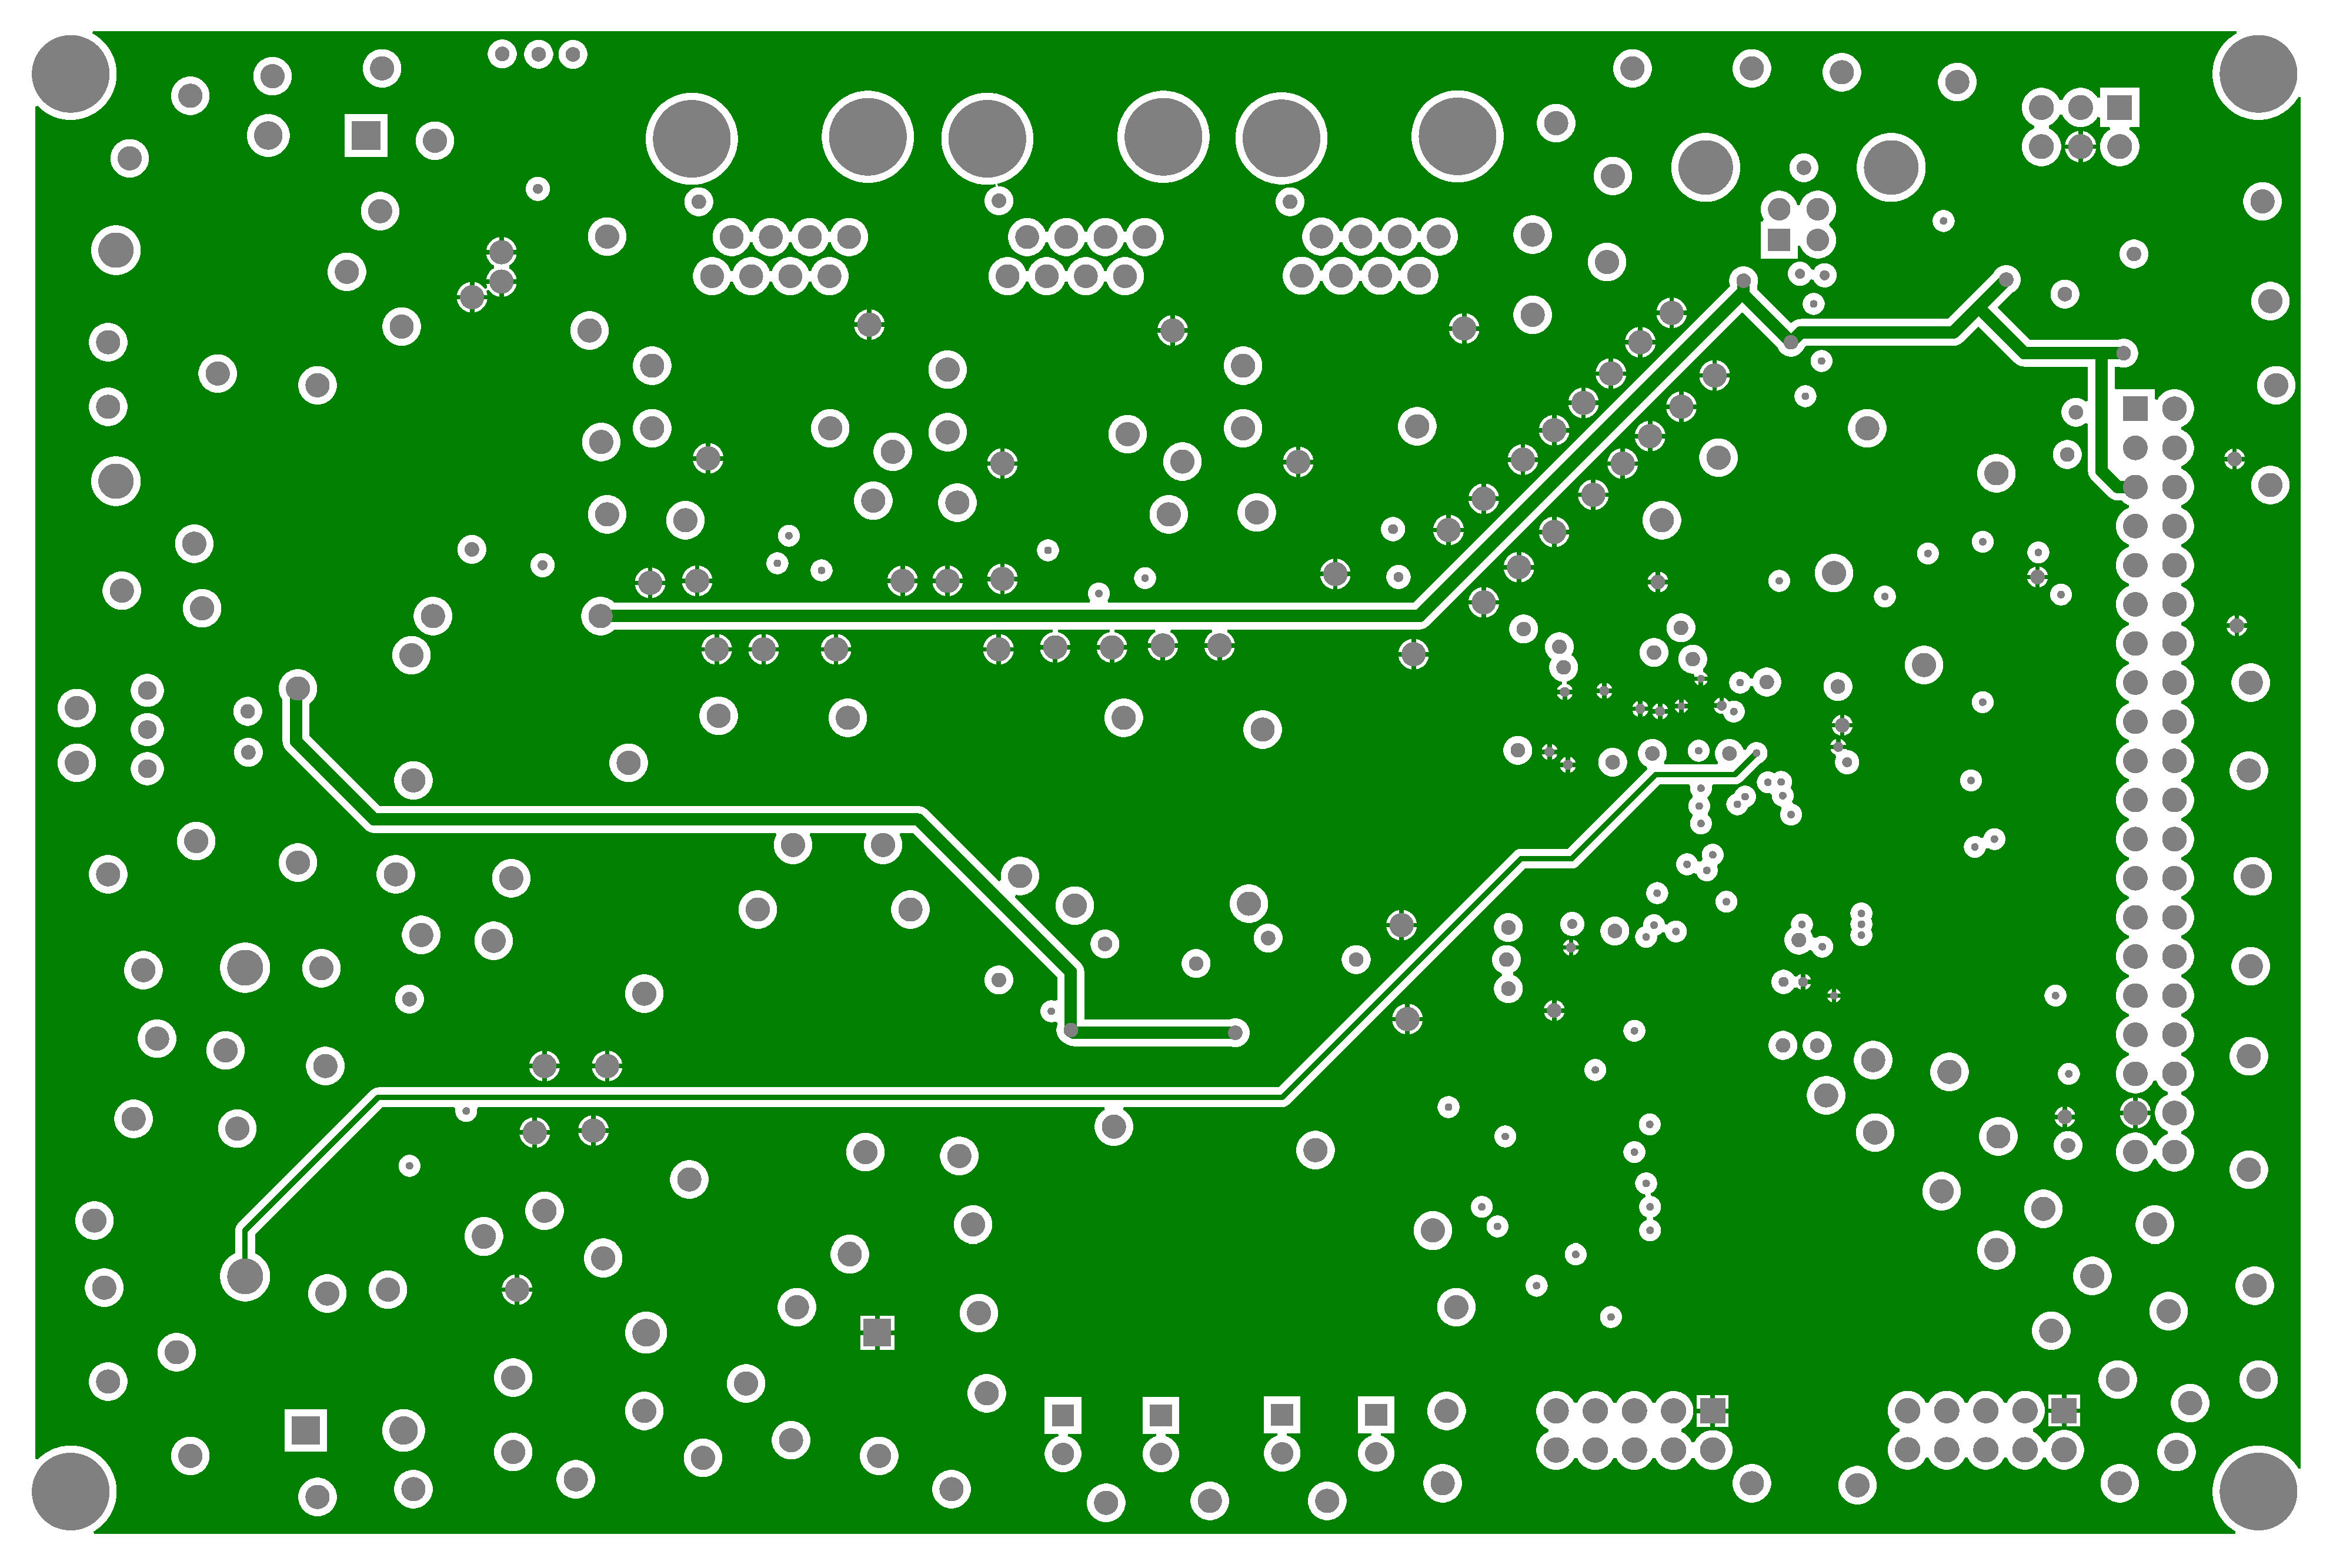
\includegraphics[width = 15cm]{zalaczniki/kontroler/Kontroler_Strona_12.jpg}
        \caption{Warstwa wewnętrzna 1 PCB.}
    \end{center}
\end{figure}

\begin{figure}
    \begin{center}
        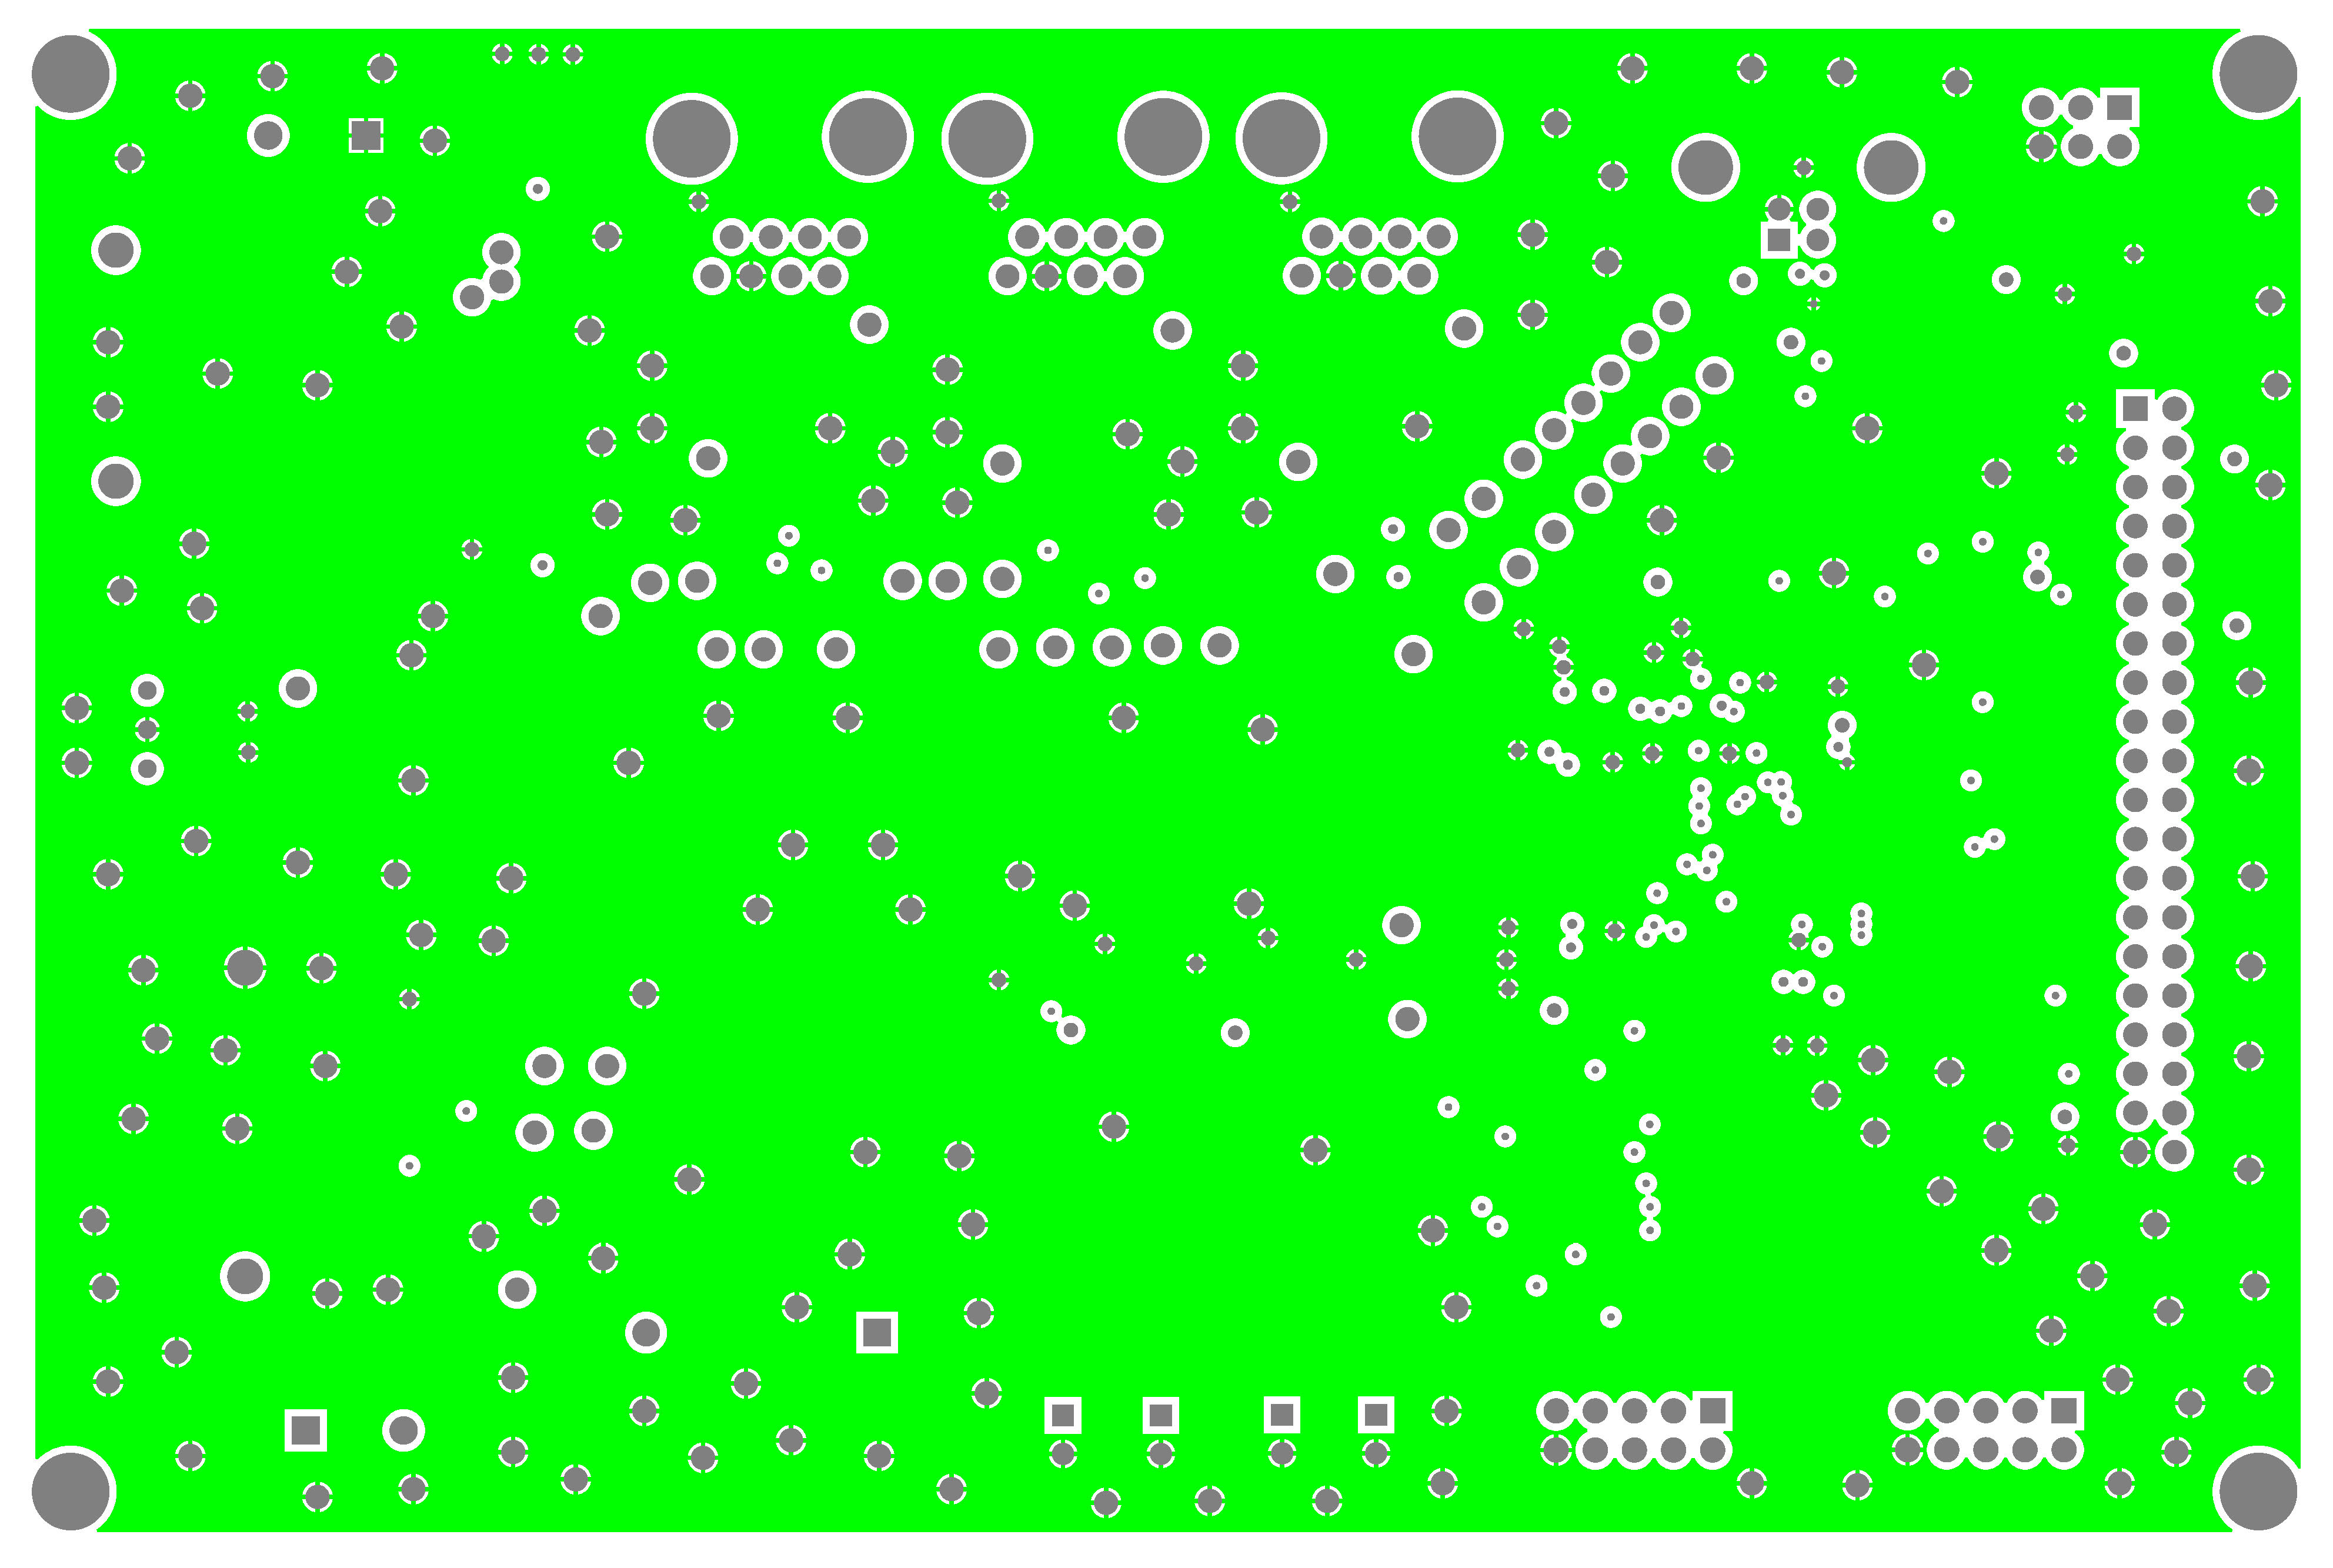
\includegraphics[width = 15cm]{zalaczniki/kontroler/Kontroler_Strona_13.jpg}
        \caption{Warstwa wewnętrzna 2 PCB.}
    \end{center}
\end{figure}

\begin{figure}
    \begin{center}
        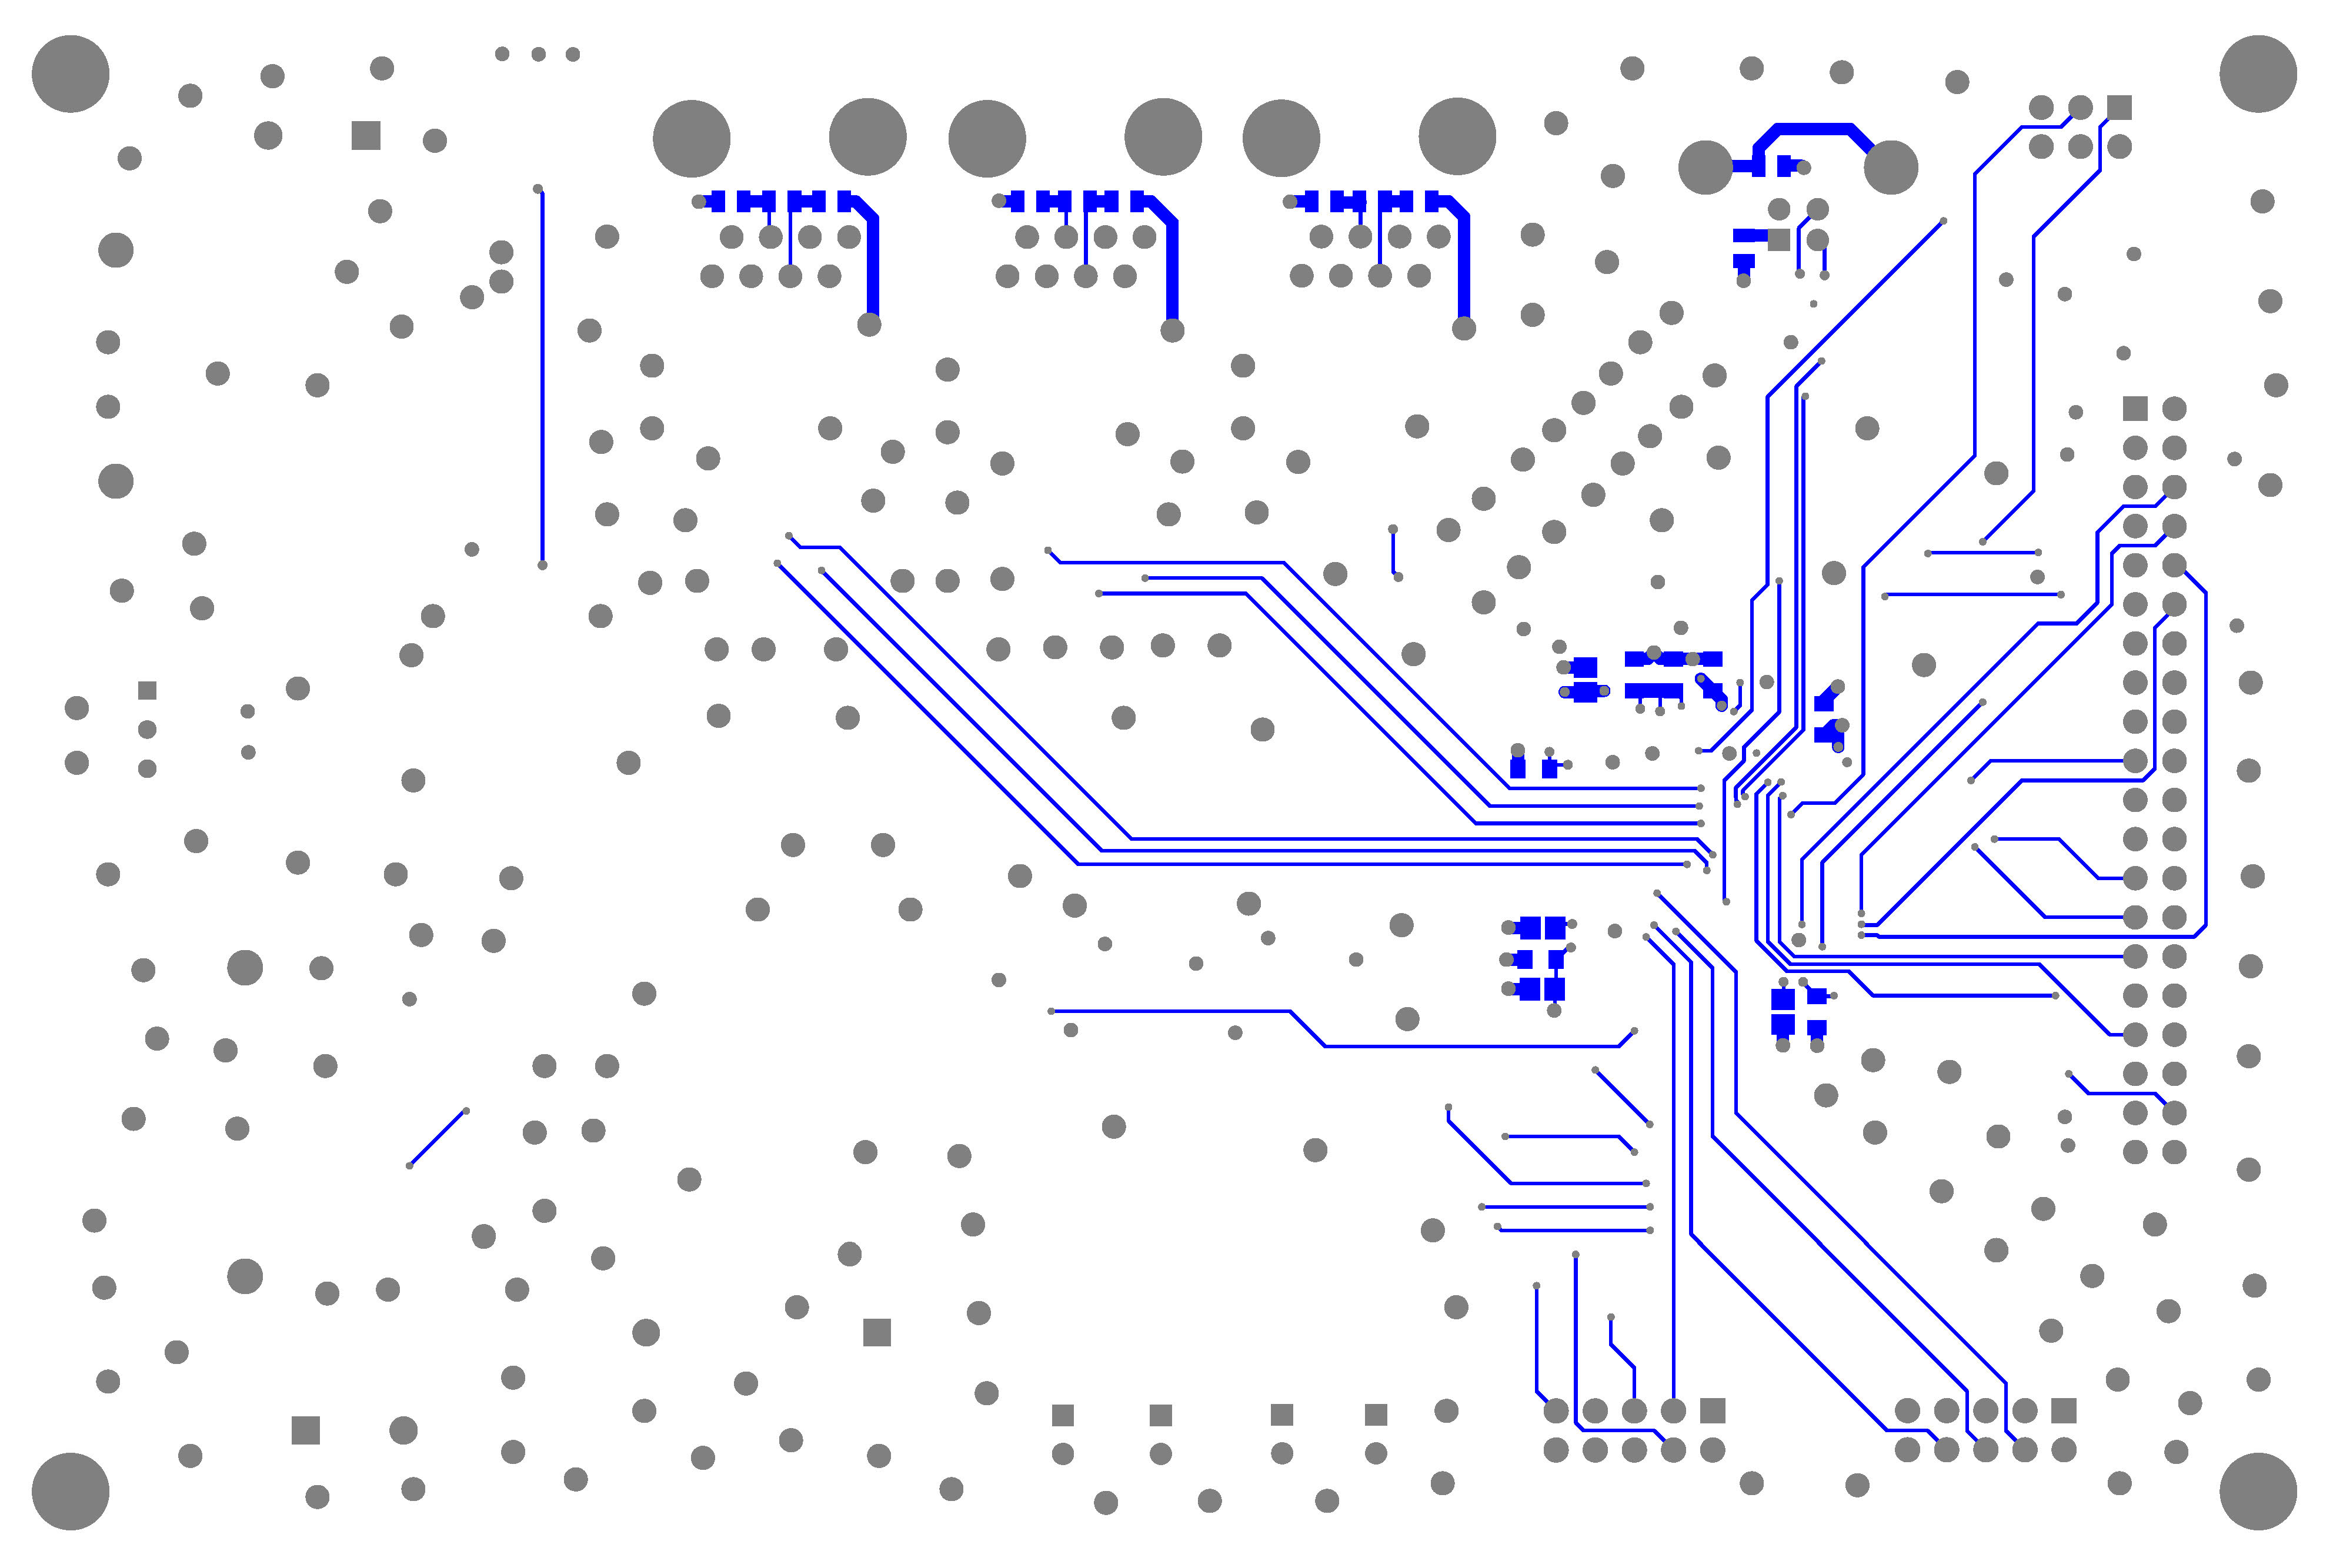
\includegraphics[width = 15cm]{zalaczniki/kontroler/Kontroler_Strona_14.jpg}
        \caption{Warstwa dolna PCB.}
    \end{center}
\end{figure}



\nopagebreak

\chapter{Moduł zasilacza regulowanego}


\begin{figure}[h!]
    \begin{center}
        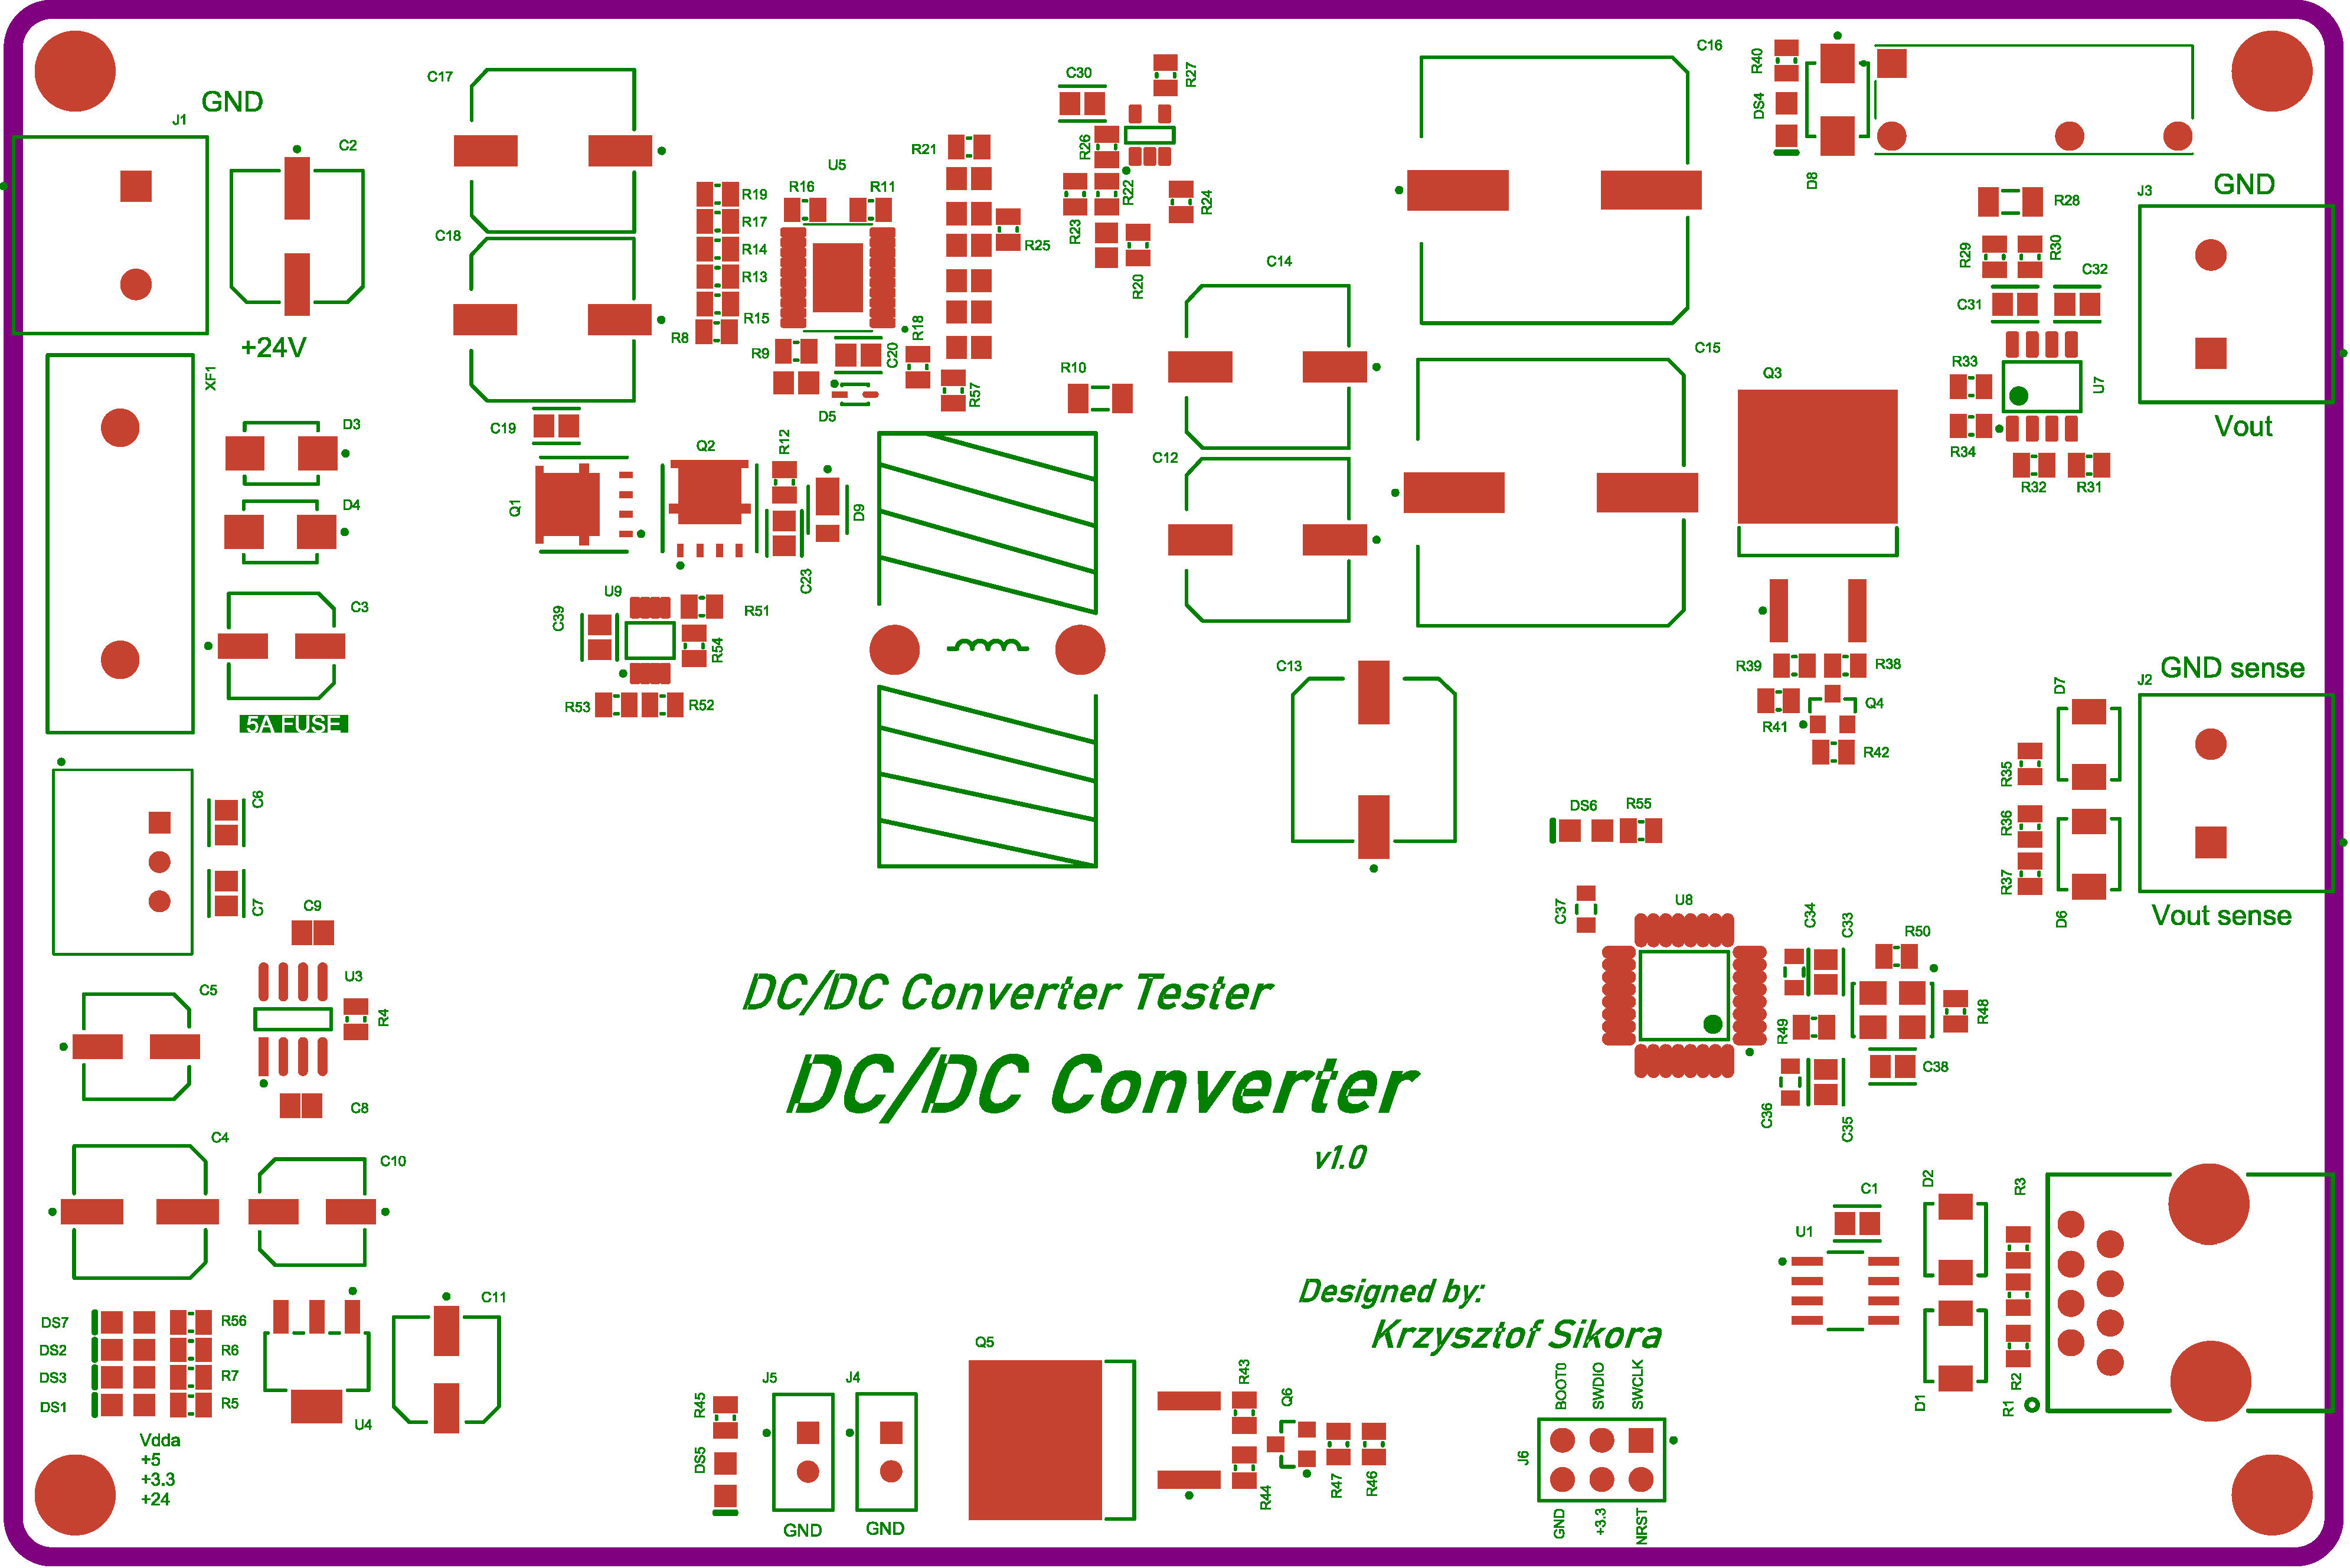
\includegraphics[width = 17cm]{zalaczniki/zasilacz/Zasilacz_regulowany_Strona_13.jpg}
        \caption{Widok warstwy opisowej PCB.}
    \end{center}
\end{figure}

\begin{sidewaysfigure}
    \begin{center}
        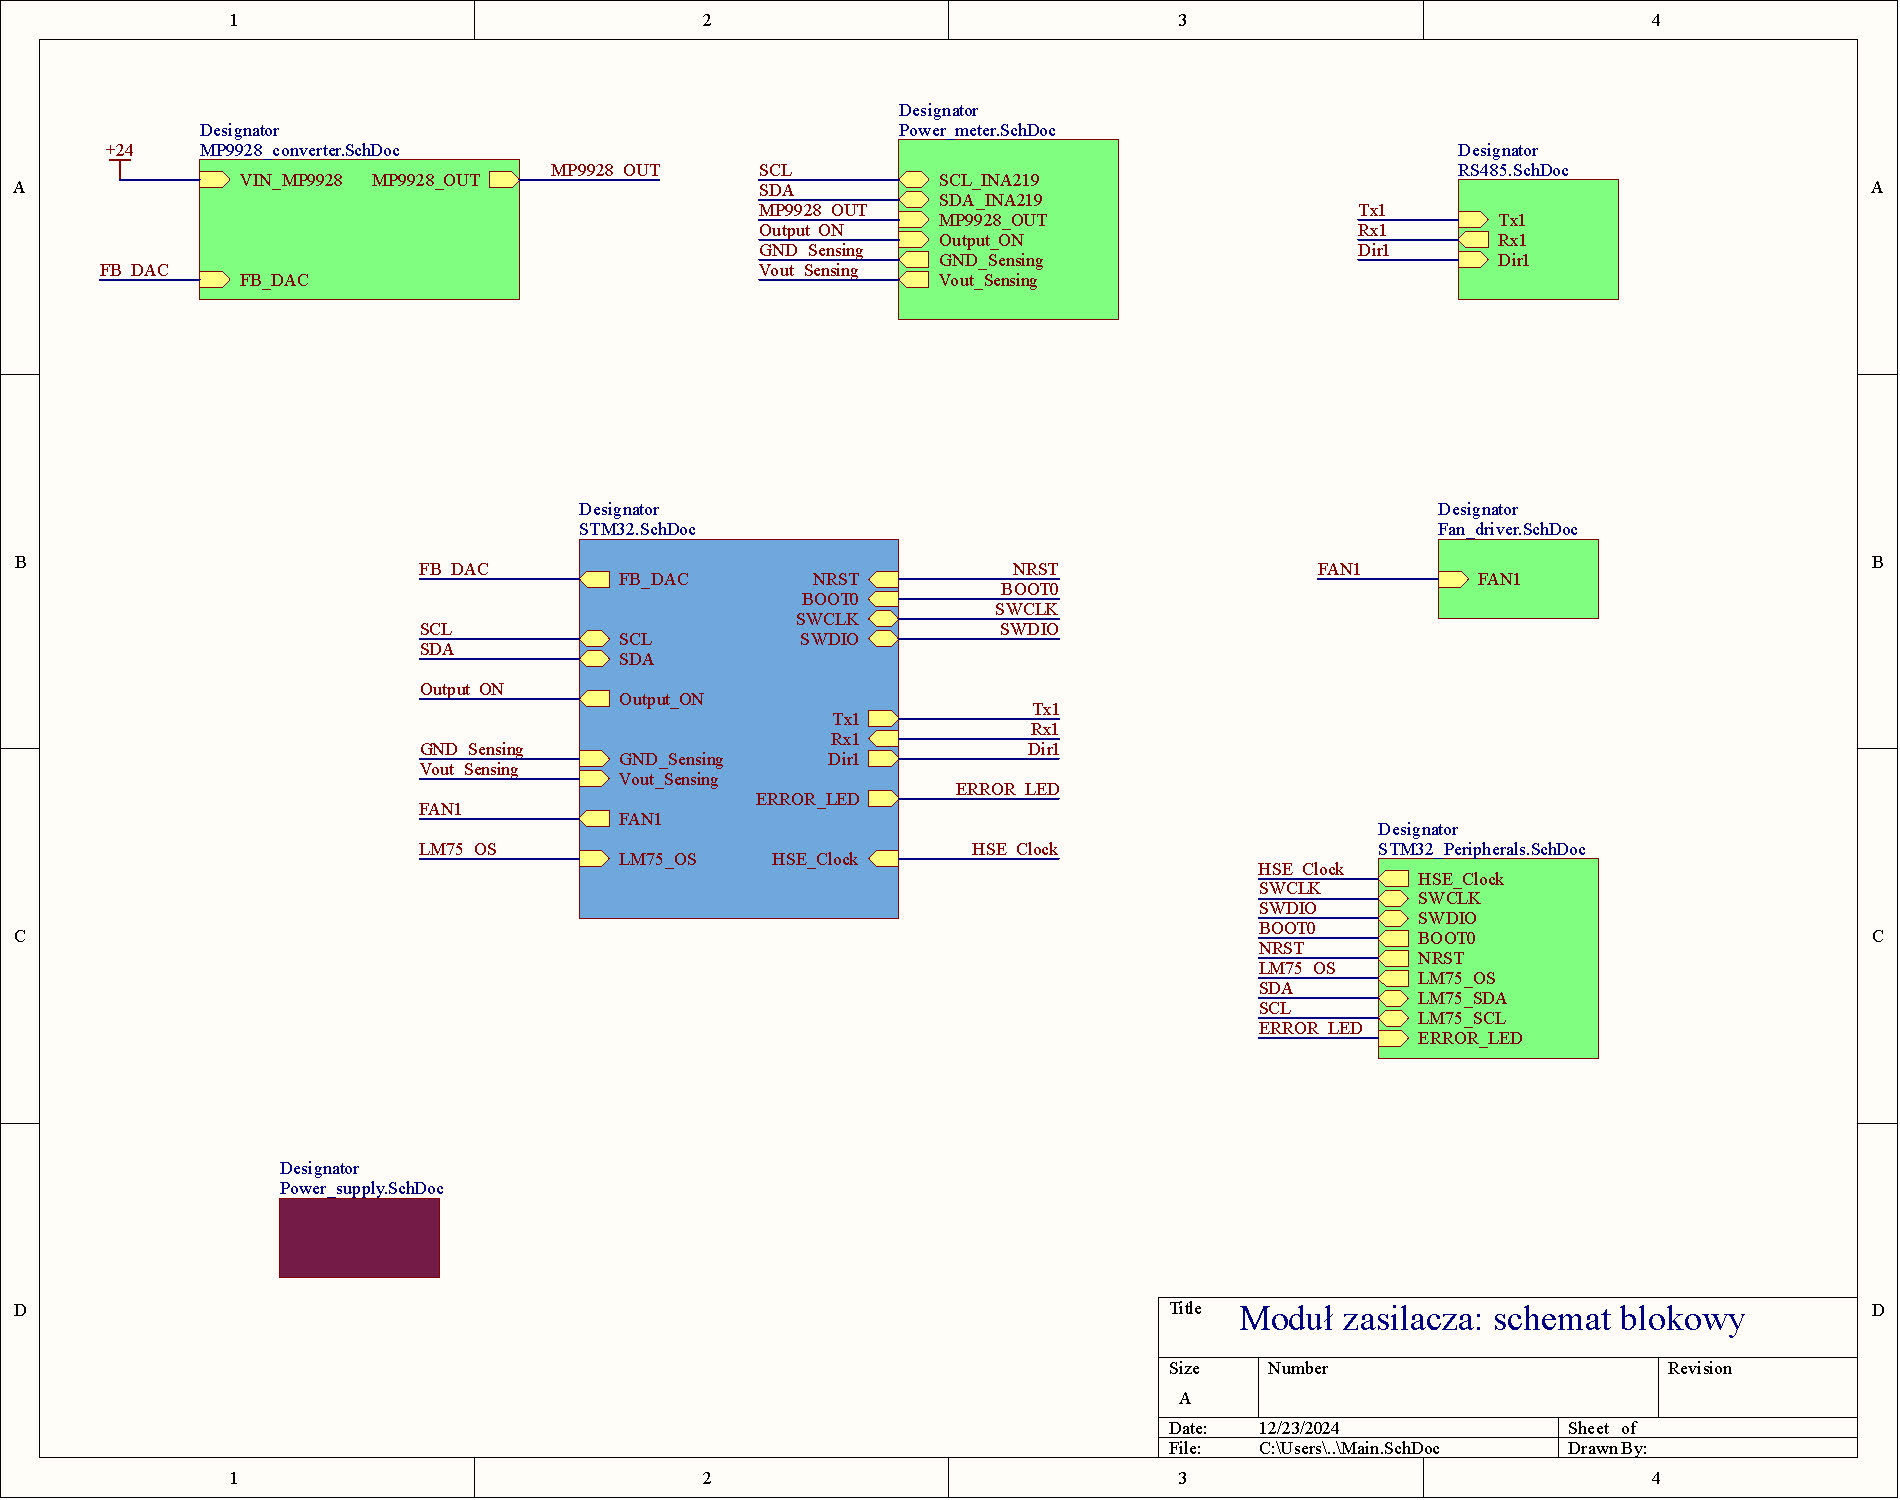
\includegraphics[width = 21cm]{zalaczniki/zasilacz/Zasilacz_regulowany_Strona_01.jpg}
        \caption{Schemat blokowy modułu zasilacza.}
    \end{center}
\end{sidewaysfigure}

\begin{sidewaysfigure}
    \begin{center}
        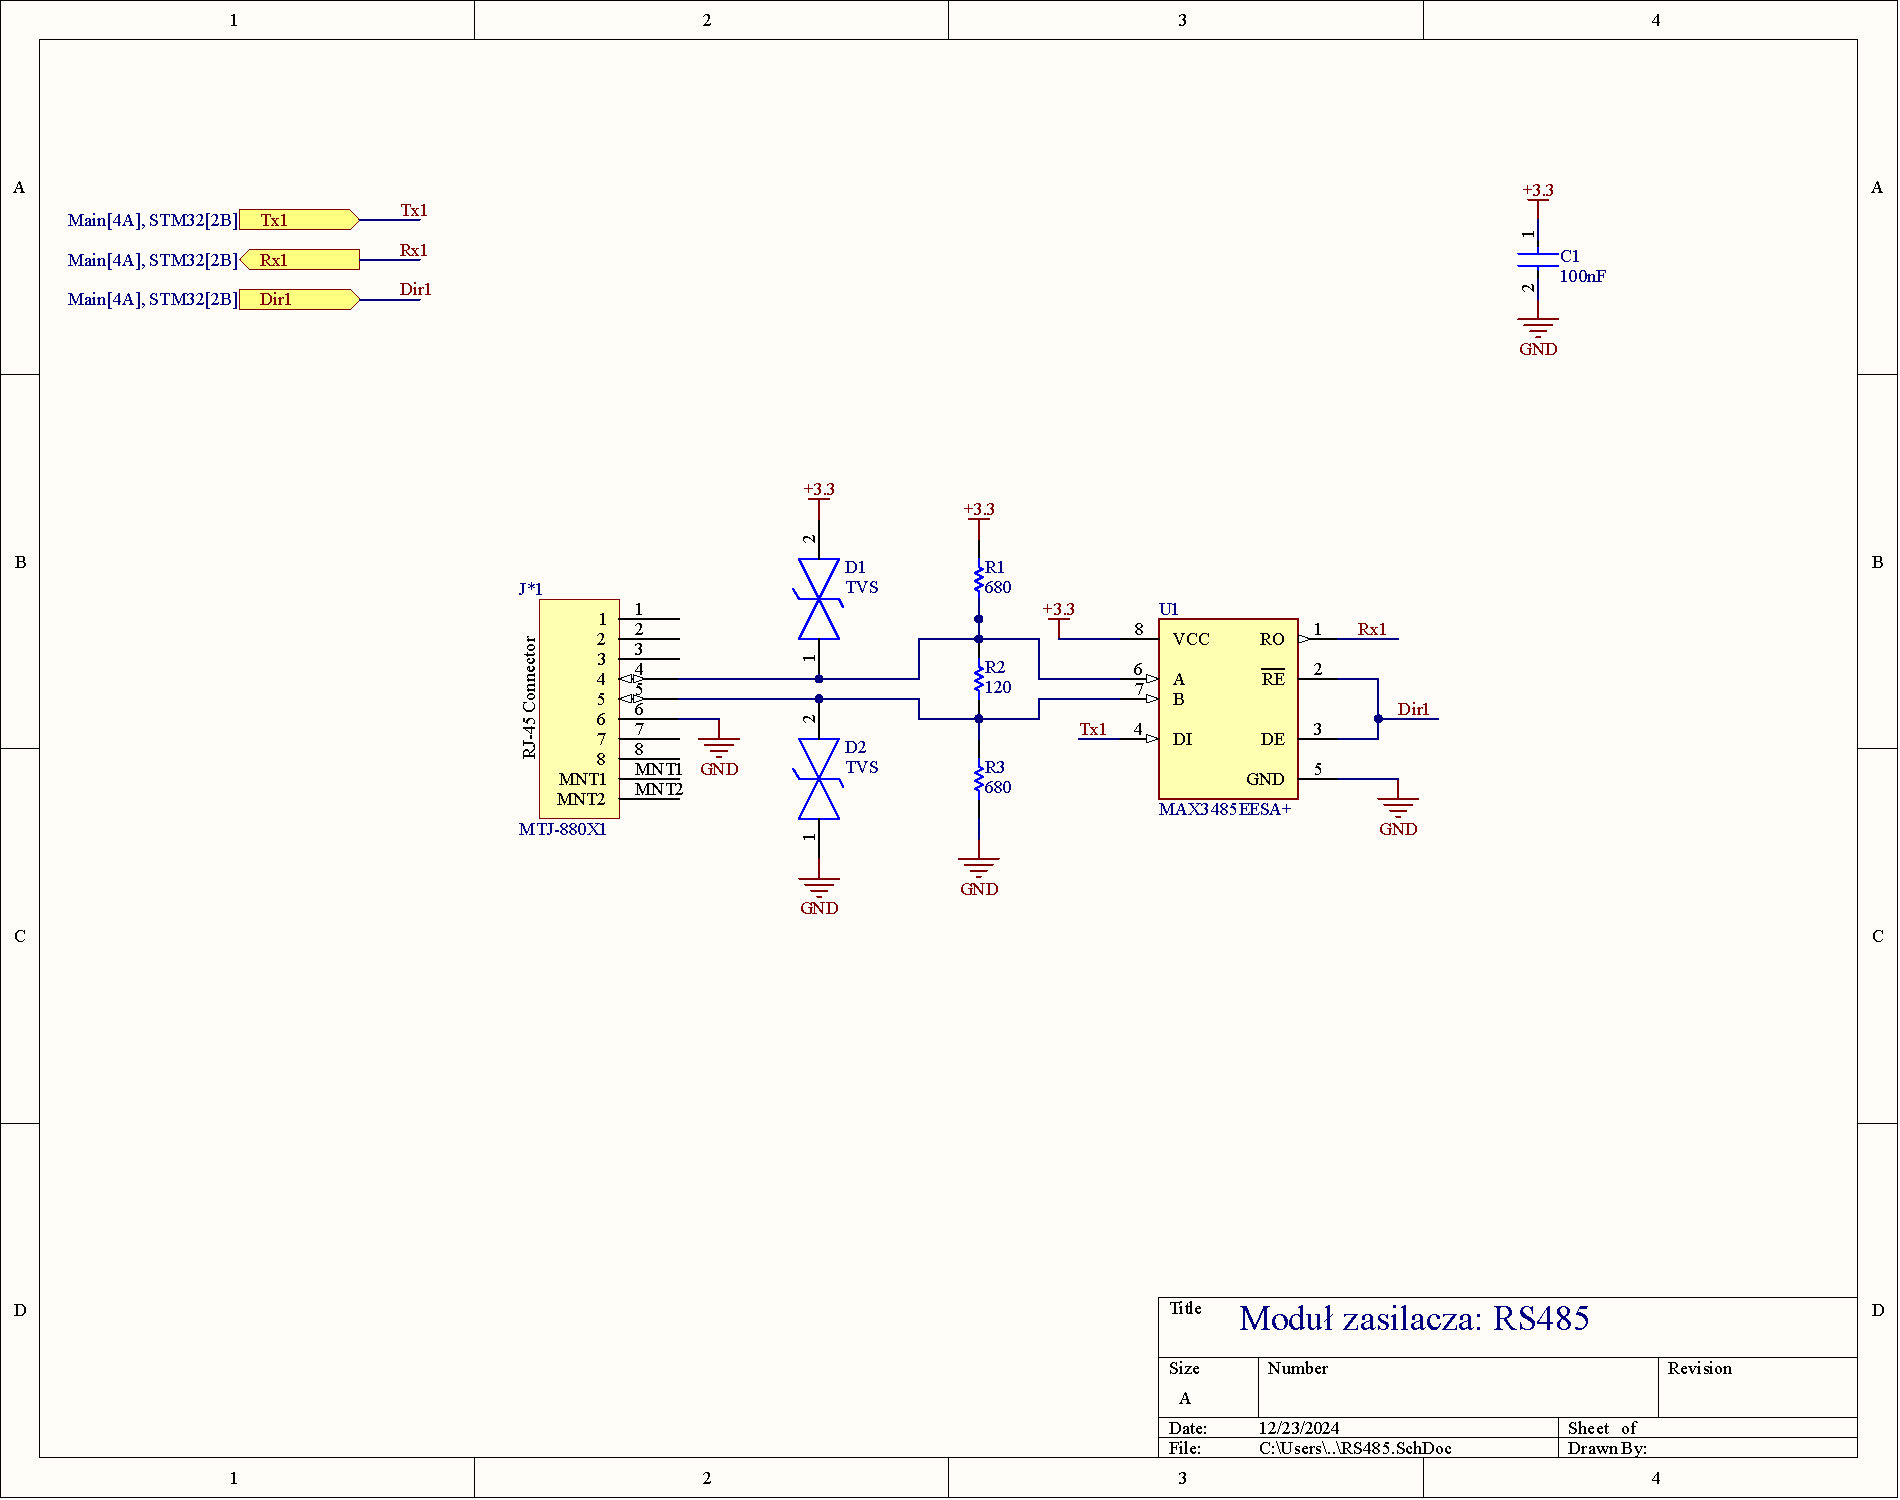
\includegraphics[width = 21cm]{zalaczniki/zasilacz/Zasilacz_regulowany_Strona_02.jpg}
        \caption{Schemat RS485.}
    \end{center}
\end{sidewaysfigure}

\begin{sidewaysfigure}
    \begin{center}
        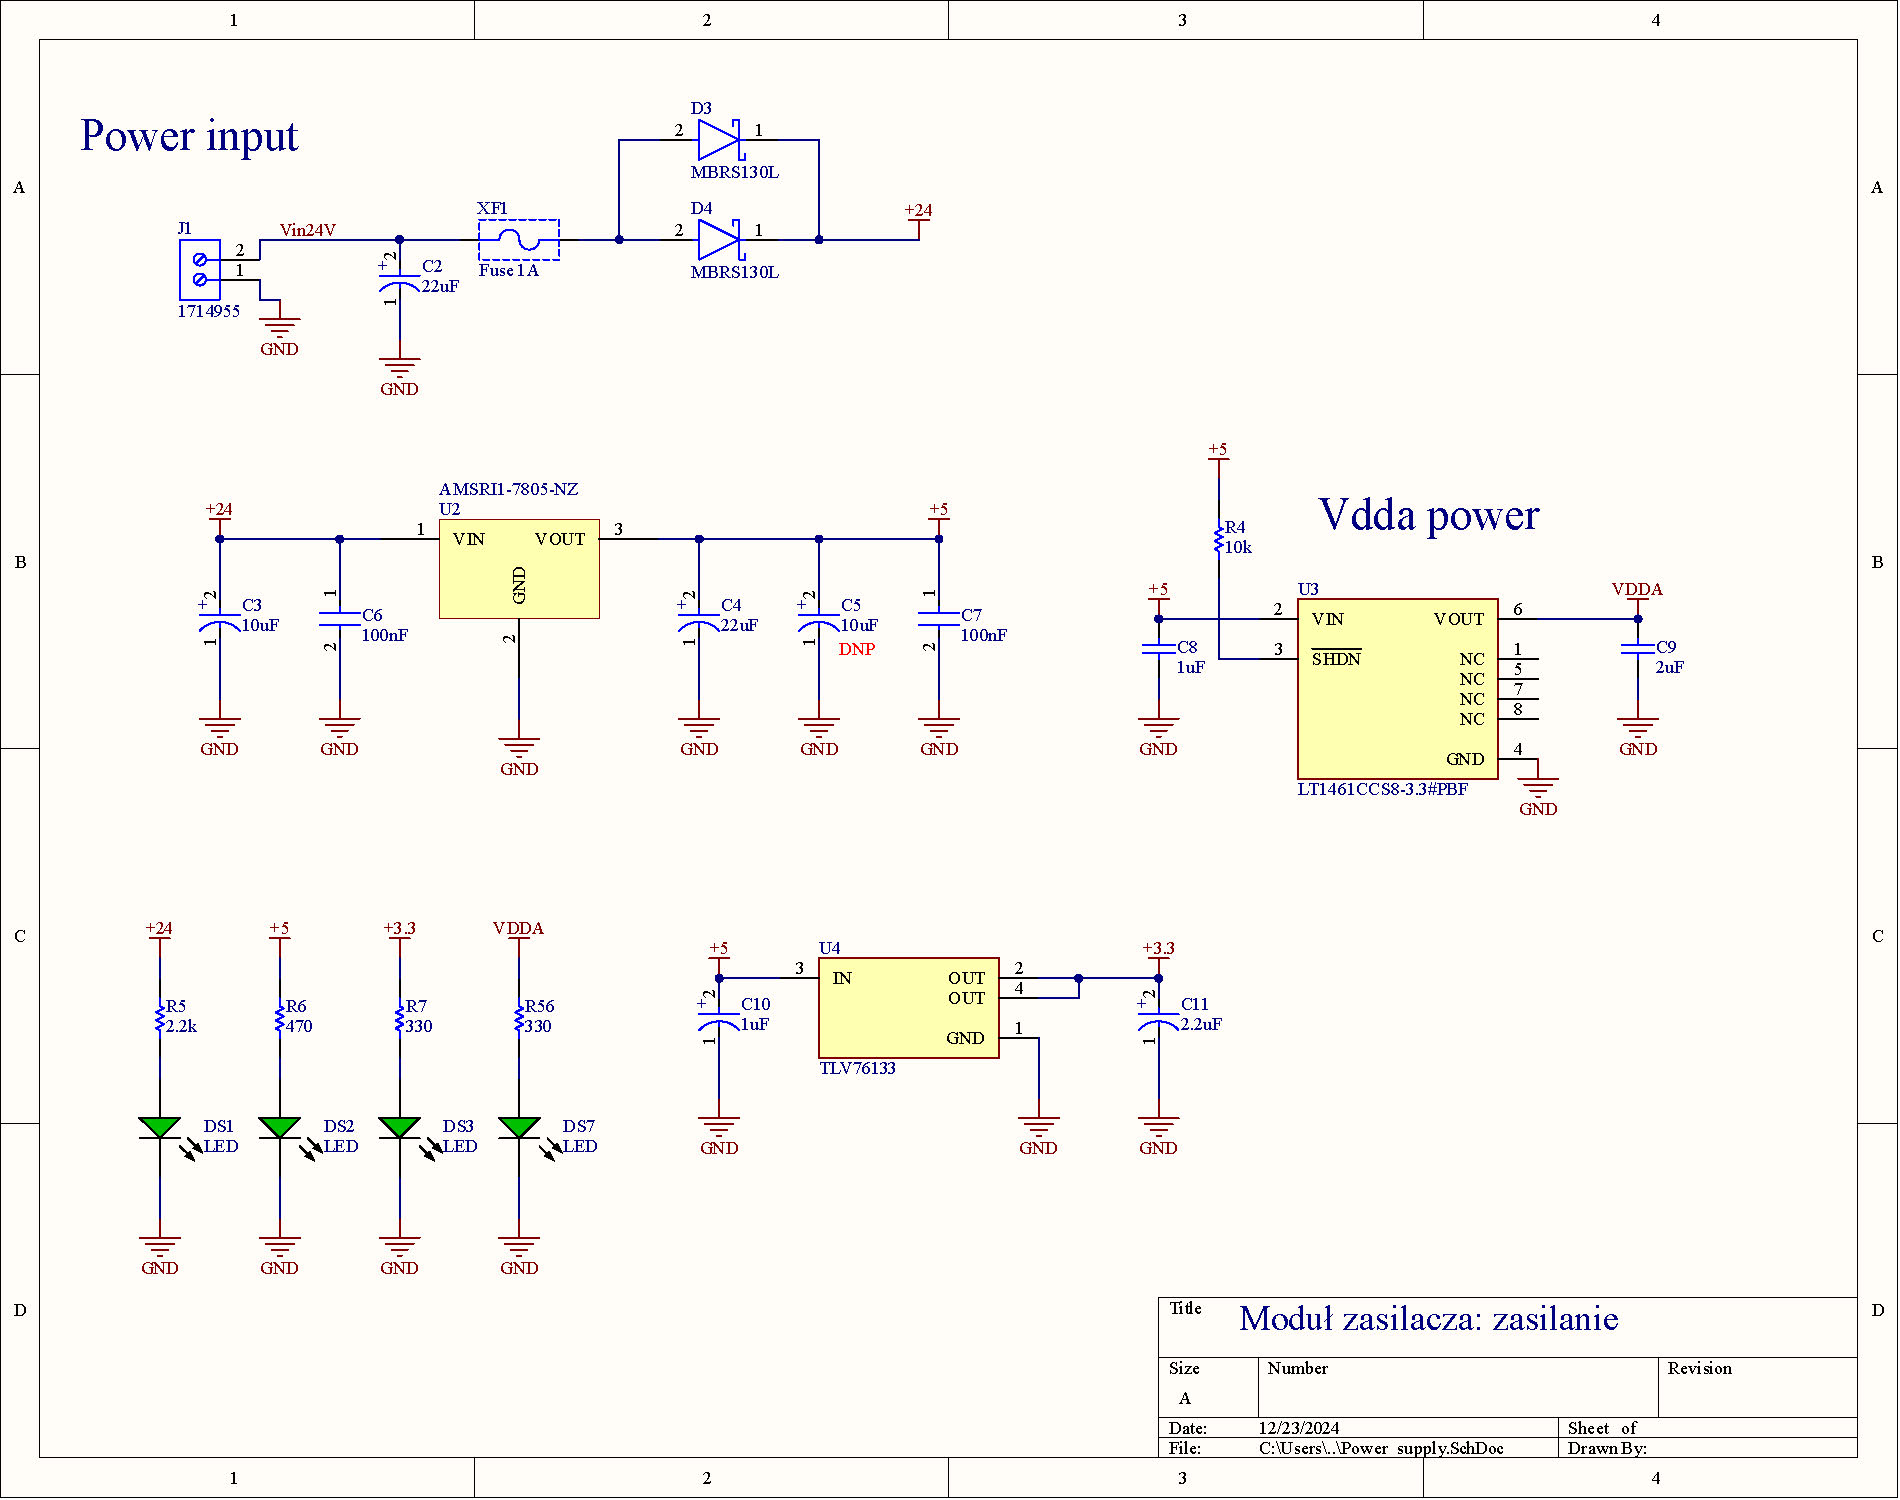
\includegraphics[width = 21cm]{zalaczniki/zasilacz/Zasilacz_regulowany_Strona_03.jpg}
        \caption{Schemat sekcji zasilania.}
    \end{center}
\end{sidewaysfigure}

\begin{sidewaysfigure}
    \begin{center}
        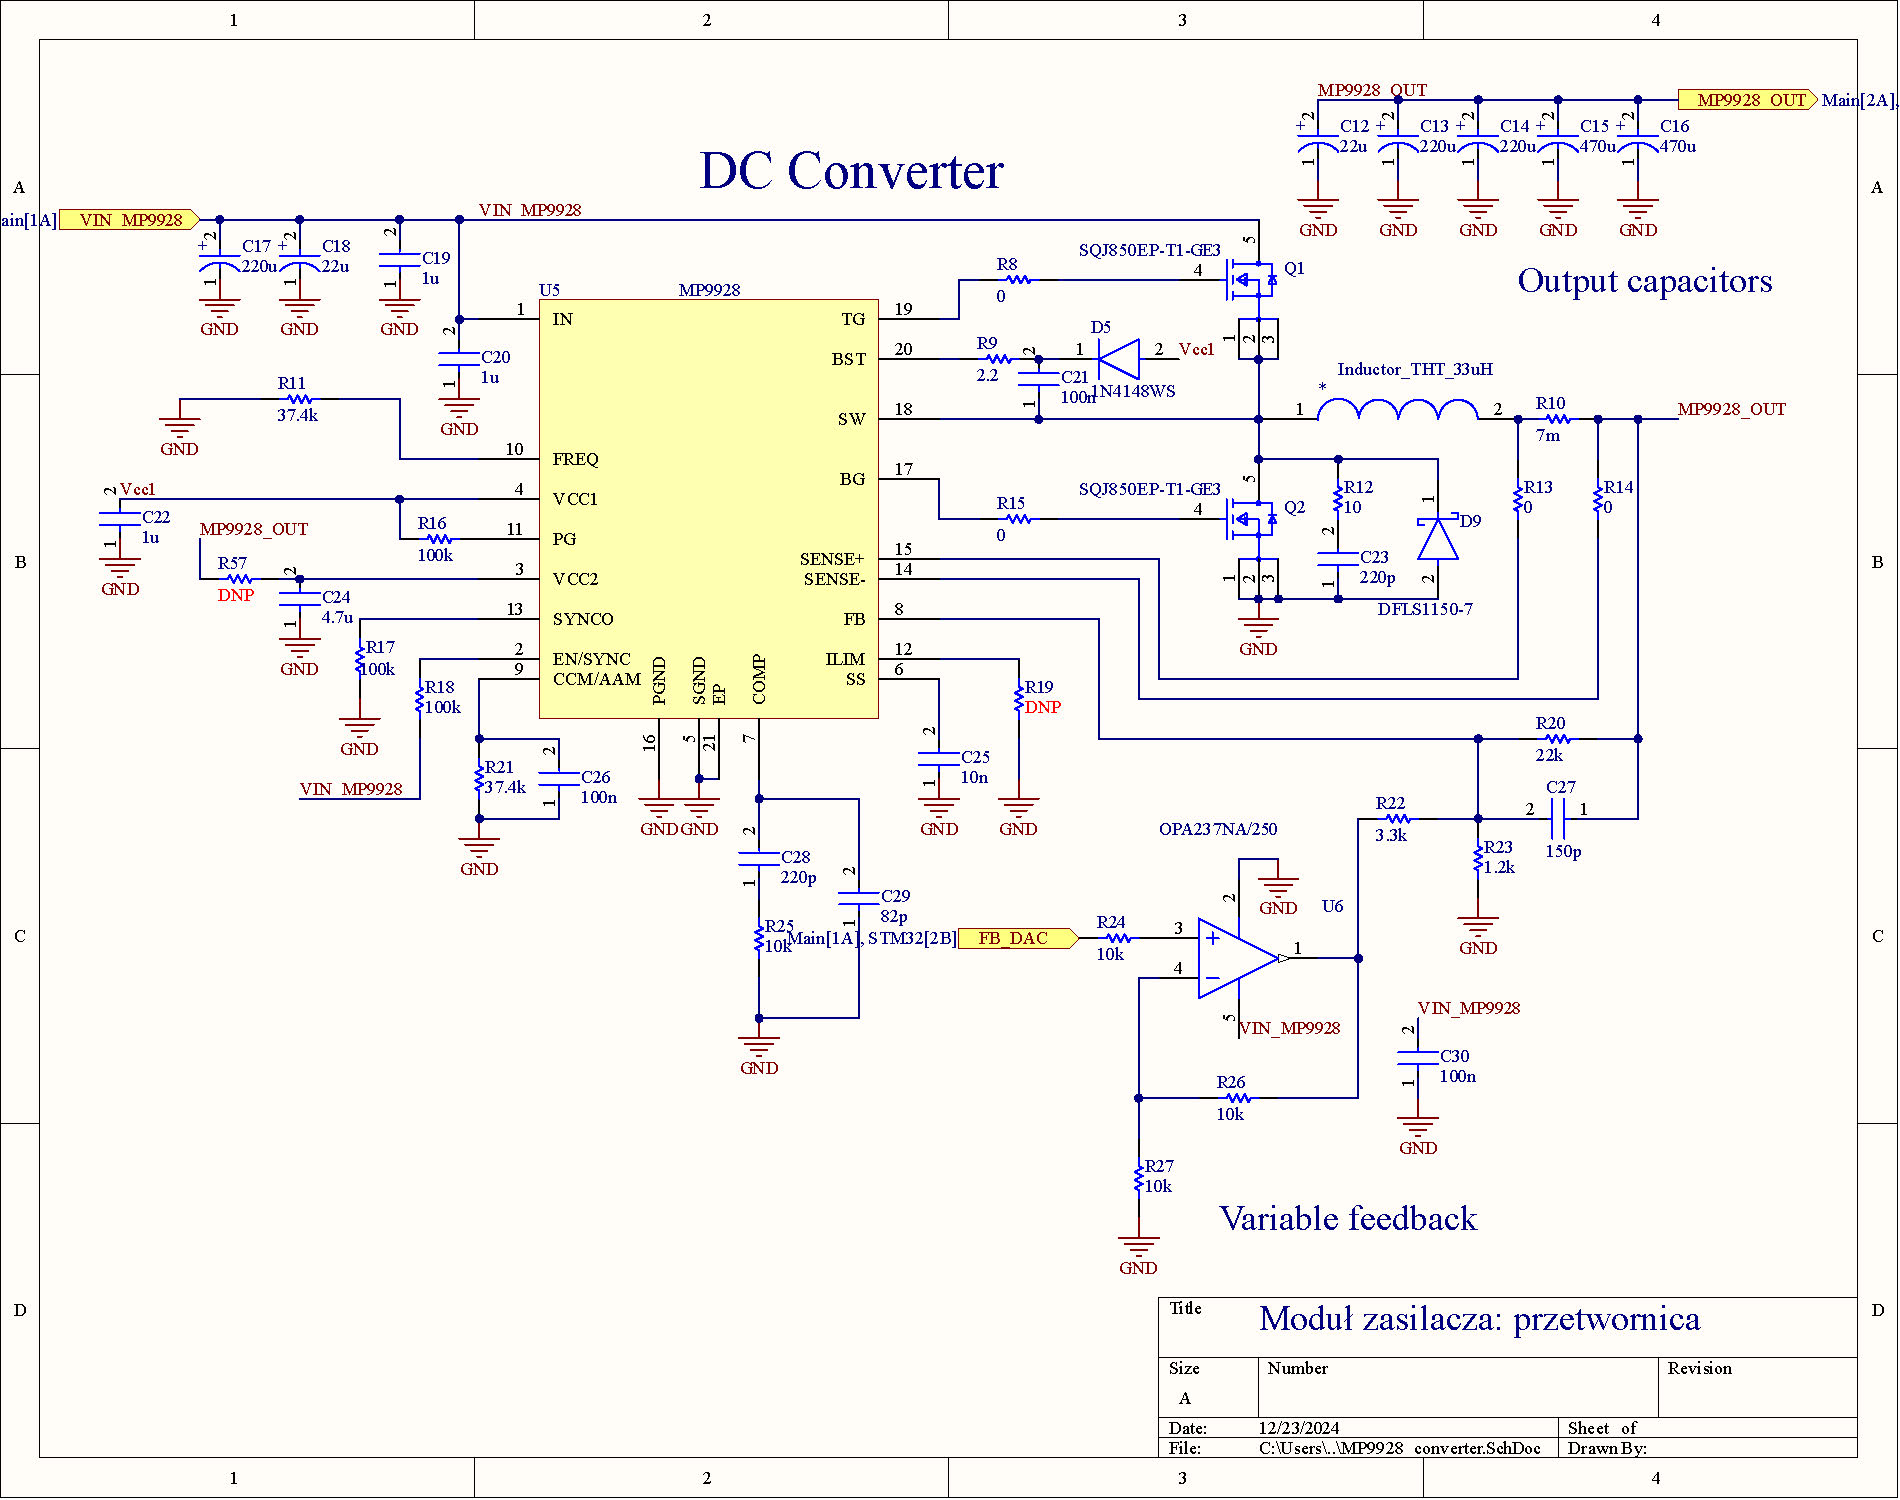
\includegraphics[width = 21cm]{zalaczniki/zasilacz/Zasilacz_regulowany_Strona_04.jpg}
        \caption{Schemat przetwornicy MP9928.}
    \end{center}
\end{sidewaysfigure}

\begin{sidewaysfigure}
    \begin{center}
        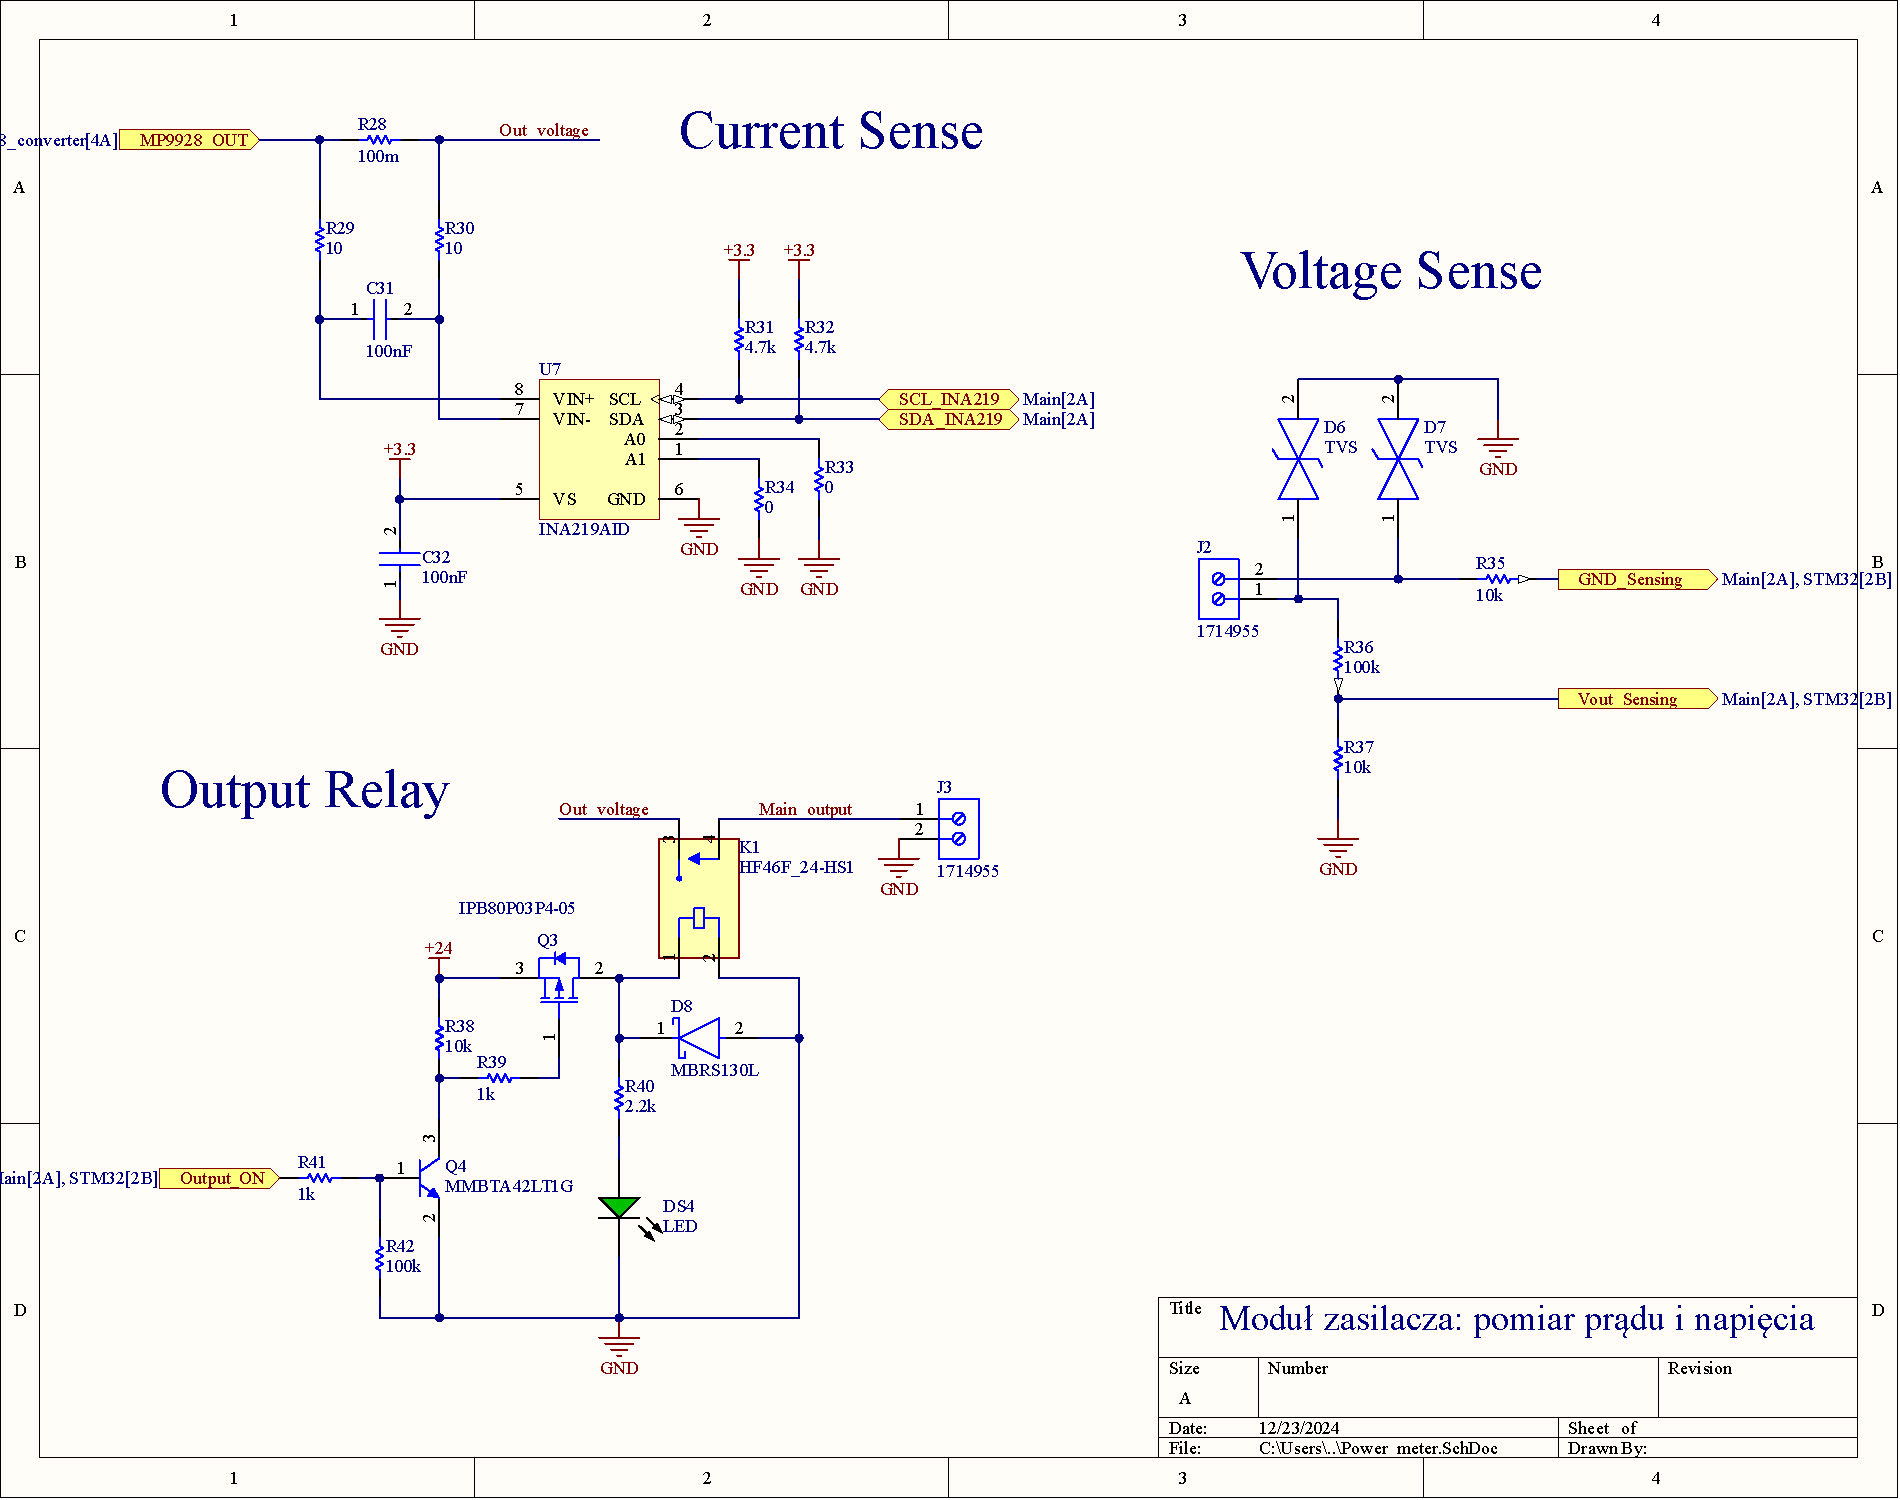
\includegraphics[width = 21cm]{zalaczniki/zasilacz/Zasilacz_regulowany_Strona_05.jpg}
        \caption{Schemat ukladu pomiaru prądu.}
    \end{center}
\end{sidewaysfigure}

\begin{sidewaysfigure}
    \begin{center}
        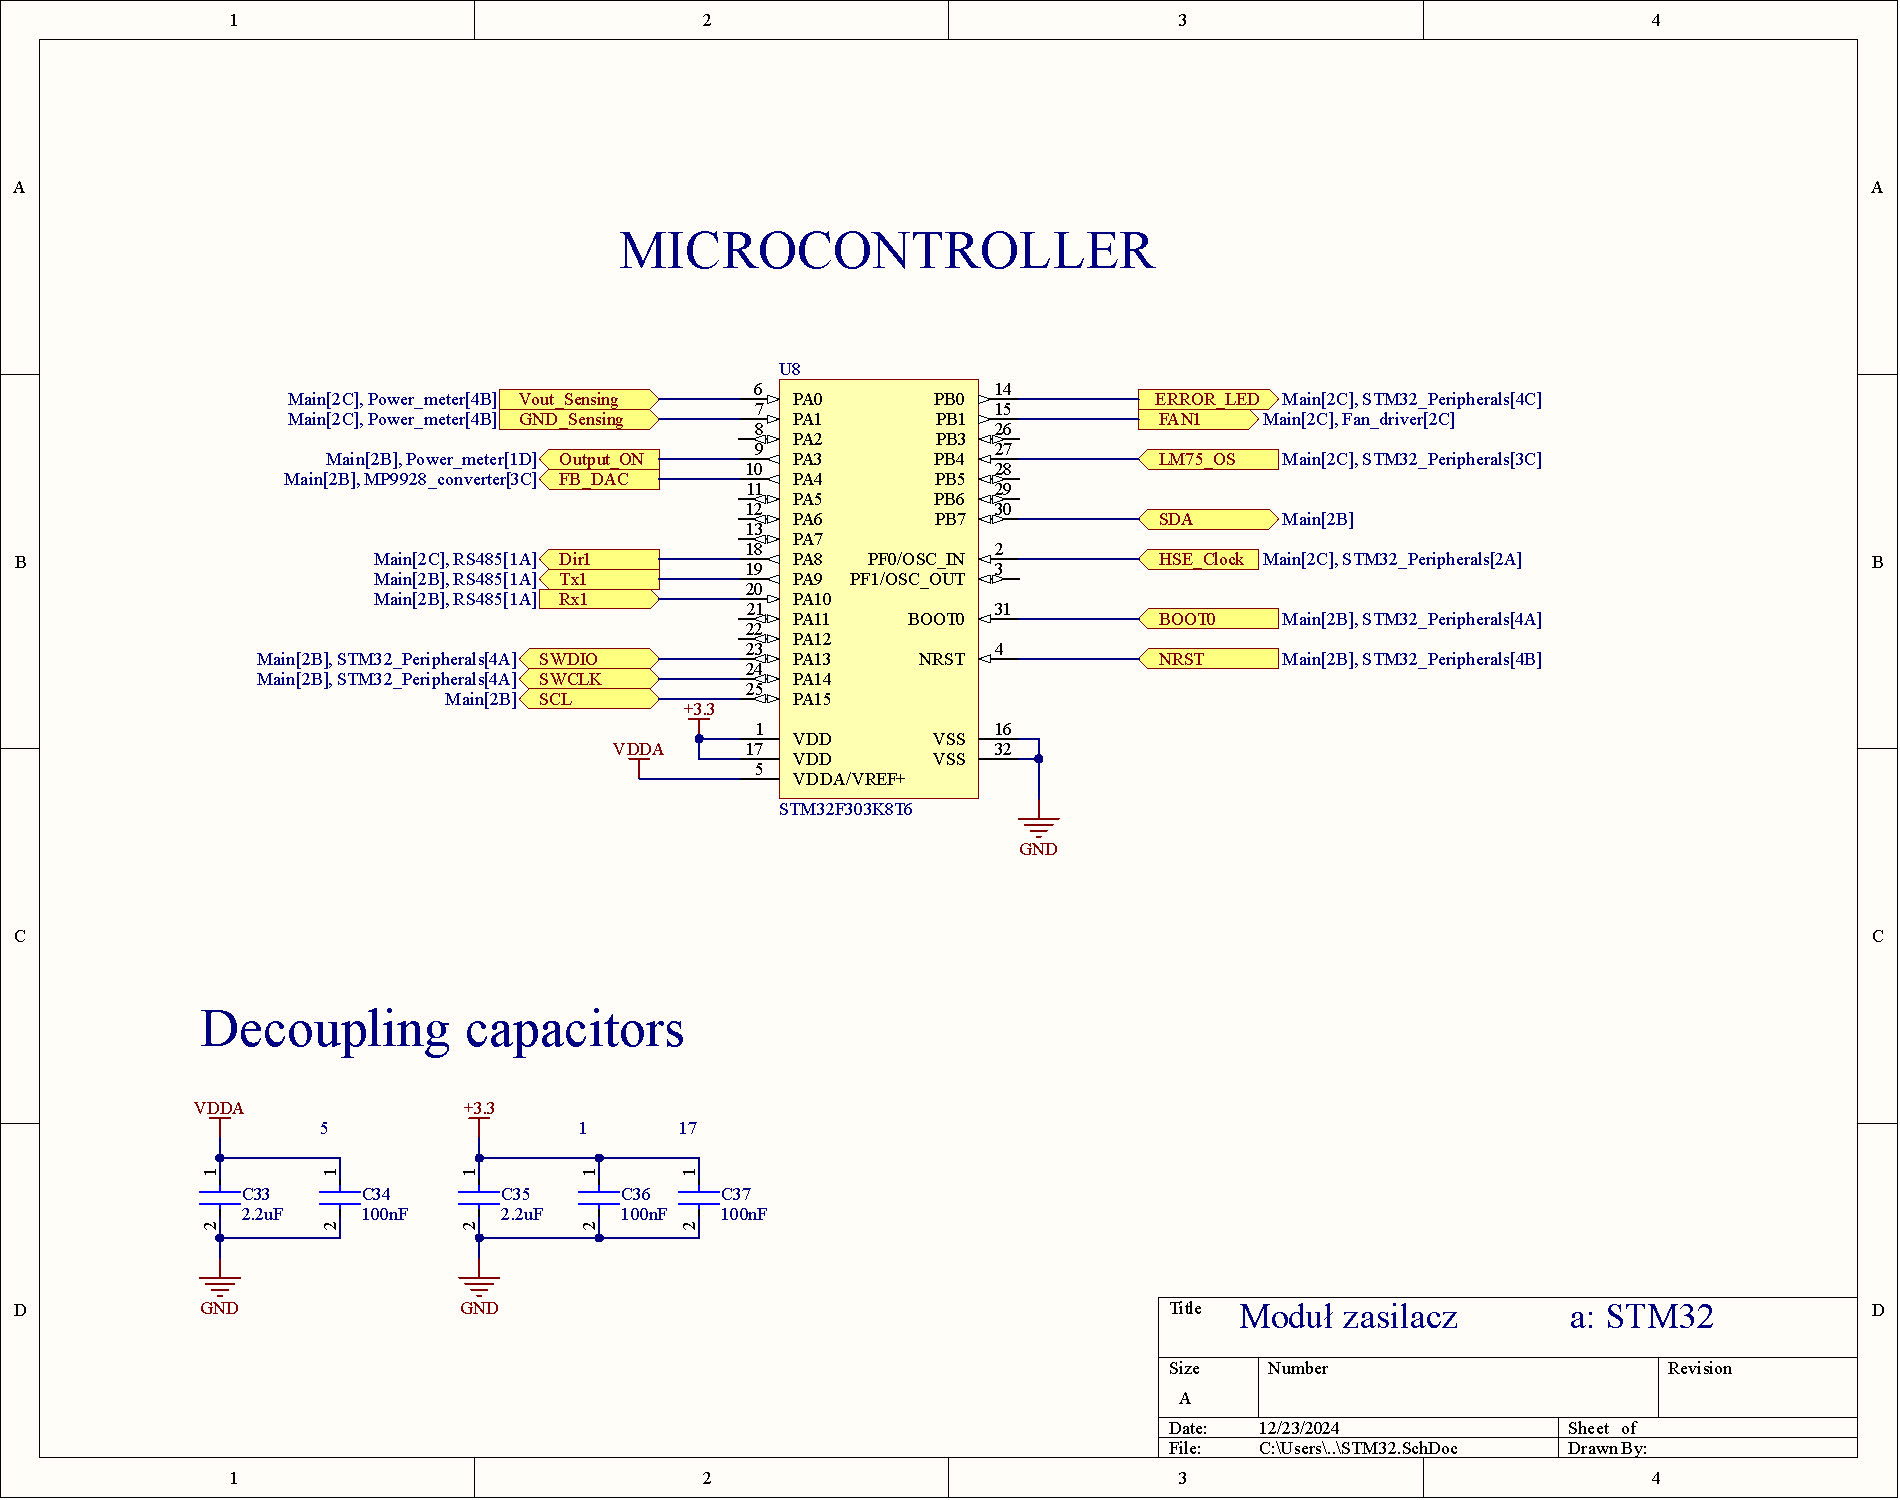
\includegraphics[width = 21cm]{zalaczniki/zasilacz/Zasilacz_regulowany_Strona_06.jpg}
        \caption{Schemat mikrokontrolera STM32.}
    \end{center}
\end{sidewaysfigure}

\begin{sidewaysfigure}
    \begin{center}
        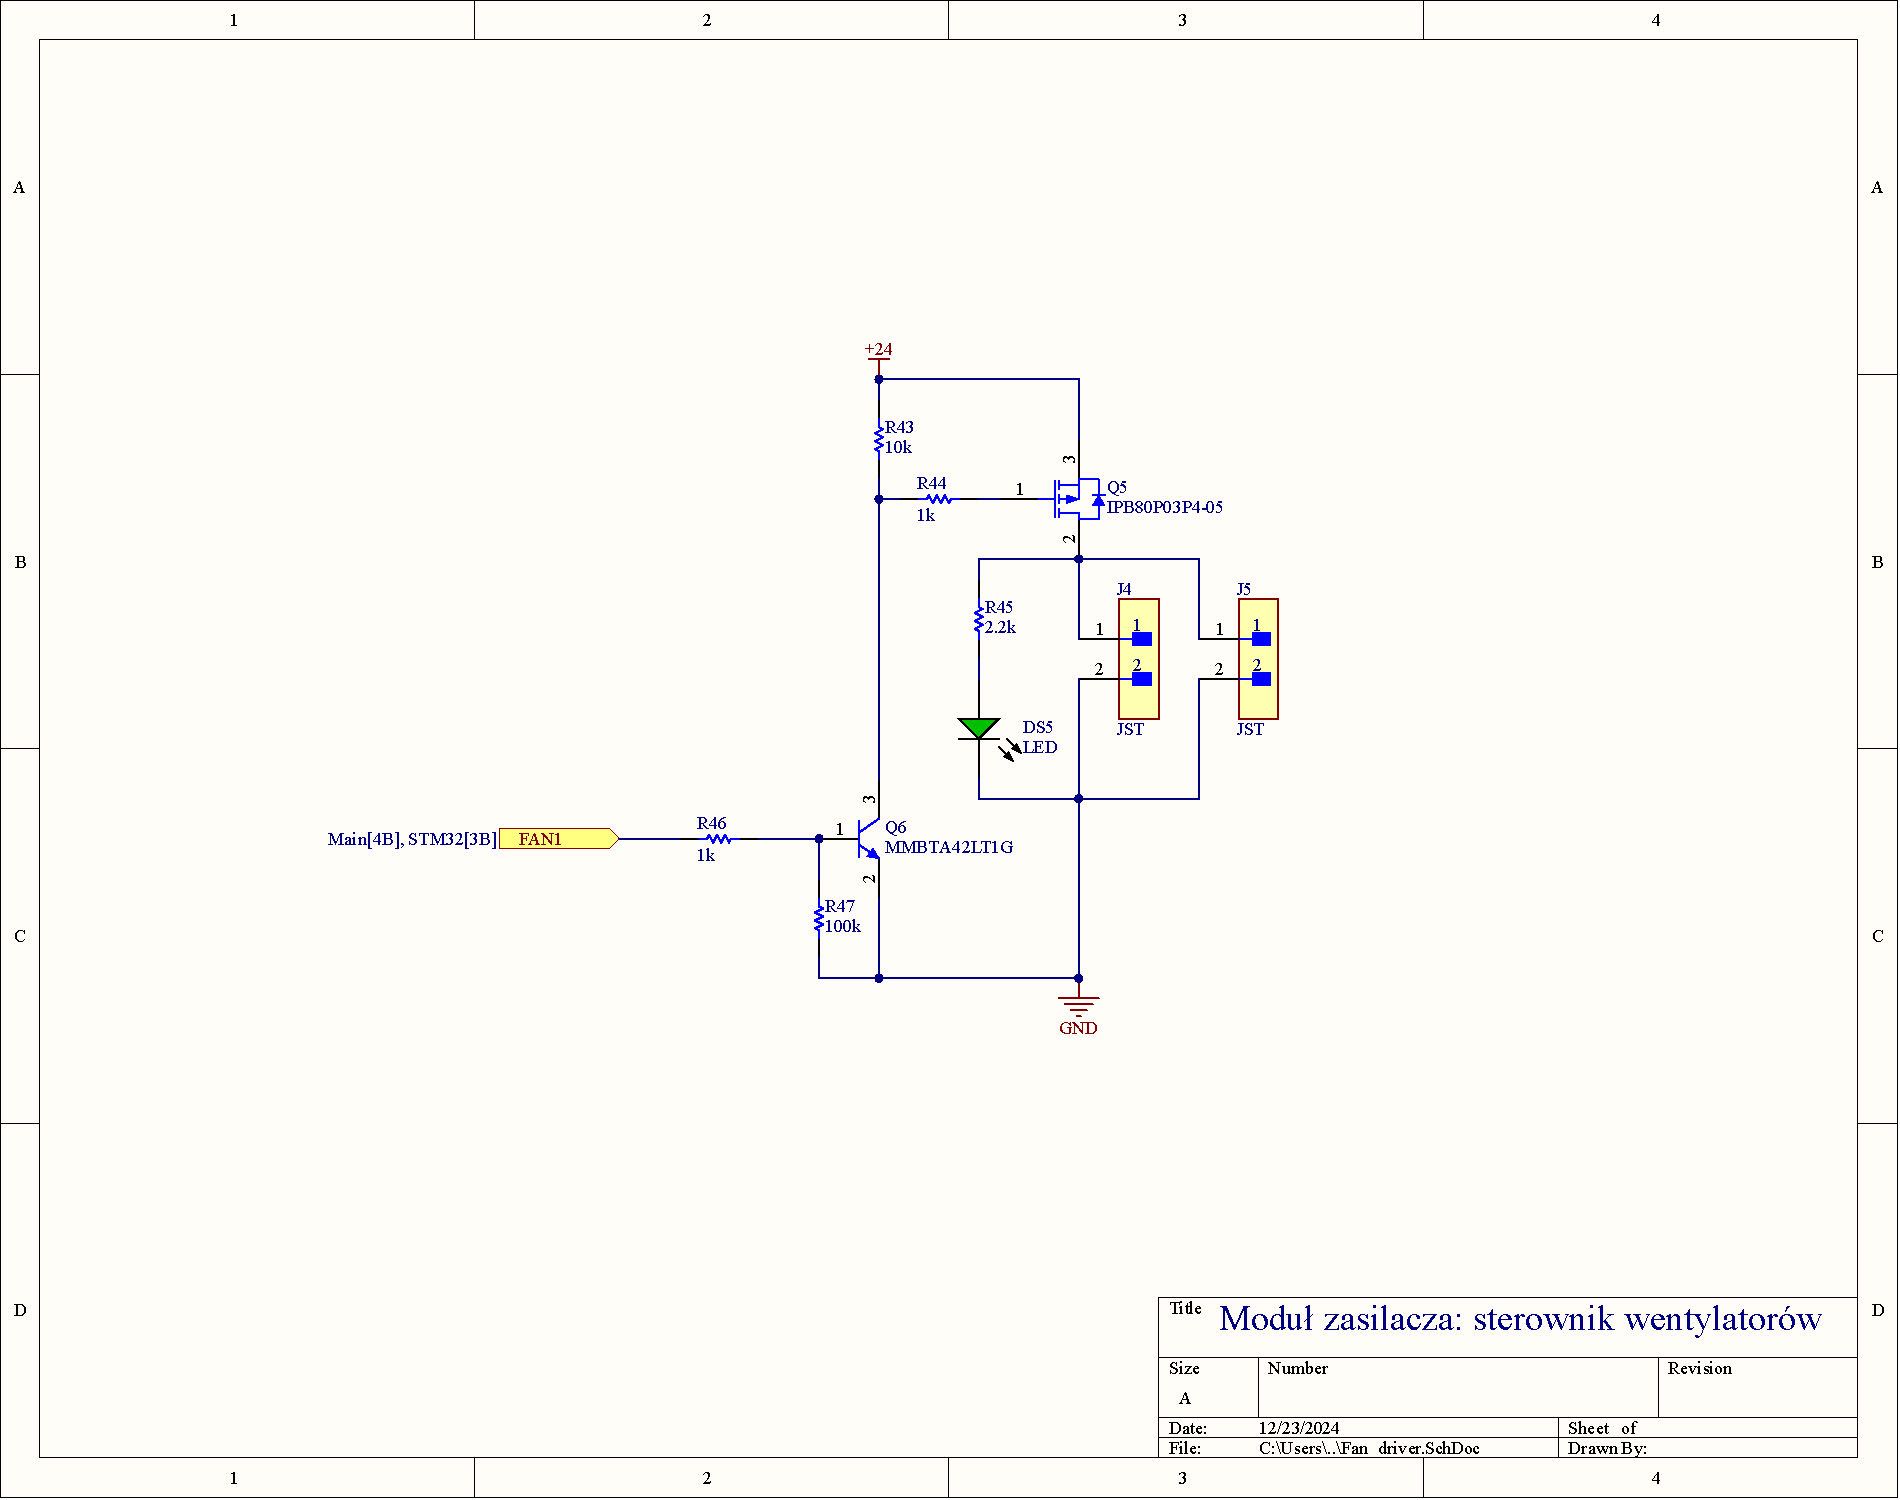
\includegraphics[width = 21cm]{zalaczniki/zasilacz/Zasilacz_regulowany_Strona_07.jpg}
        \caption{Schemat sterownika wentylatorów.}
    \end{center}
\end{sidewaysfigure}

\begin{sidewaysfigure}
    \begin{center}
        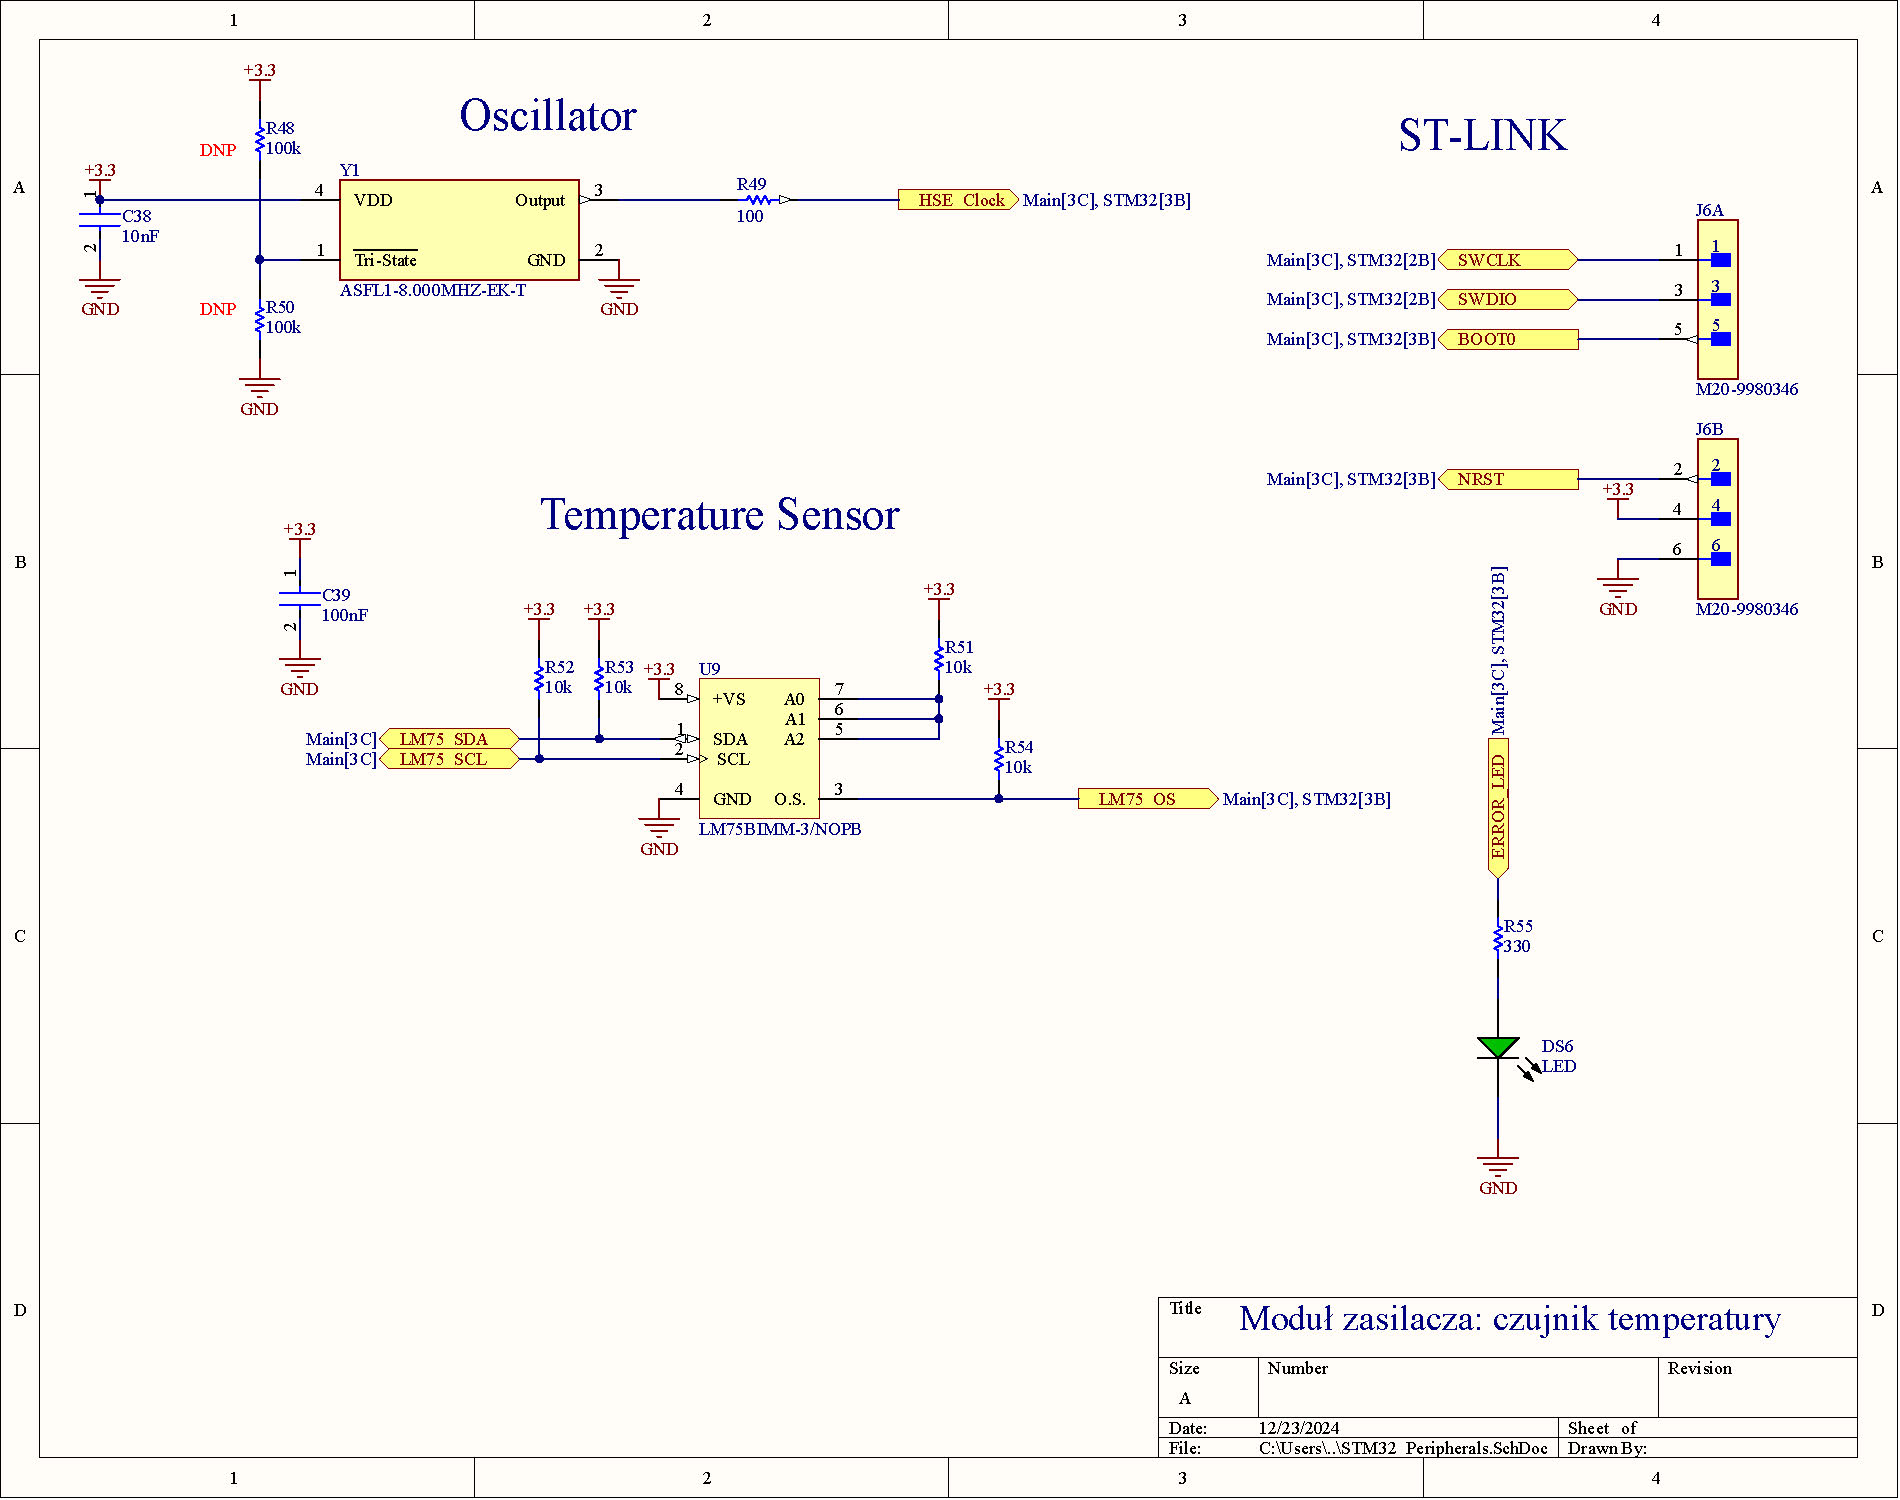
\includegraphics[width = 21cm]{zalaczniki/zasilacz/Zasilacz_regulowany_Strona_08.jpg}
        \caption{Schemat układów peryferyjnych.}
    \end{center}
\end{sidewaysfigure}

\begin{figure}
    \begin{center}
        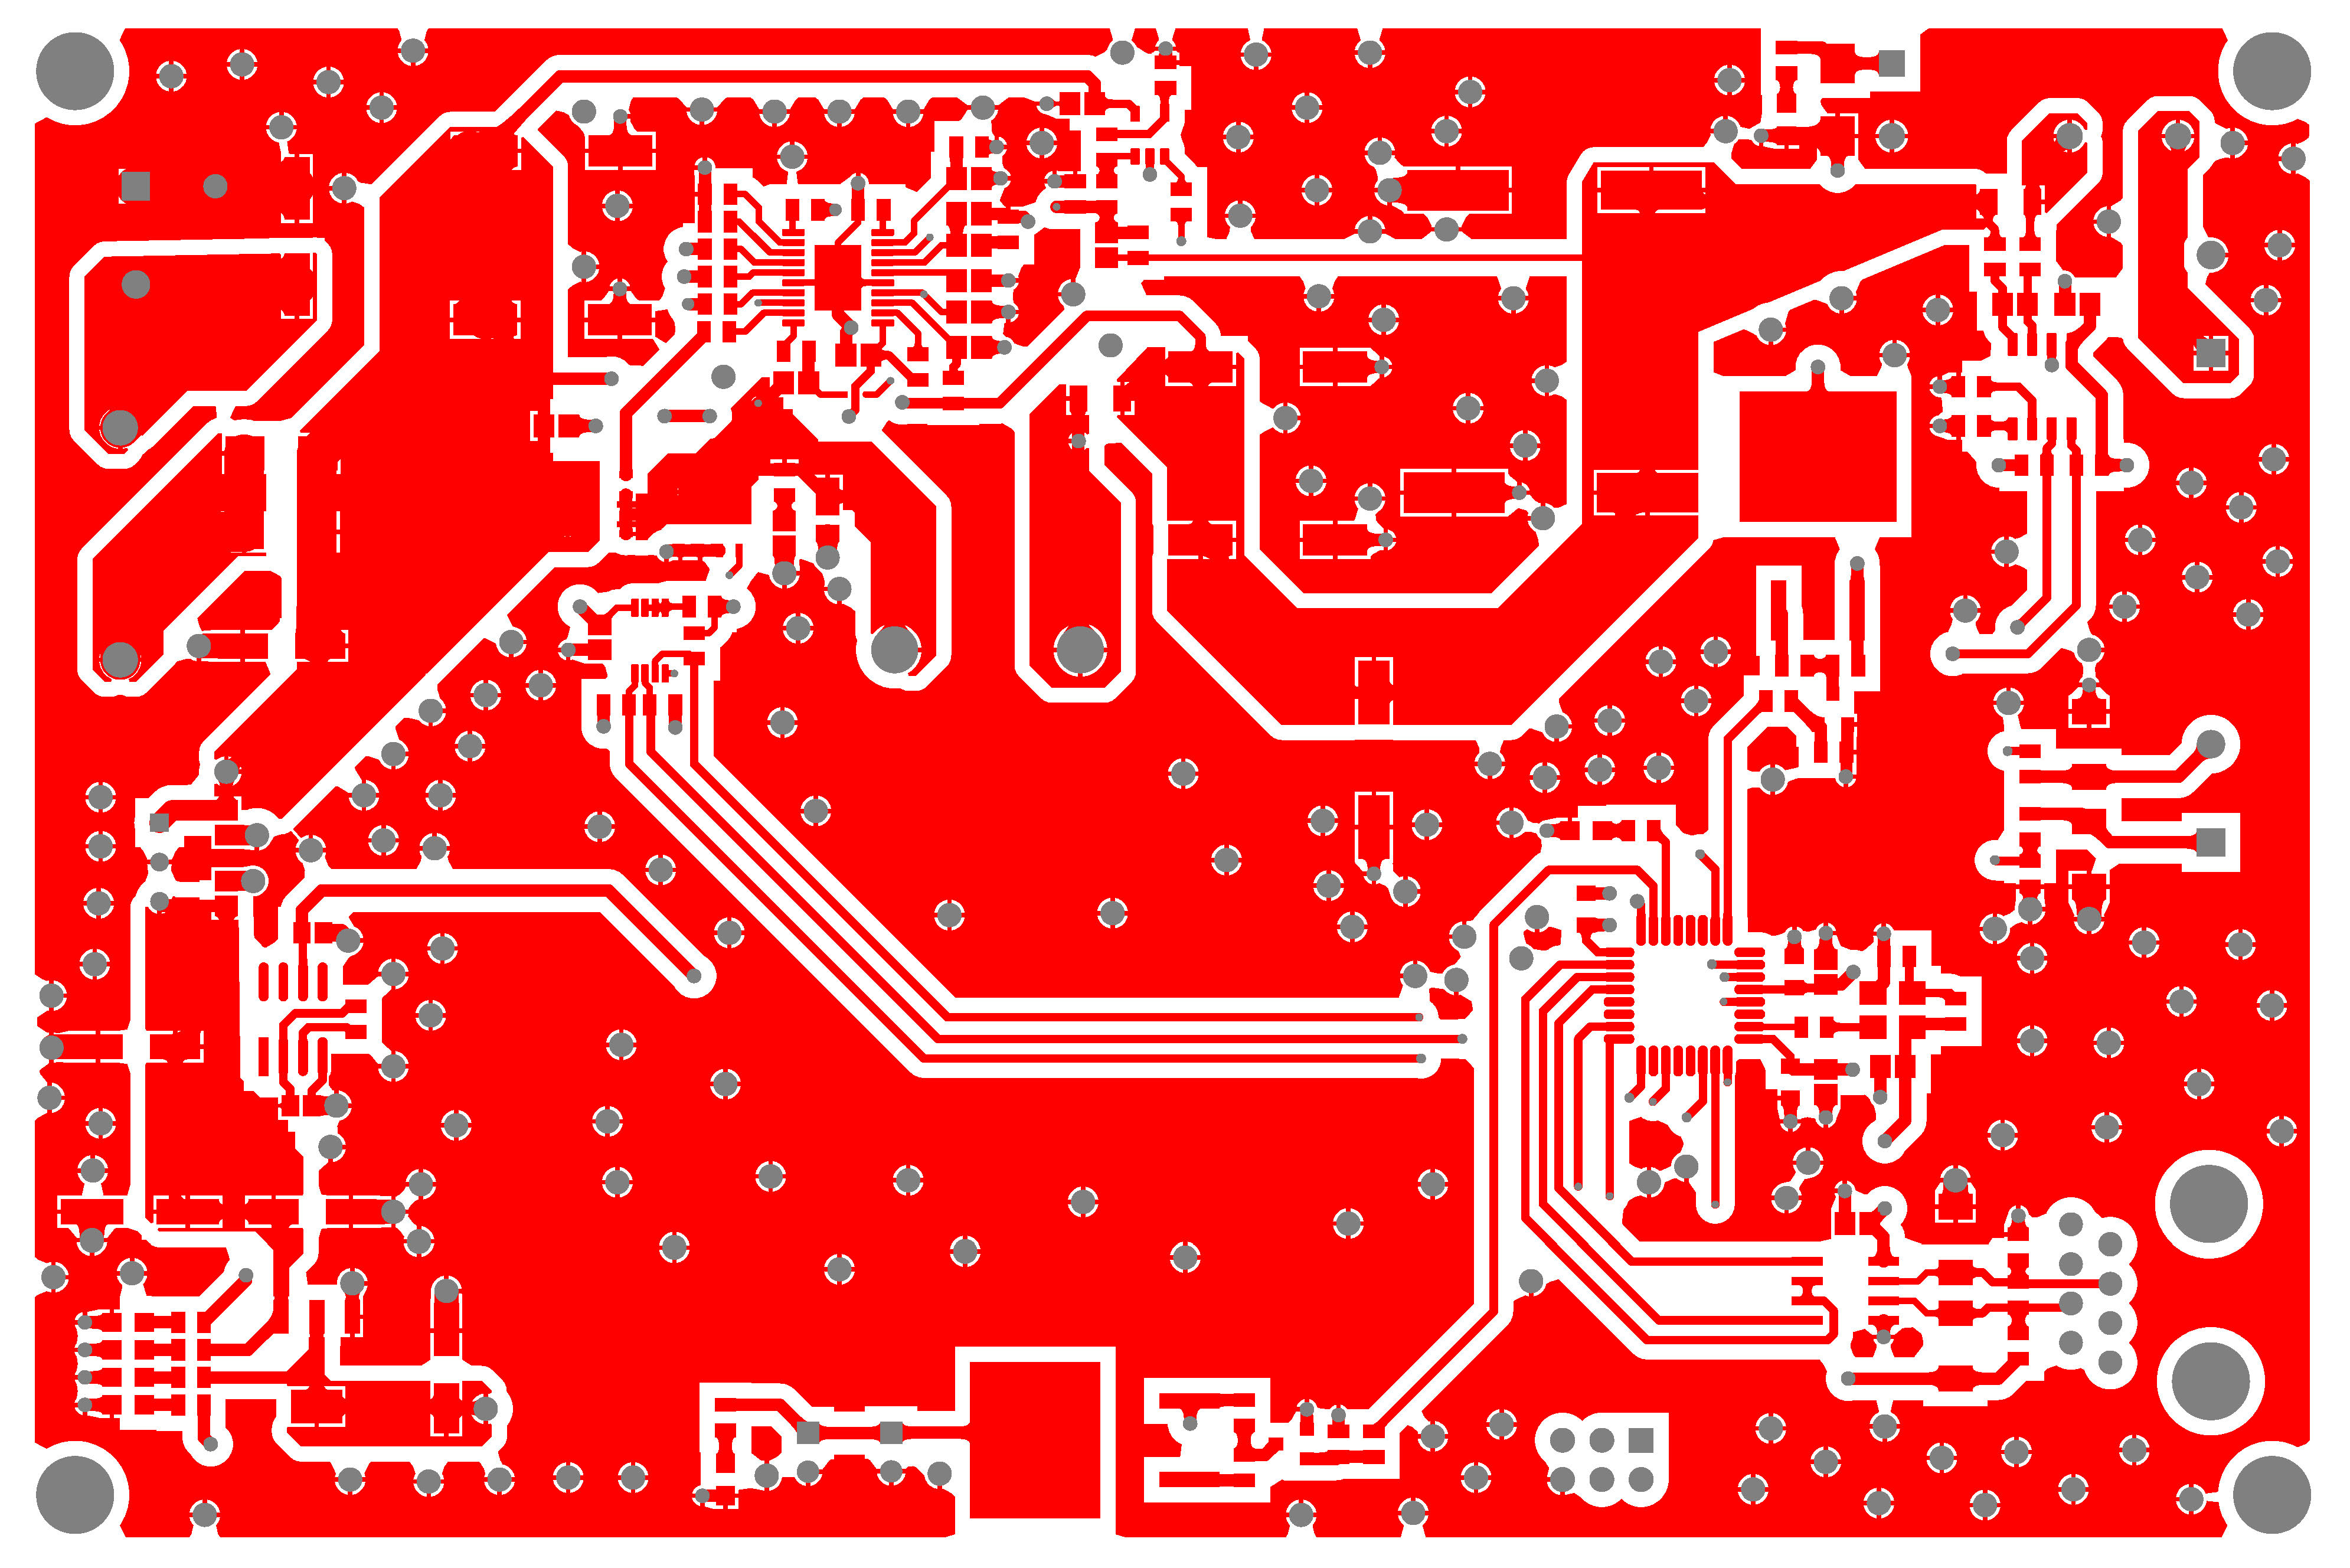
\includegraphics[width = 15cm]{zalaczniki/zasilacz/Zasilacz_regulowany_Strona_09.jpg}
        \caption{Warstwa górna PCB.}
    \end{center}
\end{figure}

\begin{figure}
    \begin{center}
        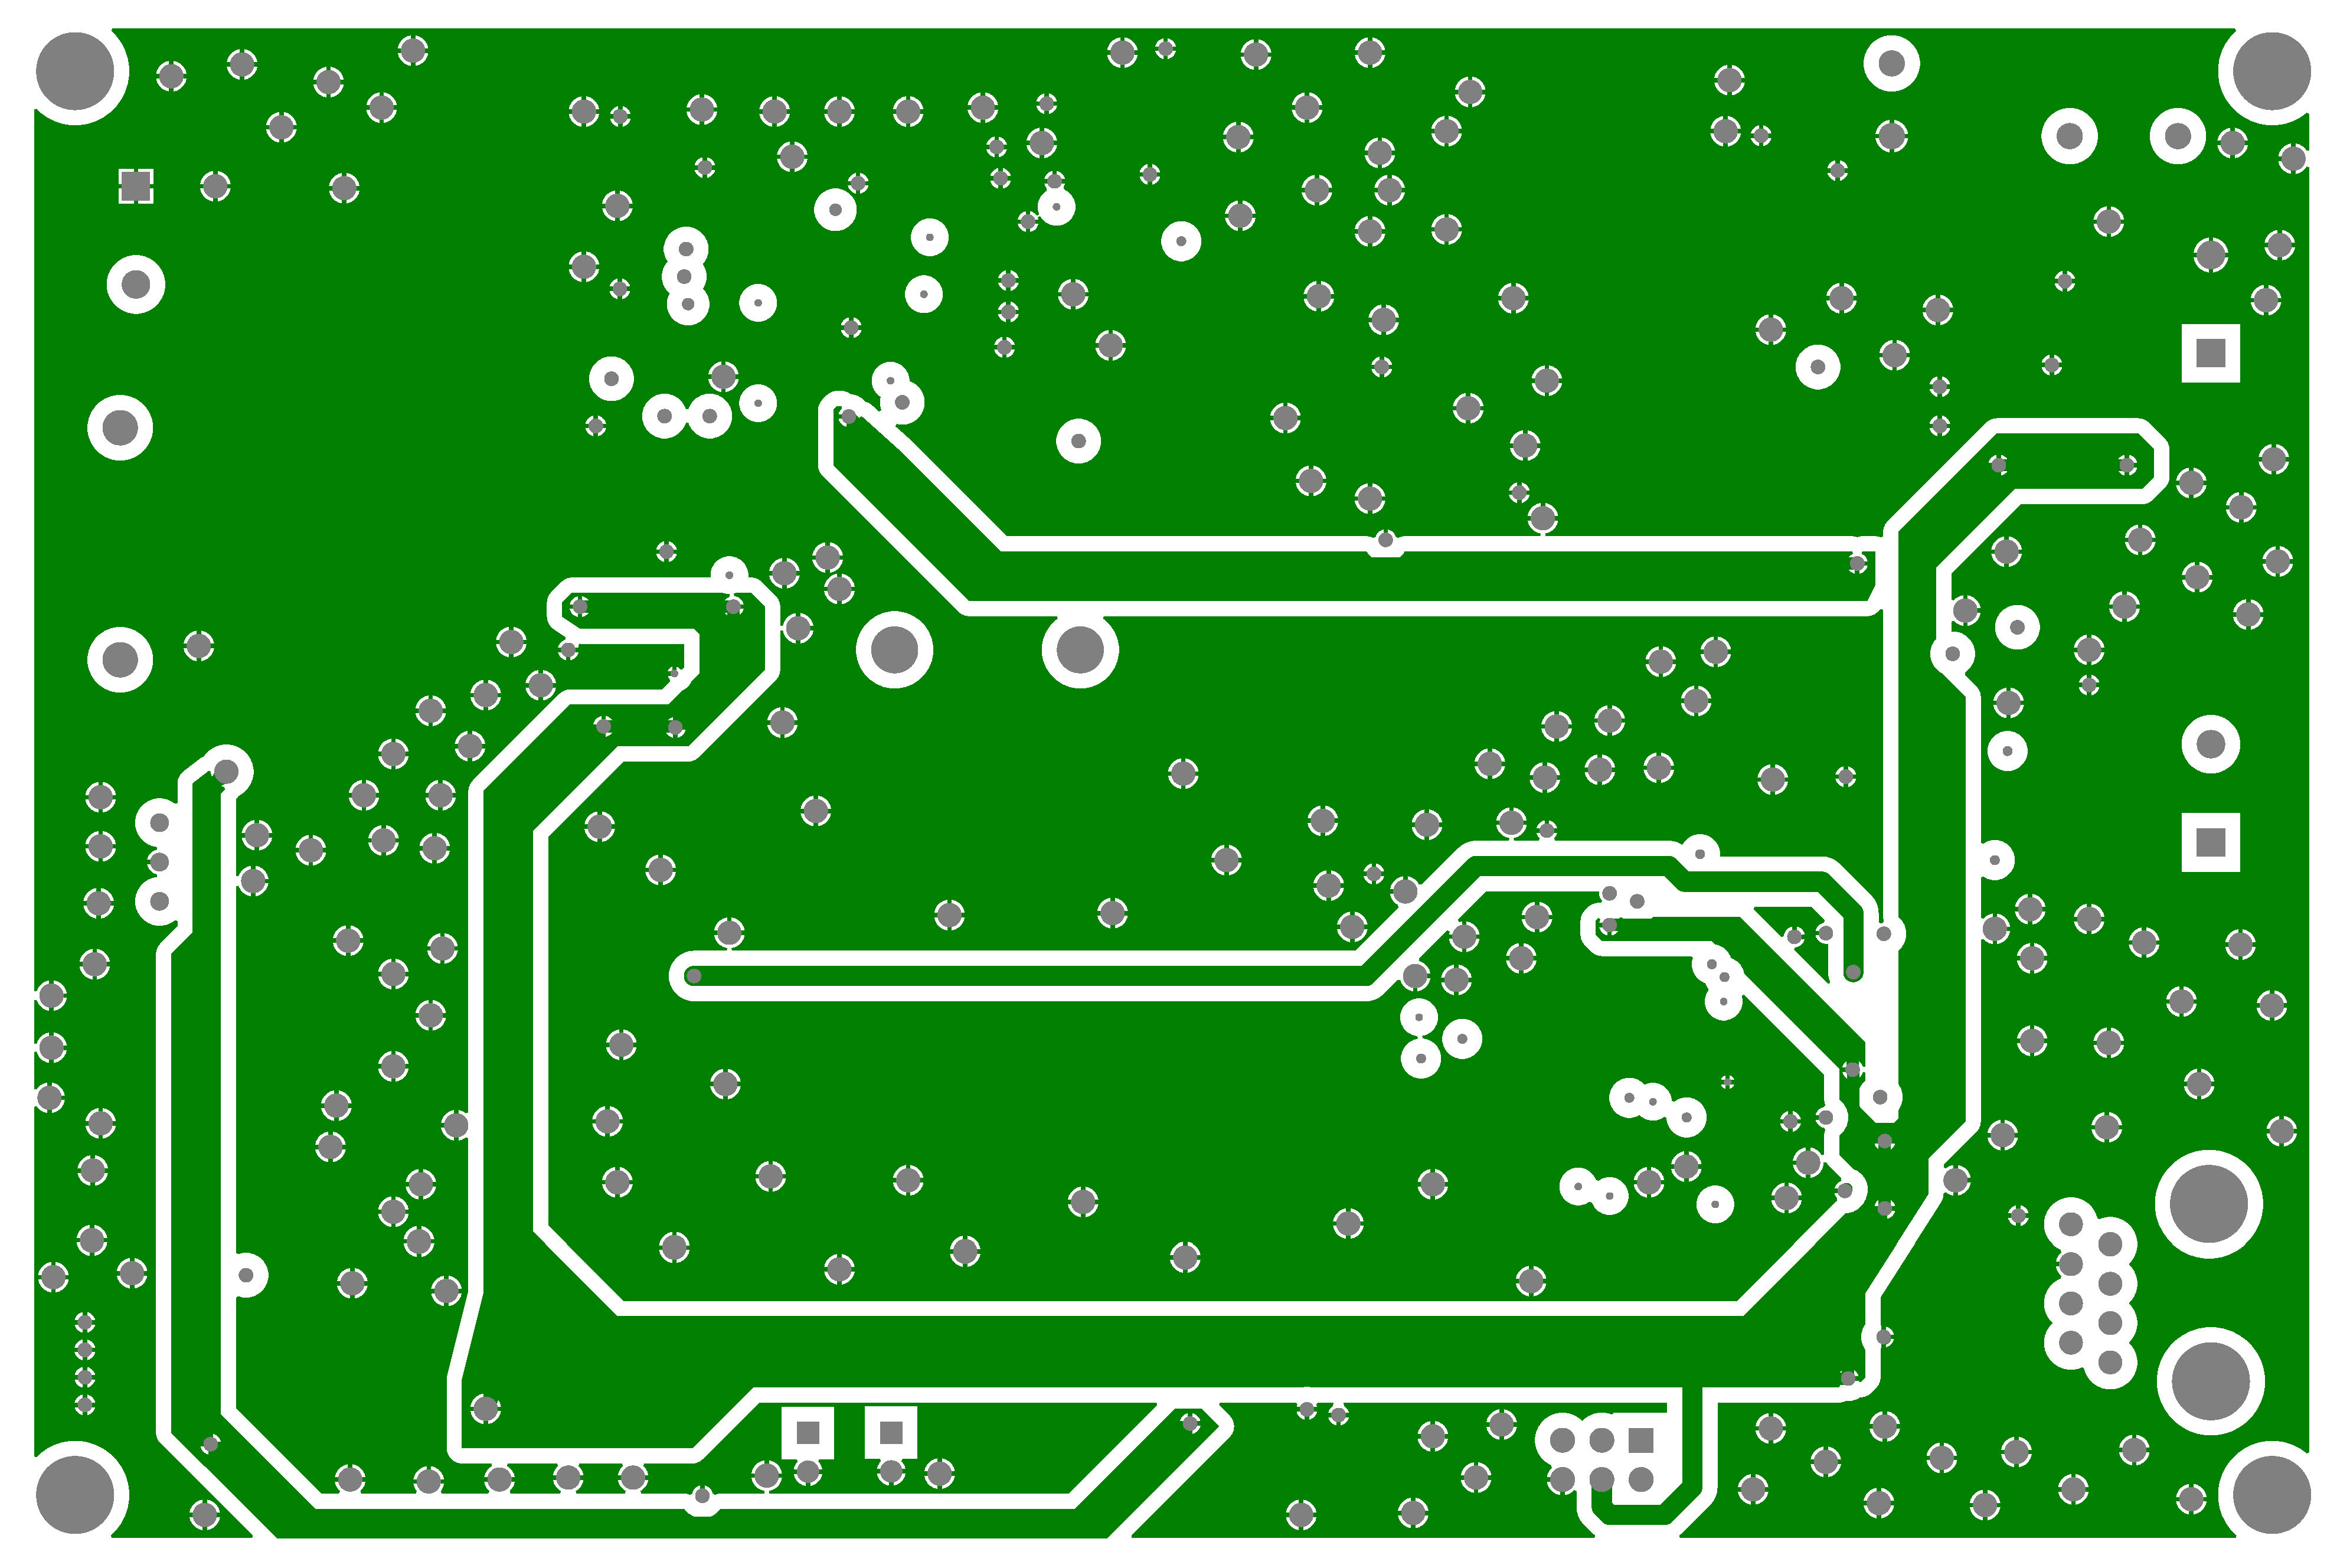
\includegraphics[width = 15cm]{zalaczniki/zasilacz/Zasilacz_regulowany_Strona_10.jpg}
        \caption{Warstwa wewnętrzna 2 PCB.}
    \end{center}
\end{figure}

\begin{figure}
    \begin{center}
        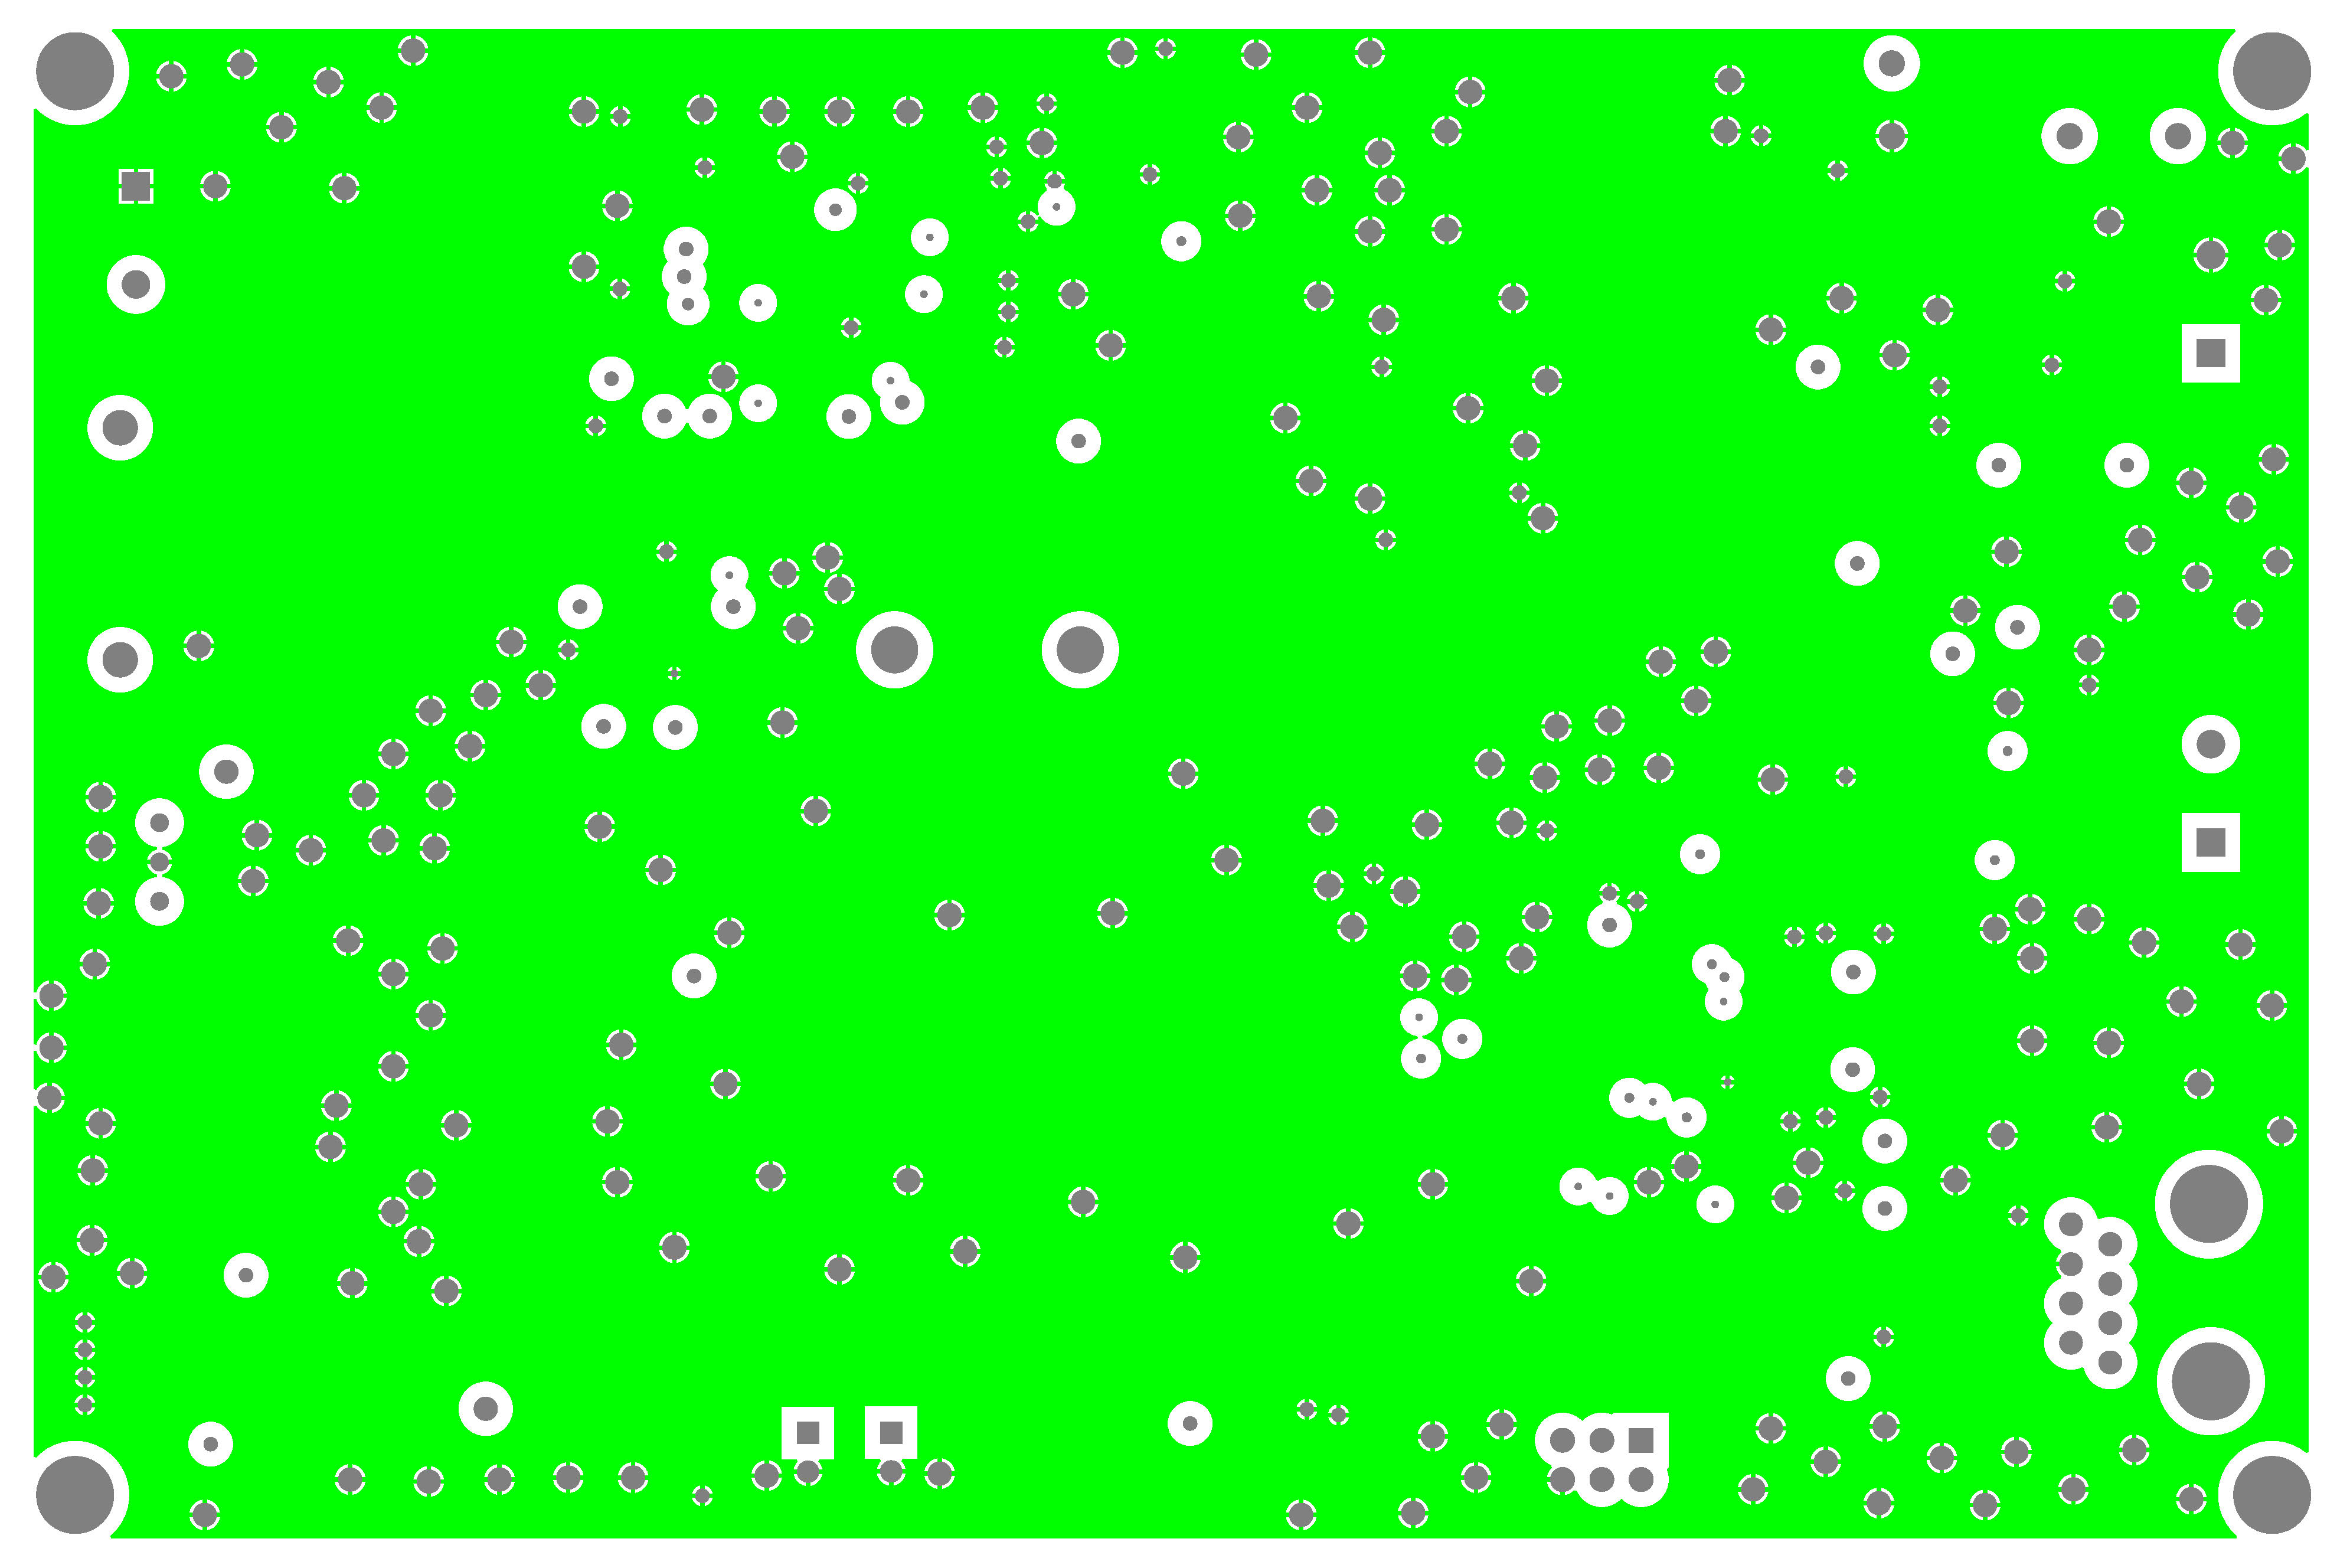
\includegraphics[width = 15cm]{zalaczniki/zasilacz/Zasilacz_regulowany_Strona_11.jpg}
        \caption{Warstwa wewnętrzna 2 PCB.}
    \end{center}
\end{figure}

\begin{figure}
    \begin{center}
        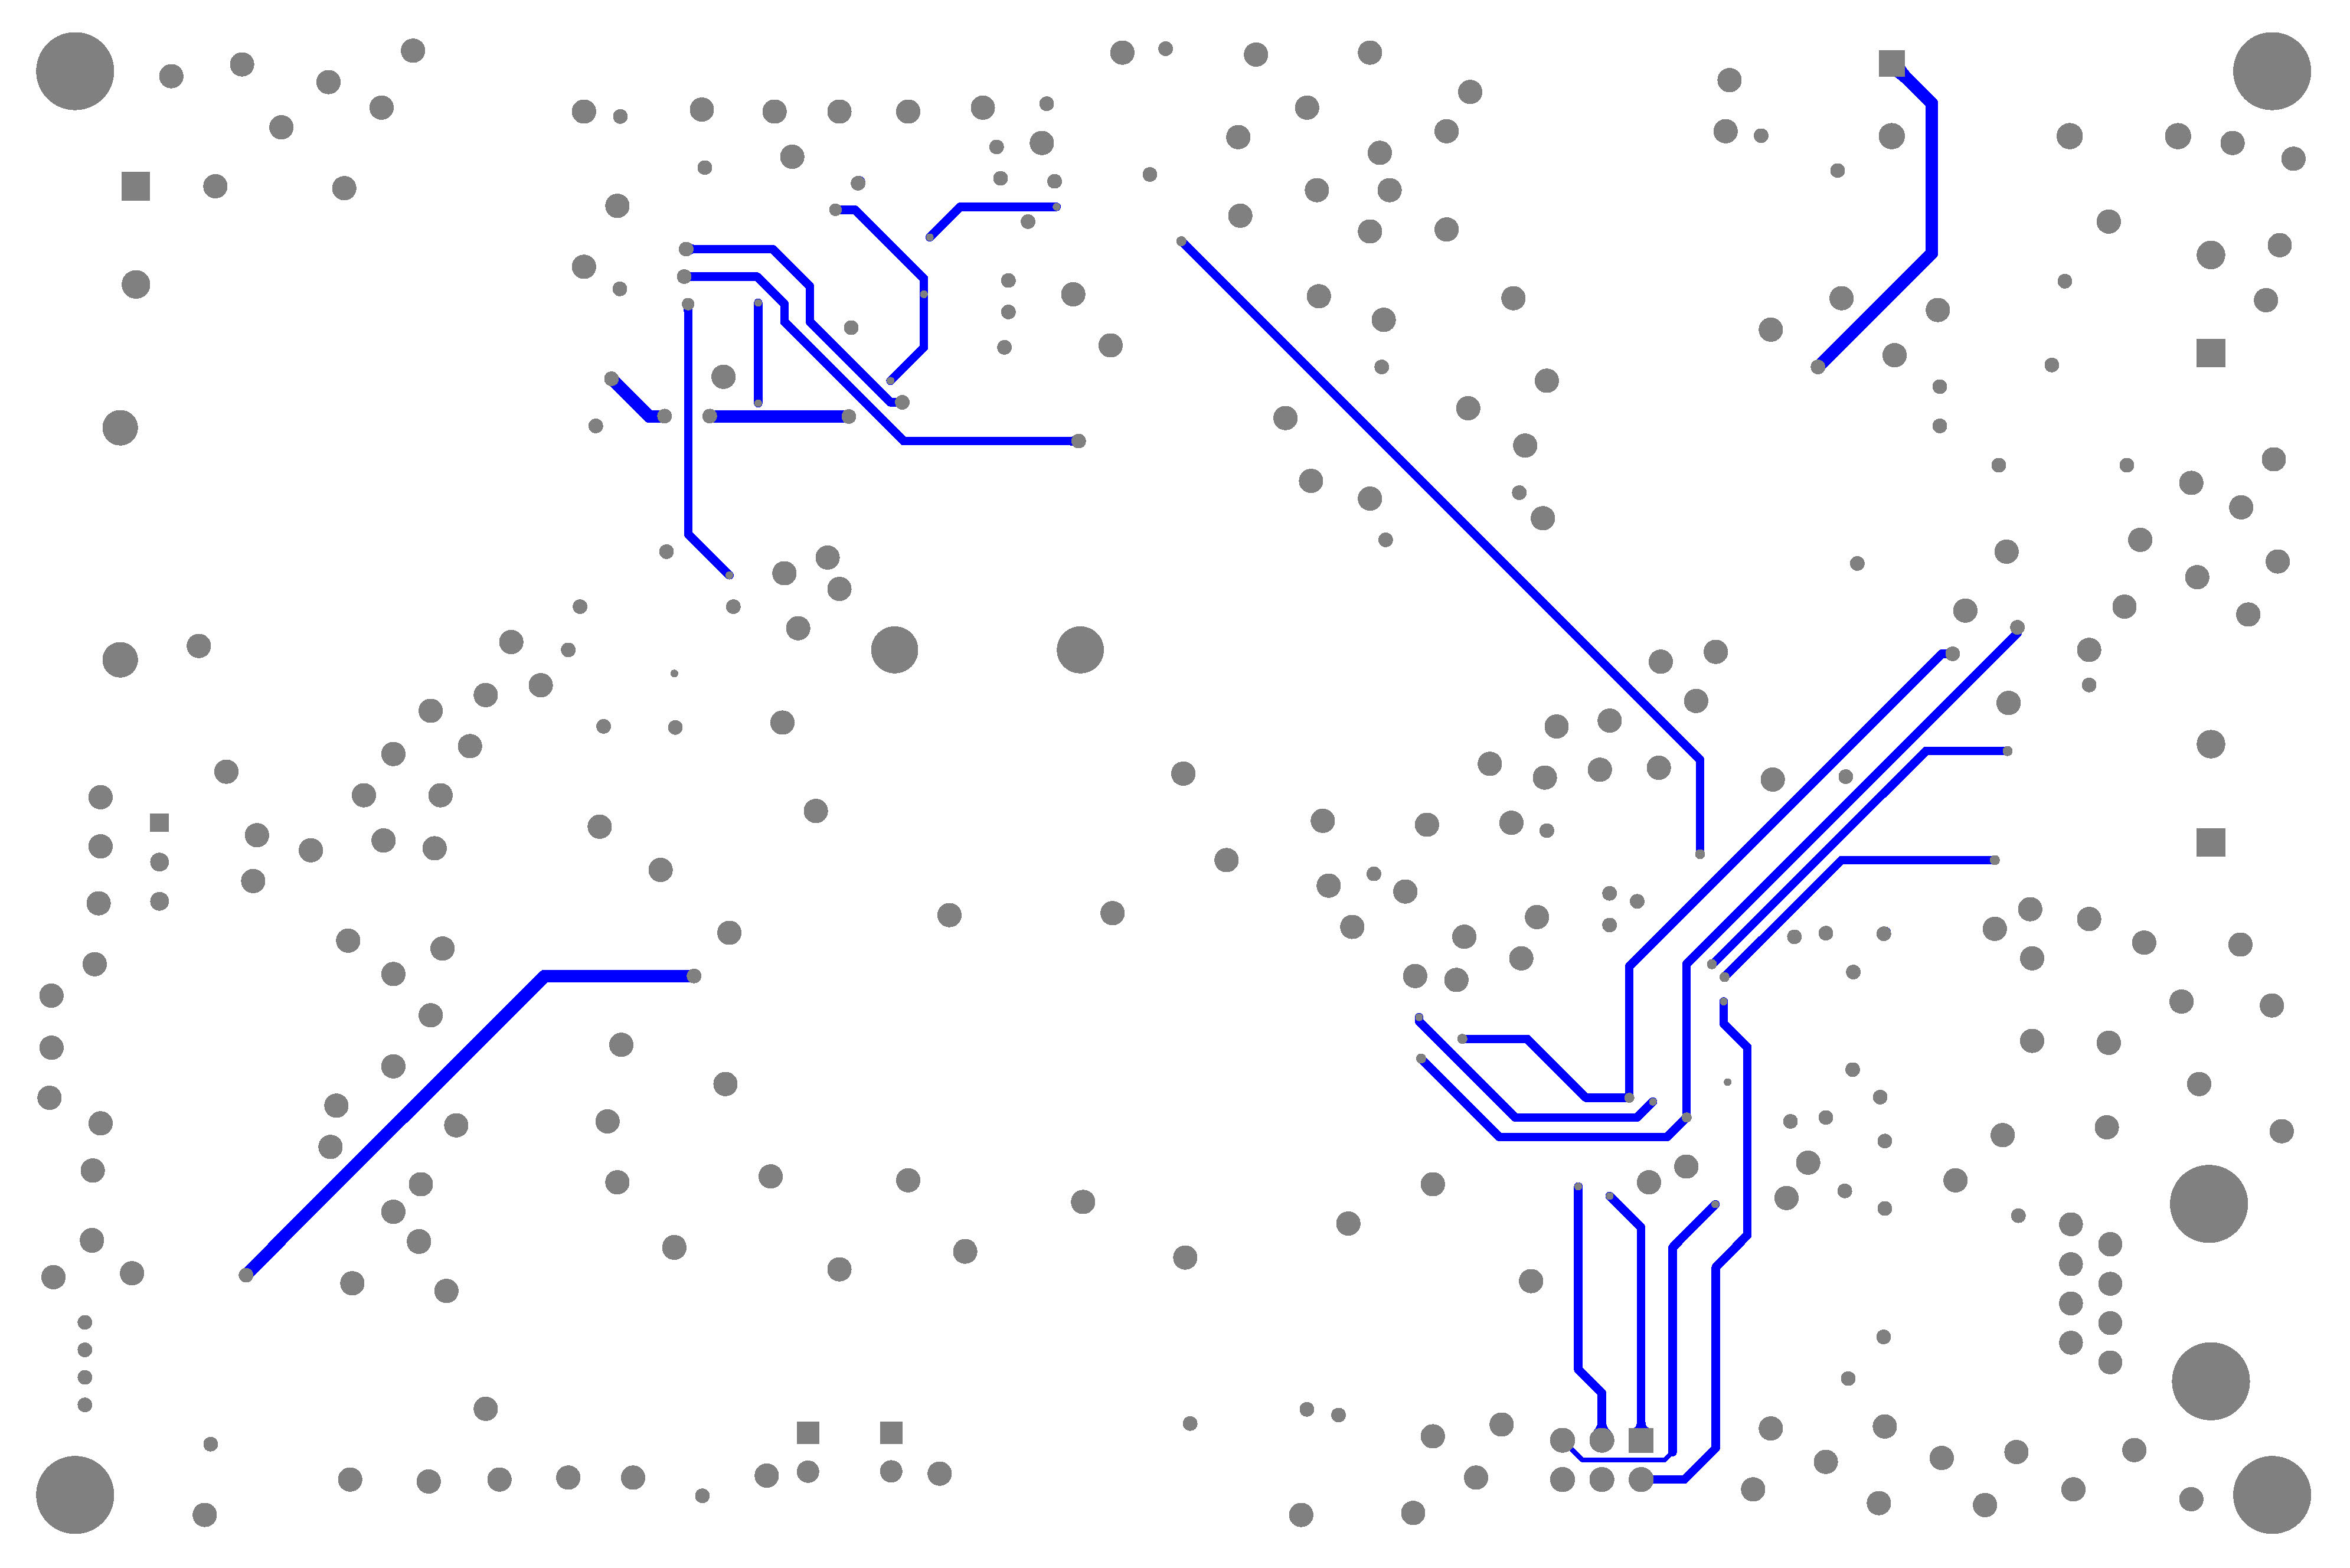
\includegraphics[width = 15cm]{zalaczniki/zasilacz/Zasilacz_regulowany_Strona_12.jpg}
        \caption{Warstwa dolna PCB.}
    \end{center}
\end{figure}


\nopagebreak

\chapter{Moduł obciążenia aktywnego}


\begin{figure}[h!]
    \begin{center}
        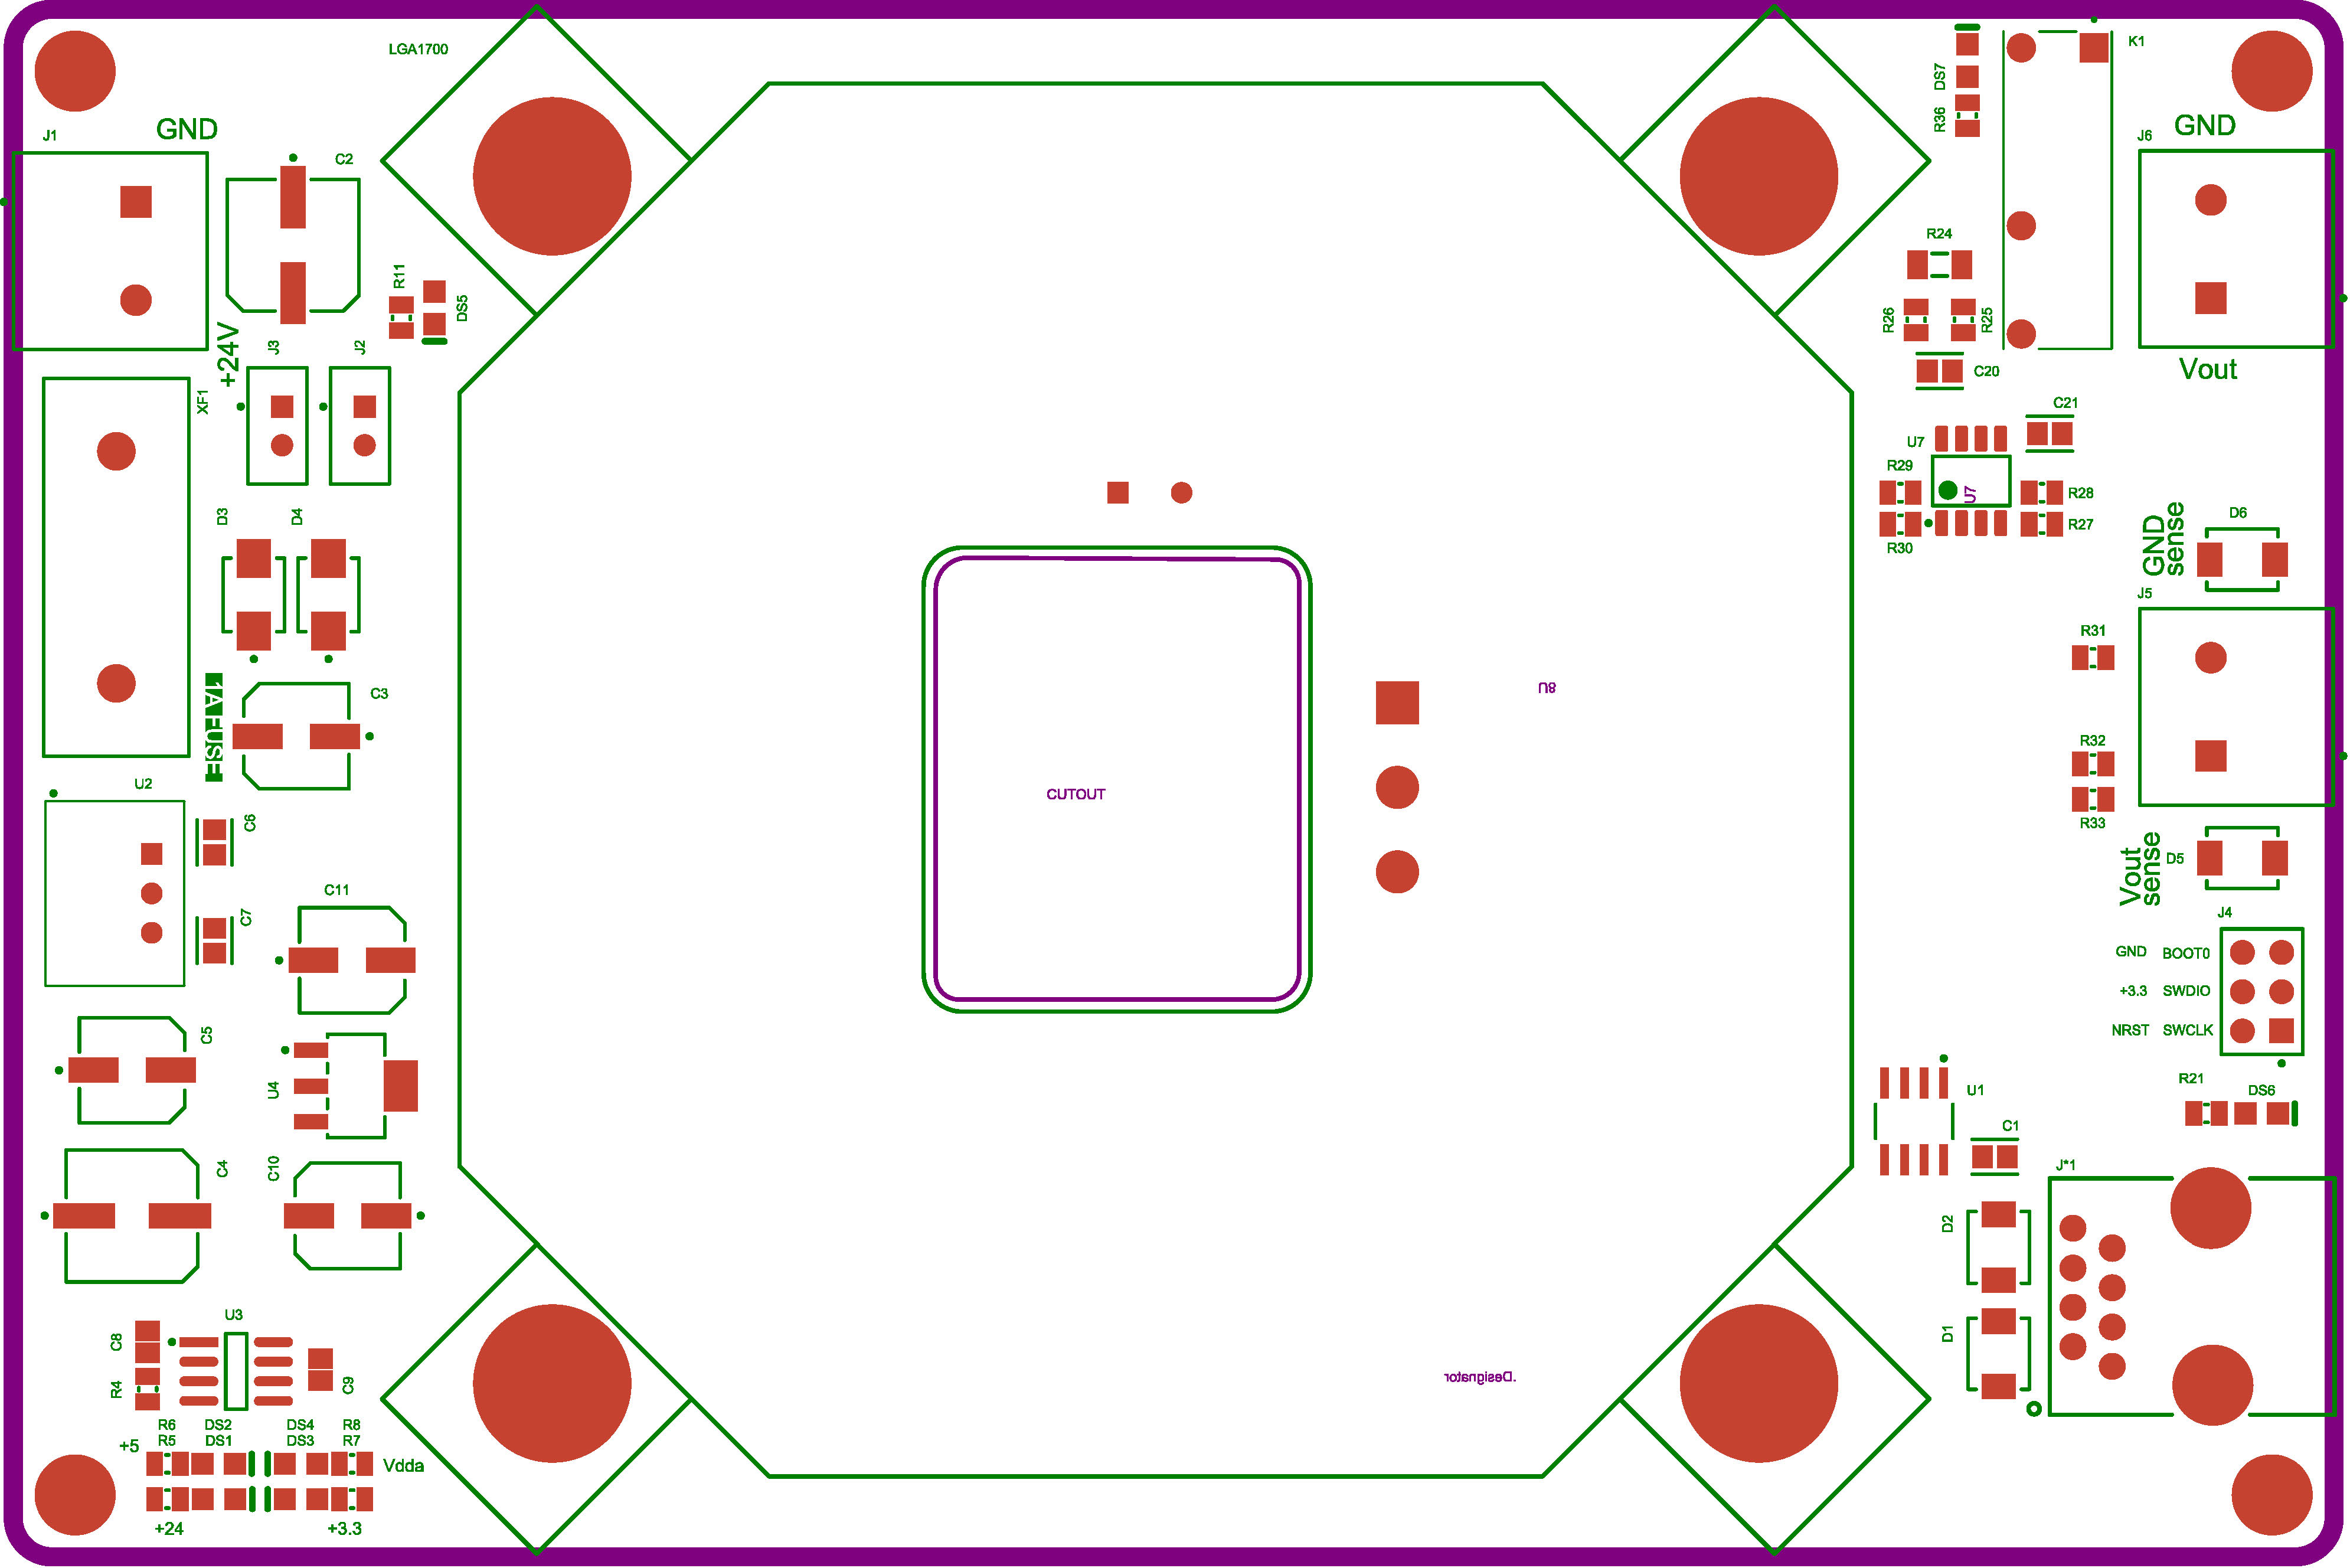
\includegraphics[width = 17cm]{zalaczniki/obciazenie/Obciążenie_aktywne_Strona_13.jpg}
        \caption{Widok warstwy opisowej PCB.}
    \end{center}
\end{figure}

\begin{sidewaysfigure}
    \begin{center}
        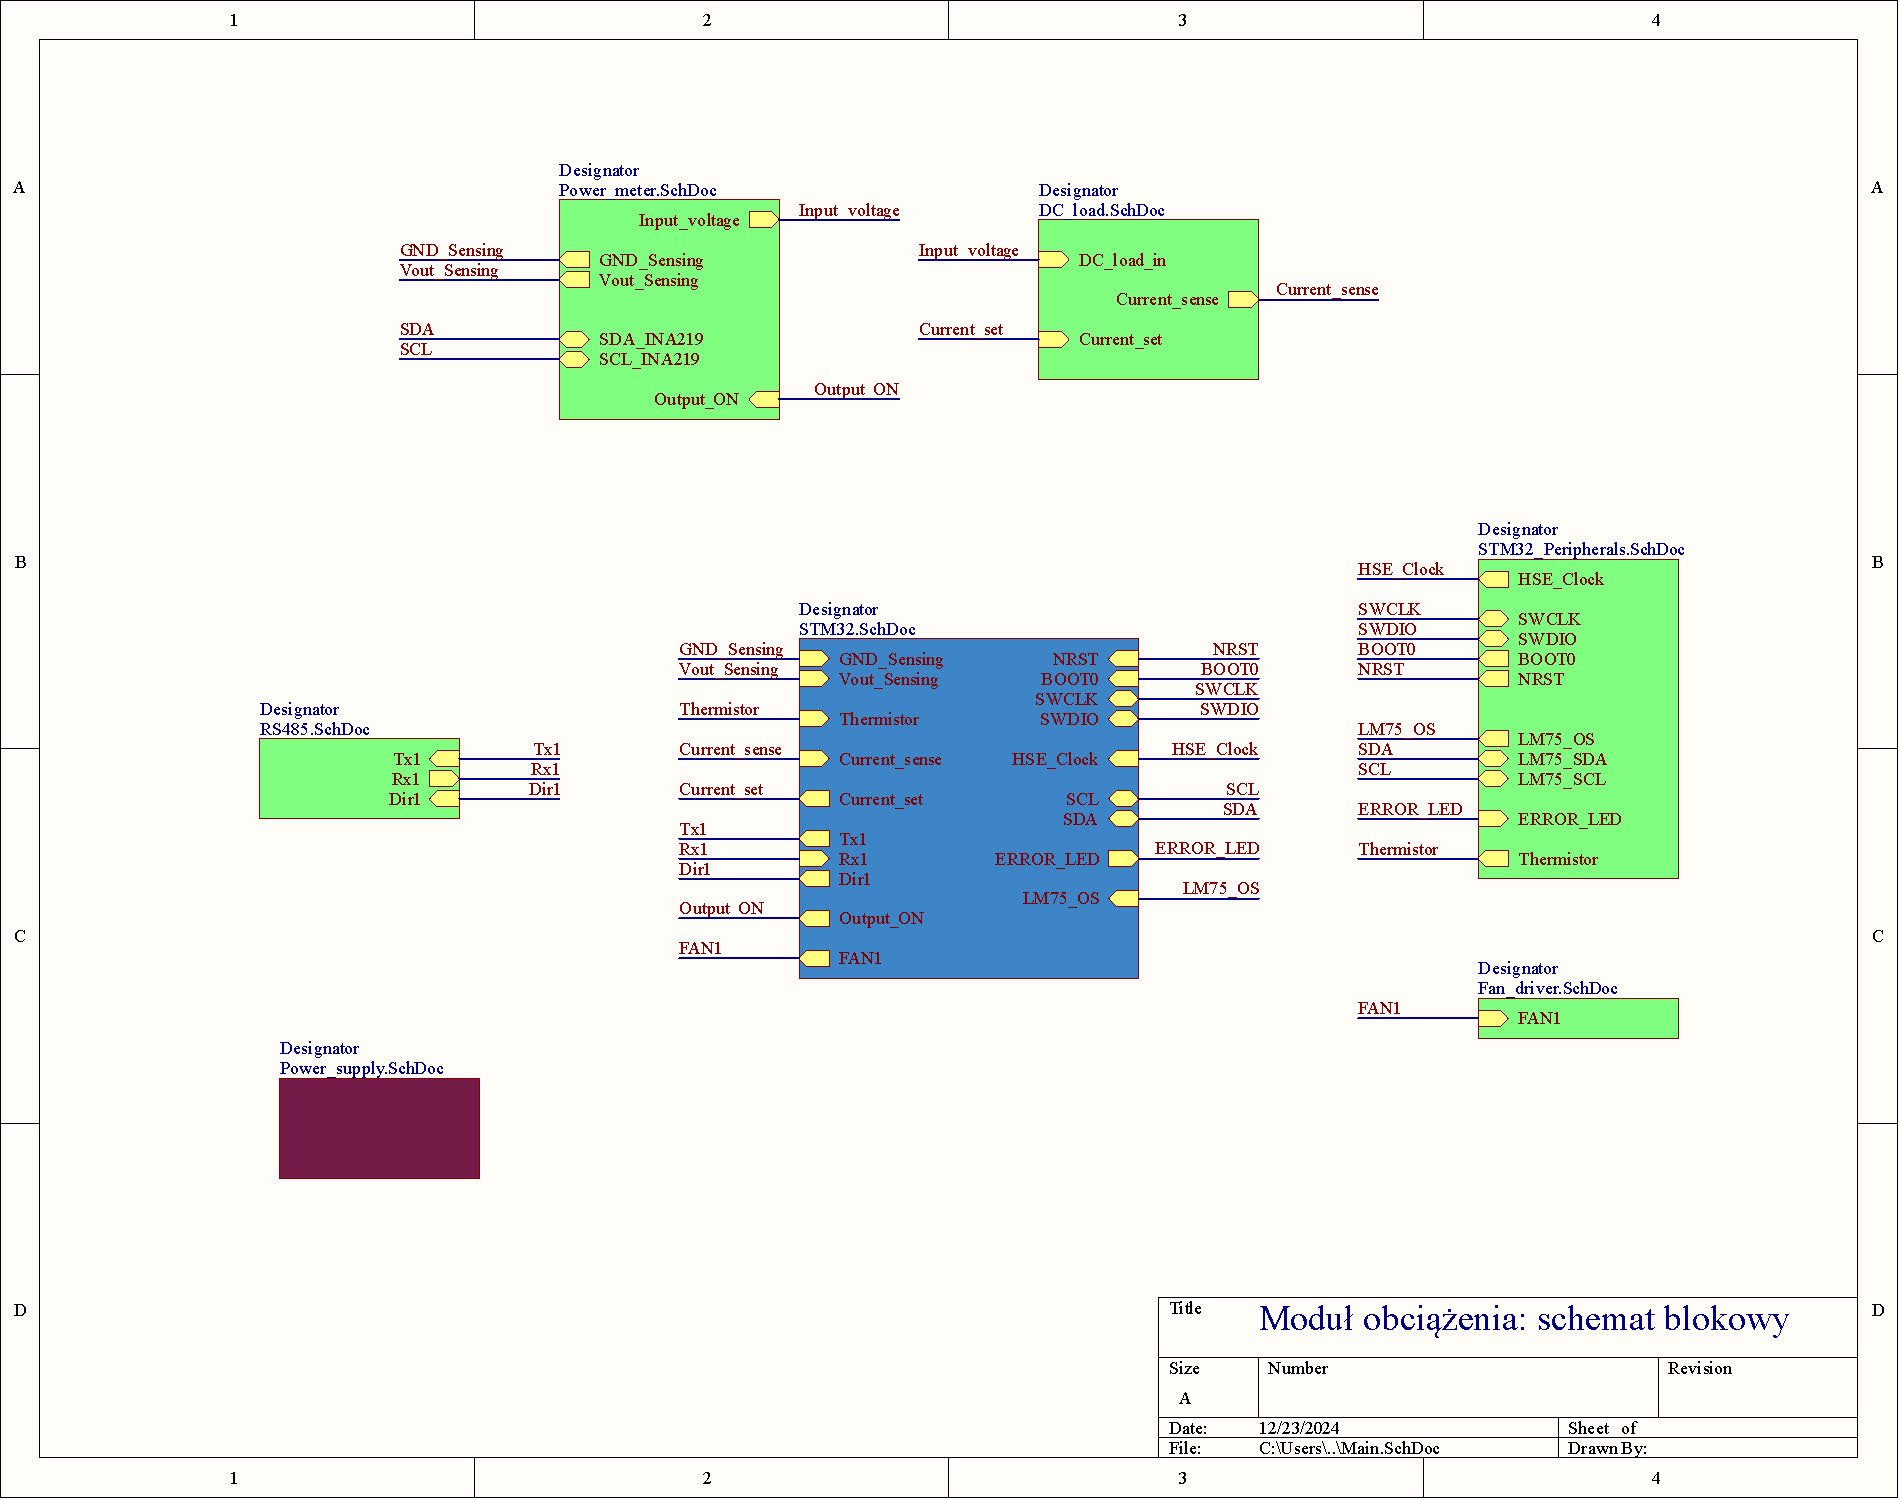
\includegraphics[width = 21cm]{zalaczniki/obciazenie/Obciążenie_aktywne_Strona_01.jpg}
        \caption{Schemat blokowy modułu obciążenia aktywnego.}
    \end{center}
\end{sidewaysfigure}

\begin{sidewaysfigure}
    \begin{center}
        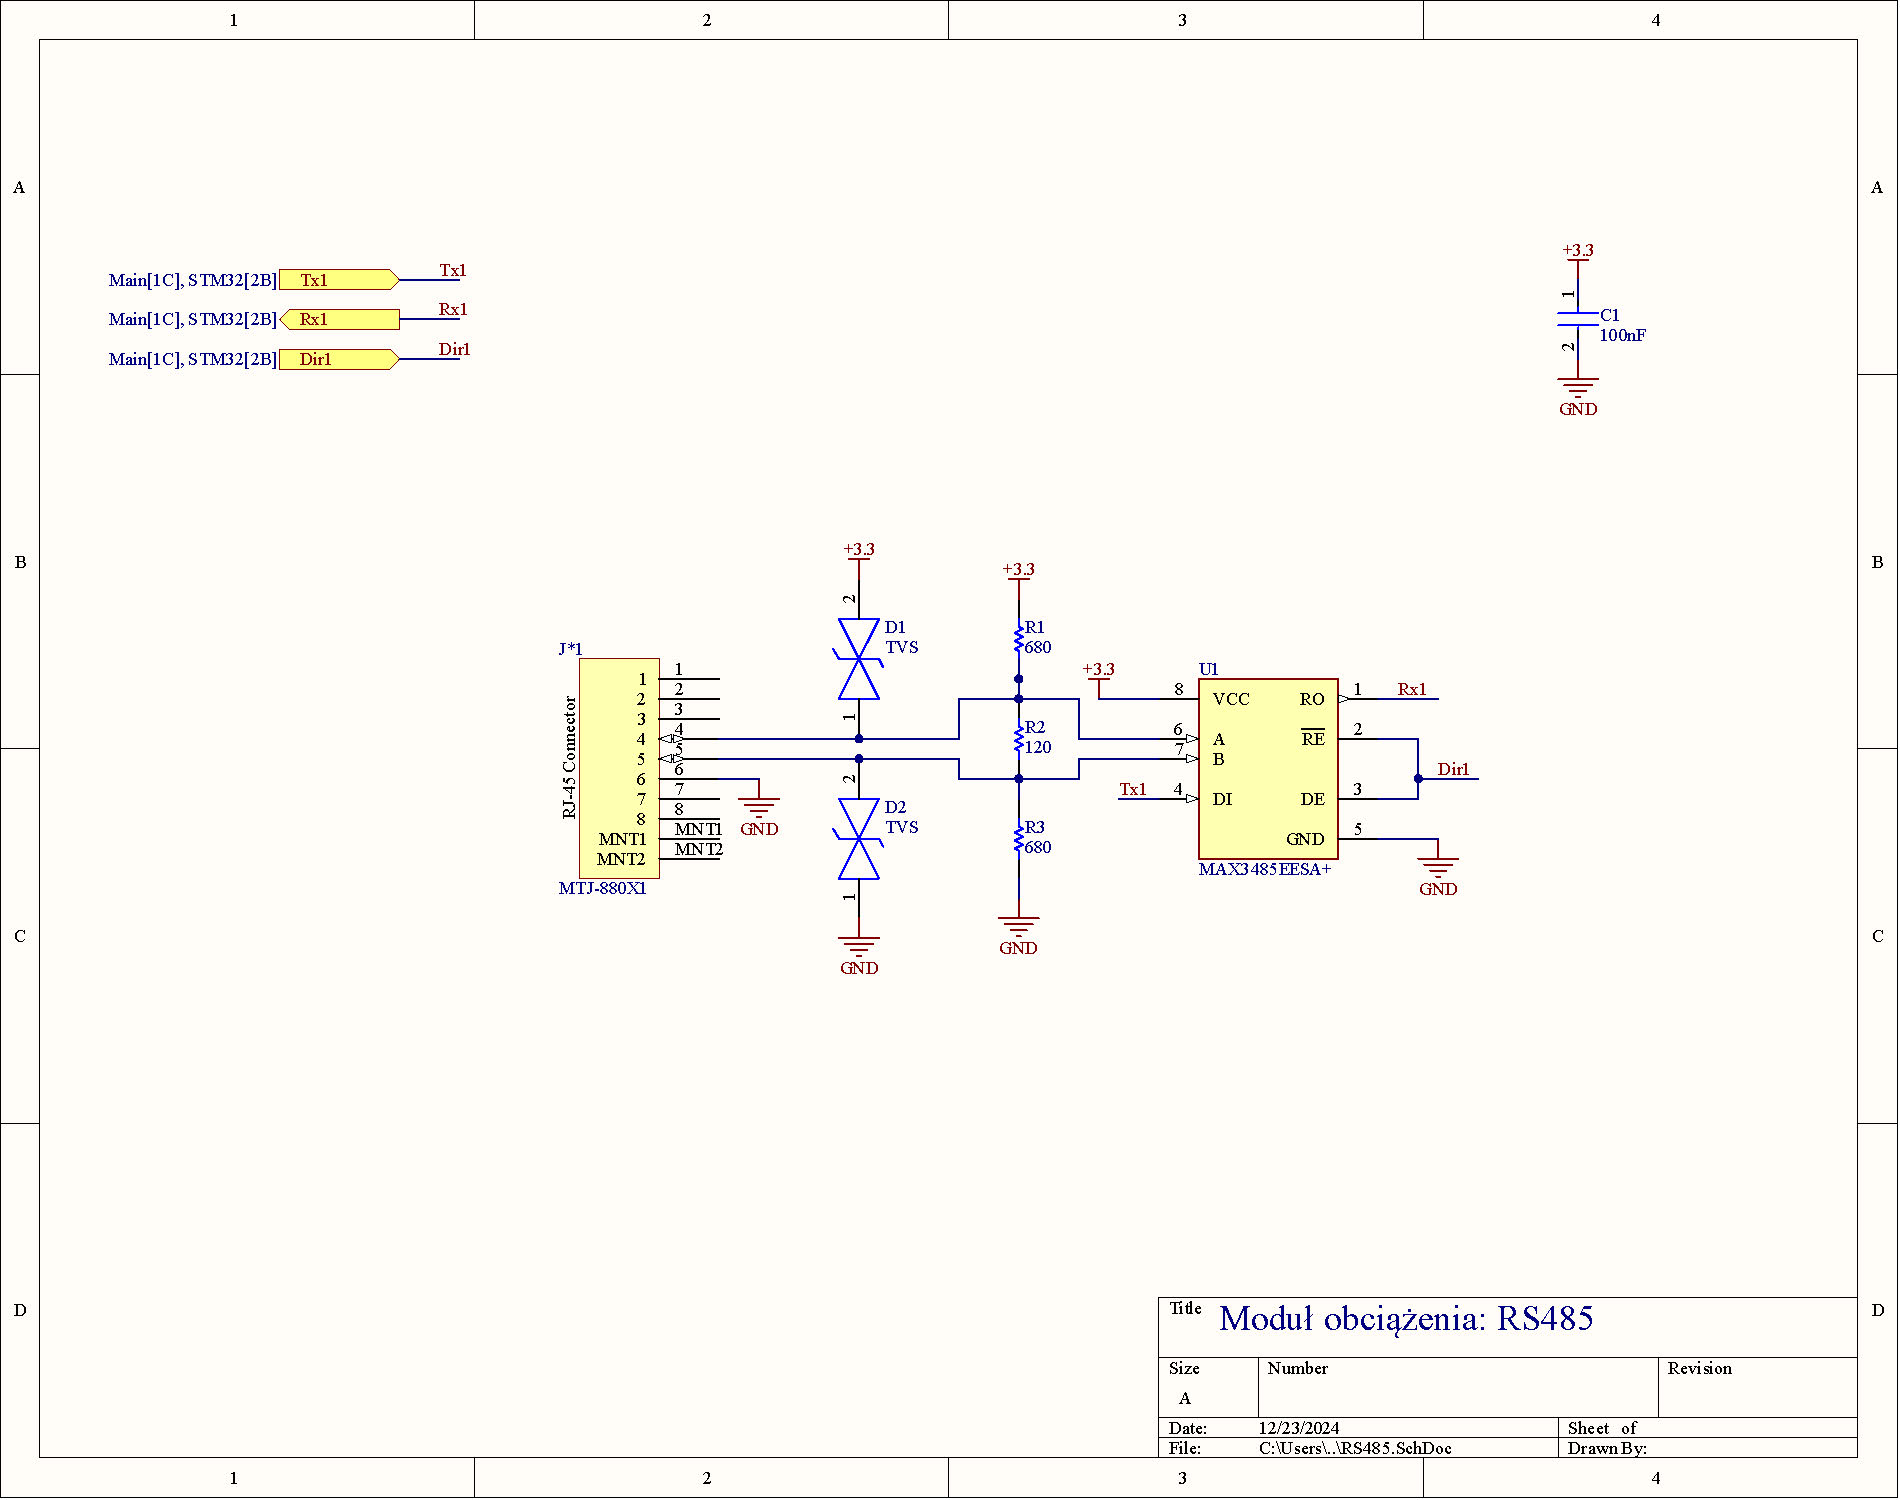
\includegraphics[width = 21cm]{zalaczniki/obciazenie/Obciążenie_aktywne_Strona_02.jpg}
        \caption{Schemat RS485.}
    \end{center}
\end{sidewaysfigure}

\begin{sidewaysfigure}
    \begin{center}
        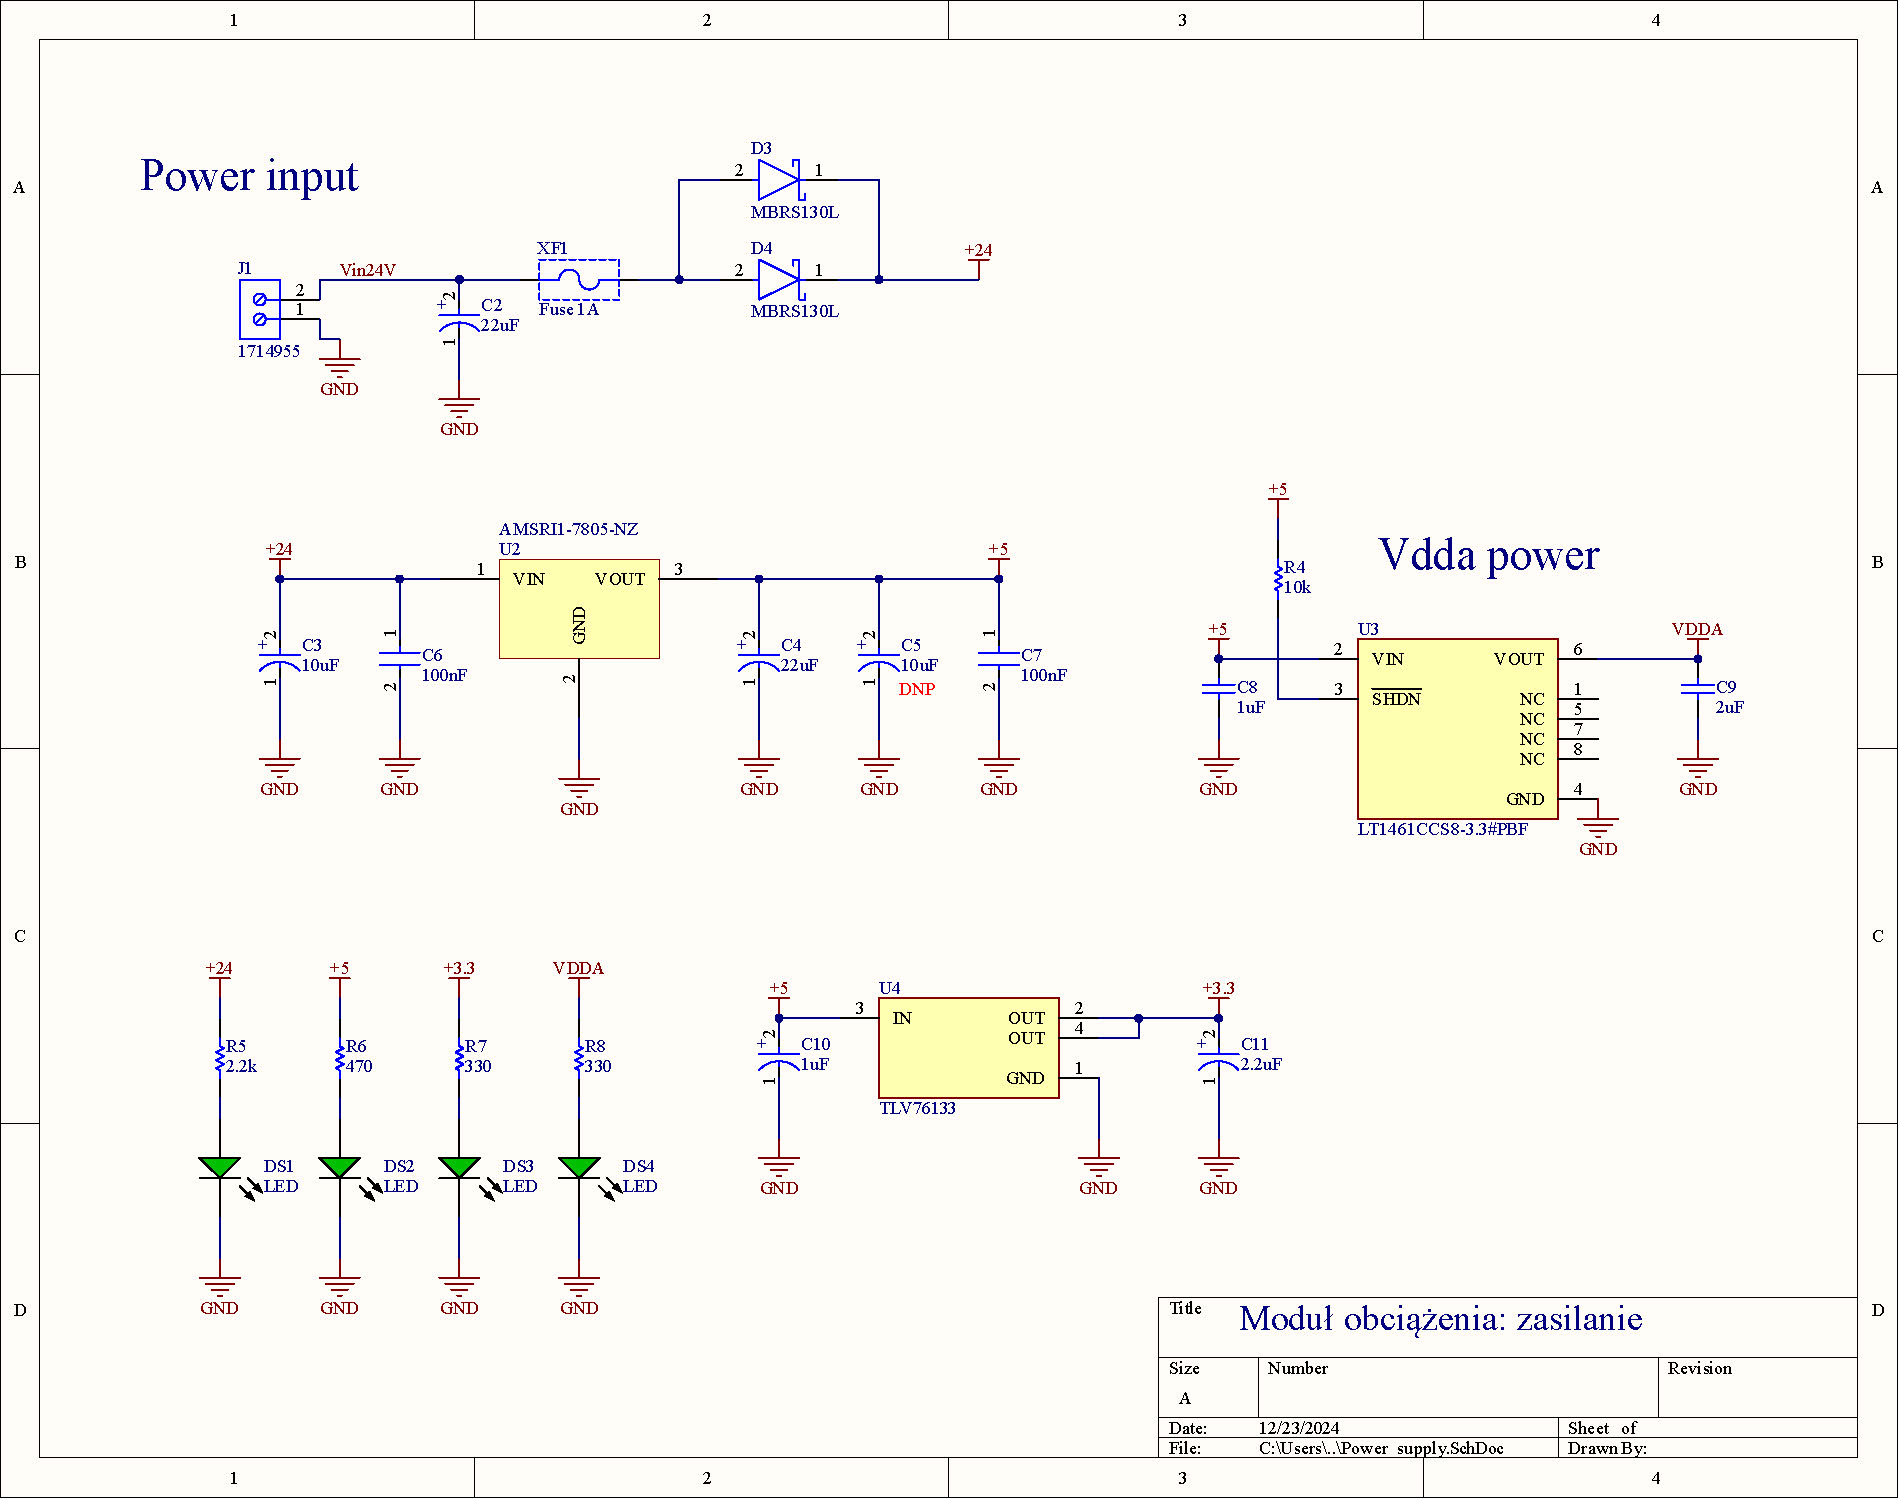
\includegraphics[width = 21cm]{zalaczniki/obciazenie/Obciążenie_aktywne_Strona_03.jpg}
        \caption{Schemat sekcji zasilania.}
    \end{center}
\end{sidewaysfigure}

\begin{sidewaysfigure}
    \begin{center}
        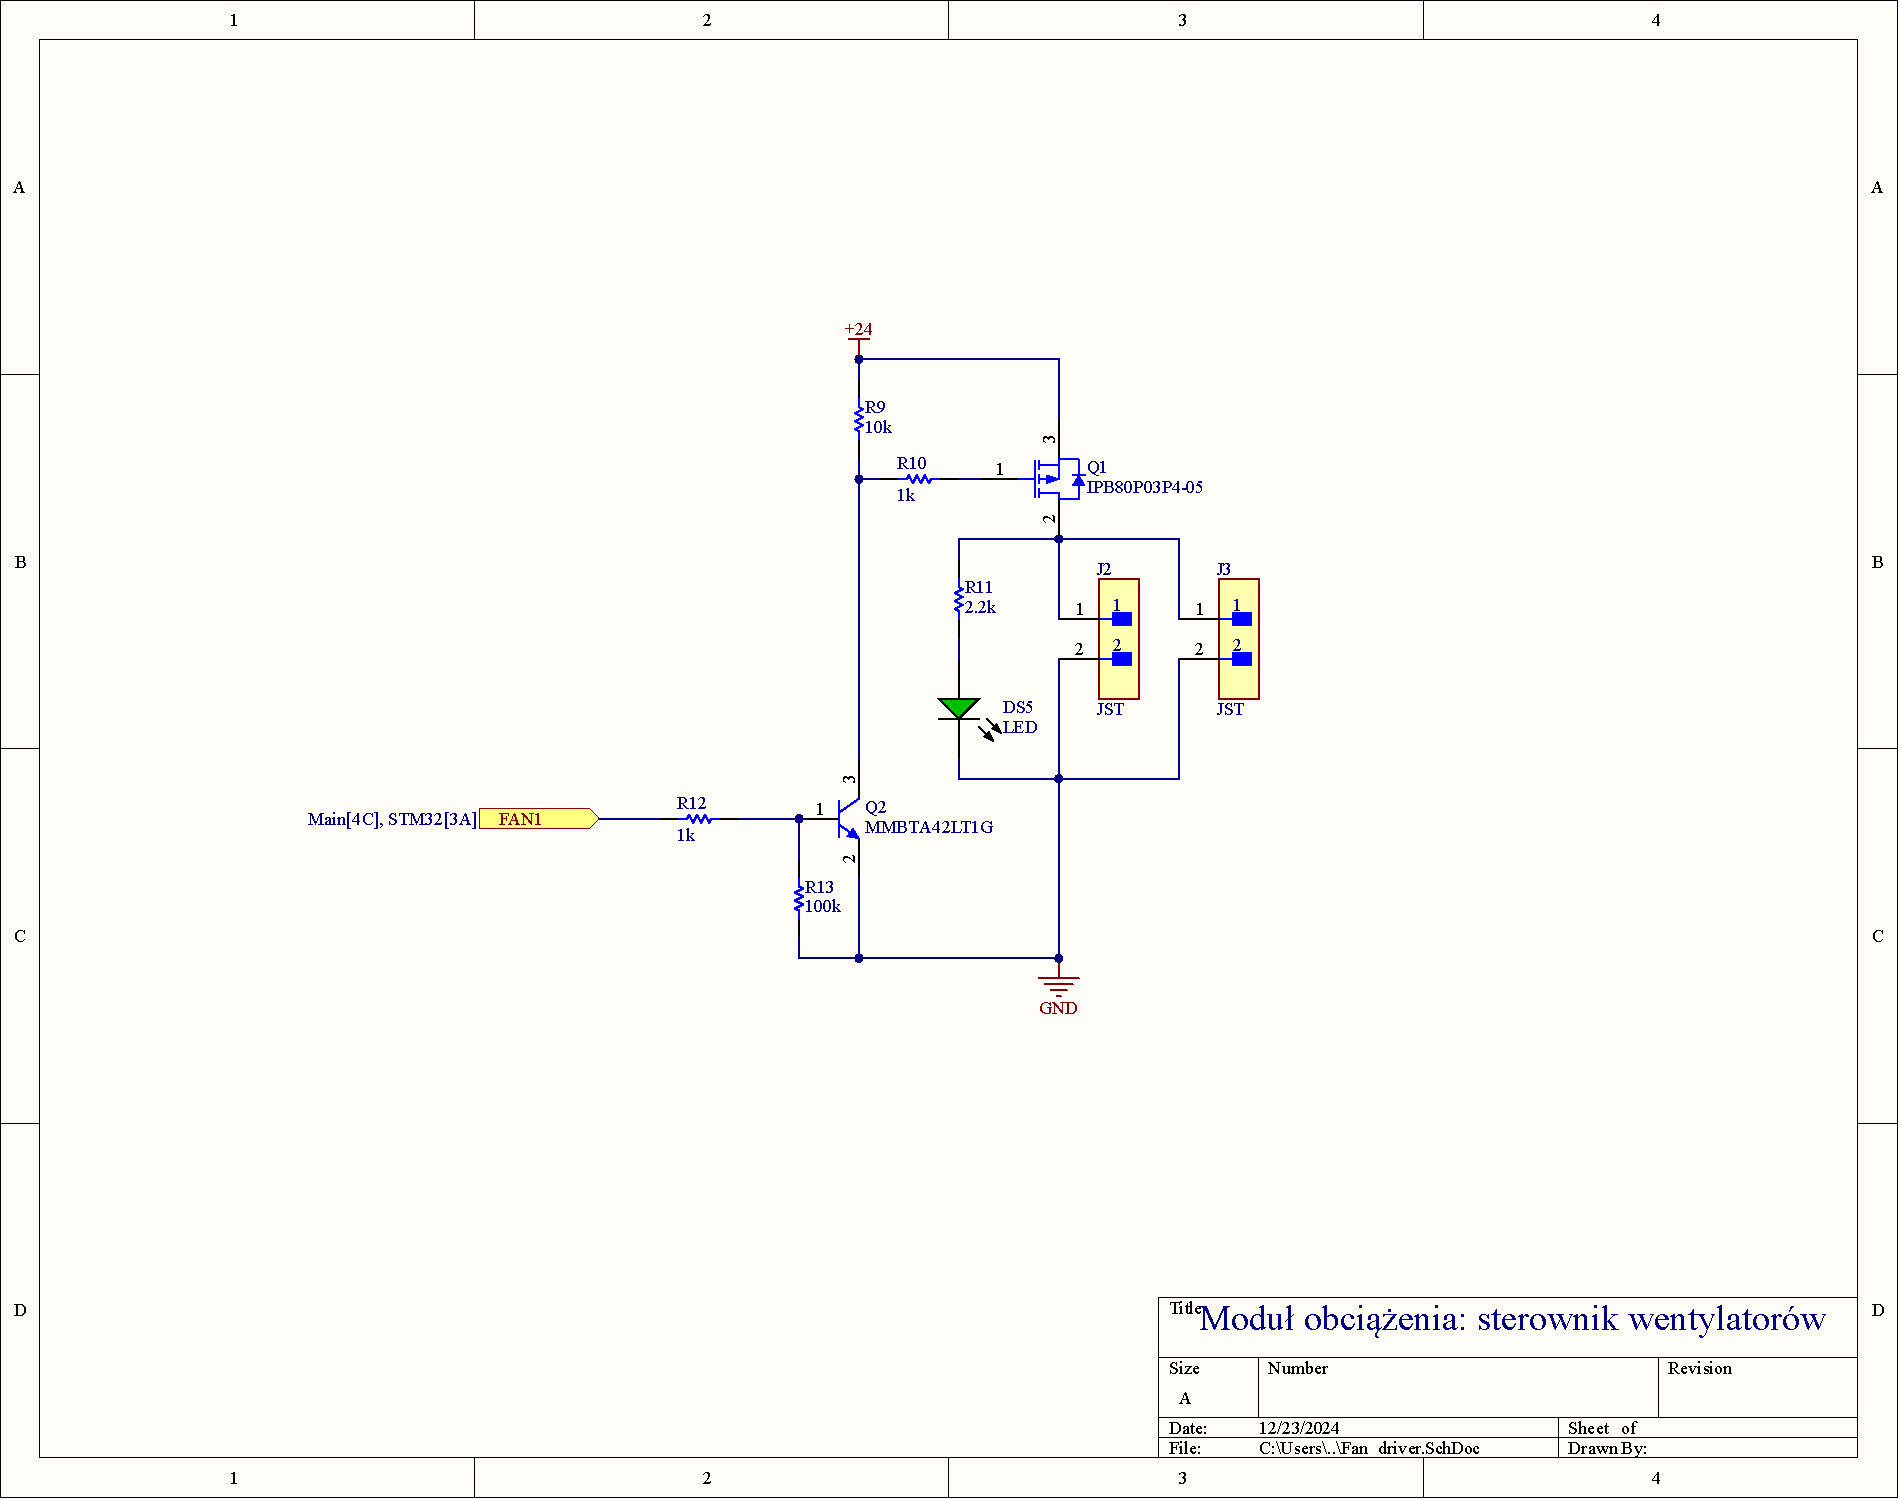
\includegraphics[width = 21cm]{zalaczniki/obciazenie/Obciążenie_aktywne_Strona_04.jpg}
        \caption{Schemat sterownika wentylatorów.}
    \end{center}
\end{sidewaysfigure}

\begin{sidewaysfigure}
    \begin{center}
        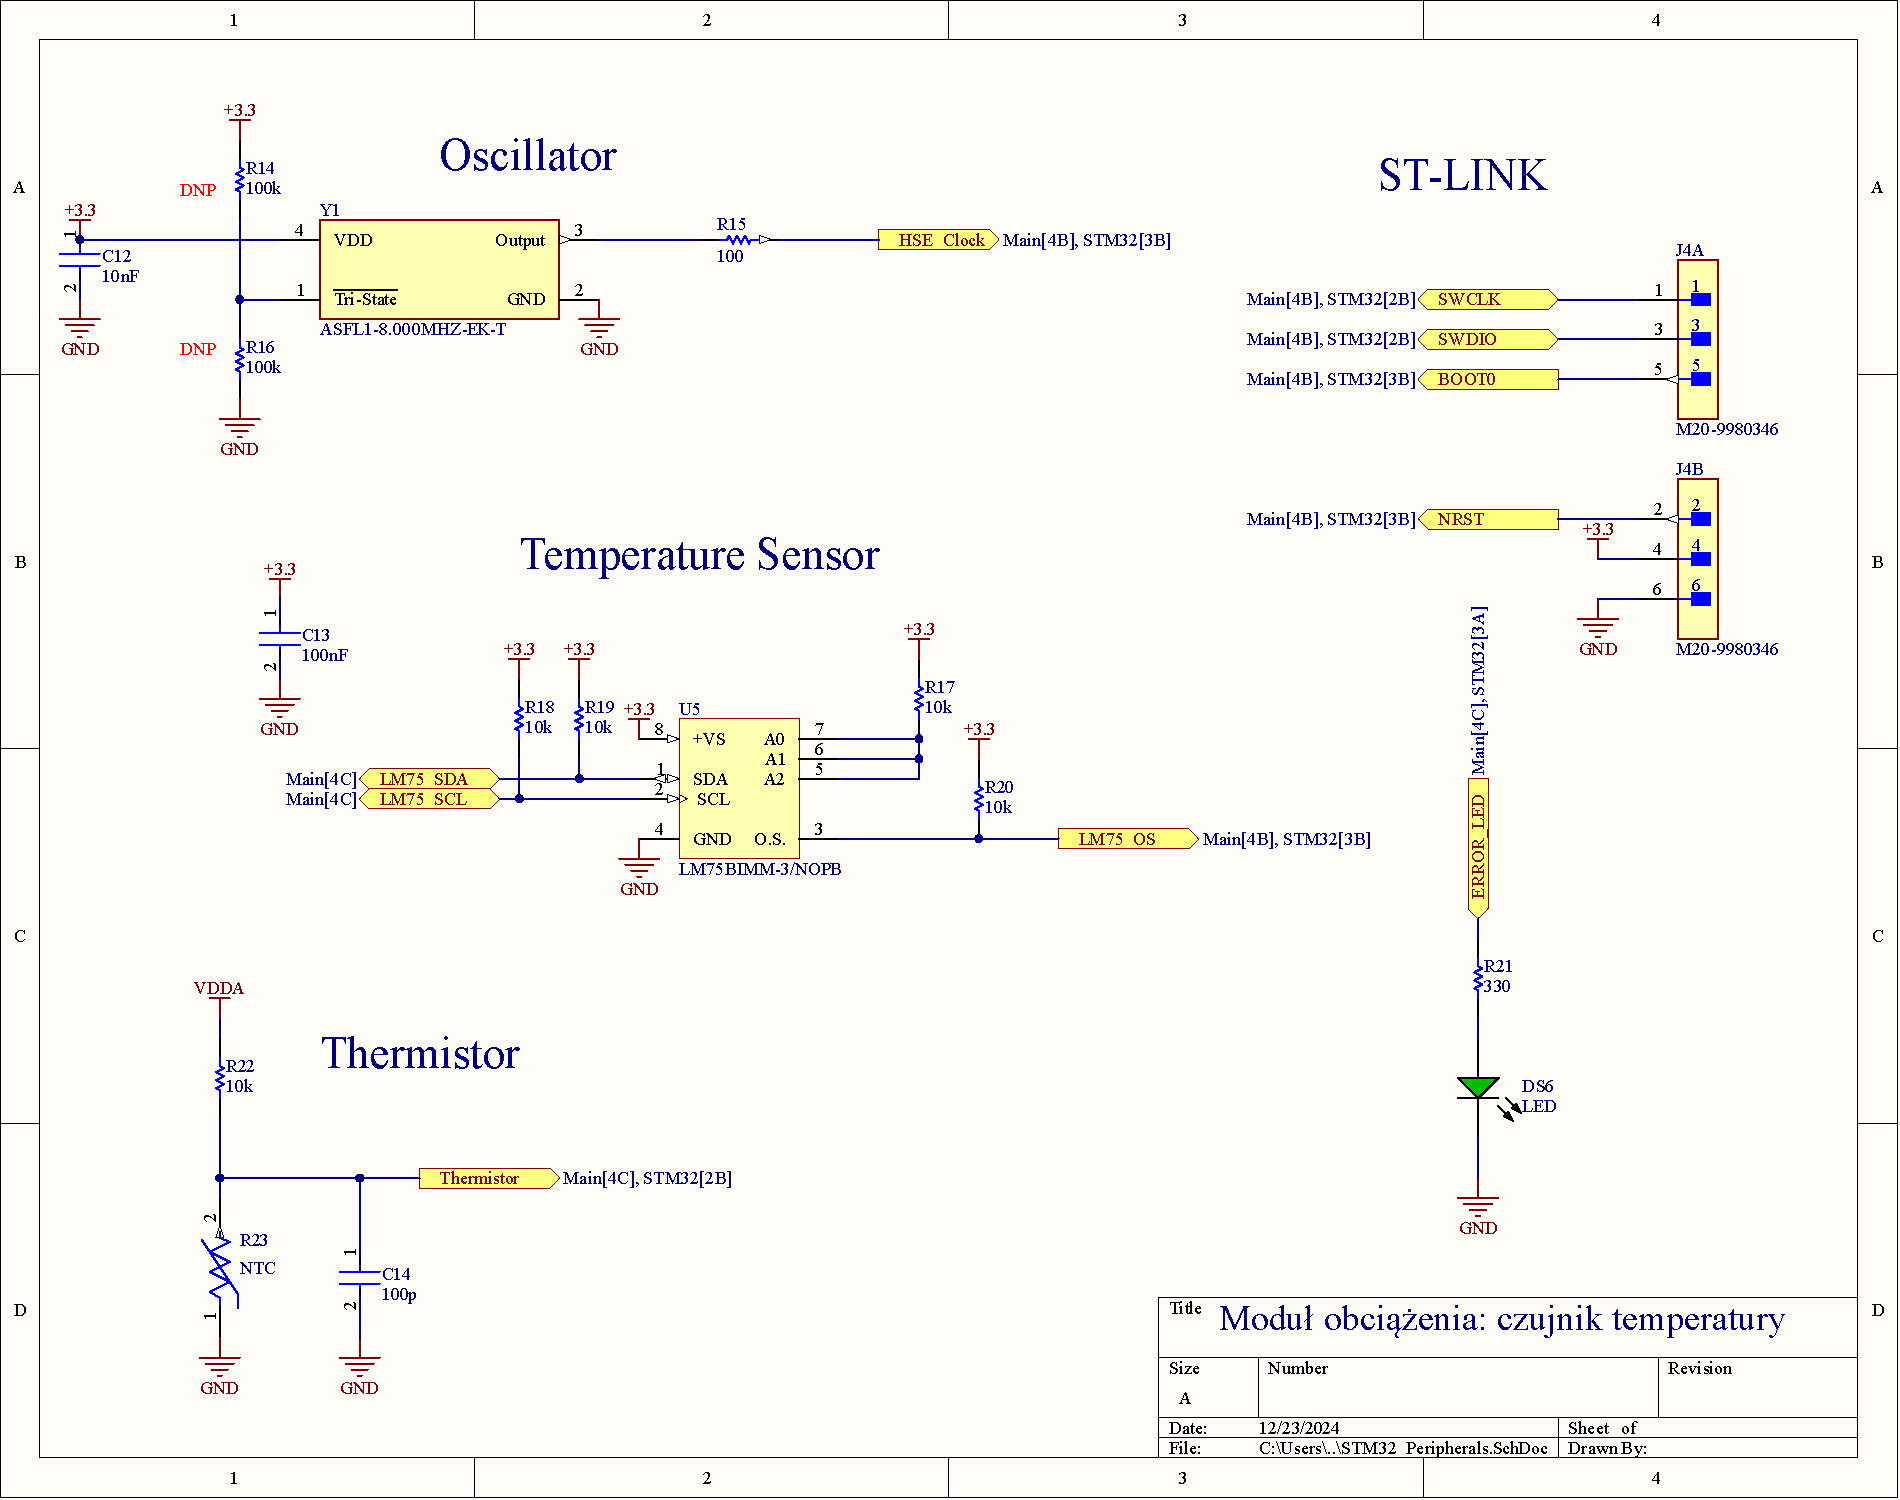
\includegraphics[width = 21cm]{zalaczniki/obciazenie/Obciążenie_aktywne_Strona_05.jpg}
        \caption{Schemat ukladów peryferyjnych.}
    \end{center}
\end{sidewaysfigure}

\begin{sidewaysfigure}
    \begin{center}
        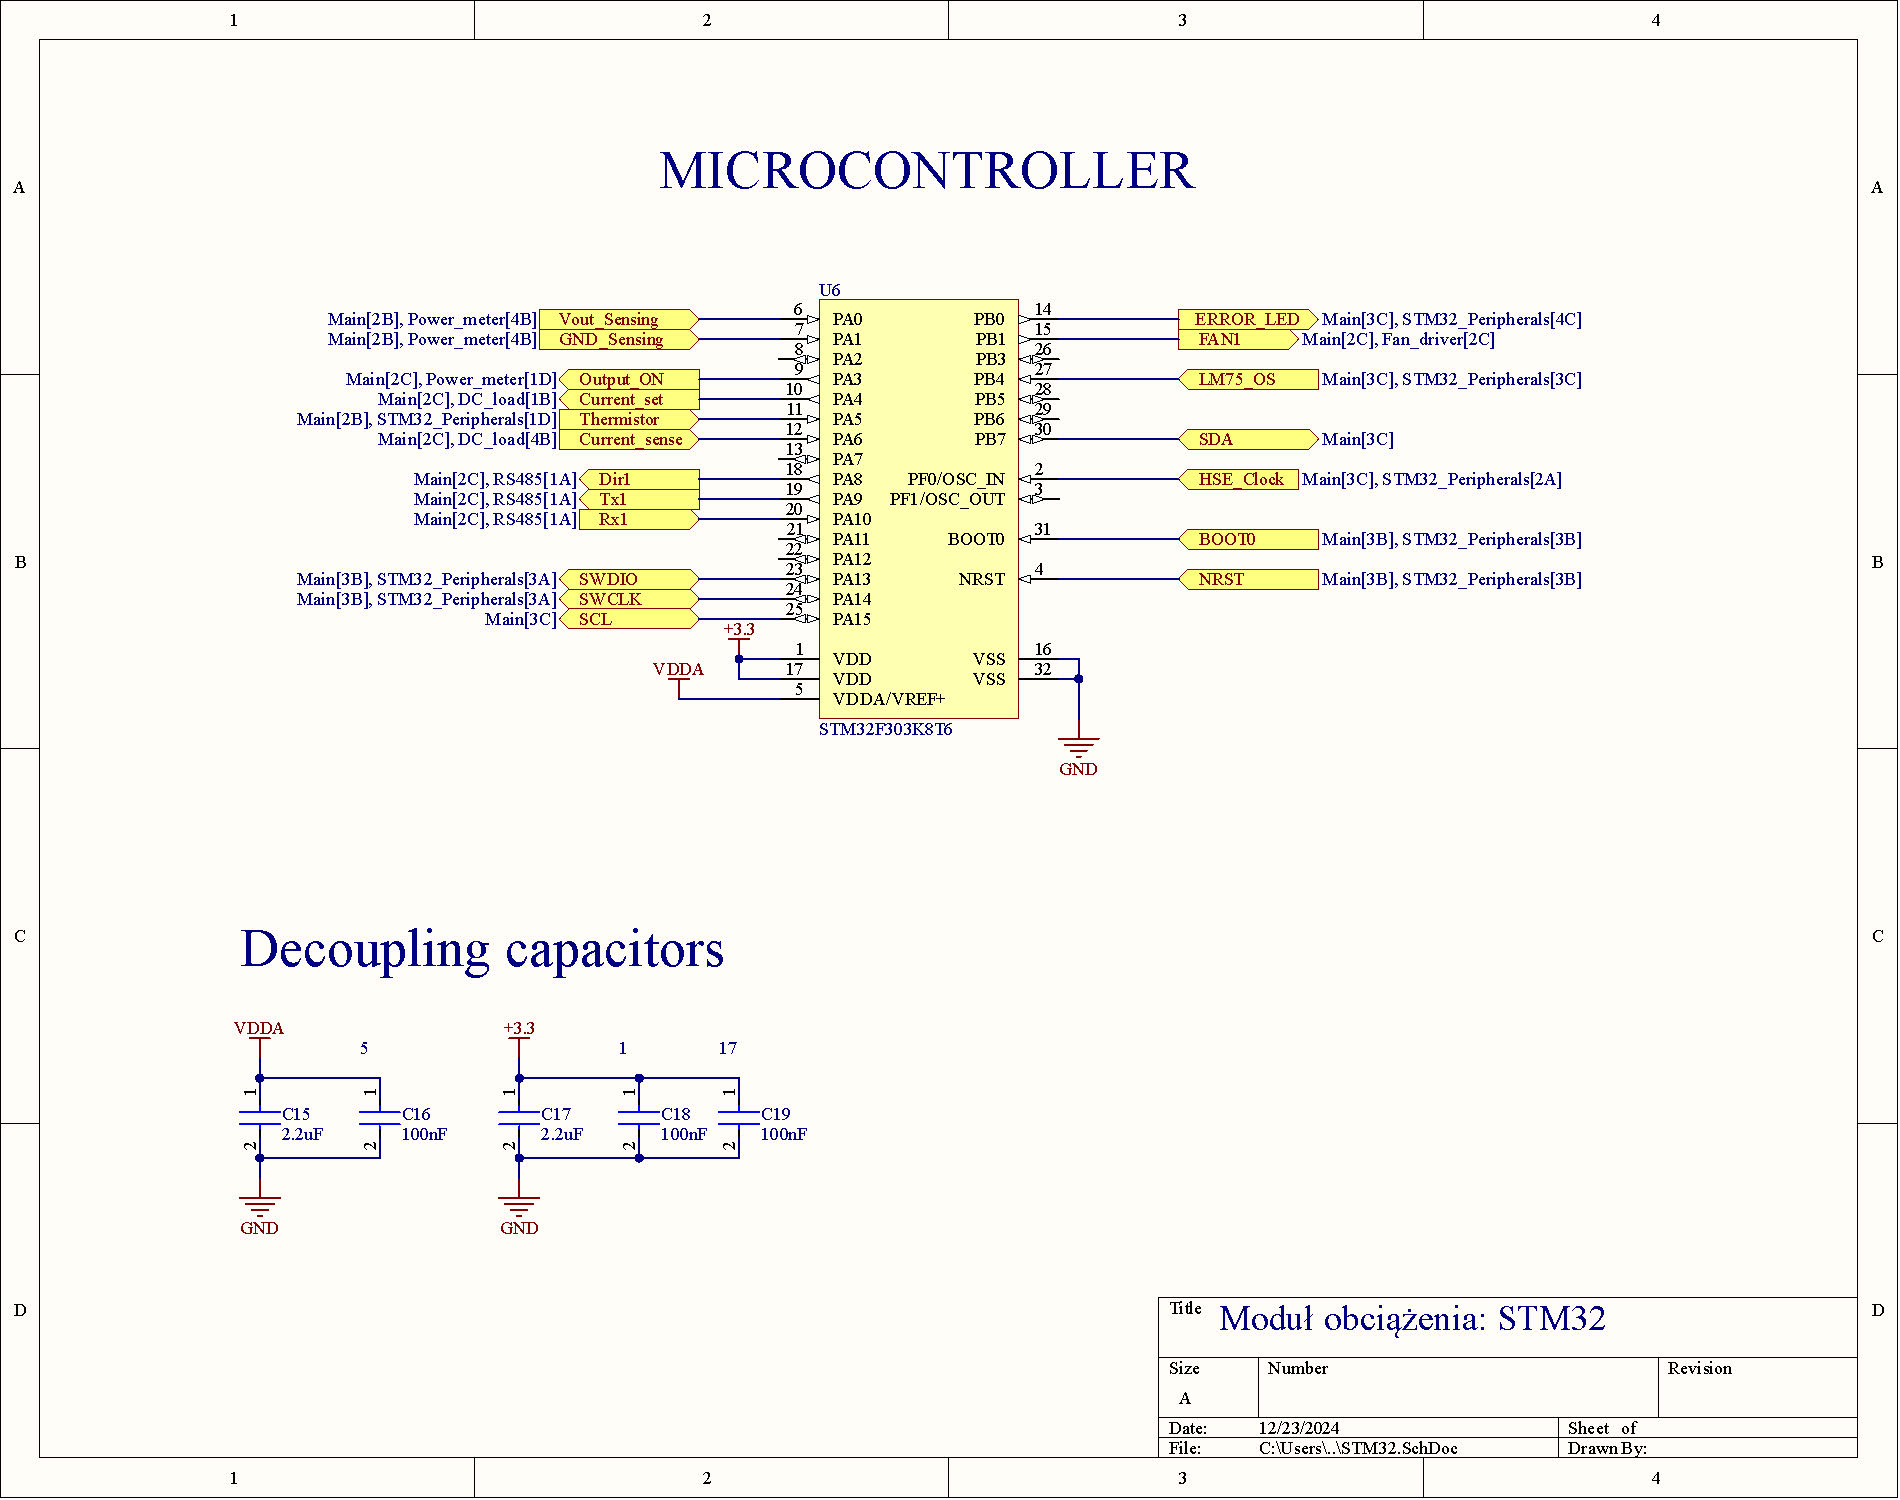
\includegraphics[width = 21cm]{zalaczniki/obciazenie/Obciążenie_aktywne_Strona_06.jpg}
        \caption{Schemat mikrokontrolera STM32.}
    \end{center}
\end{sidewaysfigure}

\begin{sidewaysfigure}
    \begin{center}
        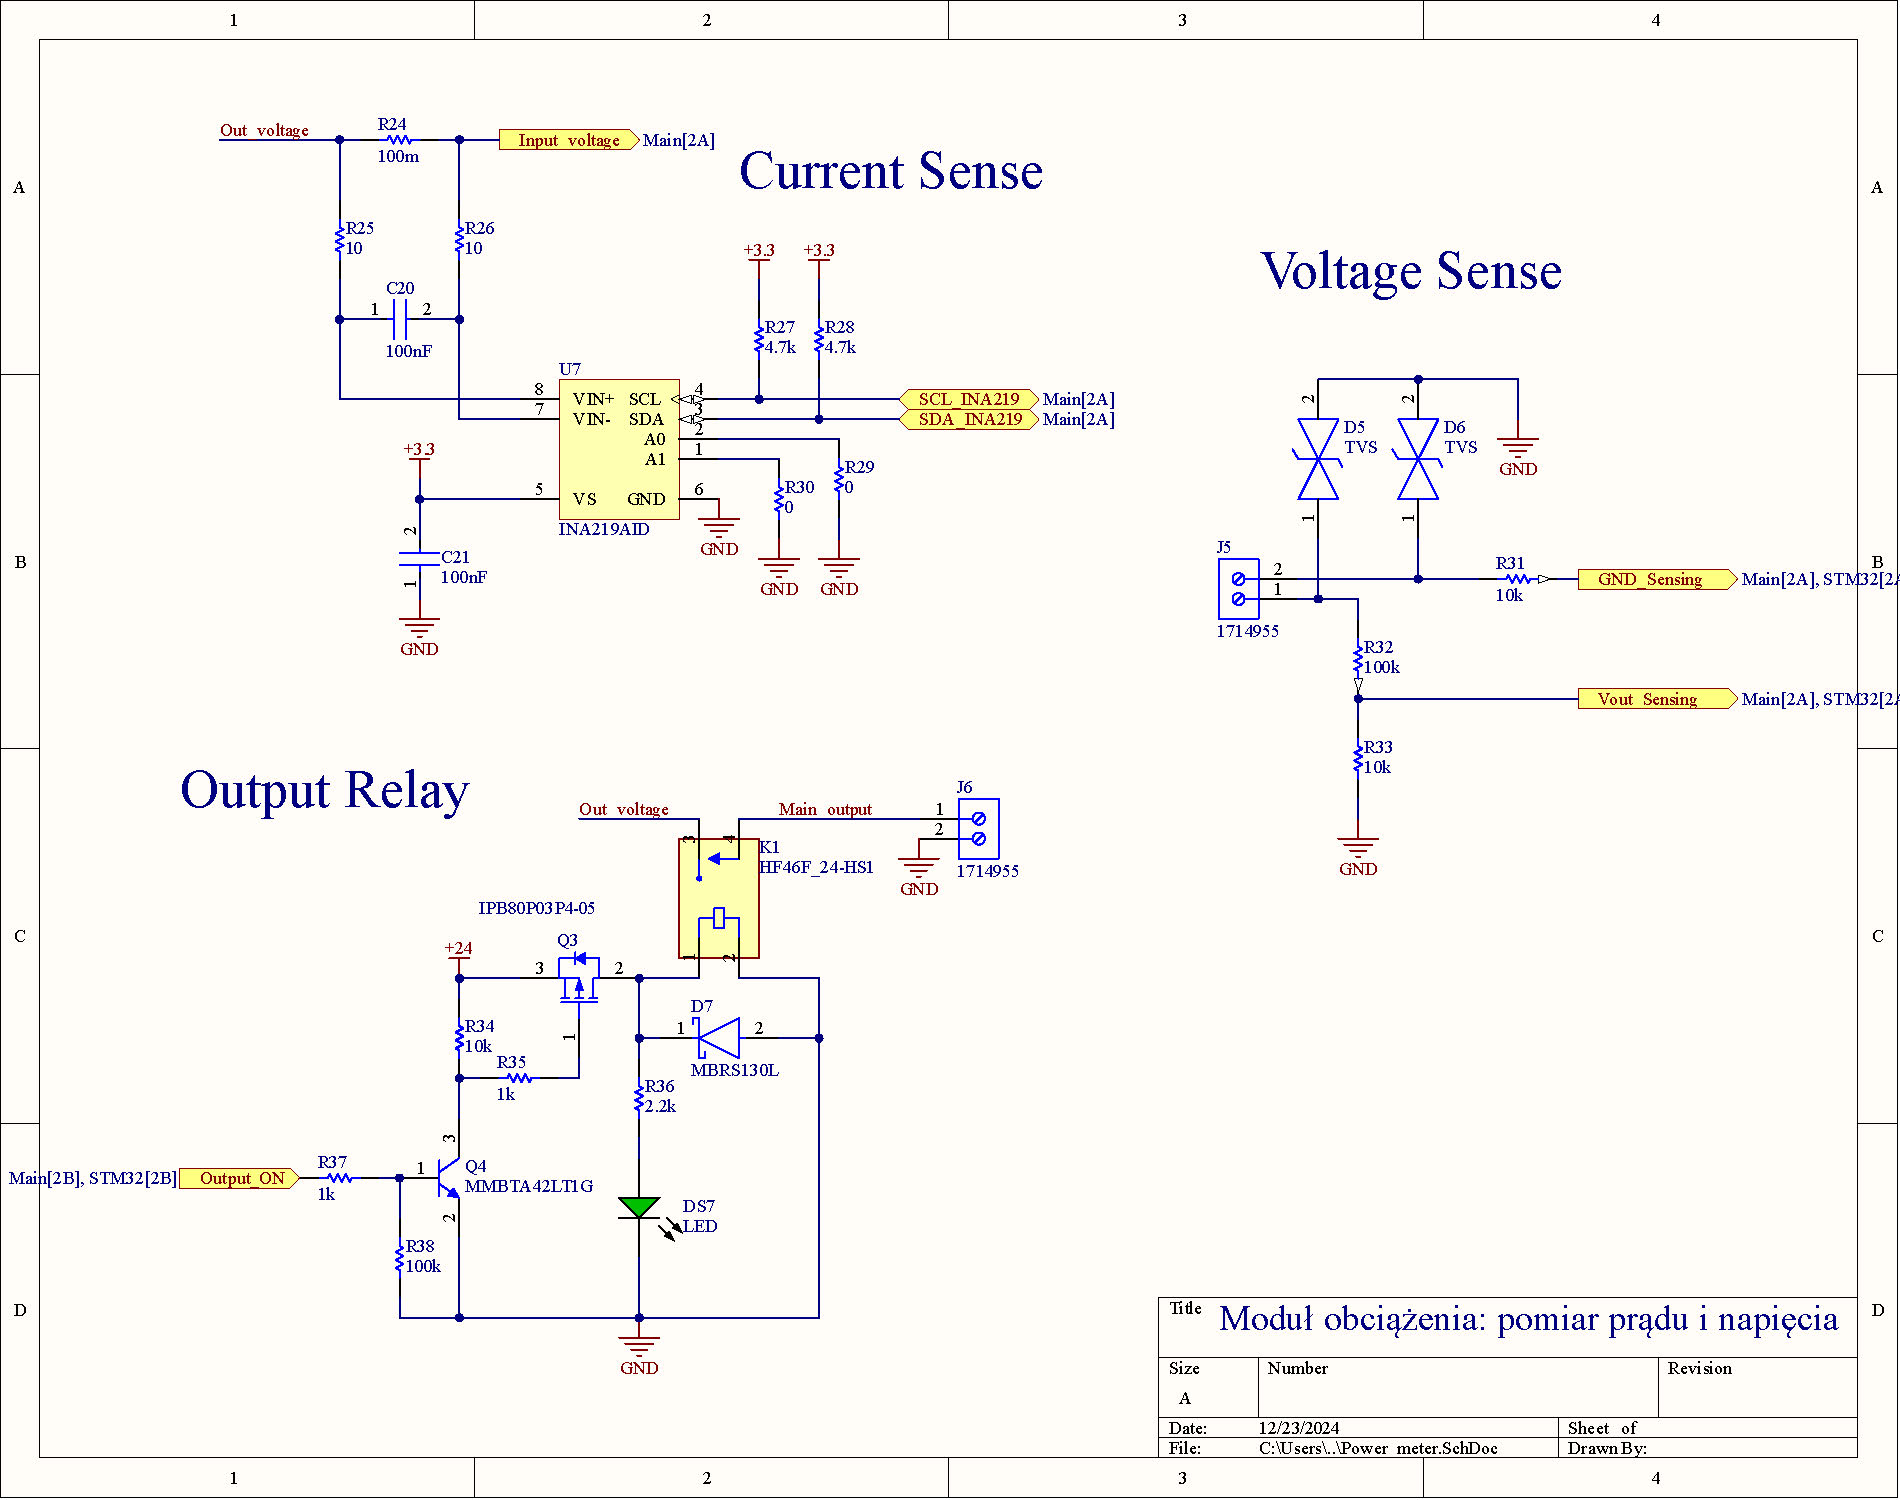
\includegraphics[width = 21cm]{zalaczniki/obciazenie/Obciążenie_aktywne_Strona_07.jpg}
        \caption{Schemat układu pomiaru prądu.}
    \end{center}
\end{sidewaysfigure}

\begin{sidewaysfigure}
    \begin{center}
        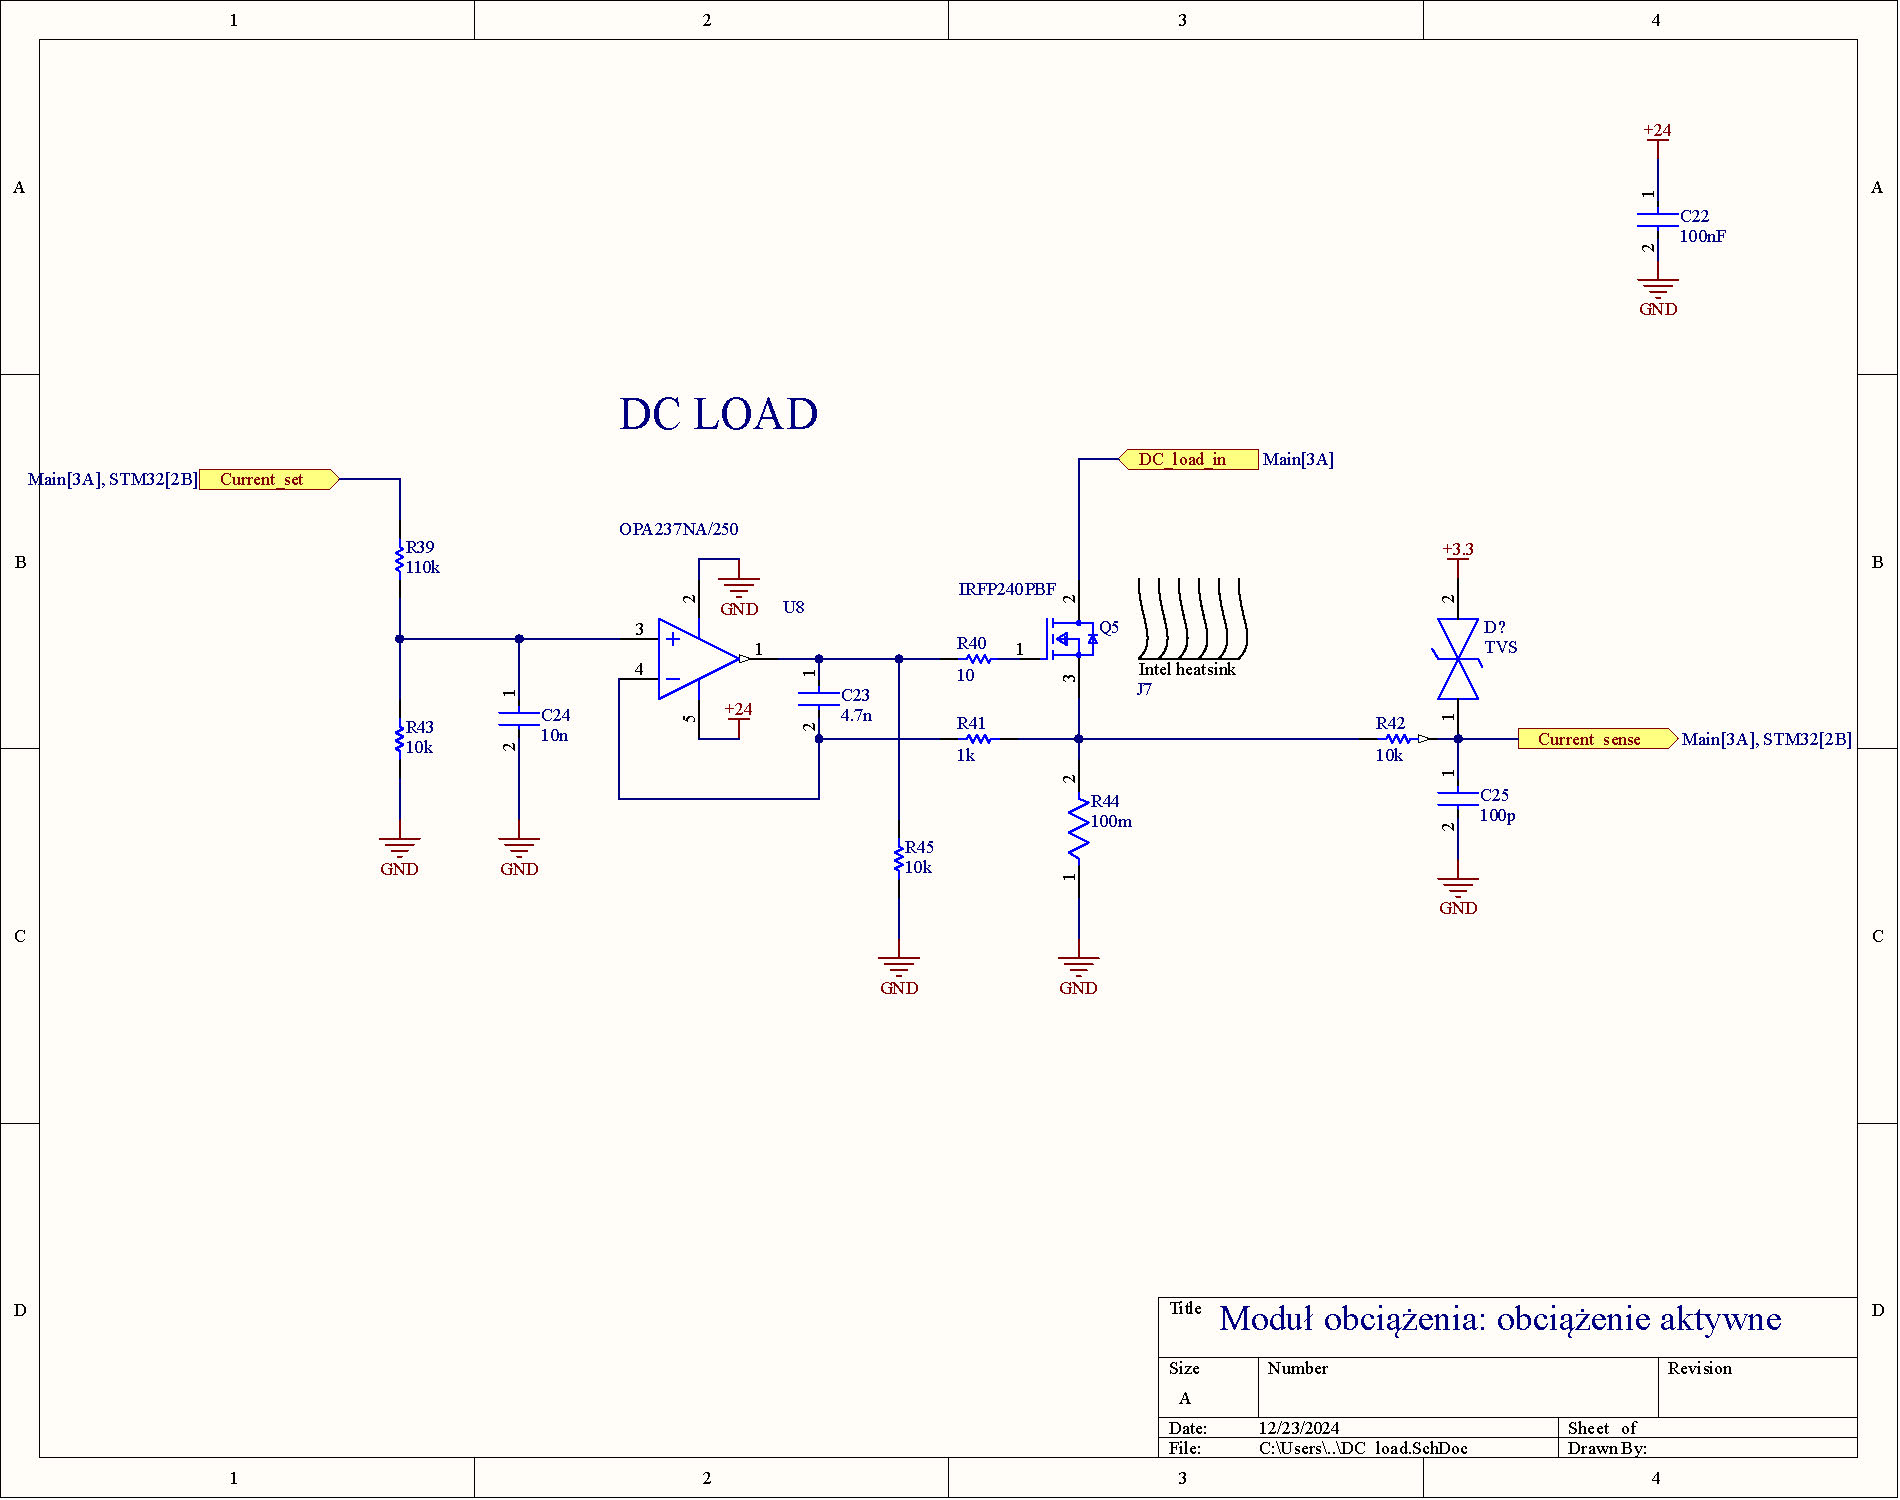
\includegraphics[width = 21cm]{zalaczniki/obciazenie/Obciążenie_aktywne_Strona_08.jpg}
        \caption{Schemat obciążenia aktywnego.}
    \end{center}
\end{sidewaysfigure}

\begin{figure}
    \begin{center}
        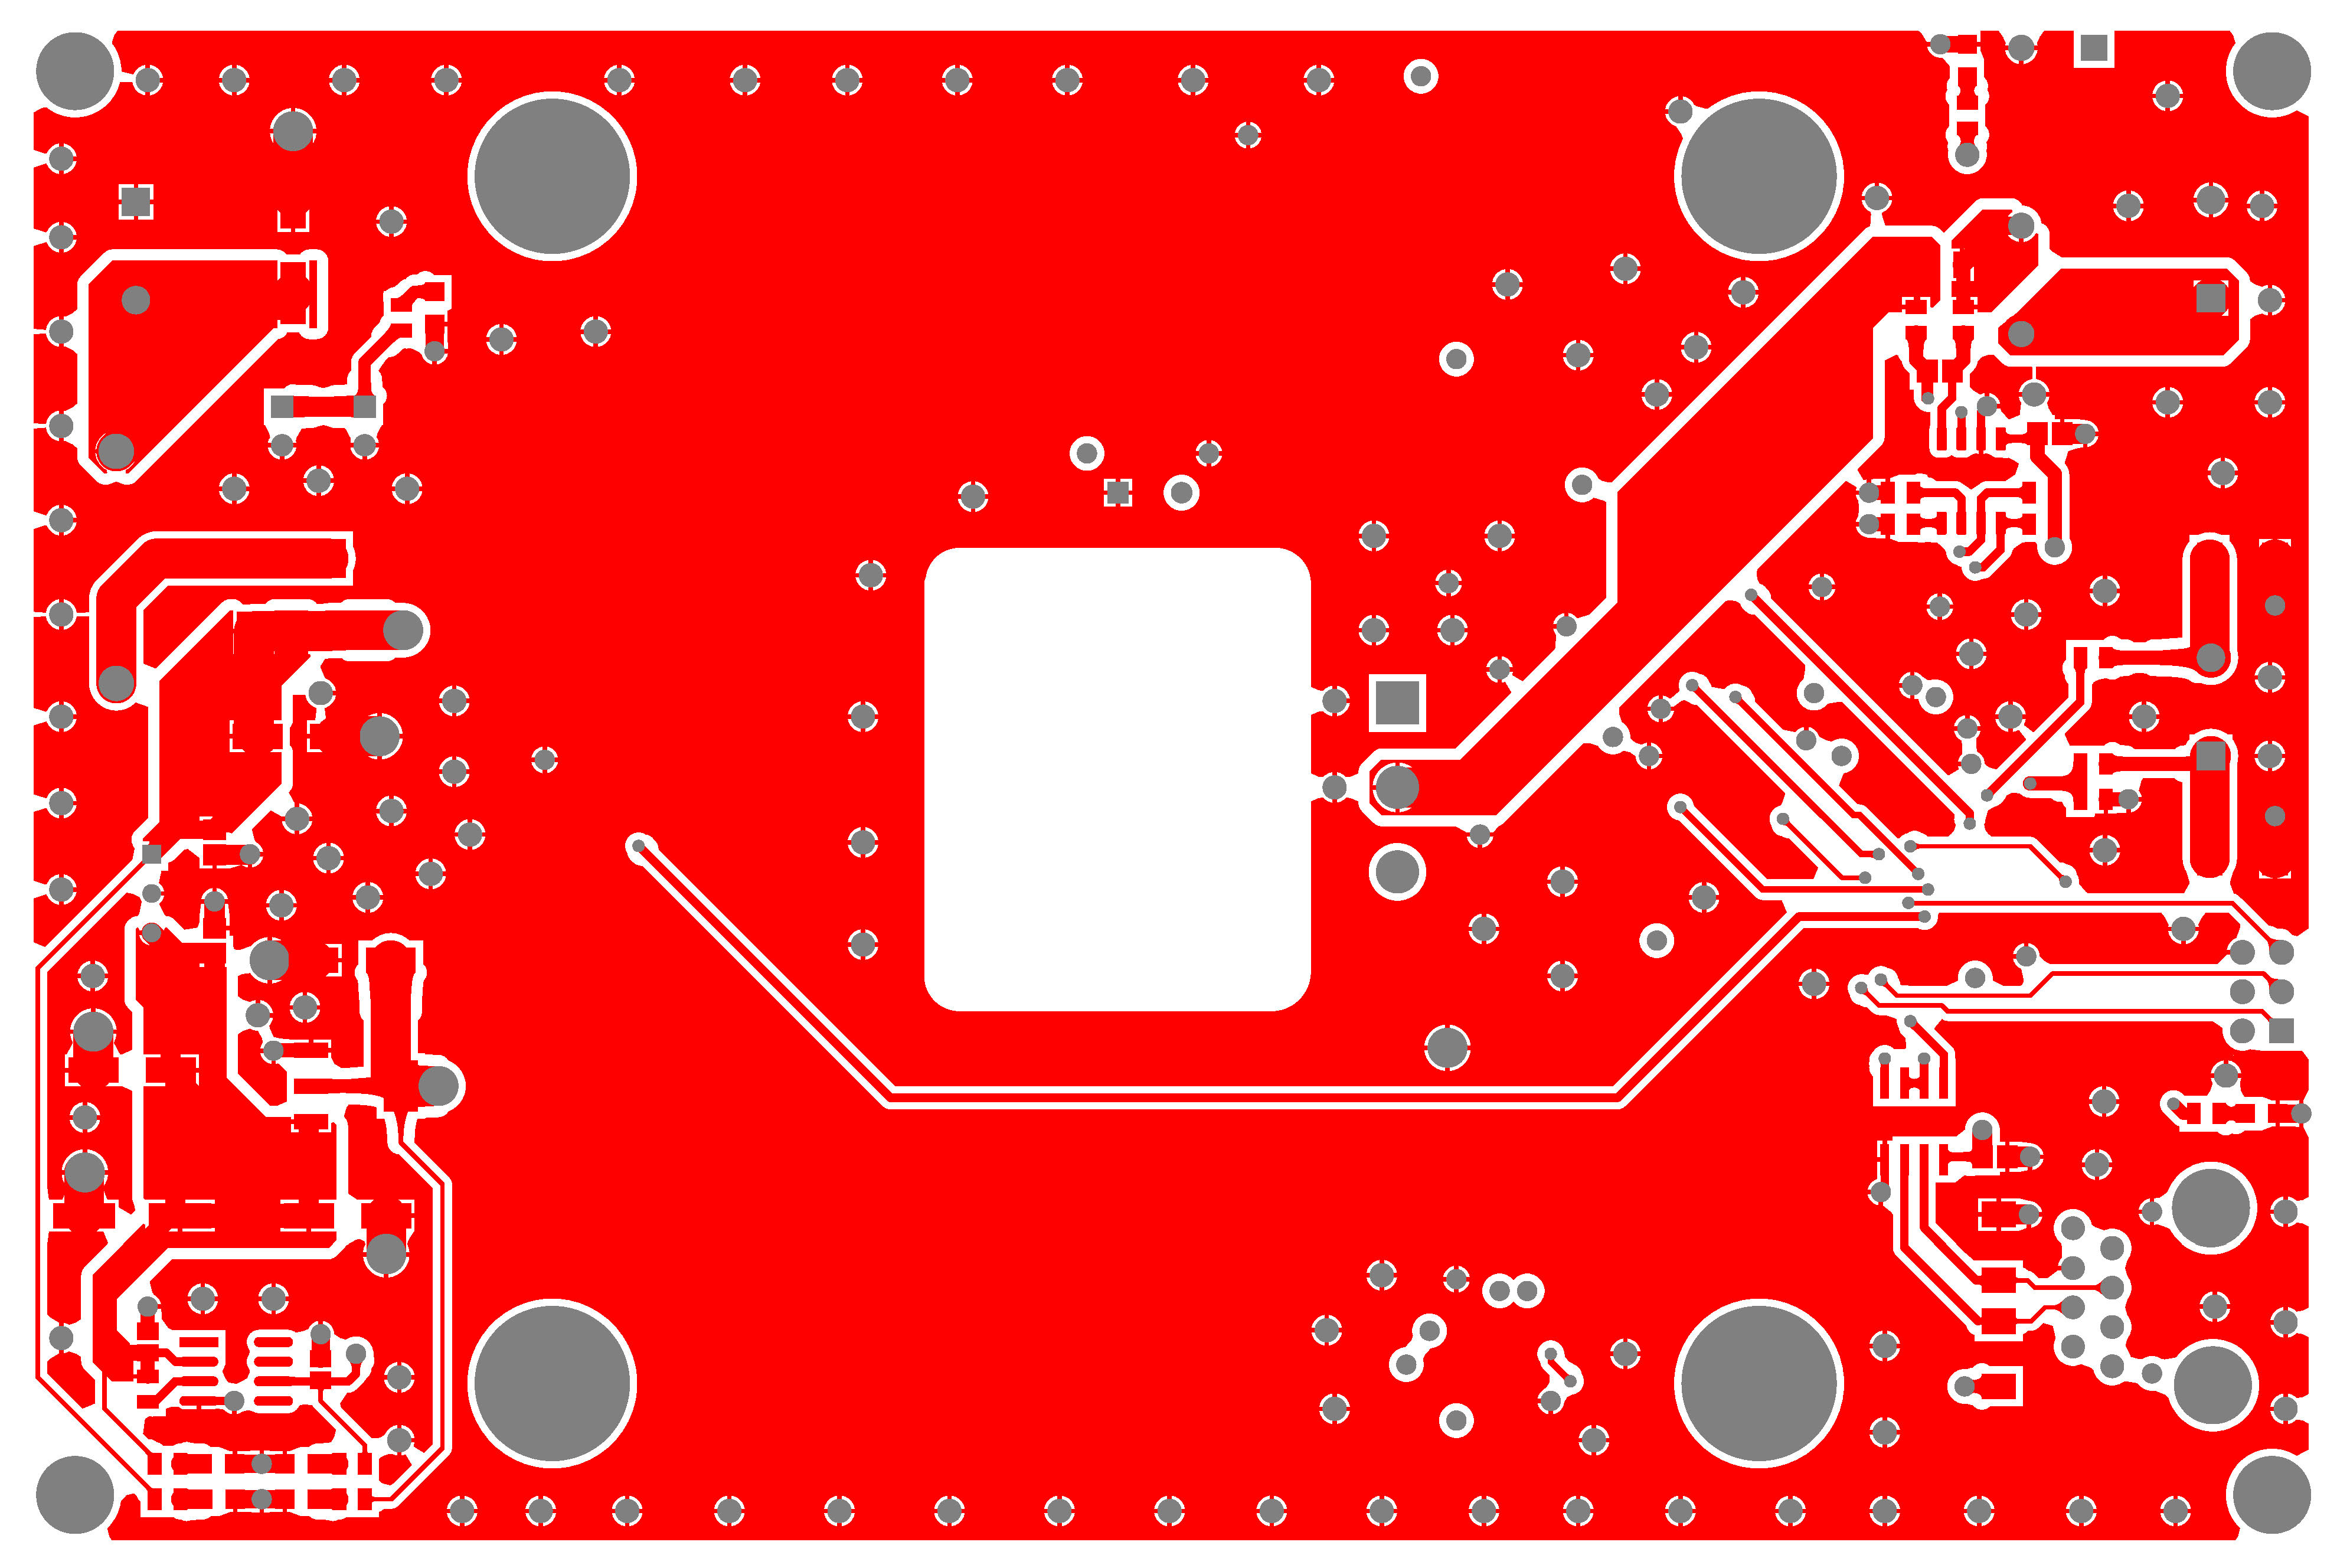
\includegraphics[width = 15cm]{zalaczniki/obciazenie/Obciążenie_aktywne_Strona_09.jpg}
        \caption{Warstwa górna PCB.}
    \end{center}
\end{figure}

\begin{figure}
    \begin{center}
        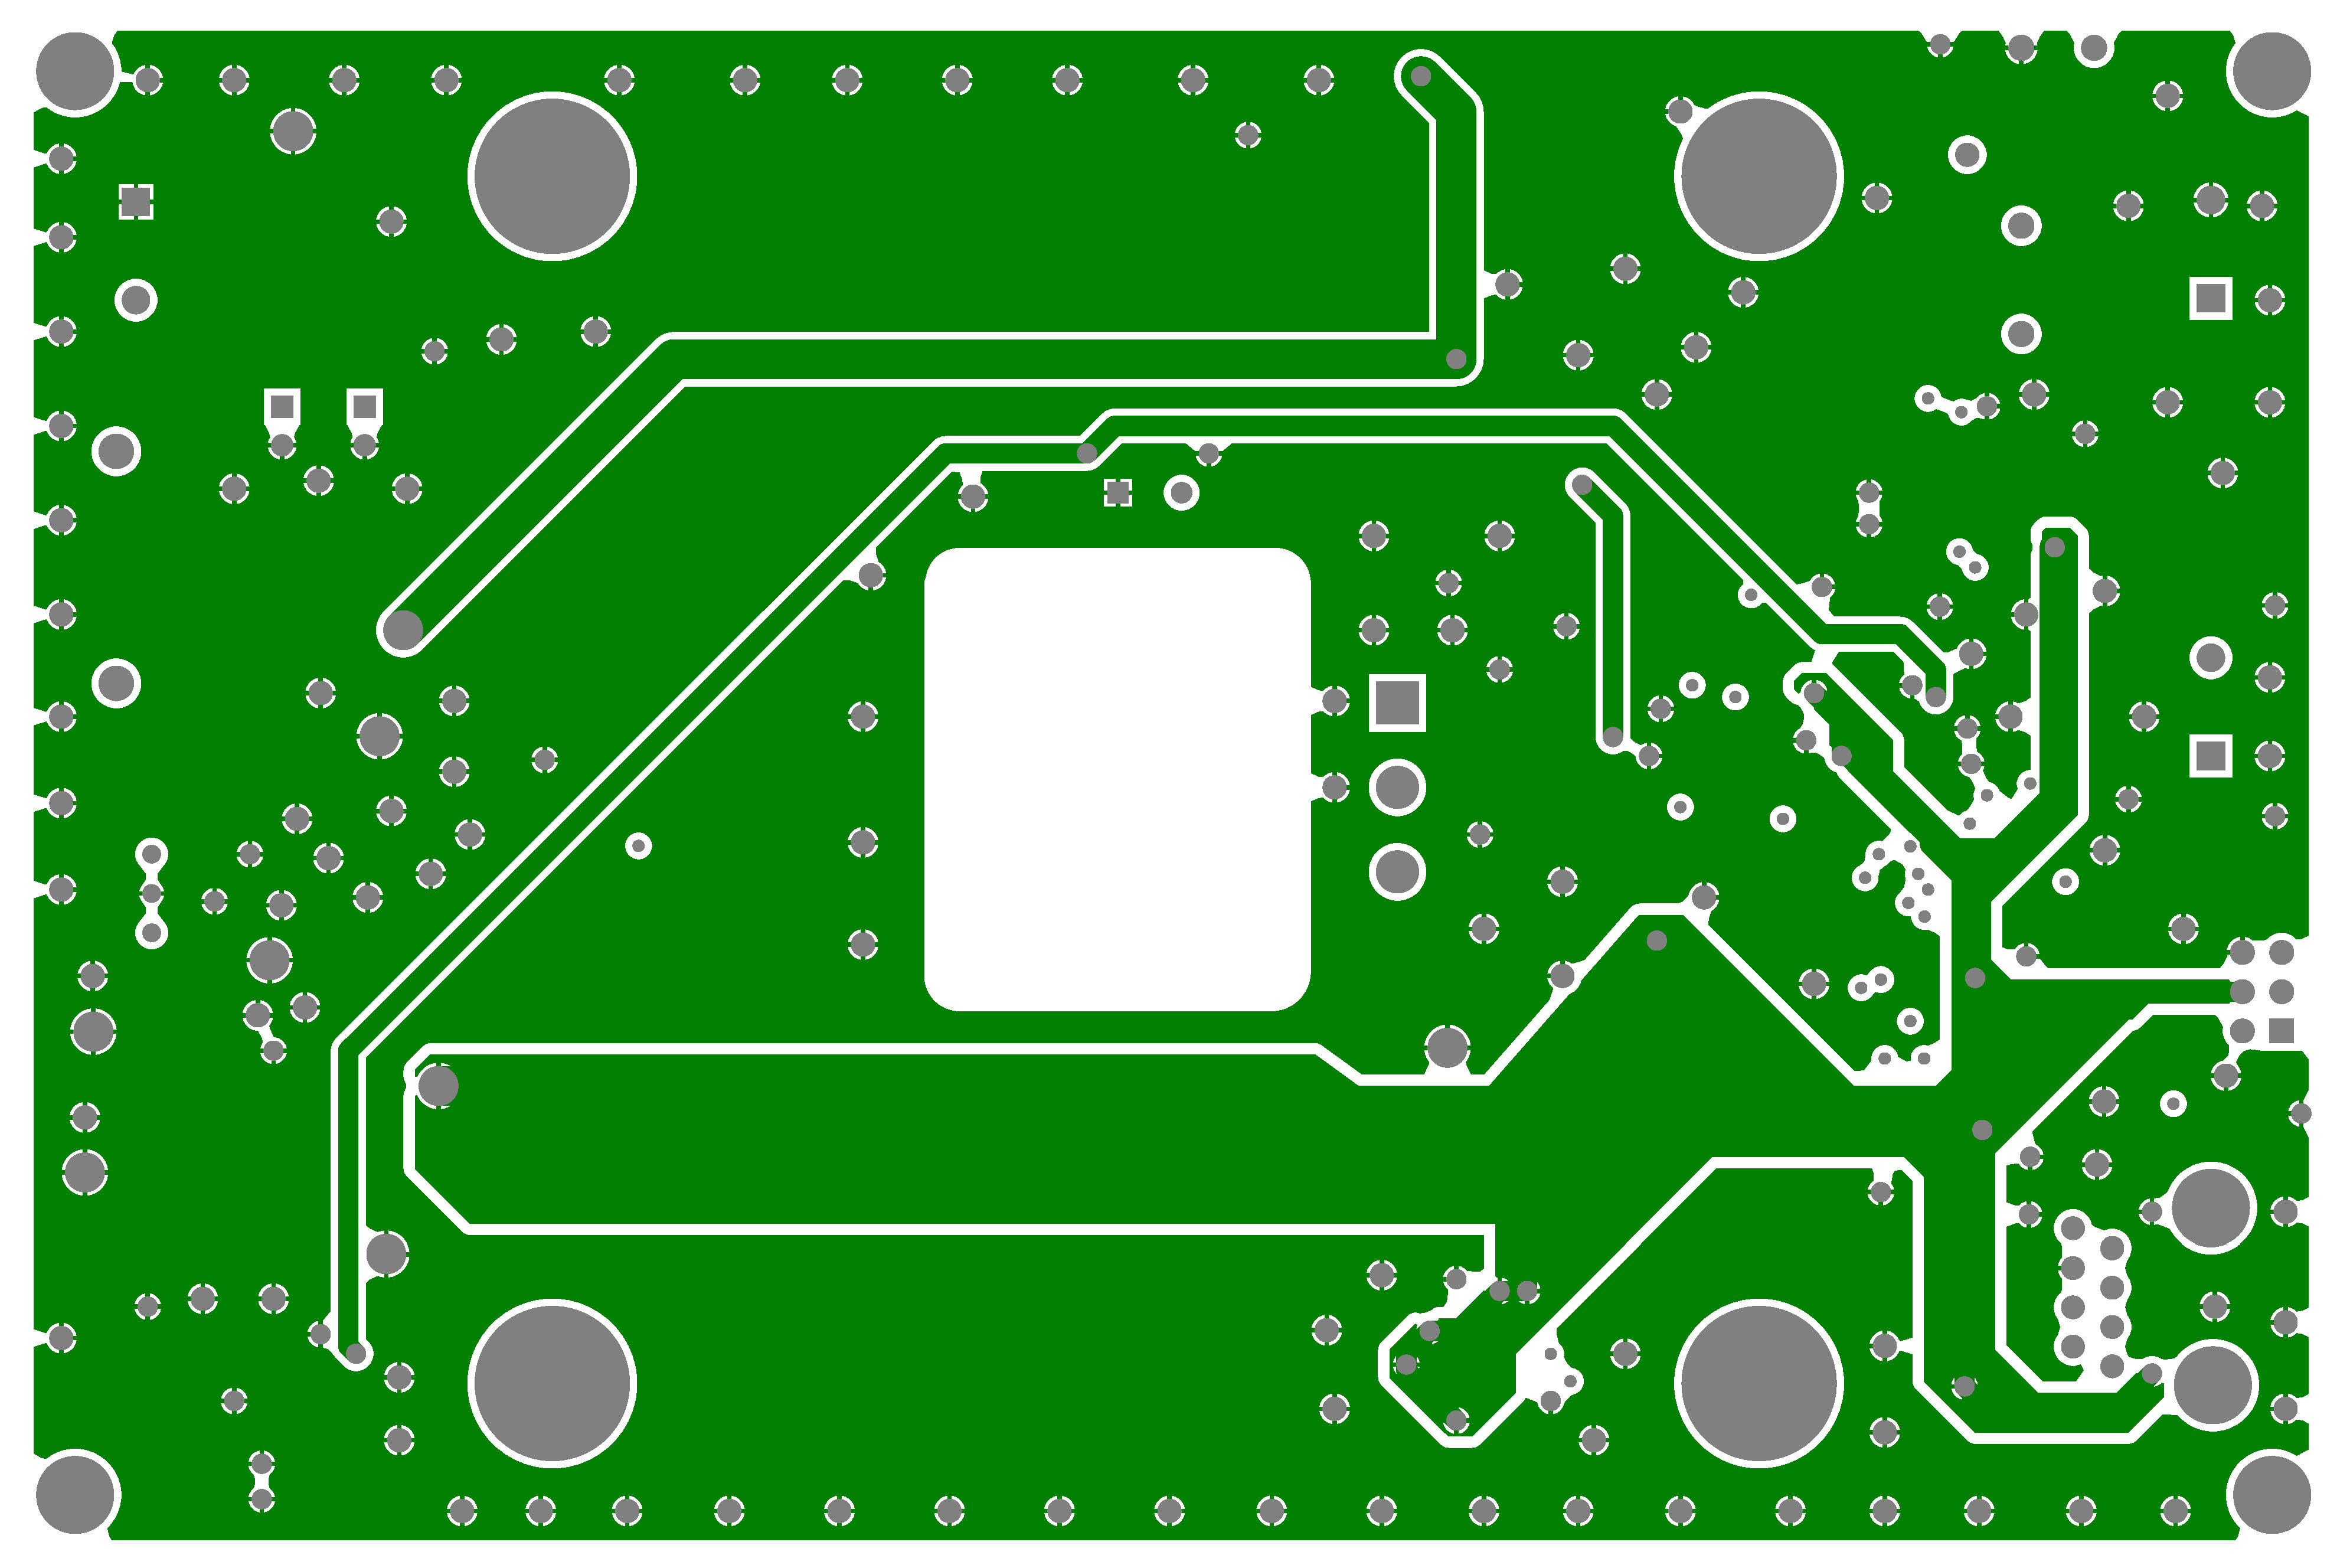
\includegraphics[width = 15cm]{zalaczniki/obciazenie/Obciążenie_aktywne_Strona_10.jpg}
        \caption{Warstwa wewnętrzna 2 PCB.}
    \end{center}
\end{figure}

\begin{figure}
    \begin{center}
        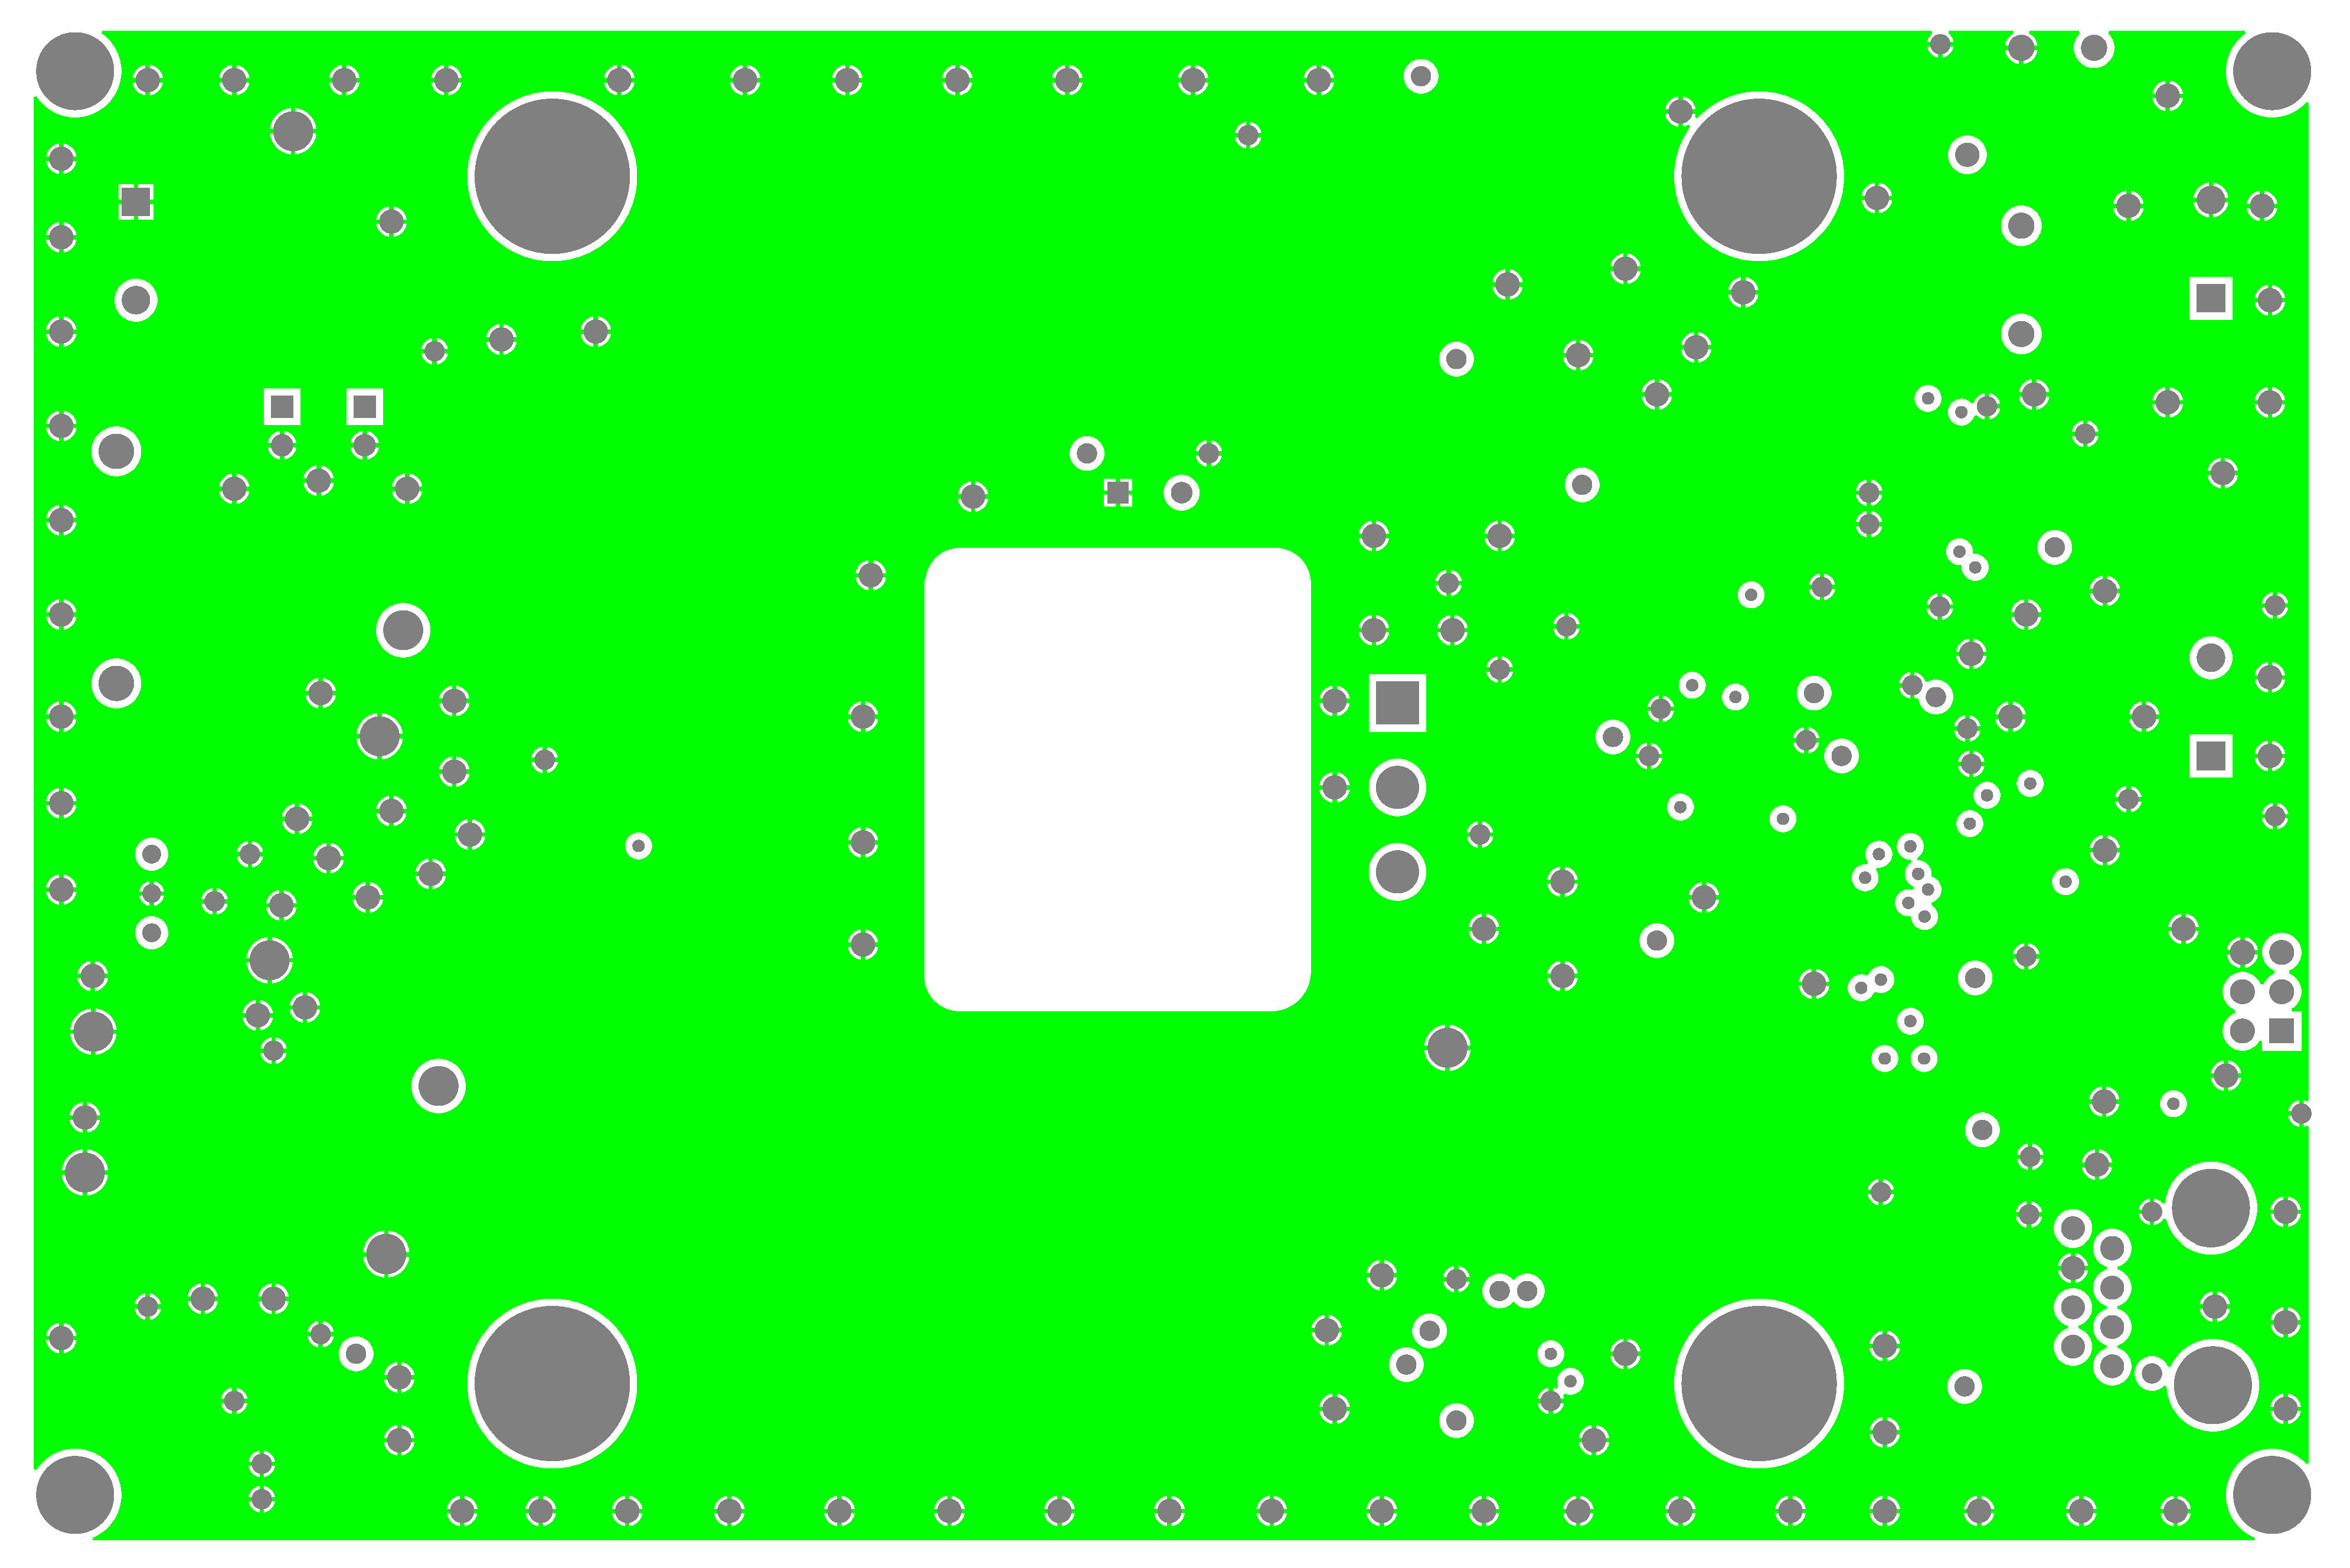
\includegraphics[width = 15cm]{zalaczniki/obciazenie/Obciążenie_aktywne_Strona_11.jpg}
        \caption{Warstwa wewnętrzna 2 PCB.}
    \end{center}
\end{figure}

\begin{figure}
    \begin{center}
        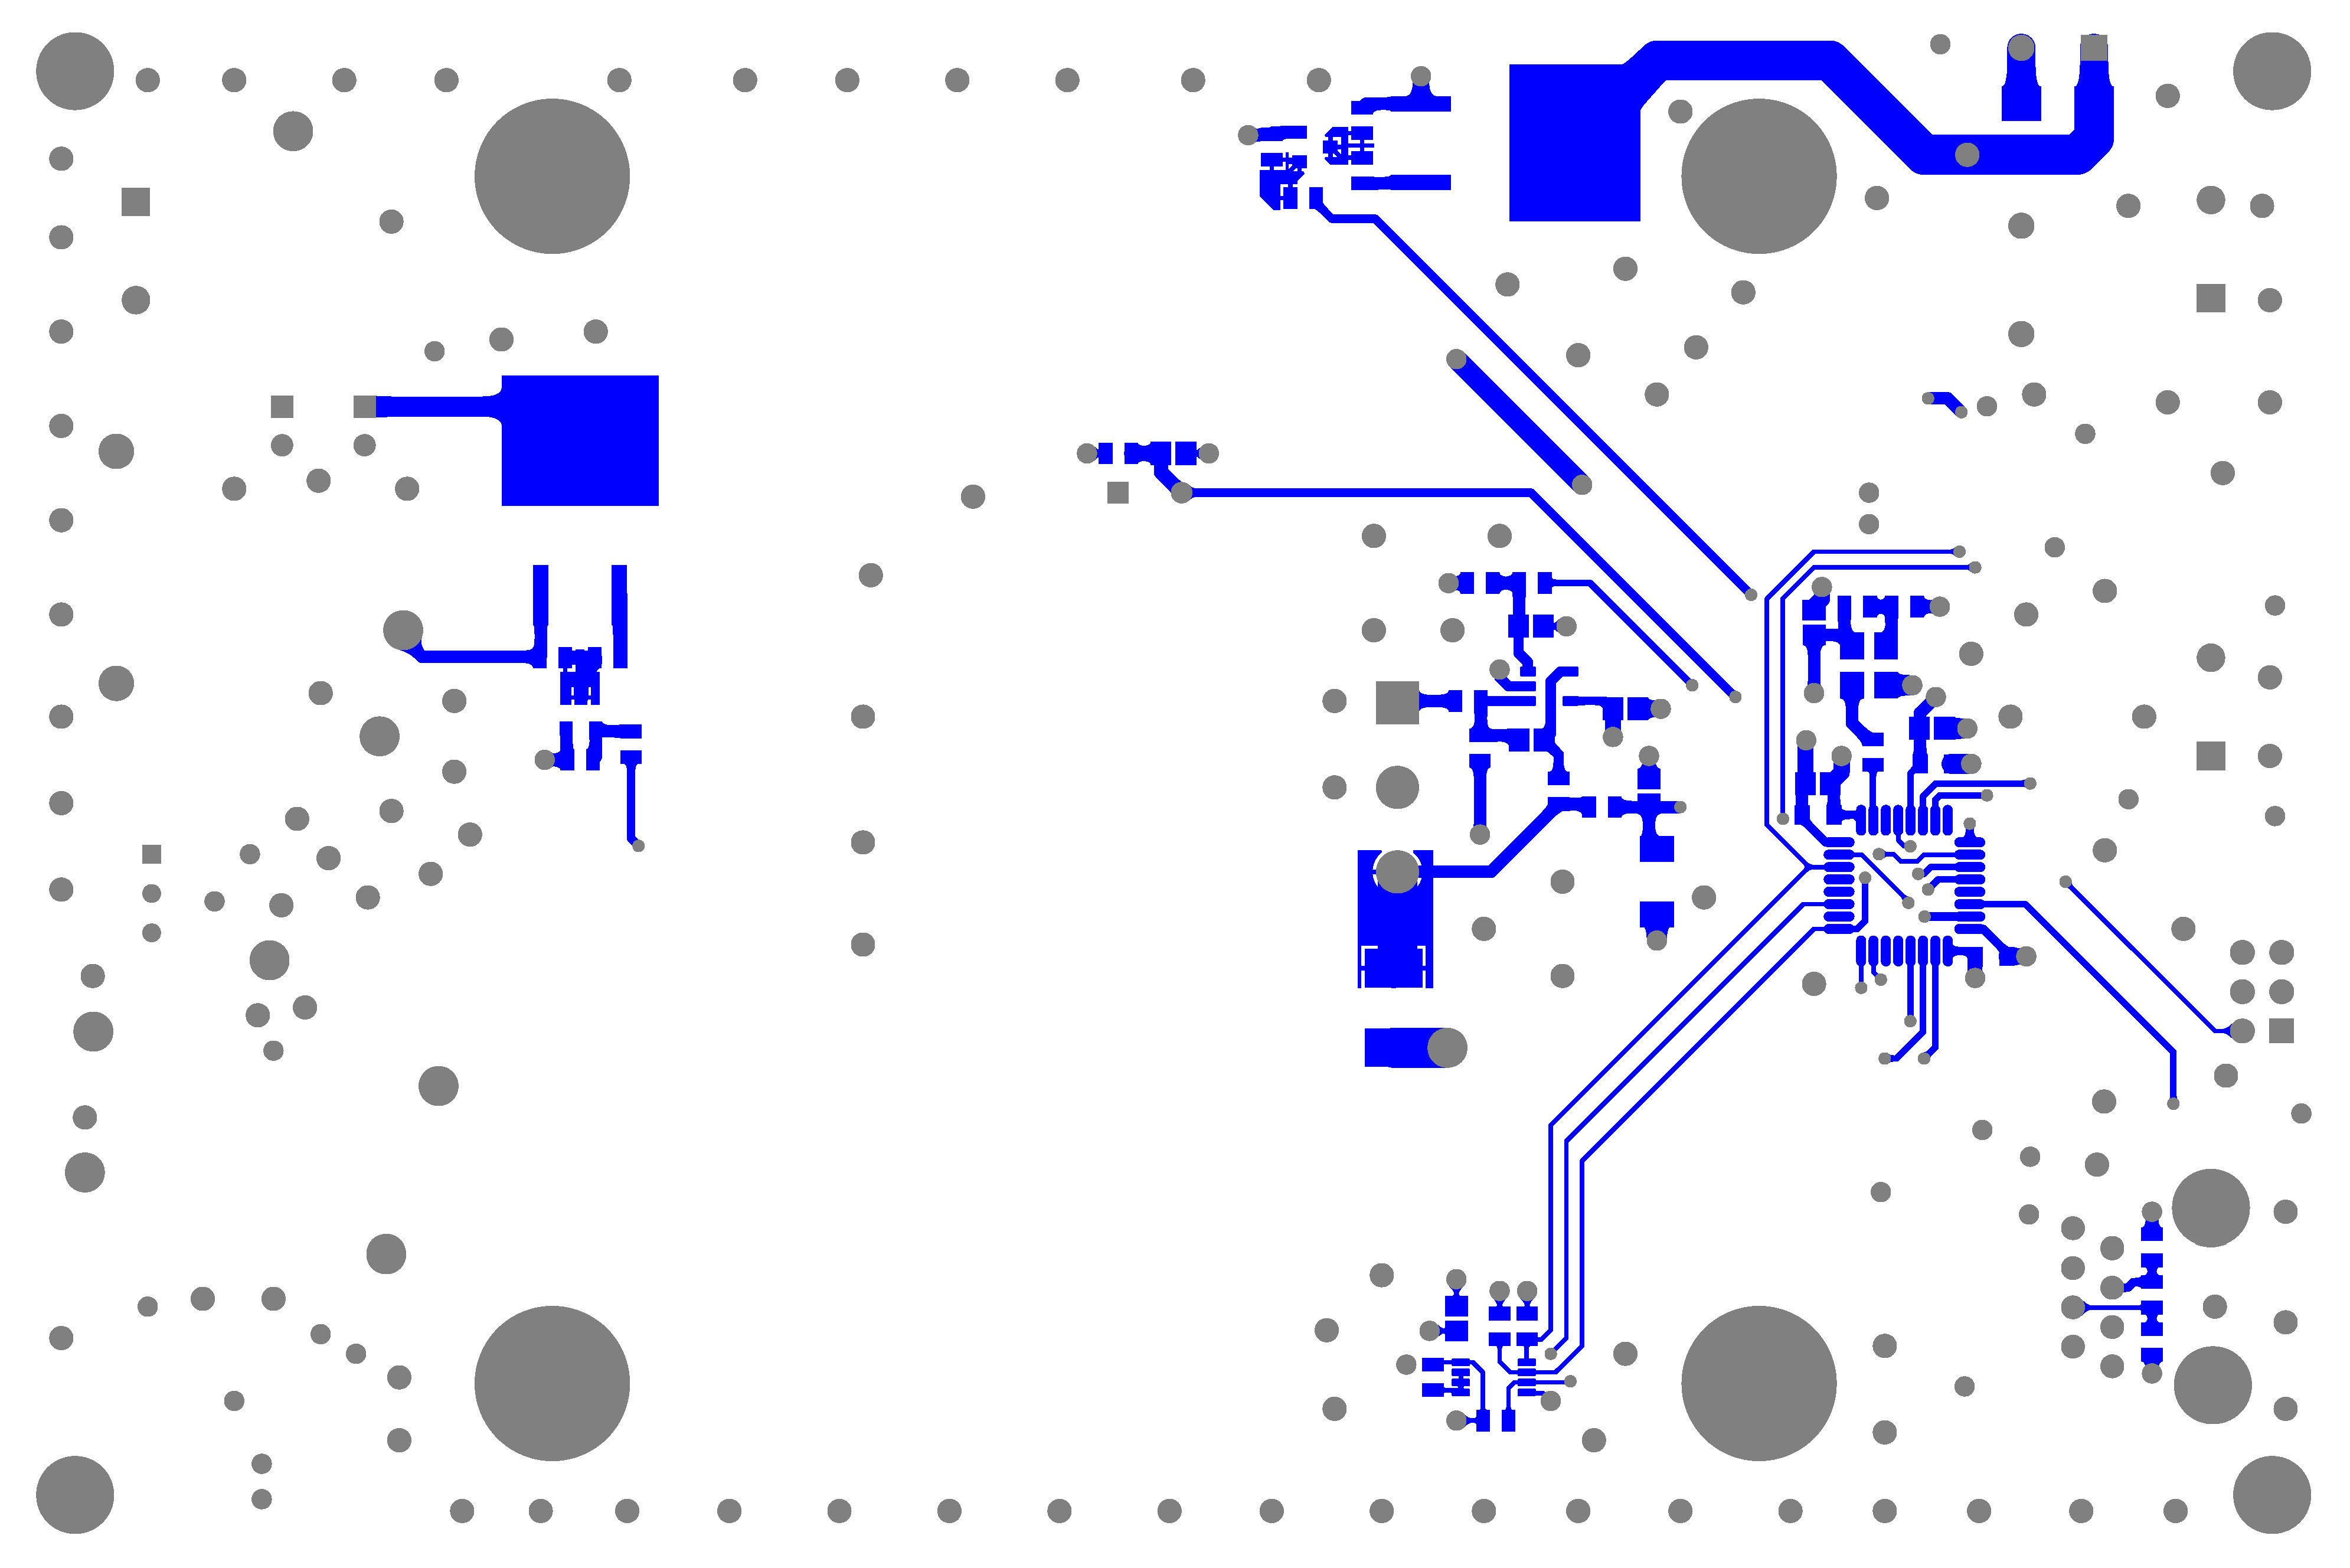
\includegraphics[width = 15cm]{zalaczniki/obciazenie/Obciążenie_aktywne_Strona_12.jpg}
        \caption{Warstwa dolna PCB.}
    \end{center}
\end{figure}


\nopagebreak

\chapter{Panele przycisków}


\begin{figure}[h!]%
    \centering
    \subfloat[\centering Panel lewy]{{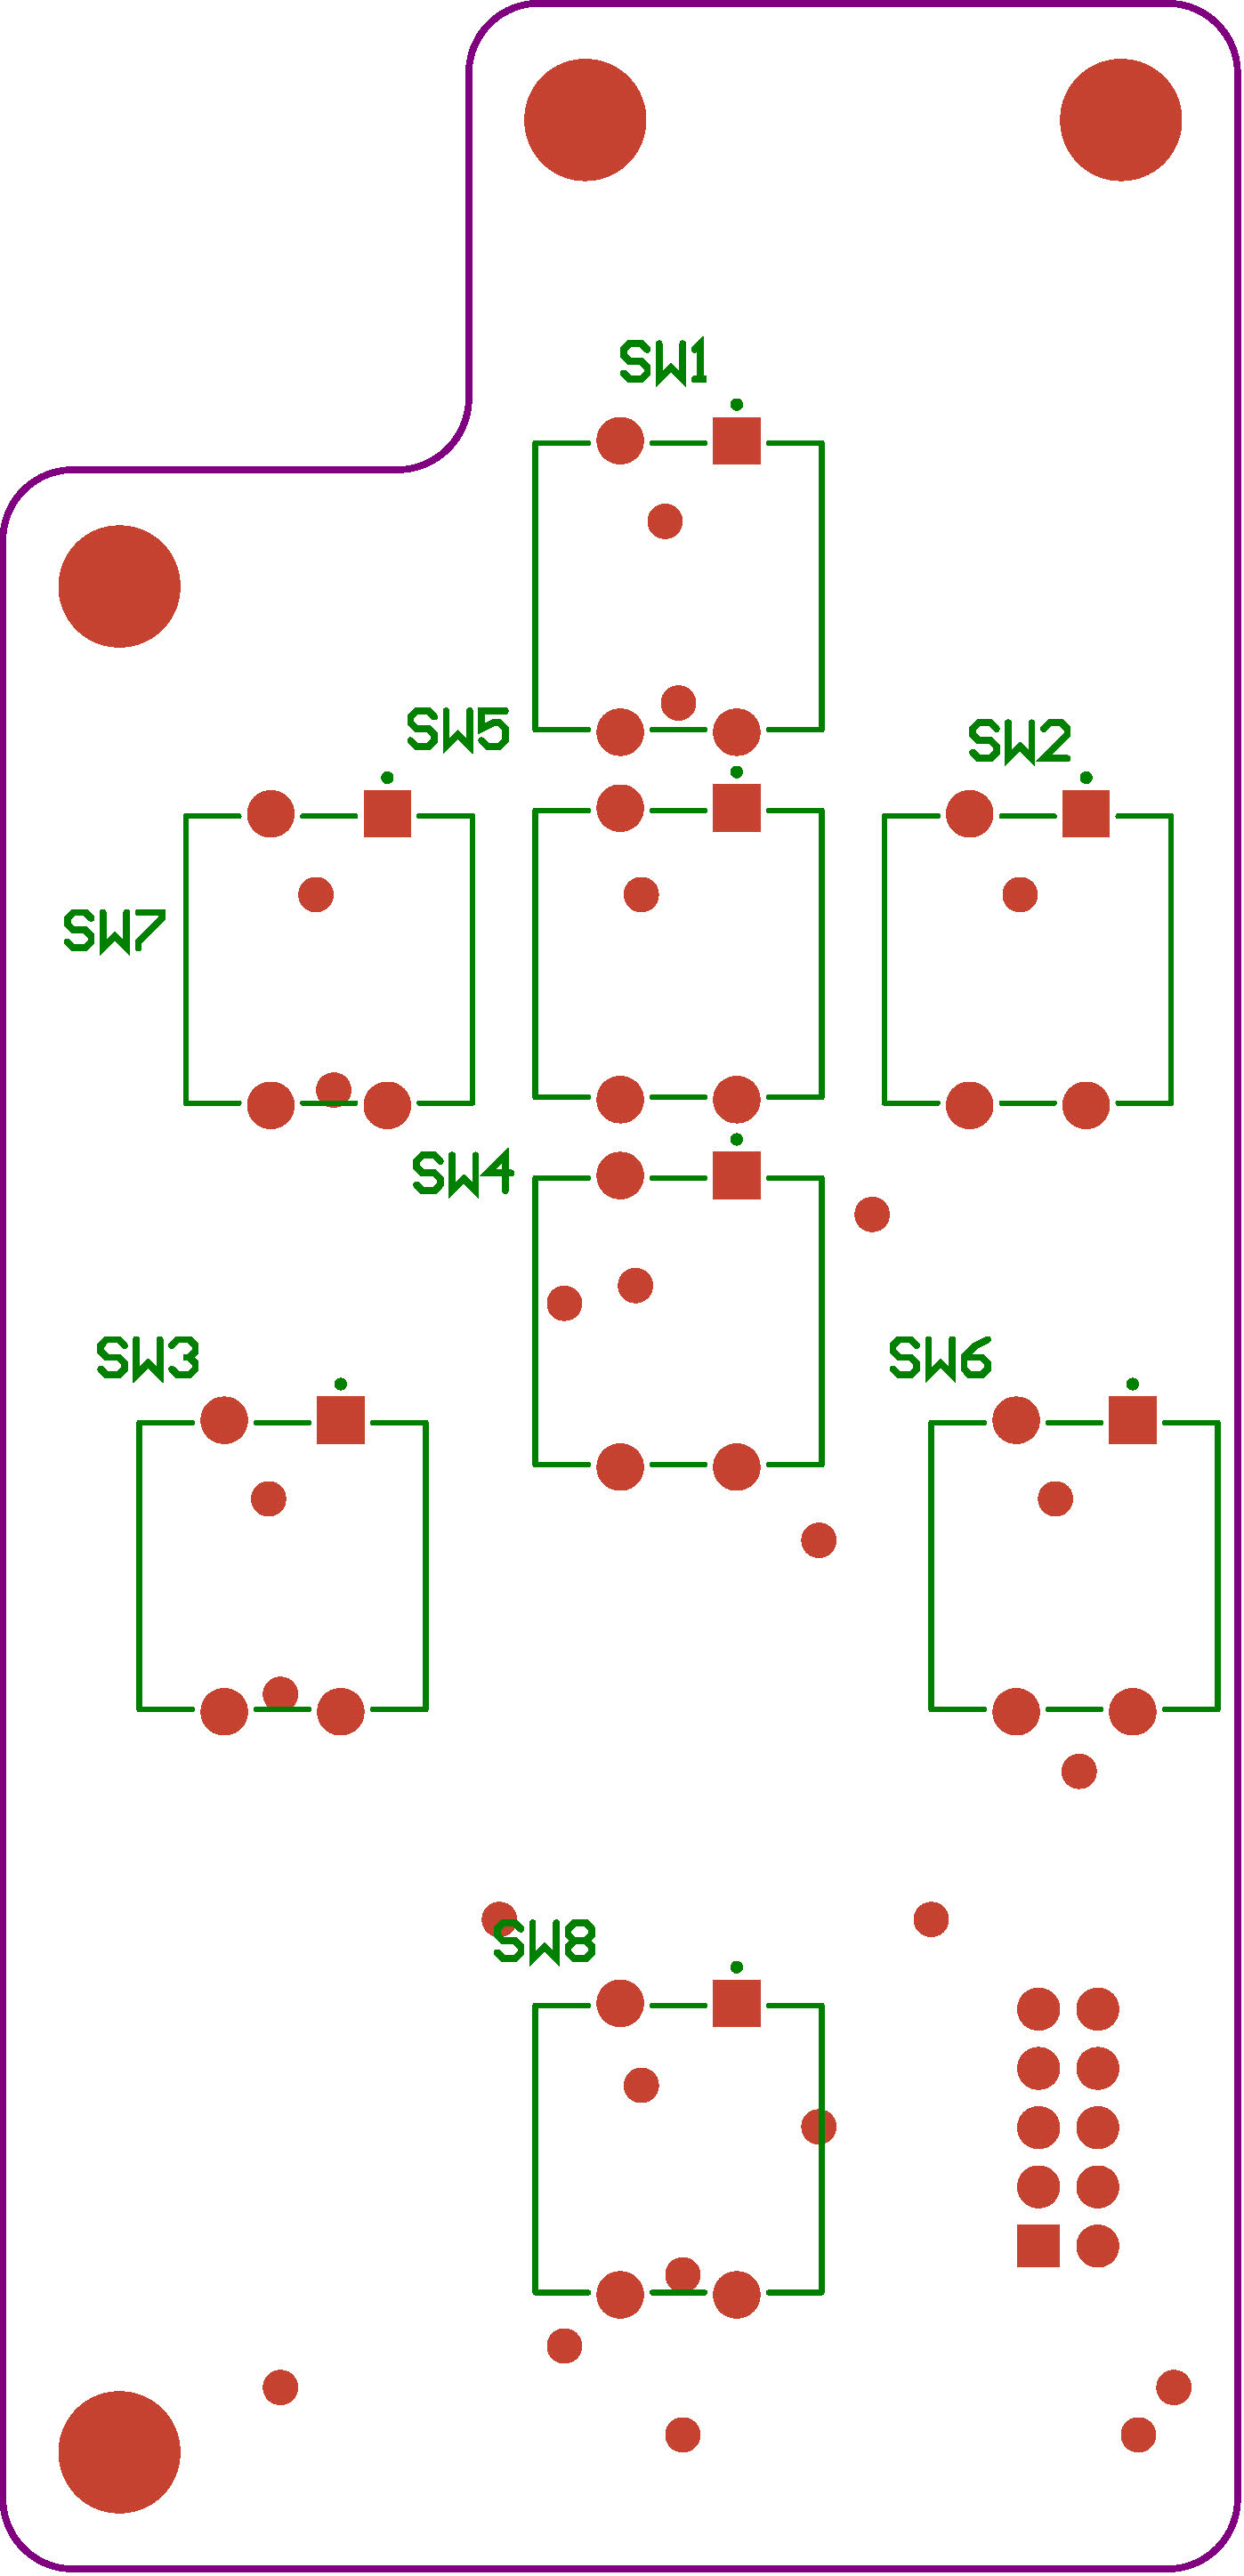
\includegraphics[width=7.5cm]{zalaczniki/przyciski/Przyciski_prawe_Strona_4.jpg} }}%
    \qquad
    \subfloat[\centering Panel prawy.]{{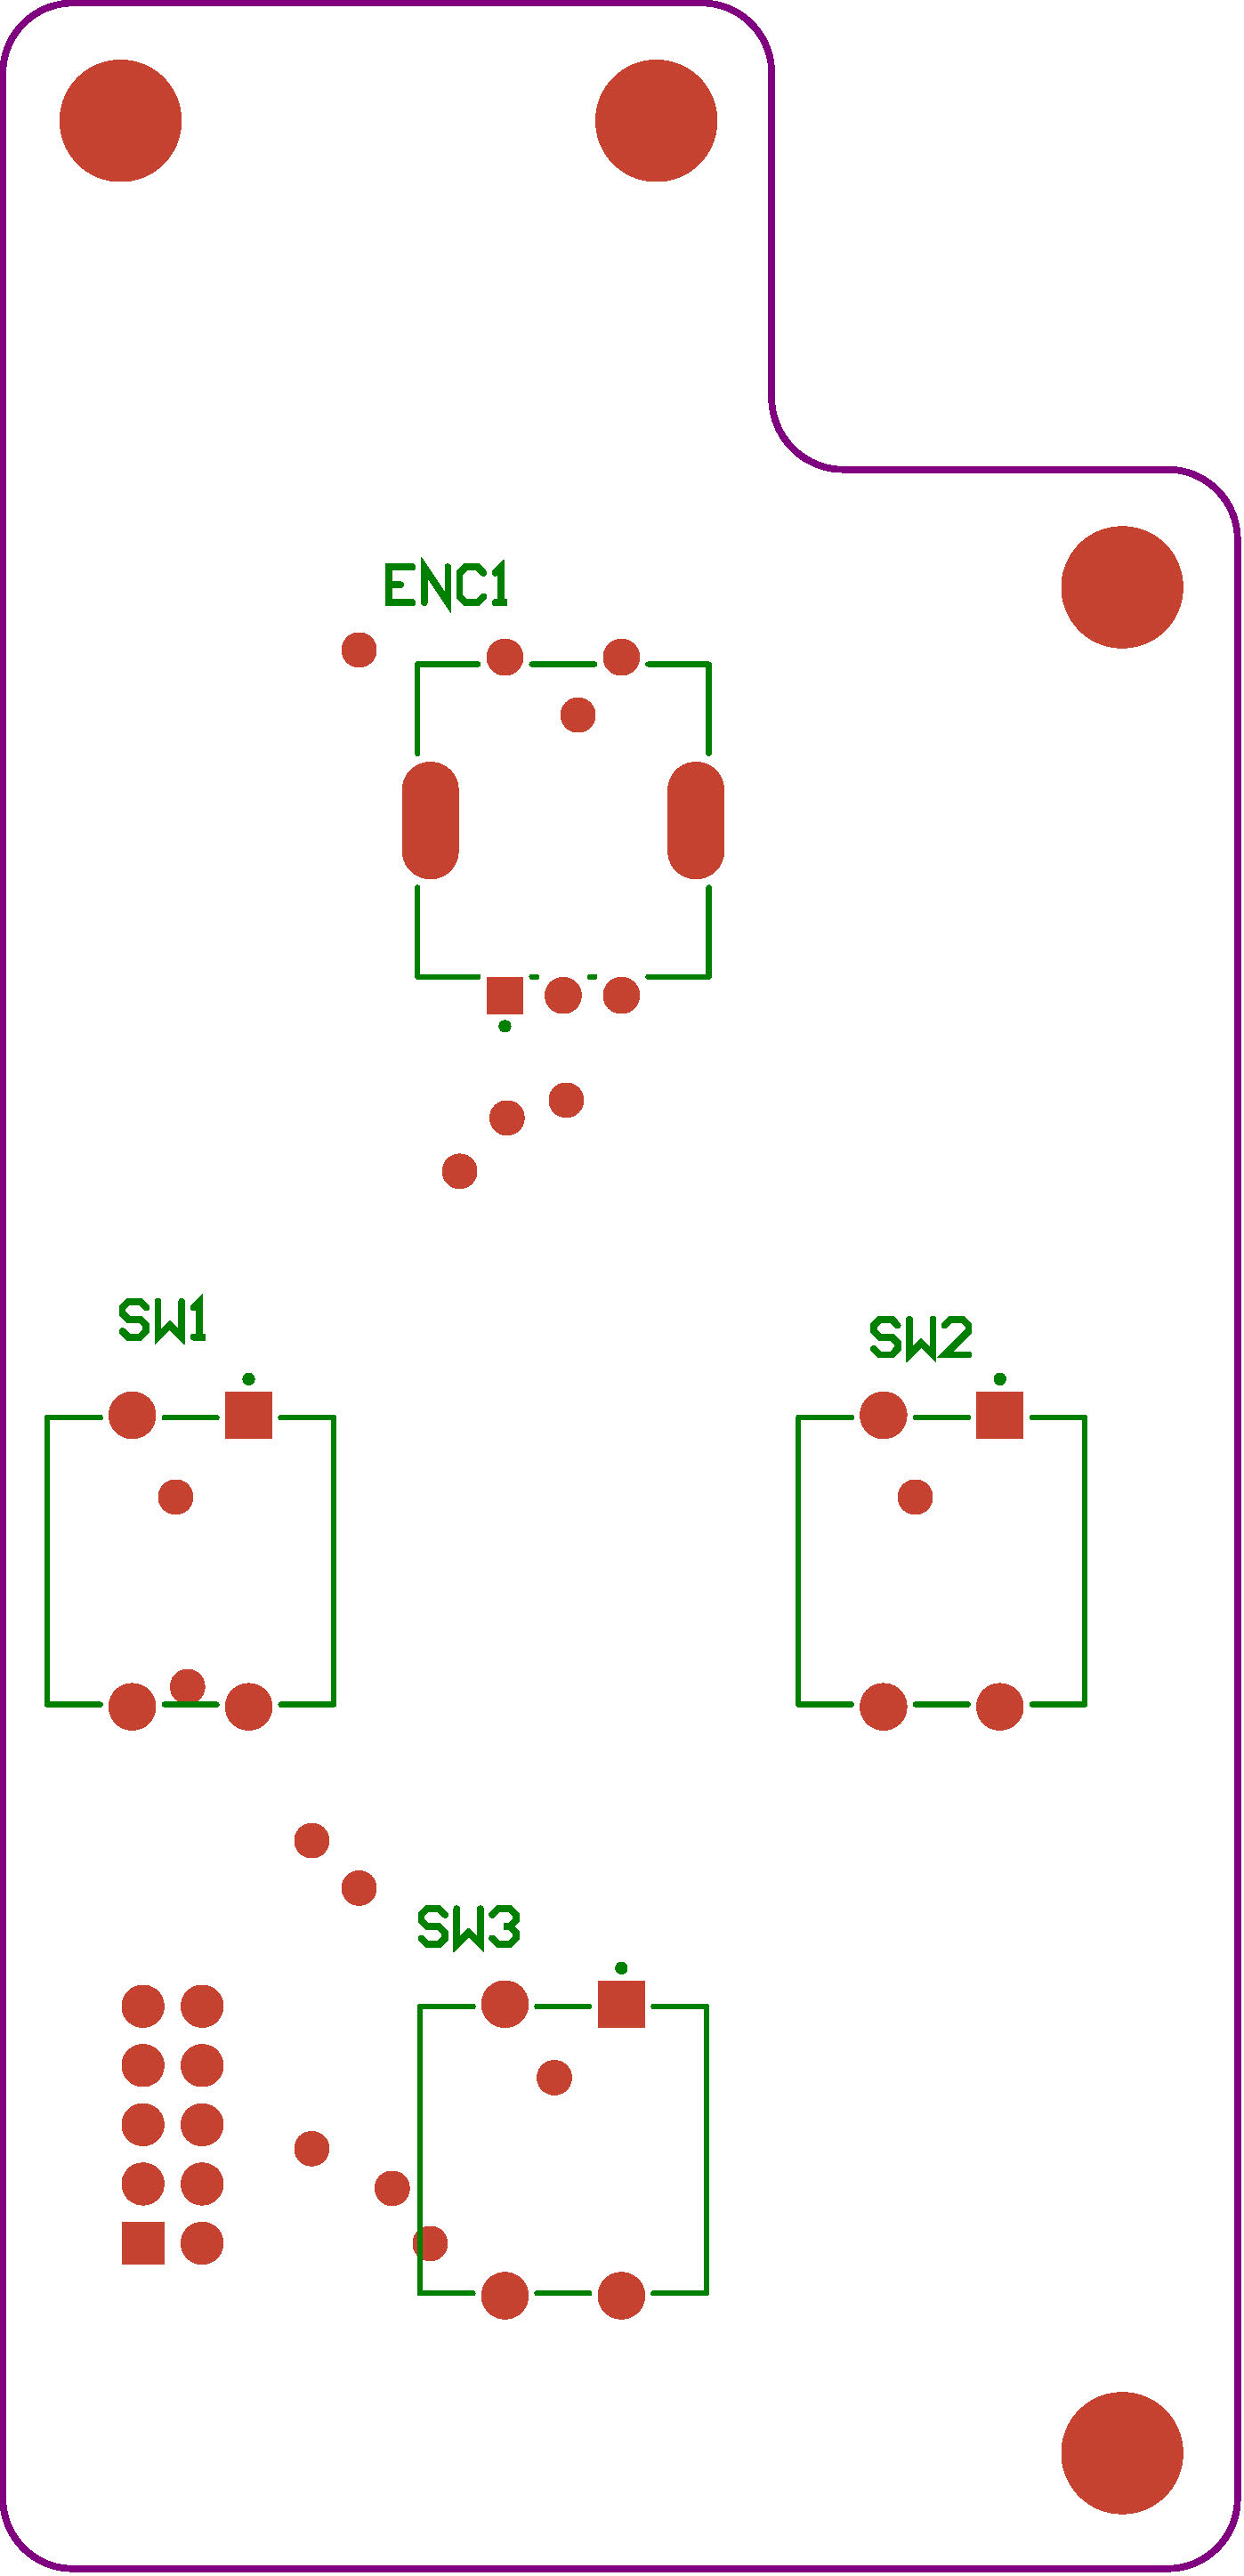
\includegraphics[width=7.5cm]{zalaczniki/przyciski/Przyciski_lewe_Strona_4.jpg} }}%
    \caption{Warstwy opisowe PCB.}
\end{figure}

\begin{sidewaysfigure}
    \begin{center}
        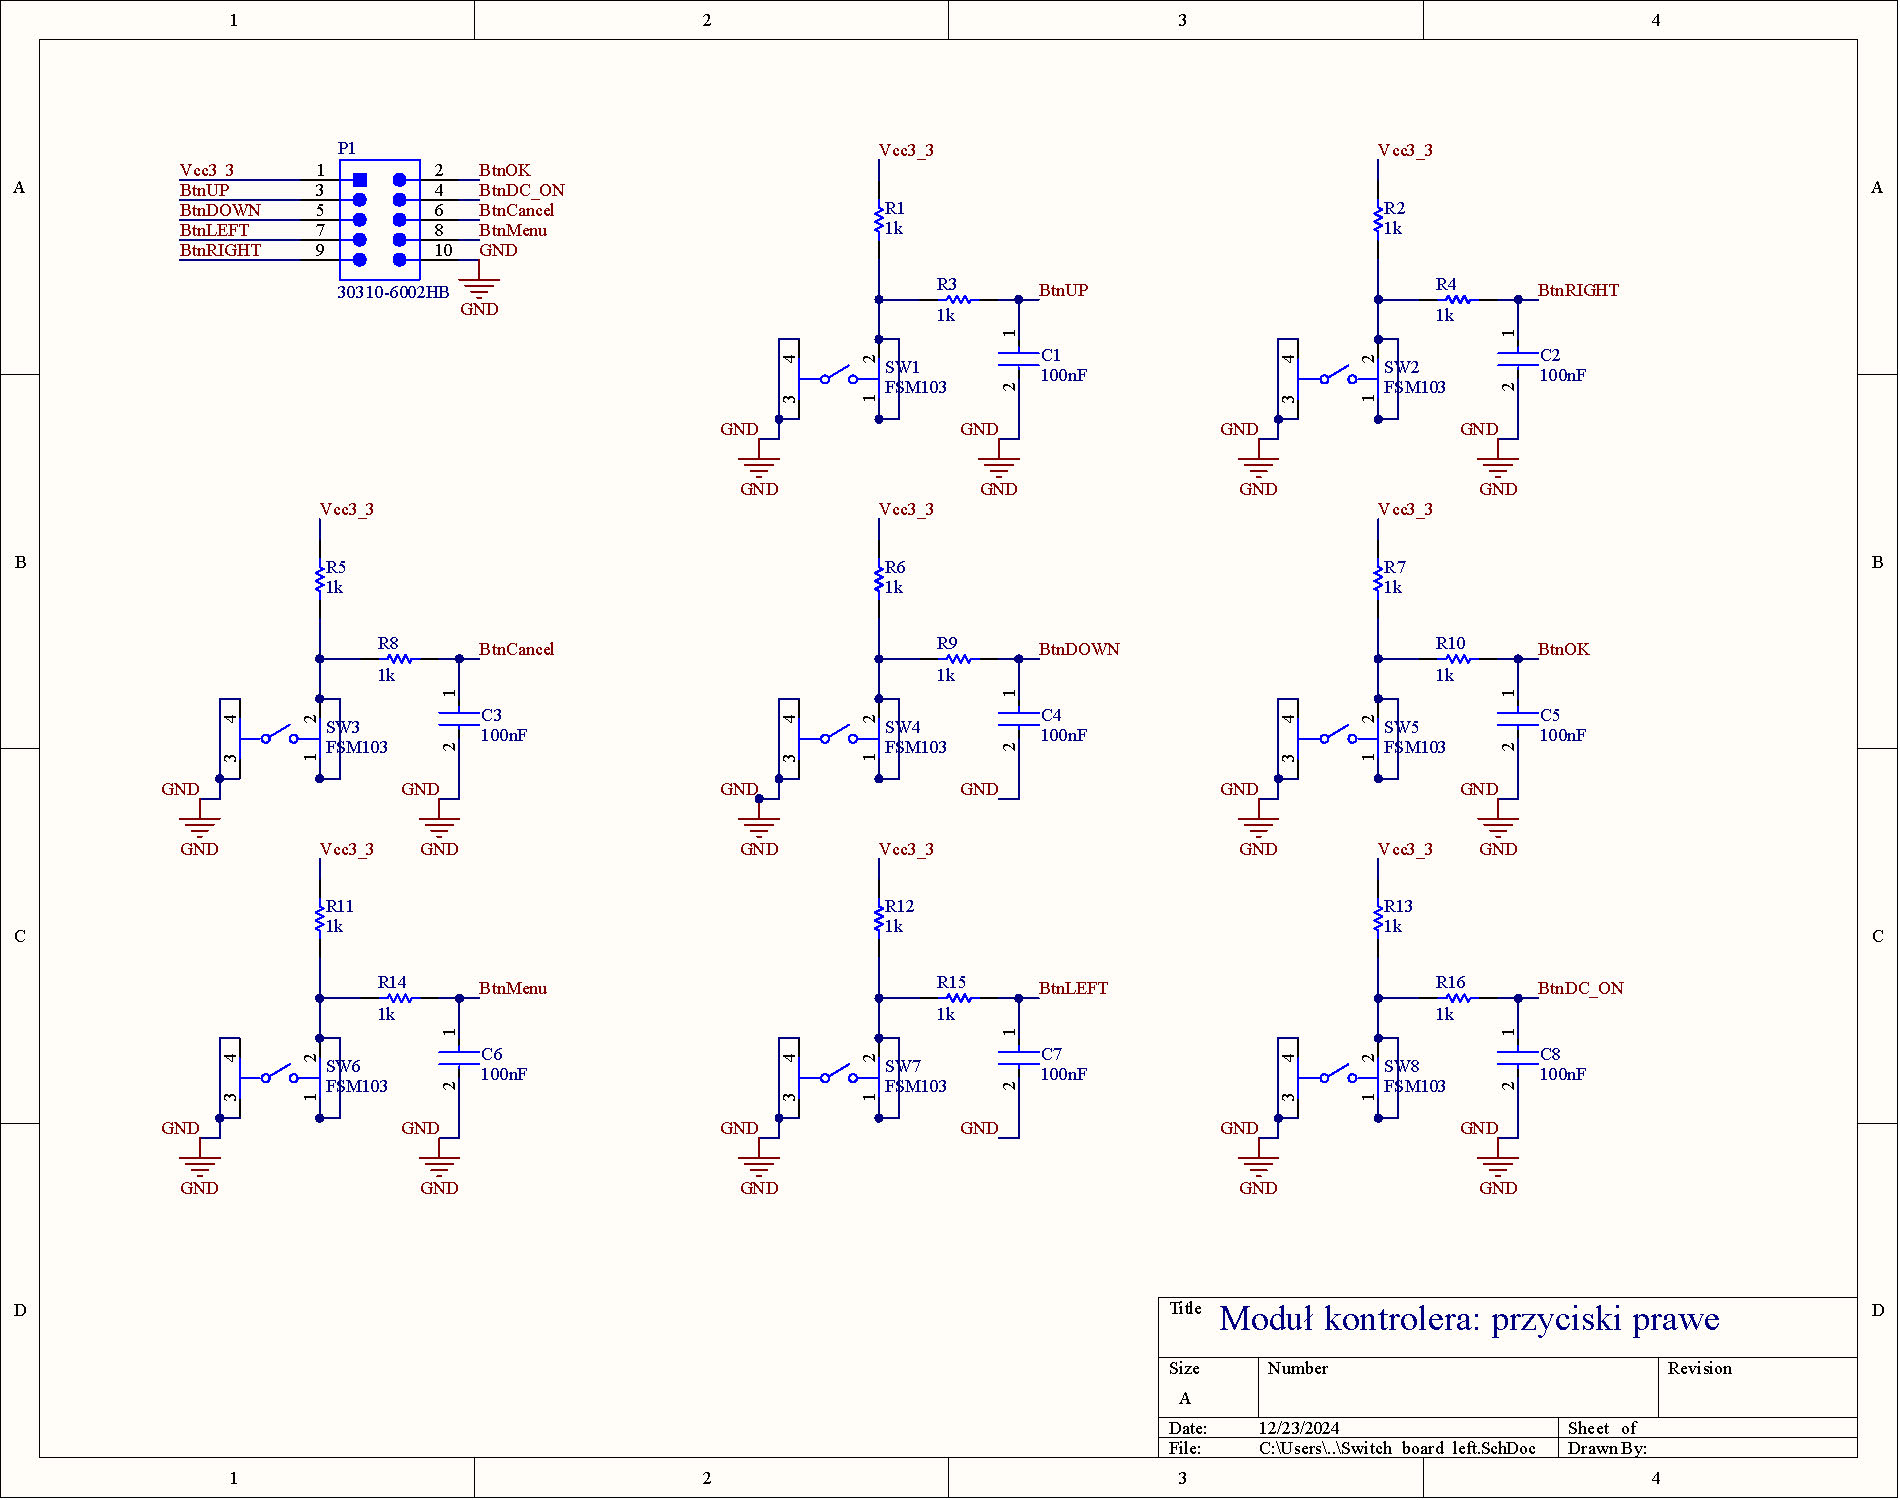
\includegraphics[width = 21cm]{zalaczniki/przyciski/Przyciski_prawe_Strona_1.jpg}
        \caption{Schemat panelu lewego.}
    \end{center}
\end{sidewaysfigure}

\begin{sidewaysfigure}
    \begin{center}
        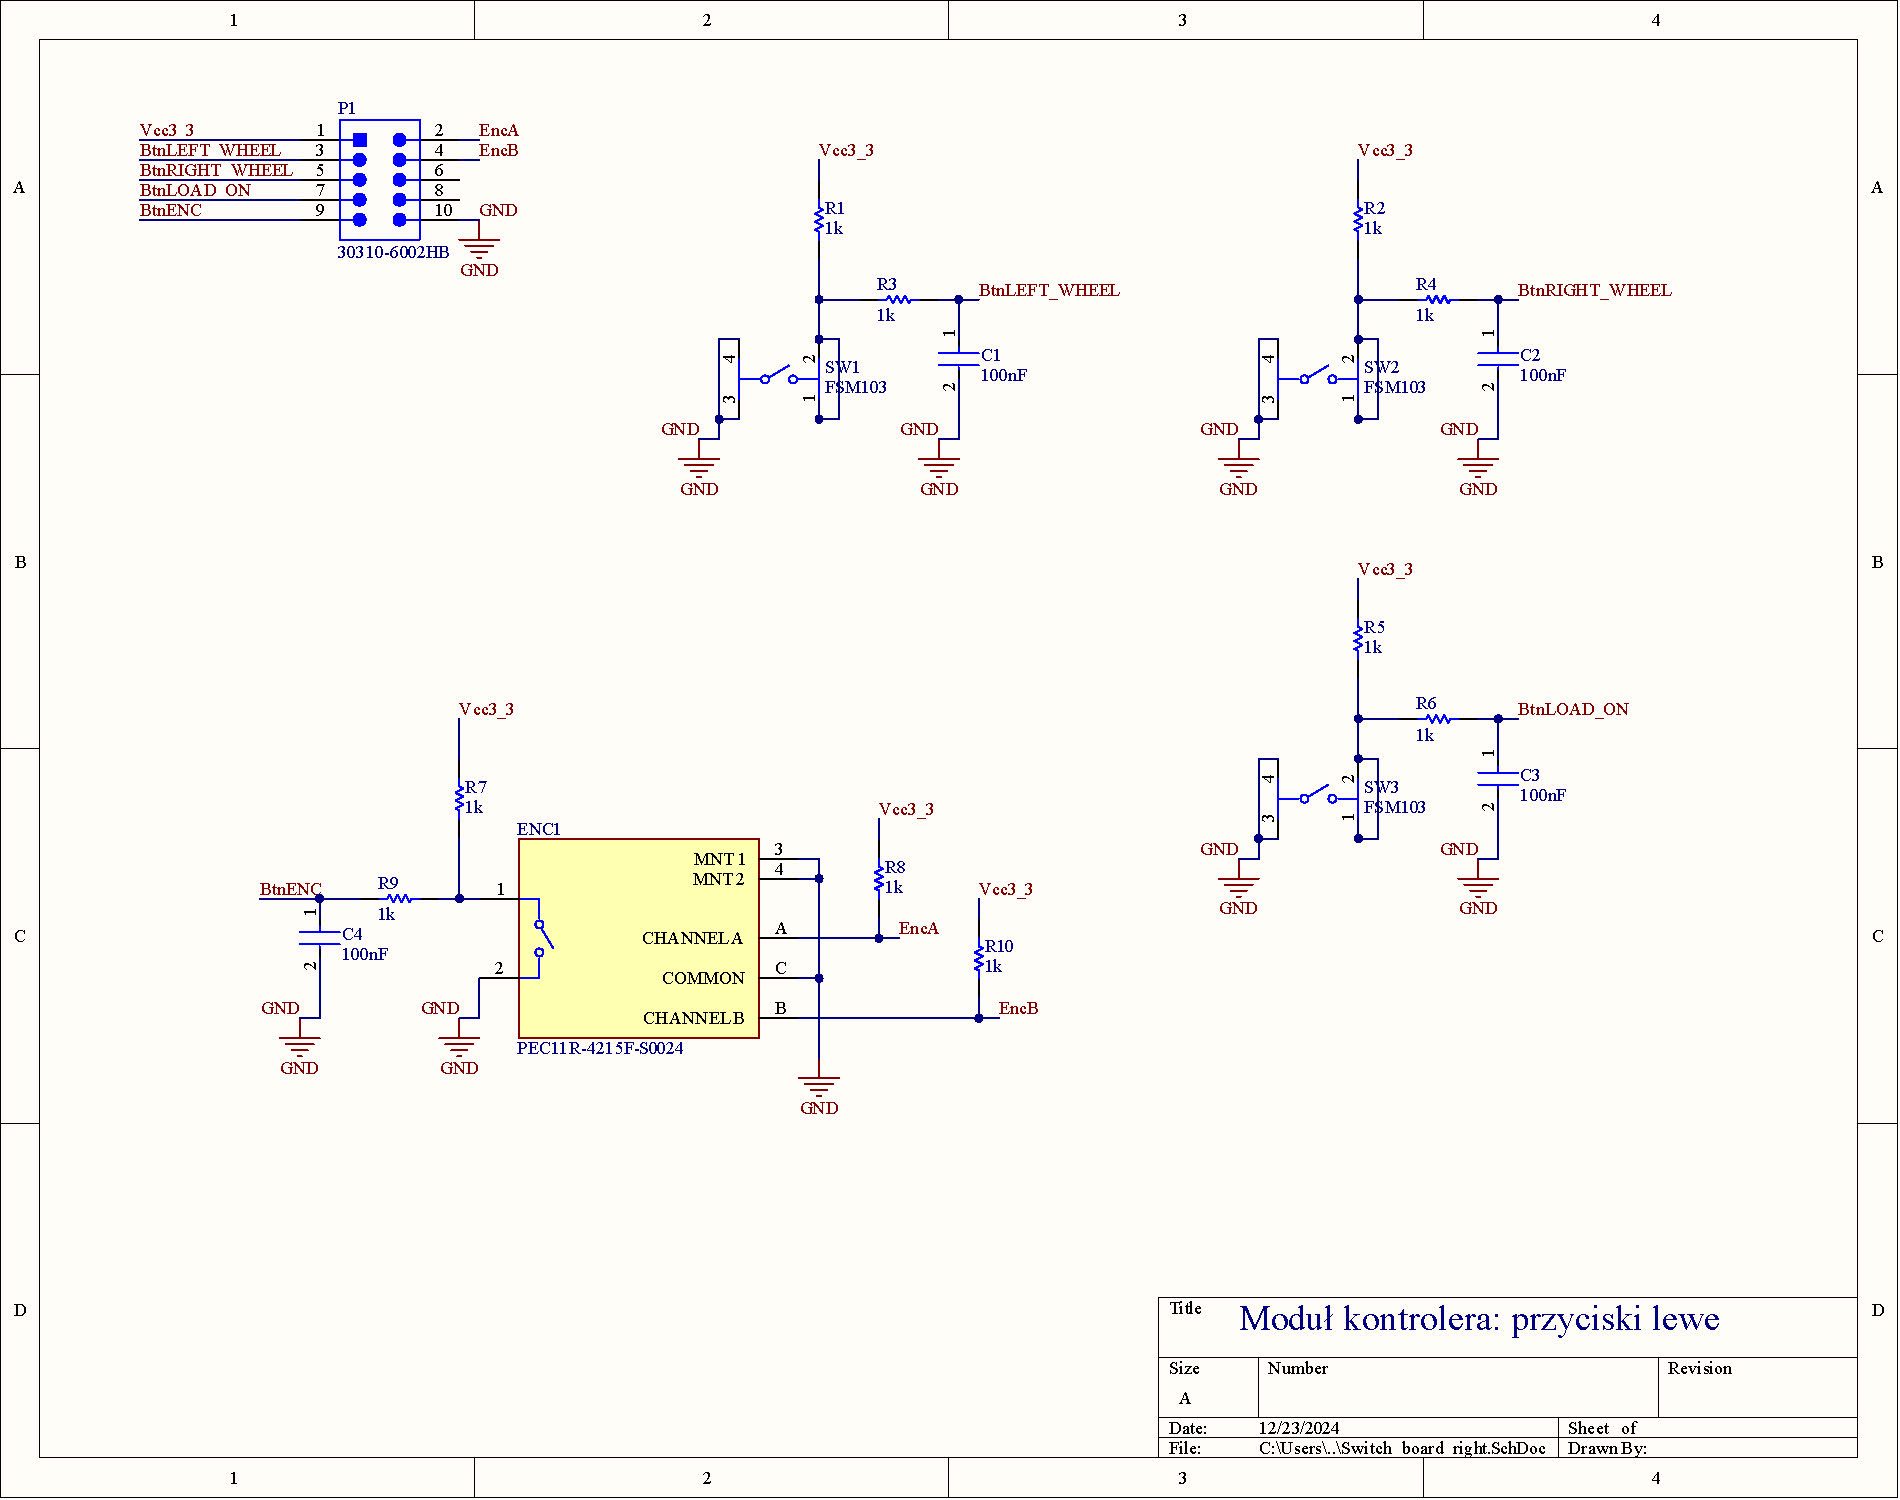
\includegraphics[width = 21cm]{zalaczniki/przyciski/Przyciski_lewe_Strona_1.jpg}
        \caption{Schemat panelu prawego.}
    \end{center}
\end{sidewaysfigure}

\begin{figure}[h!]%
    \centering
 \subfloat[\centering Warstwa górna]{{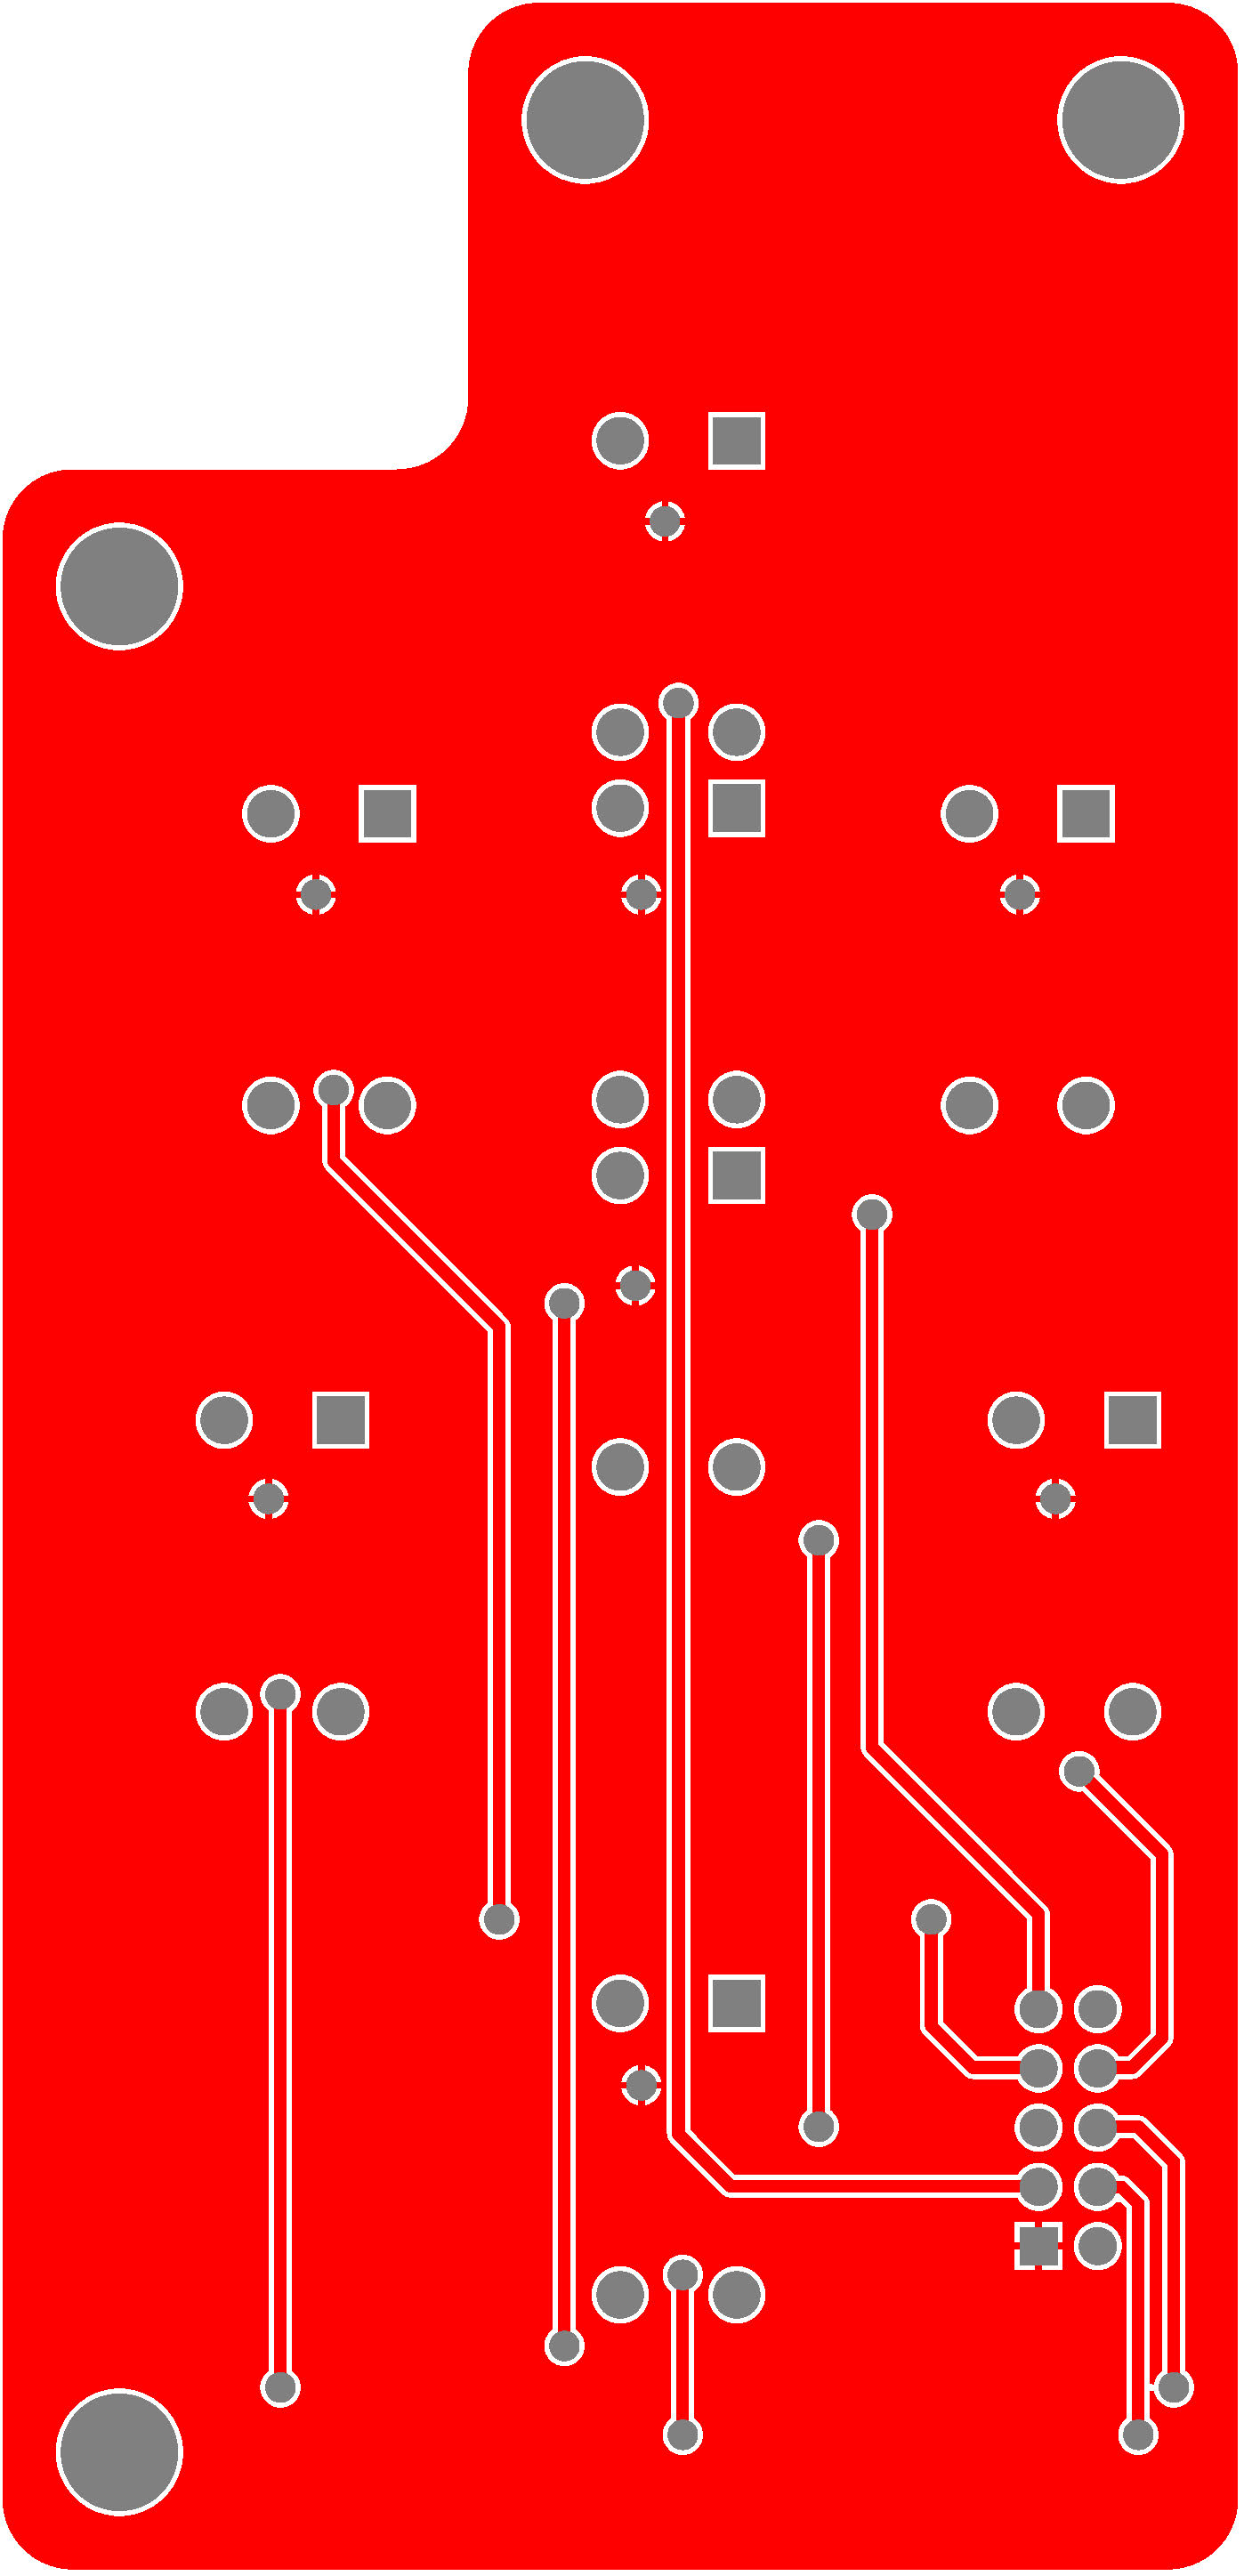
\includegraphics[width=7.5cm]{zalaczniki/przyciski/Przyciski_prawe_Strona_2.jpg} }}%
    \qquad
    \subfloat[\centering Warstwa dolna.]{{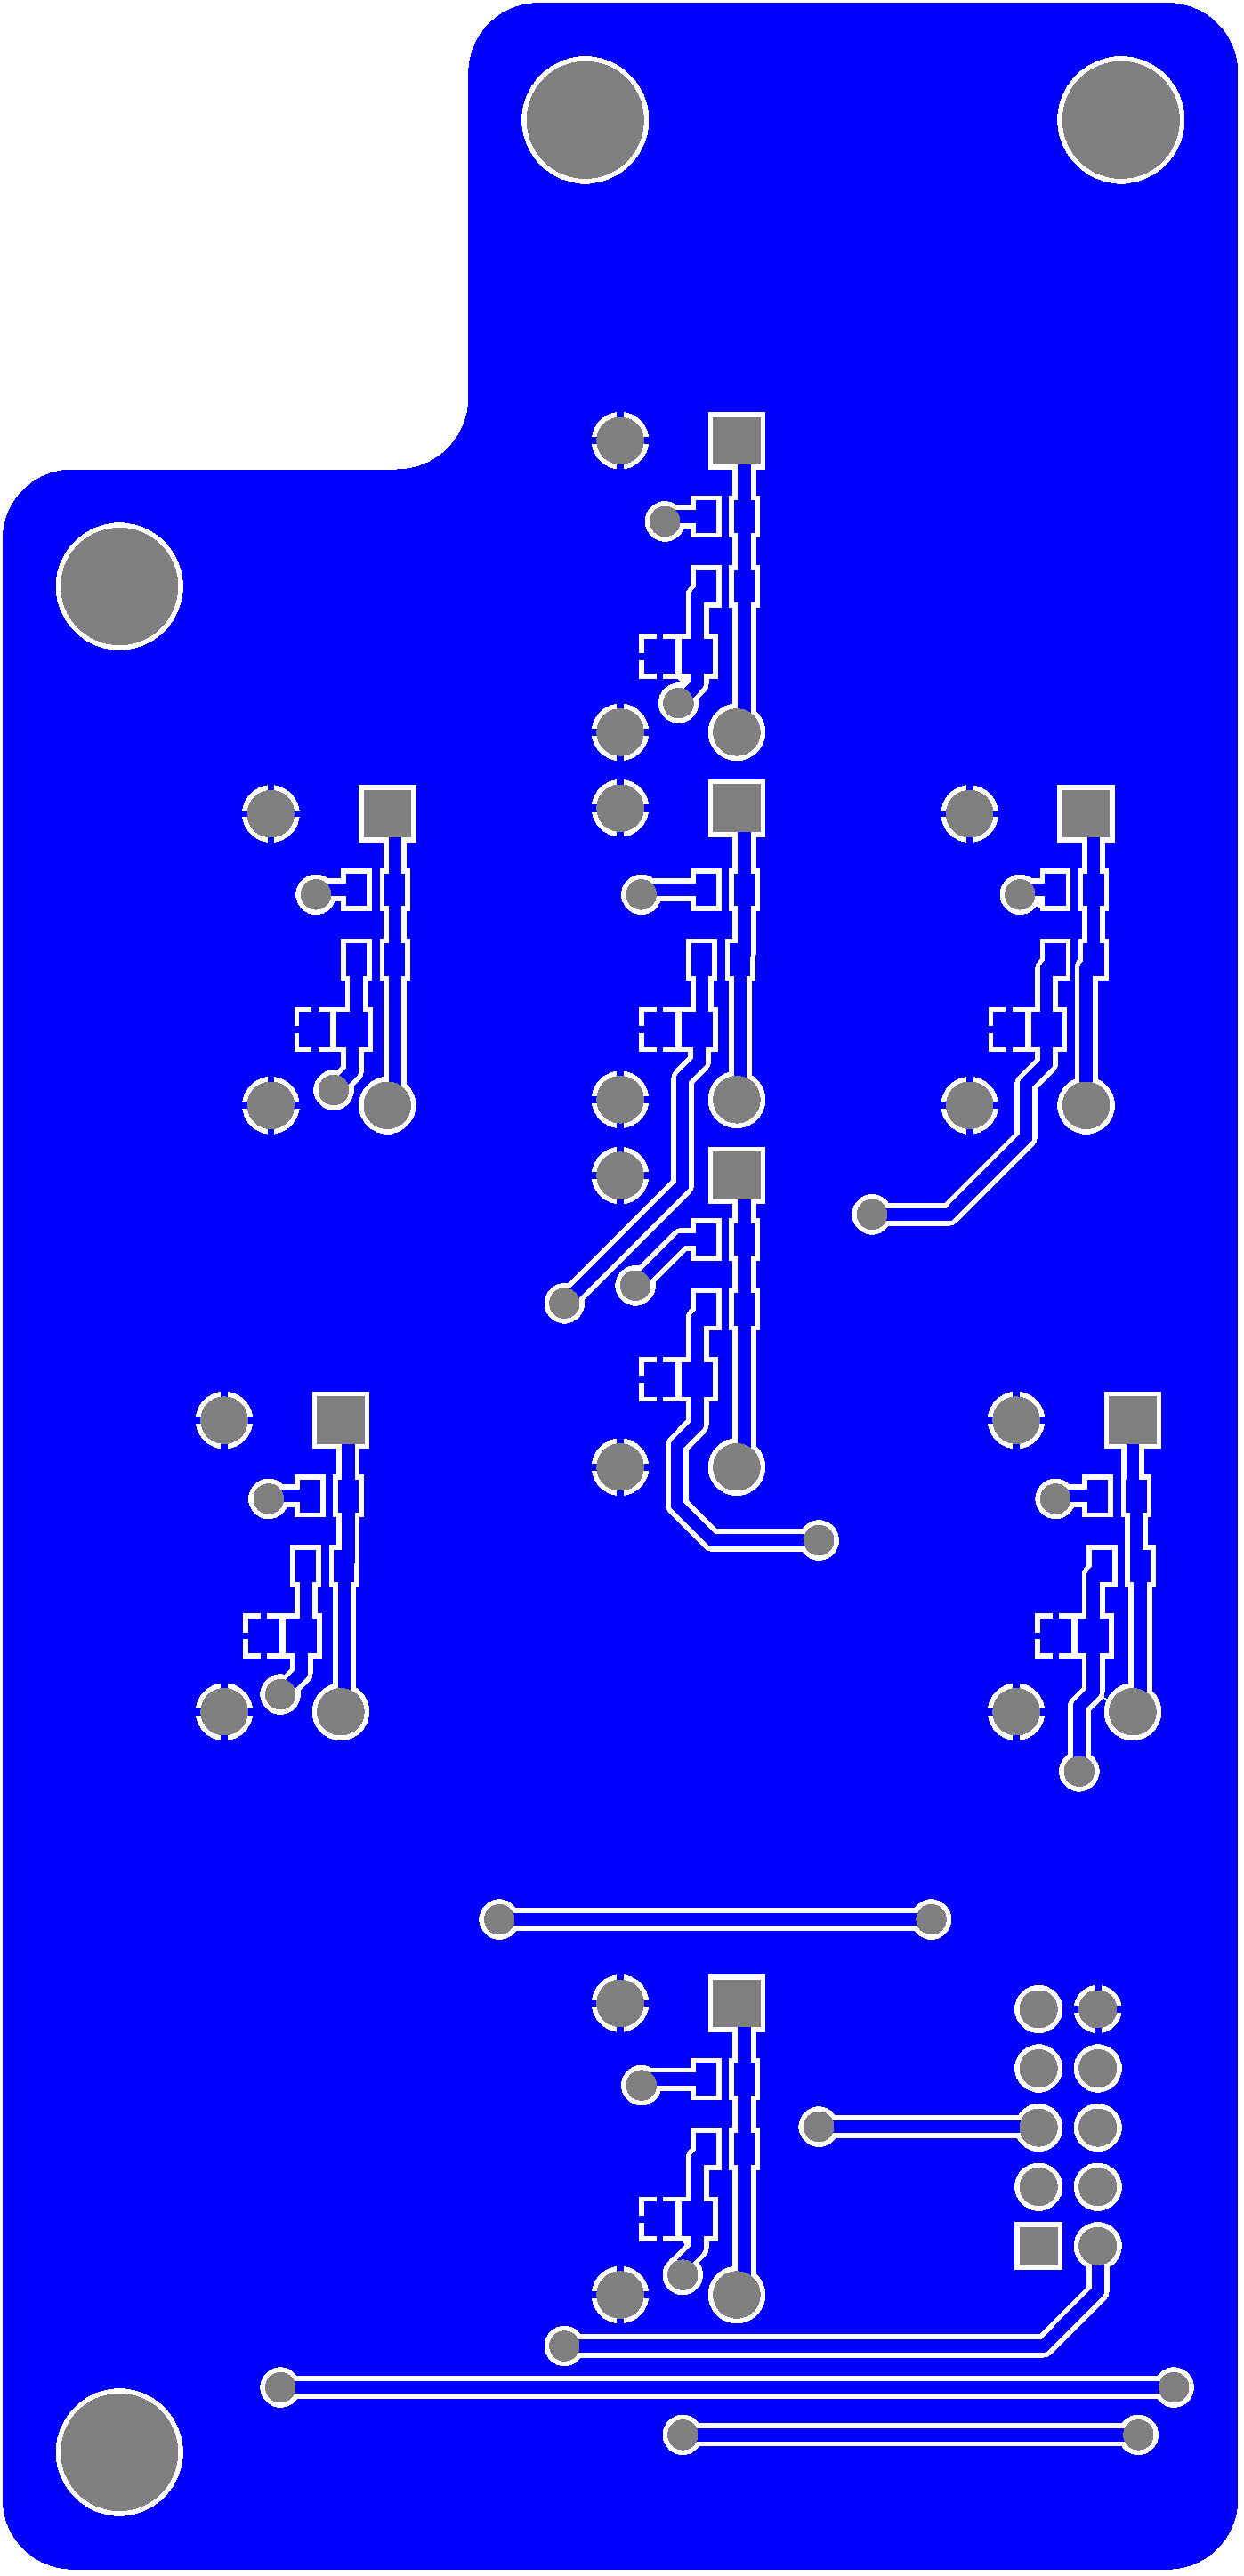
\includegraphics[width=7.5cm]{zalaczniki/przyciski/Przyciski_prawe_Strona_3.jpg} }}%
    \caption{Panel lewy PCB.}
\end{figure}

\begin{figure}[h!]%
    \centering
    \subfloat[\centering Warstwa górna]{{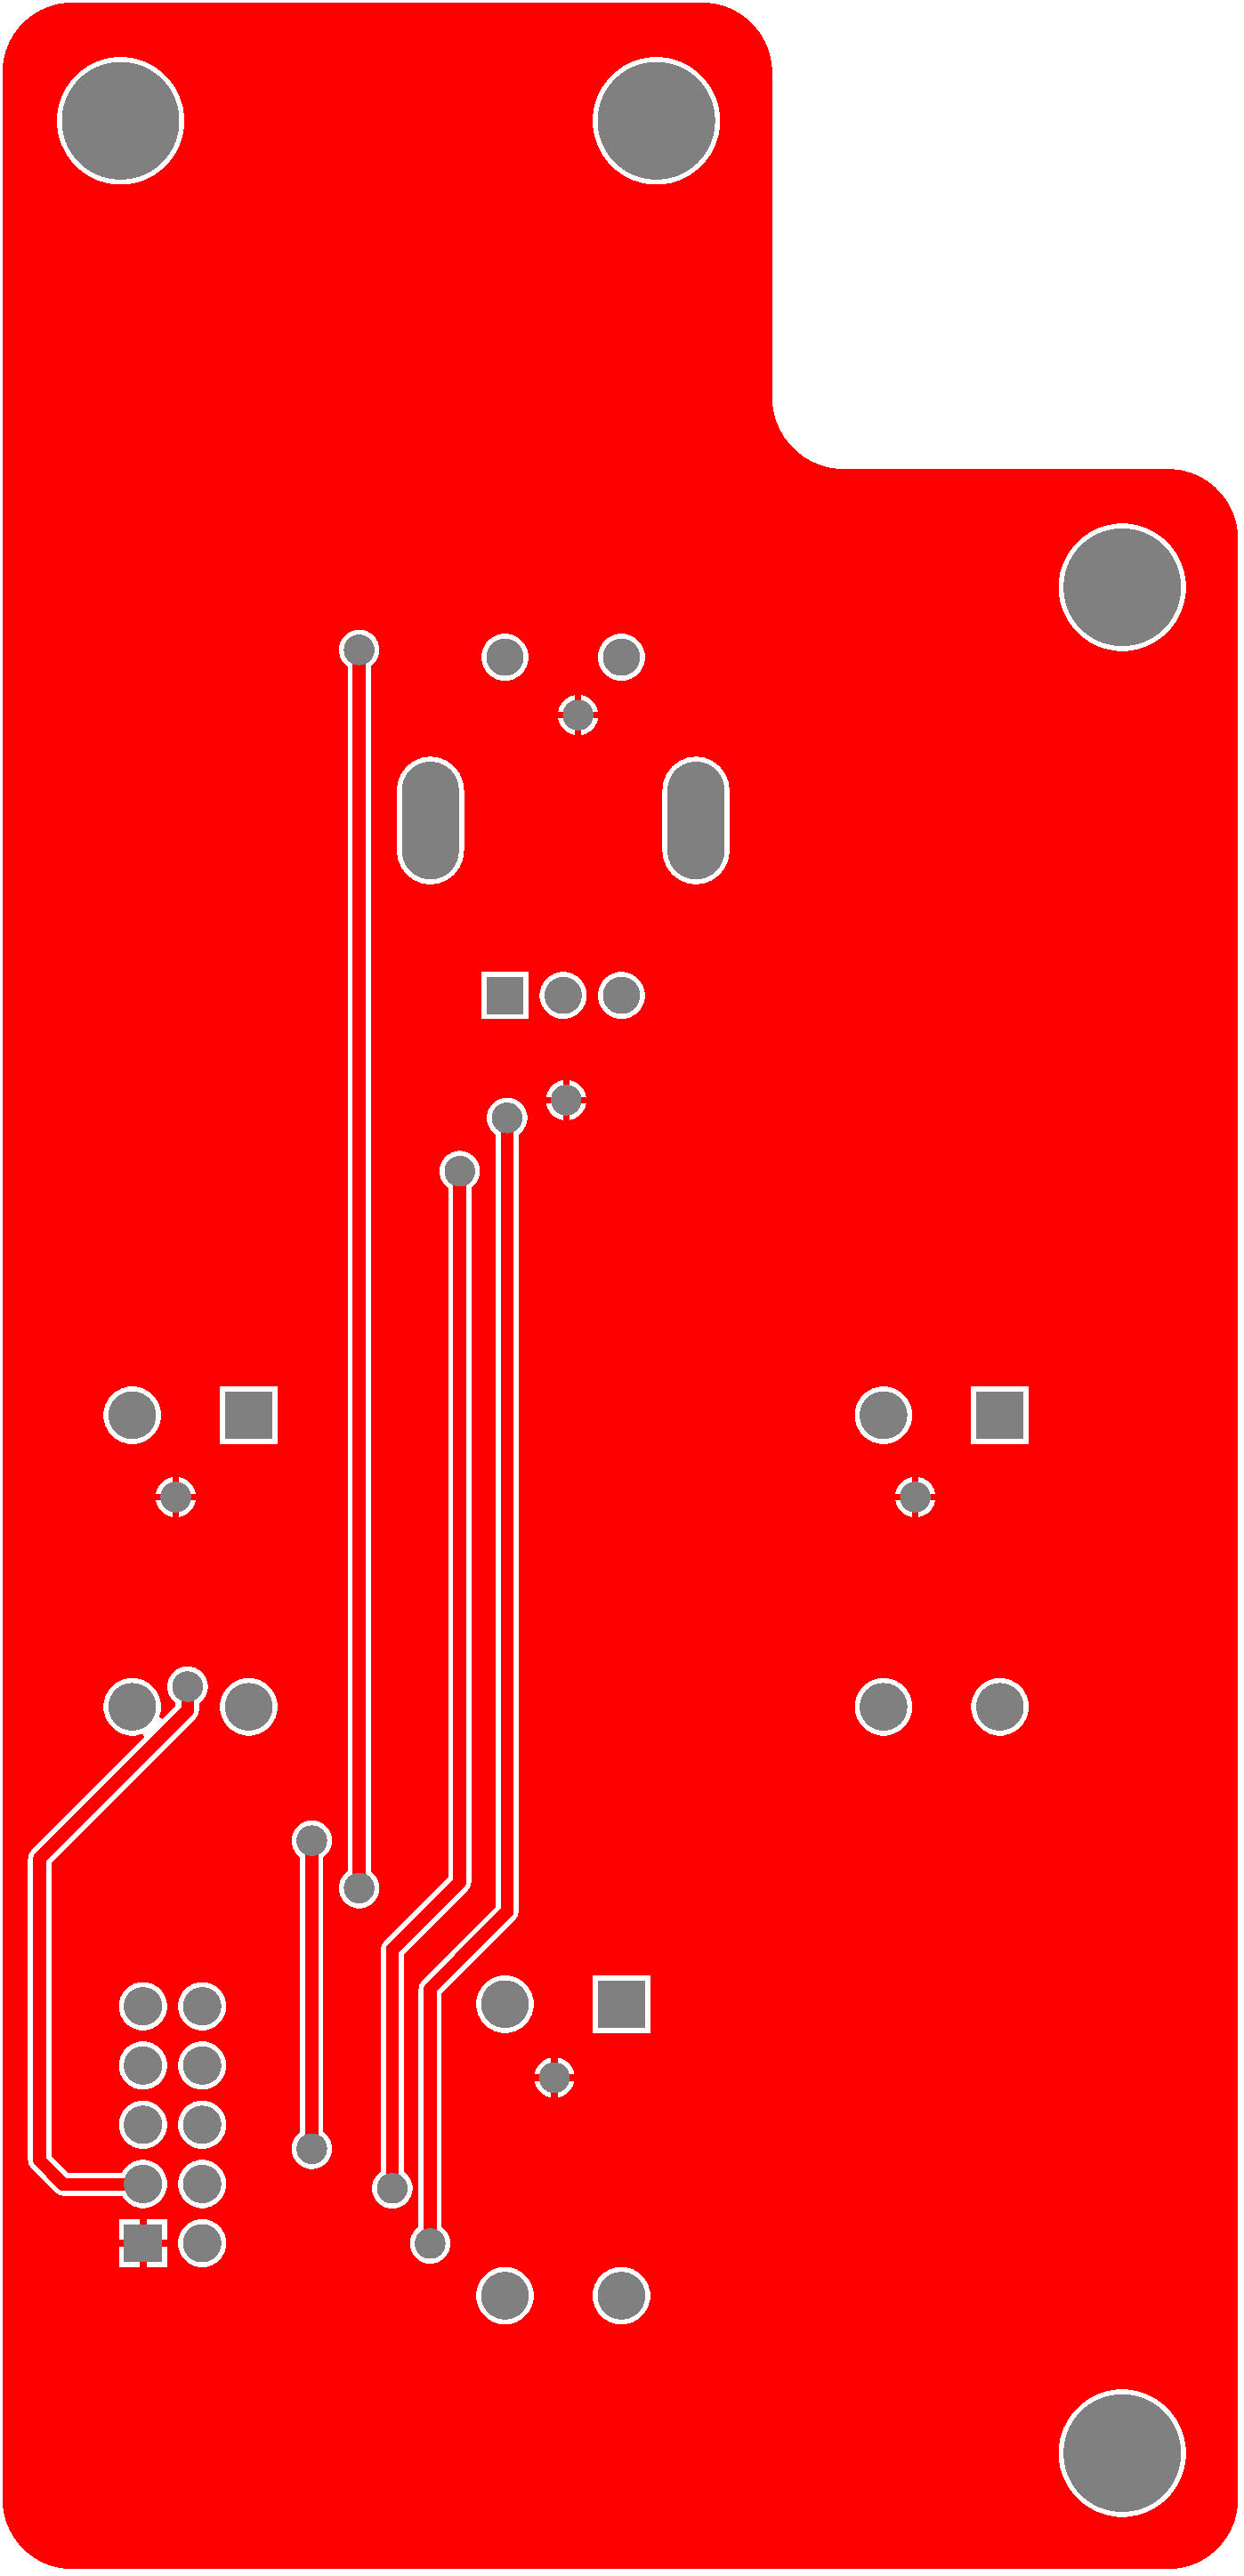
\includegraphics[width=7.5cm]{zalaczniki/przyciski/Przyciski_lewe_Strona_2.jpg} }}%
    \qquad
    \subfloat[\centering Warstwa dolna.]{{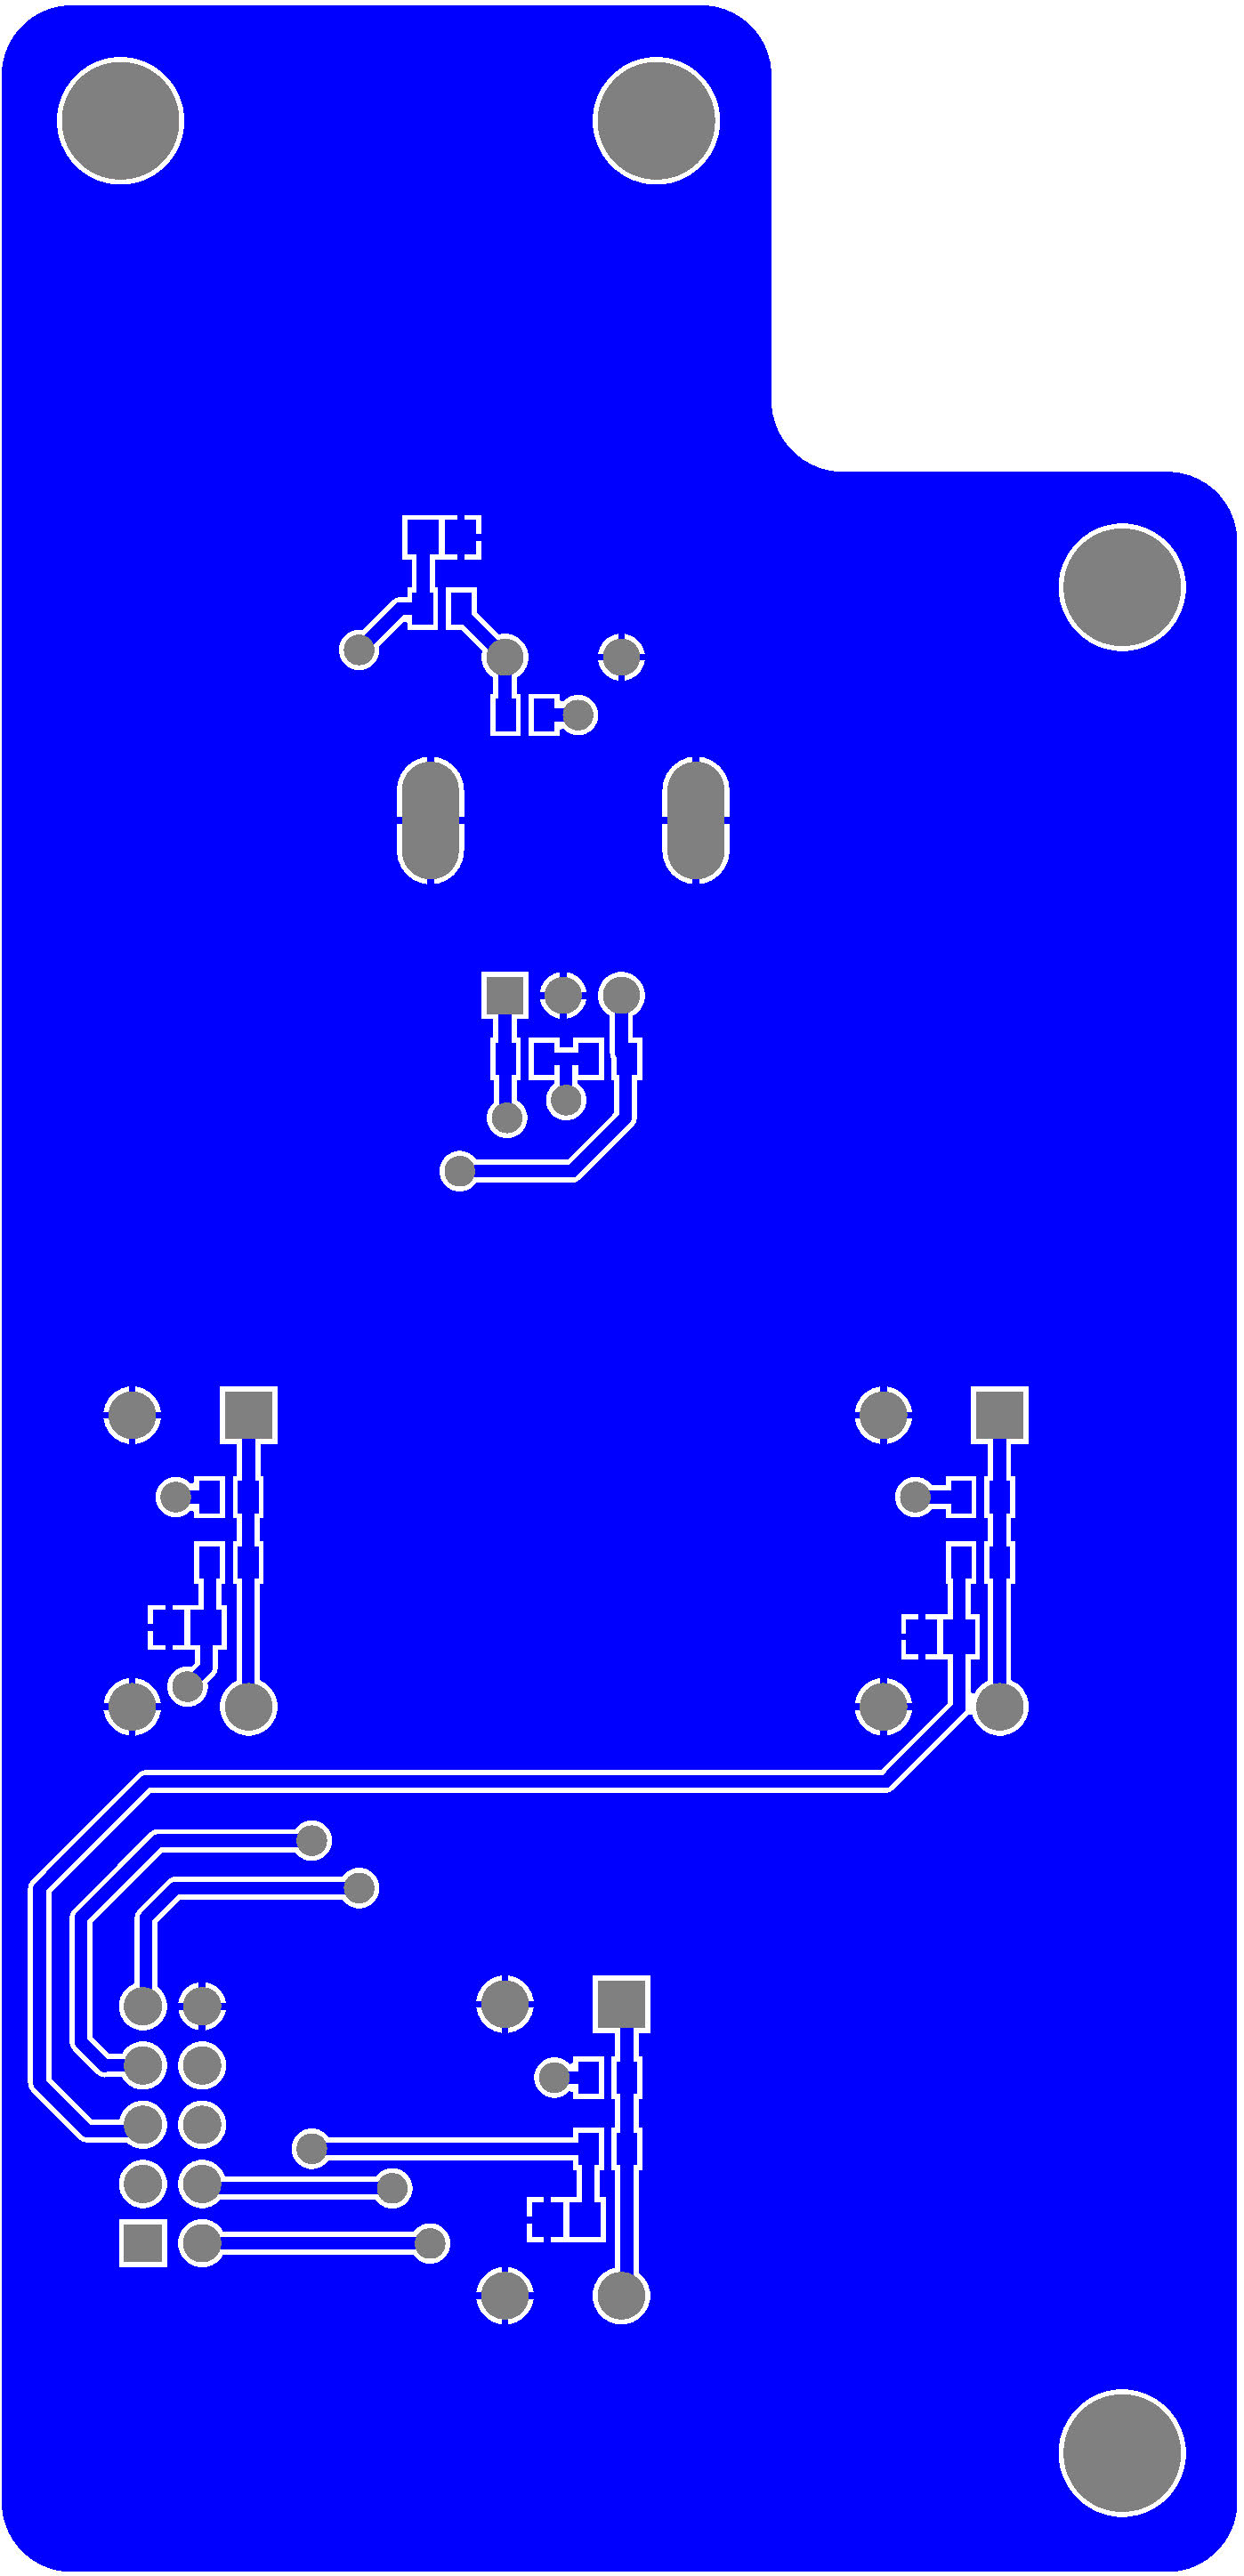
\includegraphics[width=7.5cm]{zalaczniki/przyciski/Przyciski_lewe_Strona_3.jpg} }}%
    \caption{Panel prawy PCB.}
\end{figure}
\endgroup